%% aboensis.tex
%% Copyright 2021 Tommi Syrjönen 
%
% This work may be distributed and/or modified under the conditions of
% the LaTeX Project Public License, either version 1.3 of this license
% or (at your option) any later version. The latest version of this
% license is in http://www.latex-project.org/lppl.txt and version 1.3
% or later is part of all distributions of LaTeX version 2005/12/01 or
% later.
%
% The images of digitized medieval manuscripts that are in this
% document have either been released to use by their creators under
% Creative Commons Attribution 4.0 International (CC BY 4.0) or are
% Public Domain. The licensing details of each image is listed later
% in this file. 
%
% This work has the LPPL maintenance status `maintained'.
% 
% The Current Maintainer of this work is Tommi Syrjänen 
%
% See file MANIFEST-Aboensis.txt to a list of files that make up this
% work.

\documentclass[a4paper]{article}
\usepackage[T1]{fontenc}
\usepackage{fontspec}
\usepackage{xunicode}
\usepackage{xltxtra}
\usepackage{graphicx}
\usepackage{lscape}
\usepackage{longtable}
\usepackage{subfigure}
\usepackage{leading}
\usepackage{xcolor}


\newcommand{\package}[1]{\texttt{#1}}
\newcommand{\feature}[1]{\texttt{#1}}

\newcommand{\samplefont}{\fontsize{16}{16}\abcursivefamily\spaceskip0.2em}
\newcommand{\sample}[1]{{\samplefont #1 \strut}}
\newcommand{\largesample}[1]{\scalebox{2.0}{{\samplefont #1 \strut}}}

\newcommand{\samplebox}[1]{\fbox{\hbox{\sample{#1}}}}

\newcommand{\lettersample}[1]{{\fontsize{18}{18}\fontspec[RawFeature=-calt;]{Aboensis}#1}}
\newcommand{\lombardsample}[1]{{\fontsize{32}{32}\fontspec{Aboensis}\abred{+#1+}}}

\newcommand{\abgreen}[1]{{\addfontfeature{Color=62876E}#1}}
\newcommand{\lombardsampletwo}[1]{{\fontsize{32}{32}\fontspec{Aboensis}\abred{+#1+}\abgreen{+#1/+}}}
\newcommand{\lombardsampleother}[1]{{\fontsize{32}{32}\fontspec{Aboensis}\abred{+#1:+}\abgreen{+#1/+}}}



\newcommand{\cursiveinitialsample}[1]{{\fontsize{64}{64}\fontspec{Aboensis}{+#1+}}}

\newcommand{\topalign}[2]{\hbox{\vbox to \ht#1
    {\hbox{#2}\vfill}}}
\newcommand{\midalign}[2]{\hbox{\vbox to \ht#1
    {\vfill\hbox{#2}\vfill}}}


\newcommand{\ltxenv}[1]{\texttt{#1}}
\newcommand{\ltxncmd}[1]{\texttt{\textbackslash{}#1}}
\newcommand{\ltxcmd}[2]{\texttt{\textbackslash{}#1\{#2\}}}
\newcommand{\ltxcmdtwo}[3]{\texttt{\textbackslash{}#1\{#2\}\{#3\}}}
\newcommand{\ltxcmdthree}[4]{\texttt{\textbackslash{}#1\{#2\}\{#3\}\{#4\}}}
\newcommand{\ltxcmdfour}[5]{\texttt{\textbackslash{}#1\{#2\}\{#3\}\{#4\}\{#5\}}}



\newbox\showletterbox
\newlength\showletterboxheight
\newlength\showletterboxwidth
\newcommand{\showlettertitle}[2]{%
  \setbox\showletterbox\hbox{\lettersample{#1}}%
  \showletterboxheight=2.5em%
  \showletterboxwidth=2em%
  \hbox{\raise1em\hbox{\fbox{\hbox to \showletterboxwidth{\vbox to\showletterboxheight{%
        \hbox to \showletterboxwidth{\tiny\hfill#2\hfill}\vspace{1mm}\vfill%
        \hbox to \showletterboxwidth{\hfill\hbox{\hfill\lettersample{#1}\hfill}\hfill}\vspace{2mm}}}}}}}

\newcommand{\showlettertitletwo}[2]{%
  \multicolumn{2}{l@{ }}{\setbox\showletterbox\hbox{\lettersample{#1}}%
  \showletterboxheight=2.5em%
  \showletterboxwidth=5em%
\hbox{\raise1em\hbox{\fbox{\hbox to \showletterboxwidth{\vbox to\showletterboxheight{%
        \hbox to \showletterboxwidth{\tiny\hfill#2\hfill}\vspace{1mm}\vfill%
        \hbox to \showletterboxwidth{\hfill\hbox{\hfill\lettersample{#1}\hfill}\hfill}\vspace{2mm}}}}}}}}

\newcommand{\abred}[1]{{\addfontfeature{Color=B1523E}#1}}
\newcommand{\abdarkred}[1]{{\addfontfeature{Color=4D231C}#1}}

\usepackage{aboensis}
\abtildes
\setcounter{tocdepth}{2}


\begin{document}


\bibliographystyle{plain}

\title{\fontsize{36}{36}\fontspec[BoldFont=Aboensis]{Aboensis}\abcapital{A}boensis}
\author{Tommi Syrjänen}

\maketitle


\begin{center}
  
\begin{minipage}{10.5cm}
  {{\fontsize{16}{19}\abcursivefamily
      \abstartchapter{Q}{\abcapital{U}o usque tandem abutere,
        \abcapital{C}atilina, pati-}{entia nostra? \abcapital{Q}u~a diu
        etiam furor jste}
      \abl{tuus nos eludet? \abcapital{Q}uem ad finem sese effrena-}
      \abl{ta jactabit audacia? \abcapital{N}ihilne te nocturn~u prae}
      \abl{sidium palati, nihil urbis vigiliae, nihil timor }
      \abl{populi, nihil concursus bono[rum] omnium, nihil hic }
      \abl{munitissim[us] habendi senat[us] locus, nihil horum }
      \abl{ora voltus[que] moverunt? \abcapital{P}atere tua consilia non }
      \abl{sen[tis], constrict~a iam ho[rum] omnium scientia te-}
      \abl{neri coniurationem tuam non vides? \abcapital{Q}uid pro}
      \abl{xima, quid su[per]iore nocte ege[ris], ubi fue[ris], quos }
      \abl{convocave[ris], quid consilii ceperis, quem nostr~u }
      \abl{ignorare arbitraris? \mbox{} \mbox{} \abotherrubric{!*************>>>>><}}
}}

\end{minipage}
\end{center}

\thispagestyle{empty}



\newpage


\newpage


The text in the previous page is the beginning of Marcus Tullius
Cicero's \emph{Oratio in catilinam primo} that has been used to set
typographical speciments at least since the days of Gianbattista Bodoni
(1740–1813). In modern fonts its text reads:

\thispagestyle{empty}

\begin{quote}
  Quo usque tandem abutere, Catilina, patientia nostra? quam diu etiam
  furor iste tuus nos eludet? quem ad finem sese effrenata iactabit
  audacia? Nihilne te nocturnum praesidium Palati, nihil urbis
  vigiliae, nihil timor populi, nihil concursus bonorum omnium, nihil
  hic munitissimus habendi senatus locus, nihil horum ora voltusque
  moverunt? Patere tua consilia non sentis, constrictam iam horum
  omnium scientia teneri coniurationem tuam non vides? Quid proxima,
  quid superiore nocte egeris, ubi fueris, quos convocaveris, quid
  consilii ceperis, quem nostrum ignorare arbitraris? 
\end{quote}

C.\,D. Yonge \cite{yonge} translated the paragraph as:

 \begin{quote}
   When, O Catiline, do you mean to cease abusing our patience? How
   long is that madness of yours still to mock us? When is there to be
   an end of that unbridled audacity of yours, swaggering about as it
   does now? Do not the nightly guards placed on the Palatine Hill—do
   not the watches posted throughout the city—does not the alarm of the
   people, and the union of all good men—does not the precaution taken
   of assembling the senate in this most defensible place—do not the
   looks and countenances of this venerable body here present, have any
   effect upon you? Do you not feel that your plans are detected? Do
   you not see that your conspiracy is already arrested and rendered
   powerless by the knowledge which every one here possesses of it?
   What is there that you did last night, what the night before—where
   is it that you were—who was there that you summoned to meet
   you—what design was there which was adopted by you, with which you
   think that any one of us is unacquainted?
 \end{quote}


\vfill


The font Aboensis is copyrighted by Tommi Syrjänen, 2021. It may be
used and distributed under the Open Font License 1.1 (see
page \pageref{pg_license} for details).

The documentation and LaTeX style files are also copyrighted by Tommi
Syrjänen, 2021, and they may be distributed under the terms of Latex
Project Public License 1.3c (see the accompanying file
\texttt{lppl.txt} for details or refer to
\texttt{http://www.latex-project.org/lppl.txt}).

The image files showing original medieval documents are either Public
Domain or are licensed under Creative Commons Attribution 4.0
International License by the organizations that digitized them. Their
individual licenses are listed on pages
\pageref{image_license_start}–\pageref{image_license_end}.


\newpage

\nocite{aboensis_77}
\nocite{rea1996}
\nocite{df}
\nocite{sdhk}
\nocite{cf}
\nocite{coda}
\nocite{codc}
\nocite{suvanto1995}
\nocite{keranen2018}
\nocite{seppala09}
\nocite{vilkuna98}
\nocite{derolez03}
\nocite{valtionarkisto77}
\nocite{makela_alitalo07}
\nocite{jansson98}
\nocite{oxenstierna04}
\nocite{wiktorsson04}
\nocite{svensson74}
\nocite{jansson36}
\nocite{thulin36}
\nocite{voionmaa36}
\nocite{melander1892}
\nocite{voudintilit}
\nocite{dokumentteja1}

\begin{center}
\fbox{
  \begin{minipage}{0.8\linewidth}
    \begin{center}
      \textbf{The Short Version of Important Stuff}
    \end{center}
    \begin{itemize}
    \item \Aboensis{} is a free OpenType/CFF font intended for
      emulating late medieval manuscripts. 

  \item It should be used in relatively large size (14+ points).

  \item It is licensed under Open Font License (see the end of the
    document for details).

  \item It is a 15th century typeface. It contains a large number of
    symbols (see pages
    \pageref{pg:symbols_start}–\pageref{pg:symbols_end}) that are no
    longer in common use but it lacks many symbols that are nowadays
    in common use.

  \item It has a large number of OpenType features that control its
    behavior. See section \ref{sec_opentype} for details.
    The "Standard ligatures" (\textrm{liga}) and "Contextual
    alternates" (\textrm{calt}) features should be always turned on
    for proper function of the font. 

  \item It is designed to be used with XeLaTeX. See section
    \ref{sec_latex_style} for details.
 
  \item \Aboensis{} works in recentish programs. Some old font
    renderers will mess up the spacing between letters. This happens
    at least in some old versions of MS Word. Newer programs shouldn't
    have problems. However, some care is necessary when using
    highlighted initials symbols with XeLaTeX, see
    section \ref{ssec_correct_forms} for details. 

\end{itemize}
  \end{minipage}
}
\end{center}

\begin{table}
  \centering
  \fbox{\begin{minipage}{0.9\linewidth}
    
    \begin{itemize}
    \item Abbreviate with brackets:
      \begin{center}
        \begin{tabular}{cccc}
          \sample{eorum} & $\Longrightarrow$ & \sample{eo[rum]} \\
          eorum & & eo[rum] 
        \end{tabular}
      \end{center}
      
    \item Add an abbreviation symbol over a letter by preceding it
      with tilde or single quote (use \ltxncmd{abtildes} to make tilde
      regular letter):
      \begin{center}
        \begin{tabular}{cccc}
          \sample{ecc~ia} & \sample{'tminus} \\
          ecc~ia & 'tminus 
        \end{tabular}
      \end{center}
  
    \item Place a letter as a superscript using a grave accent:
      \begin{center}
        \begin{tabular}{cccc}
          \sample{iiii`c}  \\
          iiii`c
        \end{tabular}

      \end{center}

    \item Use asterisk to prevent initial and final forms as needed:
      \begin{center}
        \begin{tabular}{cccc}
          \sample{non} & $\Longrightarrow$ & \sample{*non*} \\
          non & & *non*
        \end{tabular}

      \end{center}        
      \item Add red highlighting to capital letters by writing the
        letter three times on top of itself: first with text color,
        then with the highlight preceded by a slash, and
        finally in darker highlight color with two slashes:
        \begin{center}
          \begin{tabular}{ccccc}
            \sample{A} & \sample{\abred{/A}} & \sample{\abdarkred{//A}}
 &
            $ \Longrightarrow$ & \sample{\abcapital{A}} \\
            A & {\color{abred}/A} & {\color{abdarkred}//A}  & & 
          \end{tabular}
        \end{center}
        With XeLaTex you can use command
        \texttt{\textbackslash{}abcapital} to add a highlighted
        capital.

      \item Enter Lombardic initials by surrounding the letter with
        '+' signs.
        \begin{center}
          \begin{tabular}{cccc}
            \sample{\abred{A}} & $\Rightarrow$ &
            \sample{\abred{+A+}} \\
            {\color{red} A} & &    {\color{red}+A+} \\
          \end{tabular}
        \end{center}
      \item Enter cursive initials by surrounding the letter with two
        '+' signs and use font size 5.5 times larger than the main
        body
        \begin{center}
          \begin{tabular}{cccc}
            \sample{A} & $\Rightarrow$ &
            \scalebox{2.0}{\sample{++A++}} \\
            {A} & &    {++A++} \\
          \end{tabular}
        \end{center}
      \item Prevent uneven line spacing in XeLaTex with \ltxcmd{abl}{line}.
    \end{itemize}
  \end{minipage}}
  \caption{A quick partial guide to special symbols}
  \label{tab_special}
\end{table}


\newpage 

\tableofcontents


\mbox{}
\newpage


\section{Introduction}

\begin{table}
  \centering
  \begin{tabular}{lllllllllll}
    \lettersample{A} & 
    \lettersample{B} & 
    \lettersample{C} & 
    \lettersample{D} & 
    \lettersample{E} & 
    \lettersample{F} & 
    \lettersample{G} & 
    \lettersample{H} & 
    \lettersample{I} & 
    \lettersample{J} \\ 
    \lettersample{K} & 
    \lettersample{L} & 
    \lettersample{M} & 
    \lettersample{N} & 
    \lettersample{O} & 
    \lettersample{P} & 
    \lettersample{Q} & 
    \lettersample{R} & 
    \lettersample{S} & 
    \lettersample{T} \\
    \lettersample{U} & 
    \lettersample{V} & 
    \lettersample{W} & 
    \lettersample{X} & 
    \lettersample{Y} & 
    \lettersample{Z} & 
    \lettersample{Ä} & 
    \lettersample{Å} & 
    \lettersample{Ö} \\

    \lettersample{\abcapital{A}} & 
    \lettersample{\abcapital{B}} & 
    \lettersample{\abcapital{C}} & 
    \lettersample{\abcapital{D}} & 
    \lettersample{\abcapital{E}} & 
    \lettersample{\abcapital{F}} & 
    \lettersample{\abcapital{G}} & 
    \lettersample{\abcapital{H}} & 
    \lettersample{\abcapital{I}} & 
    \lettersample{\abcapital{J}} \\ 
    \lettersample{\abcapital{K}} & 
    \lettersample{\abcapital{L}} & 
    \lettersample{\abcapital{M}} & 
    \lettersample{\abcapital{N}} & 
    \lettersample{\abcapital{O}} & 
    \lettersample{\abcapital{P}} & 
    \lettersample{\abcapital{Q}} & 
    \lettersample{\abcapital{R}} & 
    \lettersample{\abcapital{S}} & 
    \lettersample{\abcapital{T}} \\
    \lettersample{\abcapital{U}} & 
    \lettersample{\abcapital{V}} & 
    \lettersample{\abcapital{W}} & 
    \lettersample{\abcapital{X}} & 
    \lettersample{\abcapital{Y}} & 
    \lettersample{\abcapital{Z}} & 
    \lettersample{\abcapital{Ä}} & 
    \lettersample{\abcapital{Å}} & 
    \lettersample{\abcapital{Ö}} \\
\end{tabular}
  \caption{The capital letters with and without red strikes}
  \label{tab_alphabet}


\end{table}

\Aboensis{} is a free unicode OpenType font that is intended for
emulating late-medieval documents. The font is an example of a 15th
century book cursive hand that was used in the Scandinavian countries.
The main source for the glyphs is \emph{Codex Aboensis} that is a
richly-illustrated law book written in the 1430s. The font also
includes a number of glyphs taken from other roughly contemporary
manuscripts. The largest group of them are cursive initials taken from
\emph{The Black Book of Abo Cathedral} that was compiled around the
end of the 15th century.

As medieval cursive is very difficult to read for modern readers, this
font is not really suitable for any normal practical purposes.
Instead, it is aimed for users who want to recreate medieval-looking
documents with a computer.

Table \ref{tab_alphabet} shows the basic capital letters of the font.
Capitals in 15th century texts were often further marked by drawing a
red strike over them. This font includes glyph variants for capitals
that can be used to draw the struck capitals and those are enabled
using OpenType features as described in section \ref{ssec_capitals}.
Table \ref{tab_lower_case} shows the basic forms of lower case
letters. However, many letters have than one form: an initial form
that is used when it starts a word, a final form if it ends a word,
and possibly others to tie it to other cursive letters better. 

\begin{table}
  \centering
\begin{tabular}{lllllllllllll}

    \lettersample{a} & 
    \lettersample{b} & 
    \lettersample{c} & 
    \lettersample{d} & 
    \lettersample{e} & 
    \lettersample{f} & 
    \lettersample{g} & 
    \lettersample{h} & 
    \lettersample{i} & 
    \lettersample{j} &
    \lettersample{k} & 
    \lettersample{l} \\ 
    \lettersample{m} & 
    \lettersample{n} & 
    \lettersample{o} & 
    \lettersample{p} & 
    \lettersample{q} & 
    \lettersample{r} & 
    \lettersample{r:} & 
    \lettersample{s}  &
    \lettersample{s:} & 
    \lettersample{t} &
    \lettersample{u} & 
    \lettersample{v} \\ 
    \lettersample{w} & 
    \lettersample{x} & 
    \lettersample{y} & 
    \lettersample{z} & 
    \lettersample{ä} & 
    \lettersample{å} &
    \lettersample{ö} & 
  \end{tabular}
  \caption{The lower case alphabet. There are two symbols for \emph{r}
  and \emph{s}.}
  \label{tab_lower_case}
\end{table}

The font has two sets of initials. The first ones are in the Lombardic
style and are taken from \emph{Codex Aboensis}.\footnote{With the
  exception of \emph{X}, \emph{Y}, \emph{Z}, \emph{Ä}, \emph{Å} and
  \emph{Ö} that do not occur in the book.} These are shown in table
\ref{tab_lombardian}. These have two sets: one for letters written in
single color and another for two-colored letters. Additionally, some
of the capitals have variant forms, one simpler and one more
complex one.  These too are controlled with OpenType features and they
are described in section \ref{sec_initials}.

\begin{table}
  \centering
  \begin{tabular}{llllll}
    \lombardsample{A} & 
    \lombardsample{B} & 
    \lombardsample{C} & 
    \lombardsample{D} & 
    \lombardsample{E} & 
    \lombardsample{F} \\
    \lombardsample{G} &
    \lombardsample{H} & 
    \lombardsample{I} & 
    \lombardsample{J} & 
    \lombardsample{K} & 
    \lombardsample{L} \\ 
    \lombardsample{M} & 
    \lombardsample{N} & 
    \lombardsample{O} & 
    \lombardsample{P} & 
    \lombardsample{Q} & 
    \lombardsample{R} \\ 
    \lombardsample{S} &
    \lombardsample{T} &
    \lombardsample{U} & 
    \lombardsample{V} & 
    \lombardsample{W} & 
    \lombardsample{X} \\ 
    \lombardsample{Y} & 
    \lombardsample{Z} &  
    \lombardsample{Ä} & 
    \lombardsample{Å} & 
    \lombardsample{Ö} \\

    \lombardsampletwo{{A}} & 
    \lombardsampletwo{{B}} & 
    \lombardsampletwo{{C}} & 
    \lombardsampletwo{{D}} & 
    \lombardsampletwo{{E}} & 
    \lombardsampletwo{{F}} \\
    \lombardsampletwo{{G}} & 
    \lombardsampletwo{{H}} & 
    \lombardsampletwo{{I}} & 
    \lombardsampletwo{{J}} & 
    \lombardsampletwo{{K}} & 
    \lombardsampletwo{{L}} \\ 
    \lombardsampletwo{{M}} & 
    \lombardsampletwo{{N}} & 
    \lombardsampletwo{{O}} & 
    \lombardsampletwo{{P}} & 
    \lombardsampletwo{{Q}} & 
    \lombardsampletwo{{R}} \\
    \lombardsampletwo{{S}} & 
    \lombardsampletwo{{T}} &
    \lombardsampletwo{{U}} & 
    \lombardsampletwo{{V}} & 
    \lombardsampletwo{{W}} & 
    \lombardsampletwo{{X}} \\ 
    \lombardsampletwo{{Y}} & 
    \lombardsampletwo{{Z}} & 
    \lombardsampletwo{{Ä}} & 
    \lombardsampletwo{{Å}} & 
    \lombardsampletwo{{Ö}} \\
  \end{tabular}

  \caption{The Lombardian intials, one color and two colors.}
  \label{tab_lombardian}
\end{table}

The Lombardic initials are suitable when typesetting a medieval book,
but normal medieval documents did not use them as a rule. For this
reason \emph{Aboensis} has another set of initials that are suitable
for documentary use such as charters and deeds. These intials have
been taken from \emph{The Black Book of Abo
  Cathedral},\footnote{Except for \emph{X}, \emph{Z}, \emph{Ä},
  \emph{Å}, and \emph{Ö} that do not occur in the text.} that is a
cartulary that was compiled in the late 15th century. These are shown
in table \ref{tab_cursive_init}. Note that these initials need a lot
of manual adjustment when they are added to the text because they all
should be positioned in a different way respective to the main block
of text. Section \ref{sec_initials} describes how they are
enabled using OpenType Features and section \ref{ssec_black_book}
shows how they are used in \emph{The Black Book}.

All images of original texts that are in this document are from
digitized collections of \emph{Riksarkivet} and
\emph{Kansallisarkisto}.

\begin{table}
  \centering
  \begin{tabular}{l@{\hspace{1.5cm}}l@{\hspace{1.5cm}}l@{\hspace{1.5cm}}l@{\hspace{1.5cm}}l}
    \cursiveinitialsample{a} & 
    \cursiveinitialsample{b} & 
    \cursiveinitialsample{c} & 
    \cursiveinitialsample{d} & 
    \cursiveinitialsample{e} \\ 
    \cursiveinitialsample{f} &
    \cursiveinitialsample{g} &
    \cursiveinitialsample{h} & 
    \cursiveinitialsample{i} & 
    \cursiveinitialsample{j} \\ 
    \cursiveinitialsample{k} & 
    \cursiveinitialsample{l} & 
    \cursiveinitialsample{m} & 
    \cursiveinitialsample{n} & 
    \cursiveinitialsample{o} \\ 
    \cursiveinitialsample{p} & 
    \cursiveinitialsample{q} & 
    \cursiveinitialsample{r} & 
    \cursiveinitialsample{s} &
    \cursiveinitialsample{t} \\
    \cursiveinitialsample{u} & 
    \cursiveinitialsample{v} & 
    \cursiveinitialsample{w} & 
    \cursiveinitialsample{x} & 
    \cursiveinitialsample{y} \\ 
    \cursiveinitialsample{z} &  
    \cursiveinitialsample{ä} & 
    \cursiveinitialsample{å} & 
    \cursiveinitialsample{ö} \\
  \end{tabular}
  \caption{The cursive initials. Three of the letters (\emph{A},
    \emph{S}, and \emph{W}) have variant forms.  These should be used in sizes 5–6
    times larger than the main body of text (the style file
    defaults to 5.5) and they need considerble
    amount of manual adjustment when positioned. Some of them extend
    far above baseline and some far below.  }
  \label{tab_cursive_init}
\end{table}


\subsection{OpenType}


OpenType is a technology that combines two different approaches of
creating fonts under one package: Microsoft's \emph{true type}
(OpenType/TT) and Adobe's \emph{type 1} (OpenType/PS or OpenType/CFF)
fonts. The PS technology is older and it originated in the 80s for
defining digital fonts for printing. The true type fonts were designed
primarily for high-quality screen fonts for Windows. 

Aboensis is a PS font that has been designed explicitly for printing
and it is not very usable a screen font as many letters are
practically indistinguishable in screen sizes. 

\paragraph{OpenType features}\index{feature}

OpenType fonts may contain a number of \emph{features} that alter
their behavior. The most common ones that are used with European
languages are ligature substitutions where two individual characters
are replaced by a glyph that contains both of them. For example, in
many fonts 'f' and 'l' are combined into 'fl'.

\newbox\foobox
\setbox\foobox\hbox{\sample{o}}
\newcommand{\aqsample}[1]{\midalign{\foobox}{#1}}

\begin{center}
  \sample{f} \aqsample{+}  \sample{l} \aqsample{=} \sample{fl}
\end{center}

Different programs use different conventions for selecting features.
For example, in Photoshop the features are specified in a well-hidden
menu that's shown in figure \ref{fig_photoshop}.

\begin{figure}
  \centering
  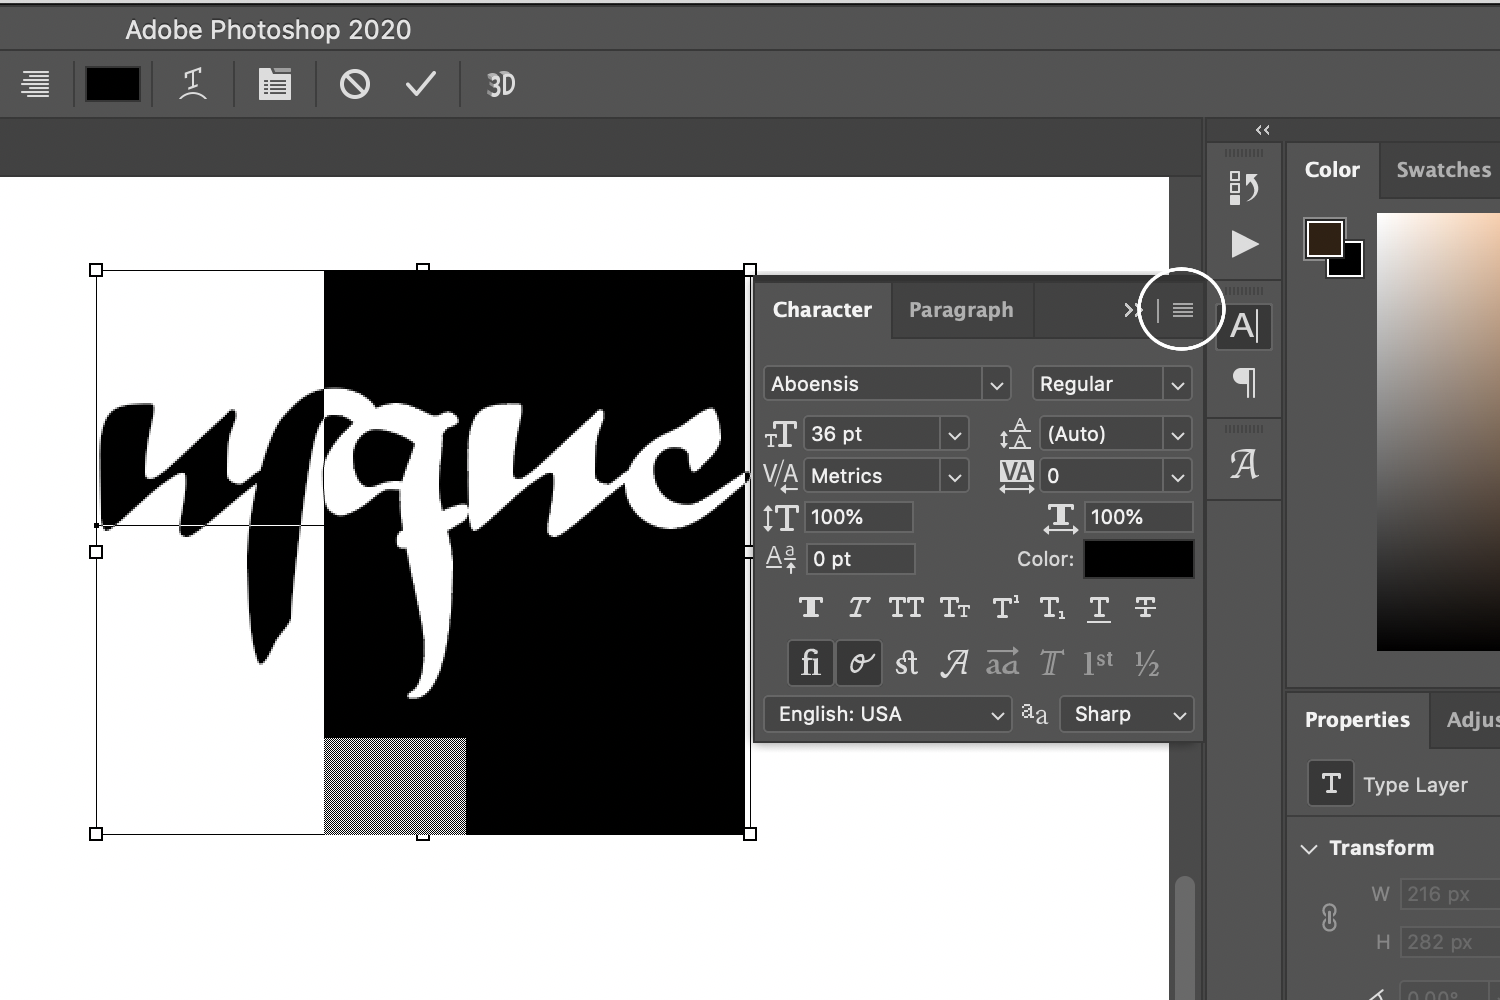
\includegraphics[width=8cm]{pics/photoshop-one.png} 
  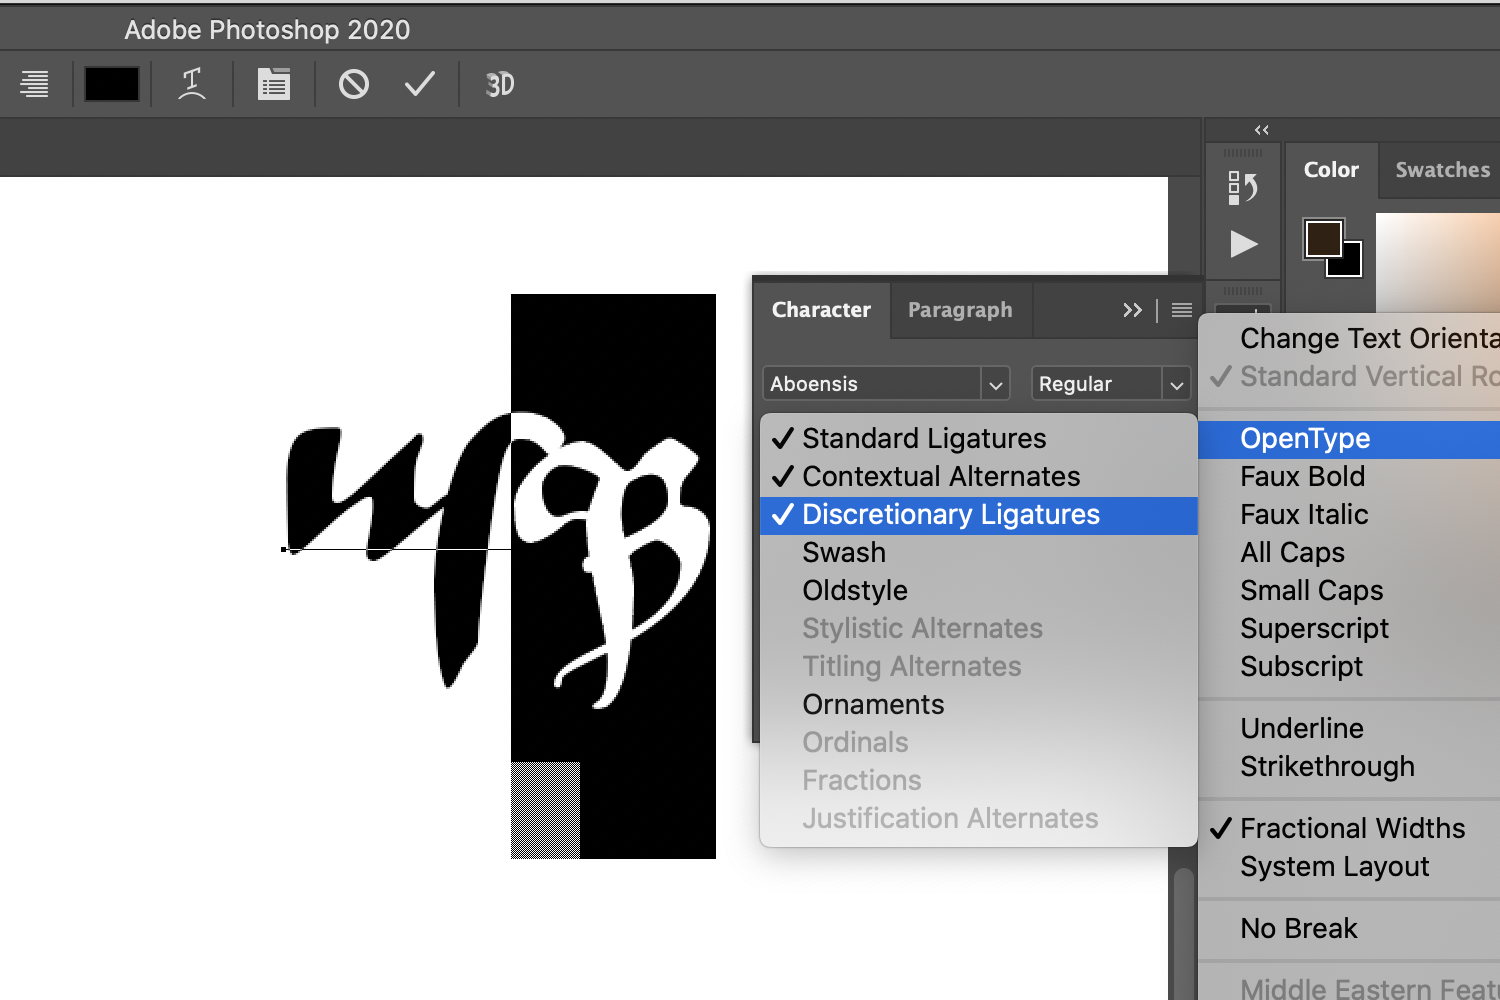
\includegraphics[width=8cm]{pics/photoshop-two.png}
  \caption{The OpenType menu in Photoshop}
  \label{fig_photoshop}
\end{figure}

\begin{figure}
  \centering
  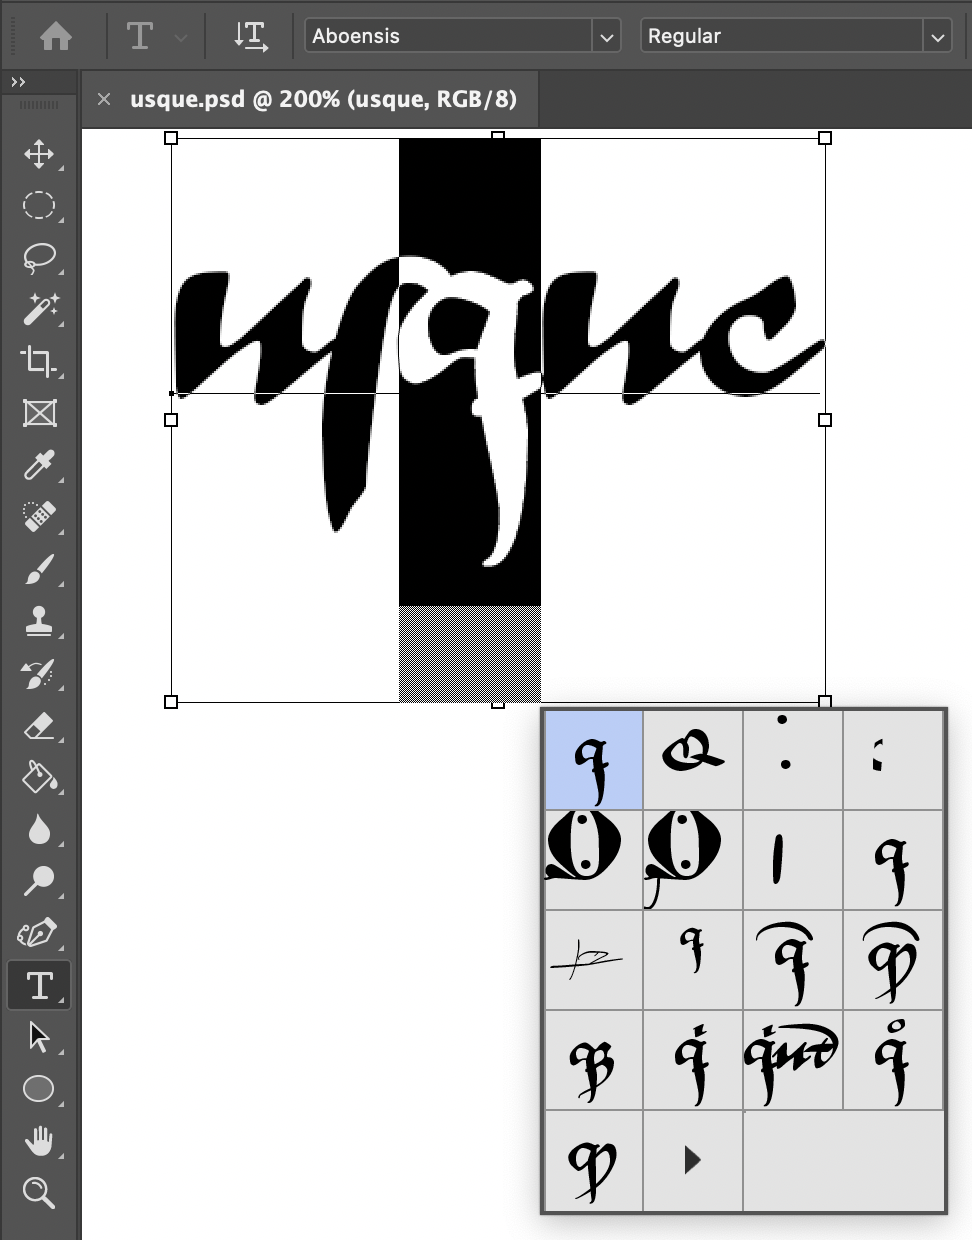
\includegraphics[width=6cm]{pics/photoshop-alternatives.png} 
  \caption{Selecting character variants in Photoshop}
  \label{fig_photoshop_2}
\end{figure}




\subsection{Open Font License v.1.1}


\Aboensis{} may be used and distributed under the conditions of the
Open Font License v.1.1. The full text of the license is at the end of
this document. It and answers to frequently asked questions about it
are available at \texttt{http://scripts.sil.org/OFL}. The most
important features of OFL are:
\begin{enumerate}
\item You may freely use the font in your documents, including
  embedding it in it.

\item You may freely give the font to whoever you want, but you should
  give the whole package (including the documentation files). You may
  also sell it as long as you comply with the few restrictions that
  are enumerated in the text of the license.

\item You may freely modify the font, but if you distribute the
  modified font you should give it a different name and release it
  under OFL.
\end{enumerate}


\subsection{Latex Project Public License version 1.3c} 

The documentation files (except for images showing original medieval
documents) and the LaTeX style file are distributed under the Latex
Project Public License (LPPL version 1.3c). The exact conditions of
the license are defined in the file \texttt{lppl.txt} that should be
included in the font package but is also available at
\texttt{http://www.latex-project.org/lppl.txt}.

The terms of LPPL are similar to those of the OFL. The short and
incomplete version is:
\begin{enumerate}
\item You may freely use the files however you want. 

\item You may freely distribute the package in its original form. 

\item If you modify the files, you may distribute them but you must
  document what changes you have made in the files, make it clear that
  the changed version is not the original, and distribute either the
  original version or information on how it can be obtained with it.
\end{enumerate}

\subsection{Creative Commons Attribution 4.0 International License}

Most of the images that show reproductions original medieval documents
are copyrighted under the Creative Commons Attribution 4.0
International License (CC BY 4.0) by the institutions that digitized
them. The list of copyright holders is on pages
\pageref{image_license_start}–\pageref{image_license_end}.

The exact conditions of the license are defined in the file
\texttt{ccby4.txt} that should be included in the font package but the
text is also available at
\begin{center}
\texttt{https://creativecommons.org/licenses/by/4.0/}.  
\end{center}
The short and incomplete version of the license is that you are free
to:
\begin{enumerate}
\item \textbf{Share} — copy and redistribute the material in any
  medium or format  
\item \textbf{Adapt} — remix, transform, and build upon the material
for any purpose, even commercially. 
\end{enumerate}
under the following terms:
\begin{enumerate}
\item \textbf{Attribution} — You must give appropriate credit, provide
  a link to the license, and indicate if changes were made. You may do
  so in any reasonable manner, but not in any way that suggests the
  licensor endorses you or your use
\item \textbf{No additional restrictions} — You may not apply legal
  terms or technological measures that legally restrict others from
  doing anything the license permits.  
\end{enumerate}

\emph{All images in this document that are licensed under CC BY 4.0
  have been cropped from larger originals, including those that show
  the complete text of the document.}



\section{Historical background}

\subsection{Codex Aboensis}

The \emph{Codex Aboensis} (\emph{Cod. Holm. B 172}) is a
richly-illustrated late-medieval book that is currently held in the
Swedish National Archives. It is known also by the name \emph{Codex
  Kalmar} as it was for a time stored in a school library in Chalmers
before it was donated to the Archives in 1884.

The main content of the book is the \emph{Law of the Realm of King
  Magnus Eriksson} that has been supplemented by the \emph{Church Law
  of Uppland}, the \emph{Manor Justice of Magnus Eriksson}, and the
\emph{Ledung code of Uppland} that decrees how the coastal fleet was
organized.

The book is connected to Finland and the city Turku (\emph{Abo} in
Latin) in several ways. The most notable is that the book starts with
an ecclestical calendar of the Turku diocese. The other is that it is
known to have been in Finland for most of the 16th
century.\footnote{Its front and back leaves also contain material
  written by the hand of Micael Agricola (1510–57) who was the main
  Lutheran reformer of Finland.} However, the calendar is older than
the bulk of the text and dates from the latter half of the 14th
century with some modifications made around the beginning of the
1400s.

The most striking feature of the manuscript are the large illuminated
initials that start almost every page. The images were drawn by the
original scribe, and he likely drew himself in one of them. The folio
78v shows a man in tunic, red hose and red hat holding a speech scroll
that declares him to be the master of books (figure \ref{fig_master}).
The page initials usually start mid-sentence. 

\begin{figure}
  \centering
  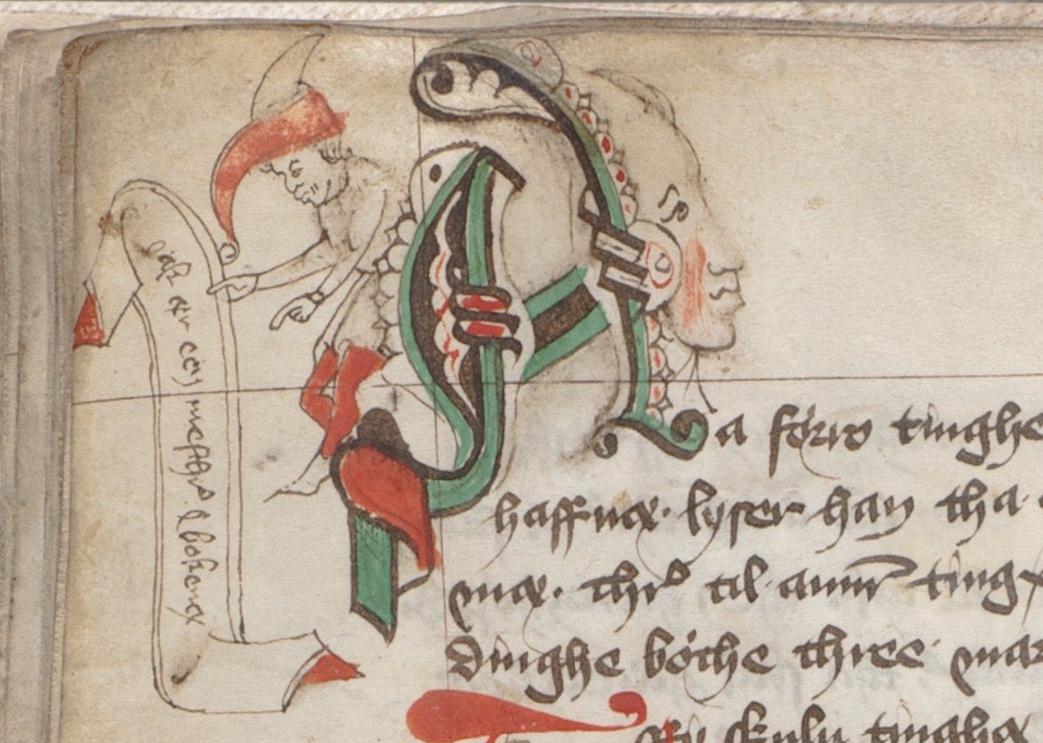
\includegraphics[width=10cm]{pics/aboensis-78v.png}
  \caption{Possibly the scribe of \emph{Codex Aboensis} himself. The
    speech scroll reads: \emph{jak är een mesther i bokenä} which
    translates to \emph{I am a master of books}. f.78v}
  \label{fig_master}
\end{figure}

\begin{figure}
  \centering
  \subfigure[A fox preaching to geese, f.18v]{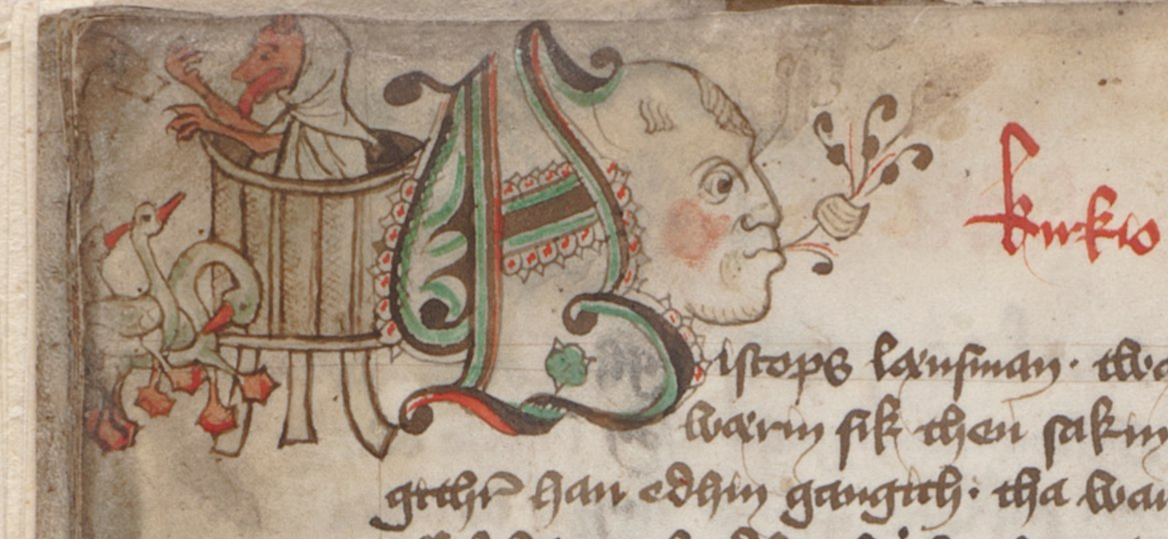
\includegraphics[width=6cm]{pics/aboensis-18v.png}}
  \subfigure[A cleric carrying a woman, f.30v]{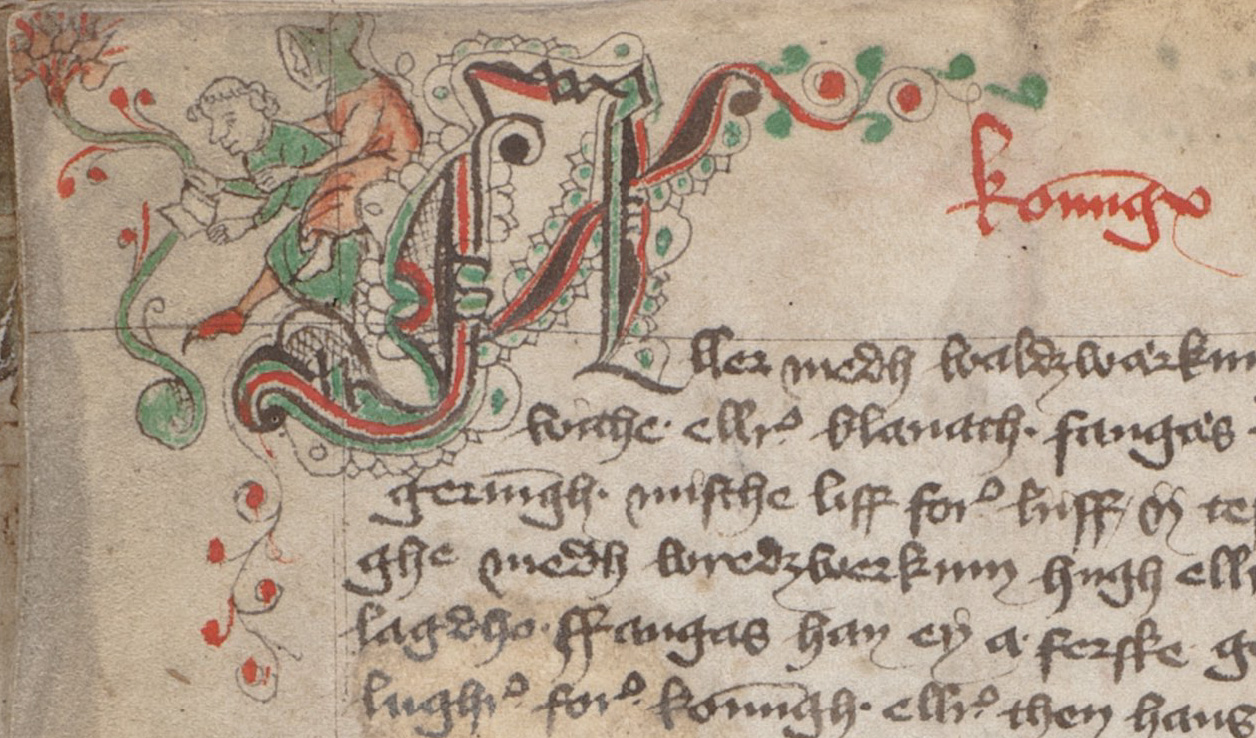
\includegraphics[width=6cm]{pics/aboensis-30v.jpg}}
  \subfigure[A hare playing bagpipes, f.37v]{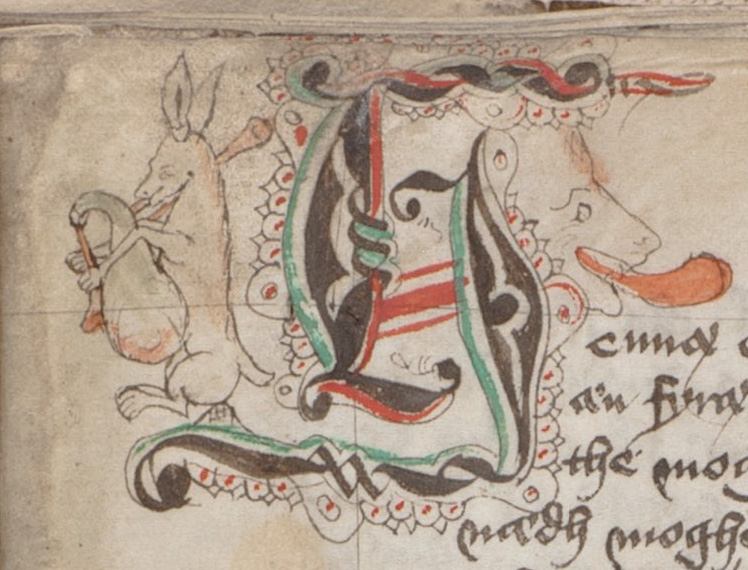
\includegraphics[width=6cm]{pics/aboensis-37v.jpg}}
  \subfigure[A man carrying an ale barrel. The speech scroll reads \emph{wiliom wi dricka}, that is \emph{now we drink}. f.38v]{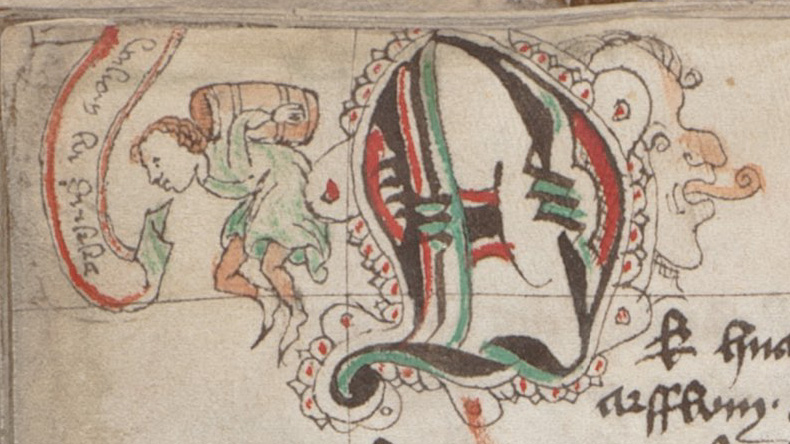
\includegraphics[width=6cm]{pics/aboensis-38v.jpg}}
  \subfigure[Ivan Lejonriddaren kills a dragon, f.39r]{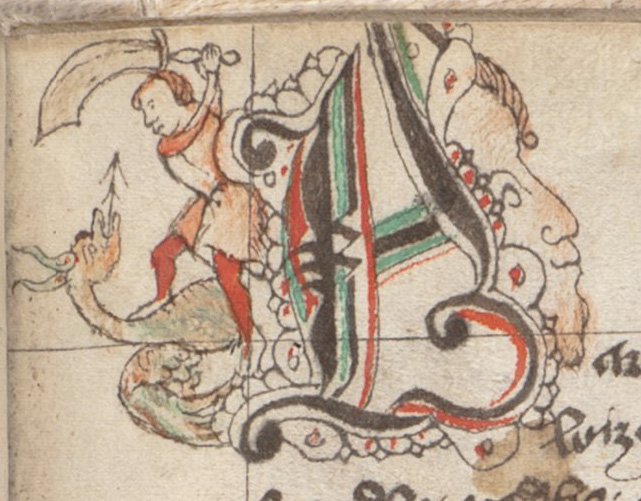
\includegraphics[width=6cm]{pics/aboensis-39r.jpg}}
  \subfigure[Ivan Lejonriddaren riding his lion, f.39v]{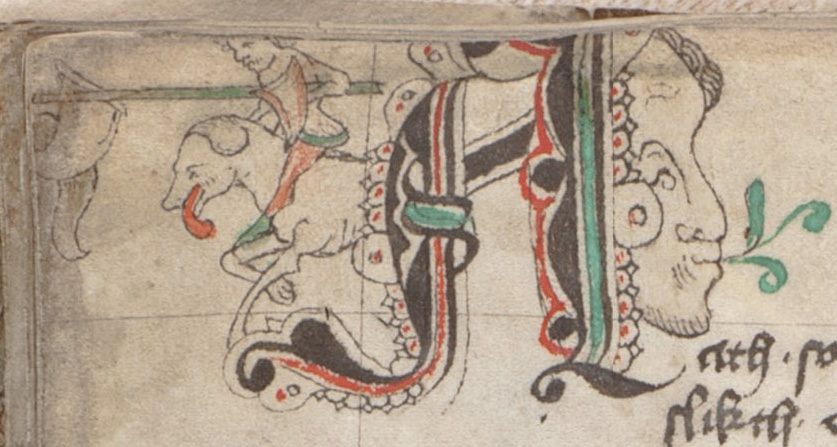
\includegraphics[width=6cm]{pics/aboensis-39v.jpg}}
  \caption{Picture samples from \emph{Codex Aboensis}.}
  \label{fig_samples}
\end{figure}

Most but by no means all of the images are at least loosely related to
the text where they occur. The figure \ref{fig_samples} shows a few
more samples.

{\renewcommand{\theenumi}{\alph{enumi}}
\begin{enumerate}
\item A fox preaching to geese from a transportable pulpit of the type
  that friars used. This is in a section that defines how the bishop
  should inspect a church that is suspected to have been desacrated.
\item A cleric carrying a woman. This is not directly related to text
  that is about punishments for fighting in a tavern. 
\item A hare playing bagpipes. This is probably connected to the
  mention that a bride of a wedding may not donate wedding cloths to
  musicians but only to a church or a monastery.
\item A man carrying an ale barrel while saying: "Now we drink". This
  is in a section that gives rules on gifts given on the morning after
  a wedding and it may refer to custom of drinking a toast when it
  happened.
\item This and the next picture show probably scenes from the story of
  Ivan Lejonriddare, Ivan the Lion Knight who killed a dragon and
  befriended a lion that became his mount. The connection to the text
  is that the text describes complex inheritance cases and Ivan of the
  story was involved in one himself.
\end{enumerate}}

There have been differing opinons on where and when the manuscript was
written. Paleographical details place it in the first half of the 15th
century. The two main opinions have been Uppland in Sweden and
Turku-Naantali region in Finland, both areas being proposed on
linguistic basis.

The most recent paleographic analysis by Per-Axel Wiktorsson suggests
that the main body of text was written by an anonymous scribe who was
active in Stockholm between 1423–36. The scribe was connected to Bengt
Jönsson Oxenstierna (c.1390– c.1450) who was one of the
highest-ranking noblemen in Sweden, a Privy Council member who served
as a co-regent in 1448. Wiktorsson's theory is that Bengt Jönsson
commisioned the book in mid-1430s as a preparation for his bid to
become the \emph{lagman} (Lord Justice) of Uppland. He recived the
position in 1439.

\begin{figure}
  \centering
  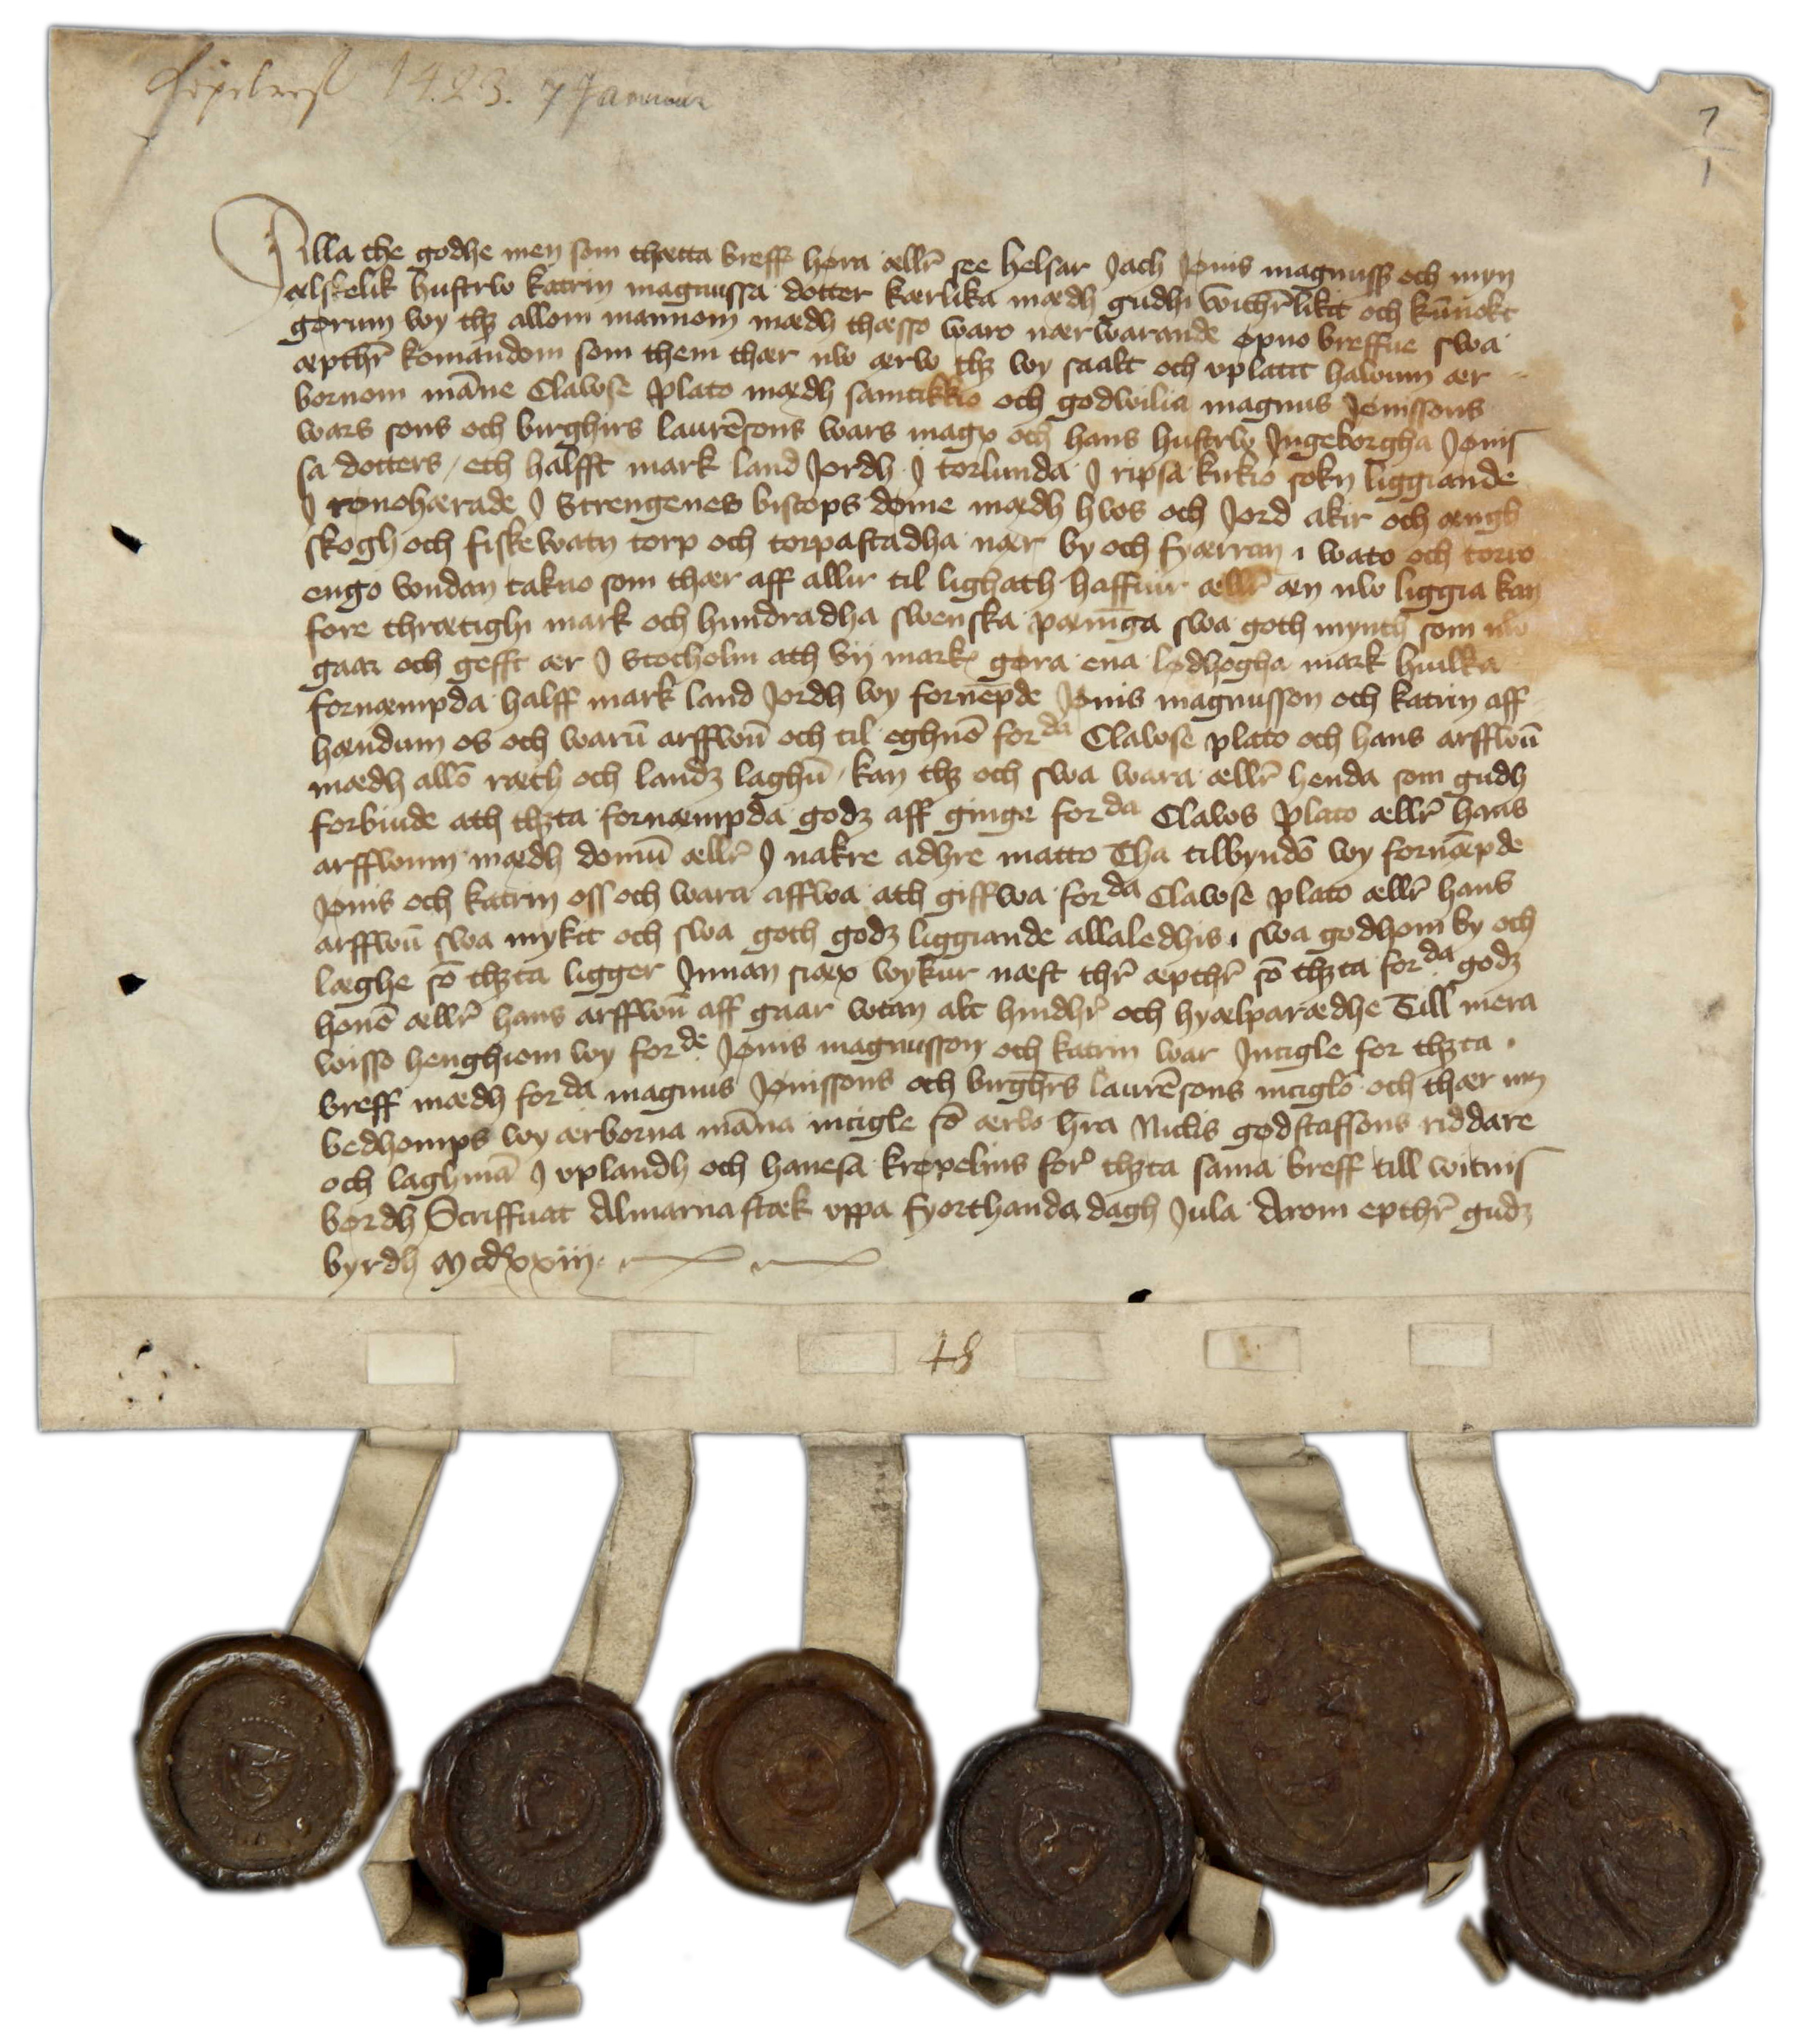
\includegraphics[width=13.5cm]{pics/SDHK20000.jpg}
  \caption{A sales deed dated 1.7.1423 at Almarestäk castle.
    Wiktorsson identified it as being by the same scribe that copied
    \emph{Codex Aboensis}, SDHK 20000.}\label{fig_alamarestak}
\end{figure}


The manuscript contains 123 parchment folios that are sandwiched
between blocks of paper at front and end. First six parchment folios
contain the calendar and the rest make up the legal text. The folios
are $24 \times 16.5$ cm in size where the text area is $16.5 \times
11.5$ cm. There are 25–29 lines of text per page where 27 is the most
common number. The pages in the front and at the end contain later
writing. For example, the end contains astrological material written
in hand of Micael Agricola (figure \ref{fig_astrology}).

The \emph{Realm of the Land} is written in a cursive script of the
kind that was in wide use in Sweden around the time. The scribe used
very clear and careful hand suitable for a high-profile manuscript or
an important document.


\begin{figure}
  \centering
  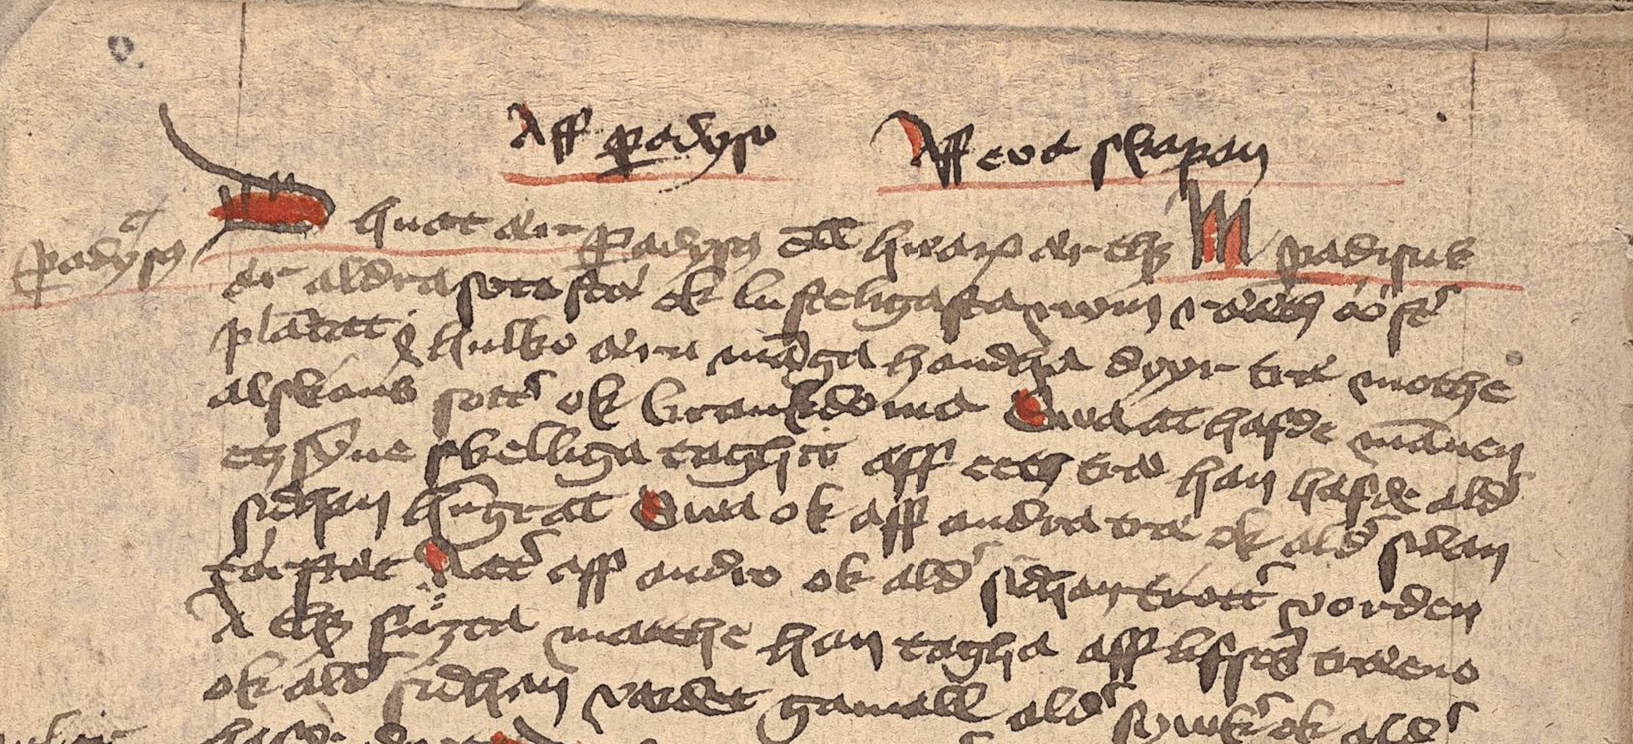
\includegraphics[width=12cm]{pics/budde-9v.png}
  \caption{Sample from \emph{Jöns Budde's Book} that shows a less
    clear cursive text from slightly later period c.1490 (\emph{Codex
      HS A 58, f.9v}) }
  \label{fig_jons_budde}
\end{figure}





\begin{figure}
  \centering
  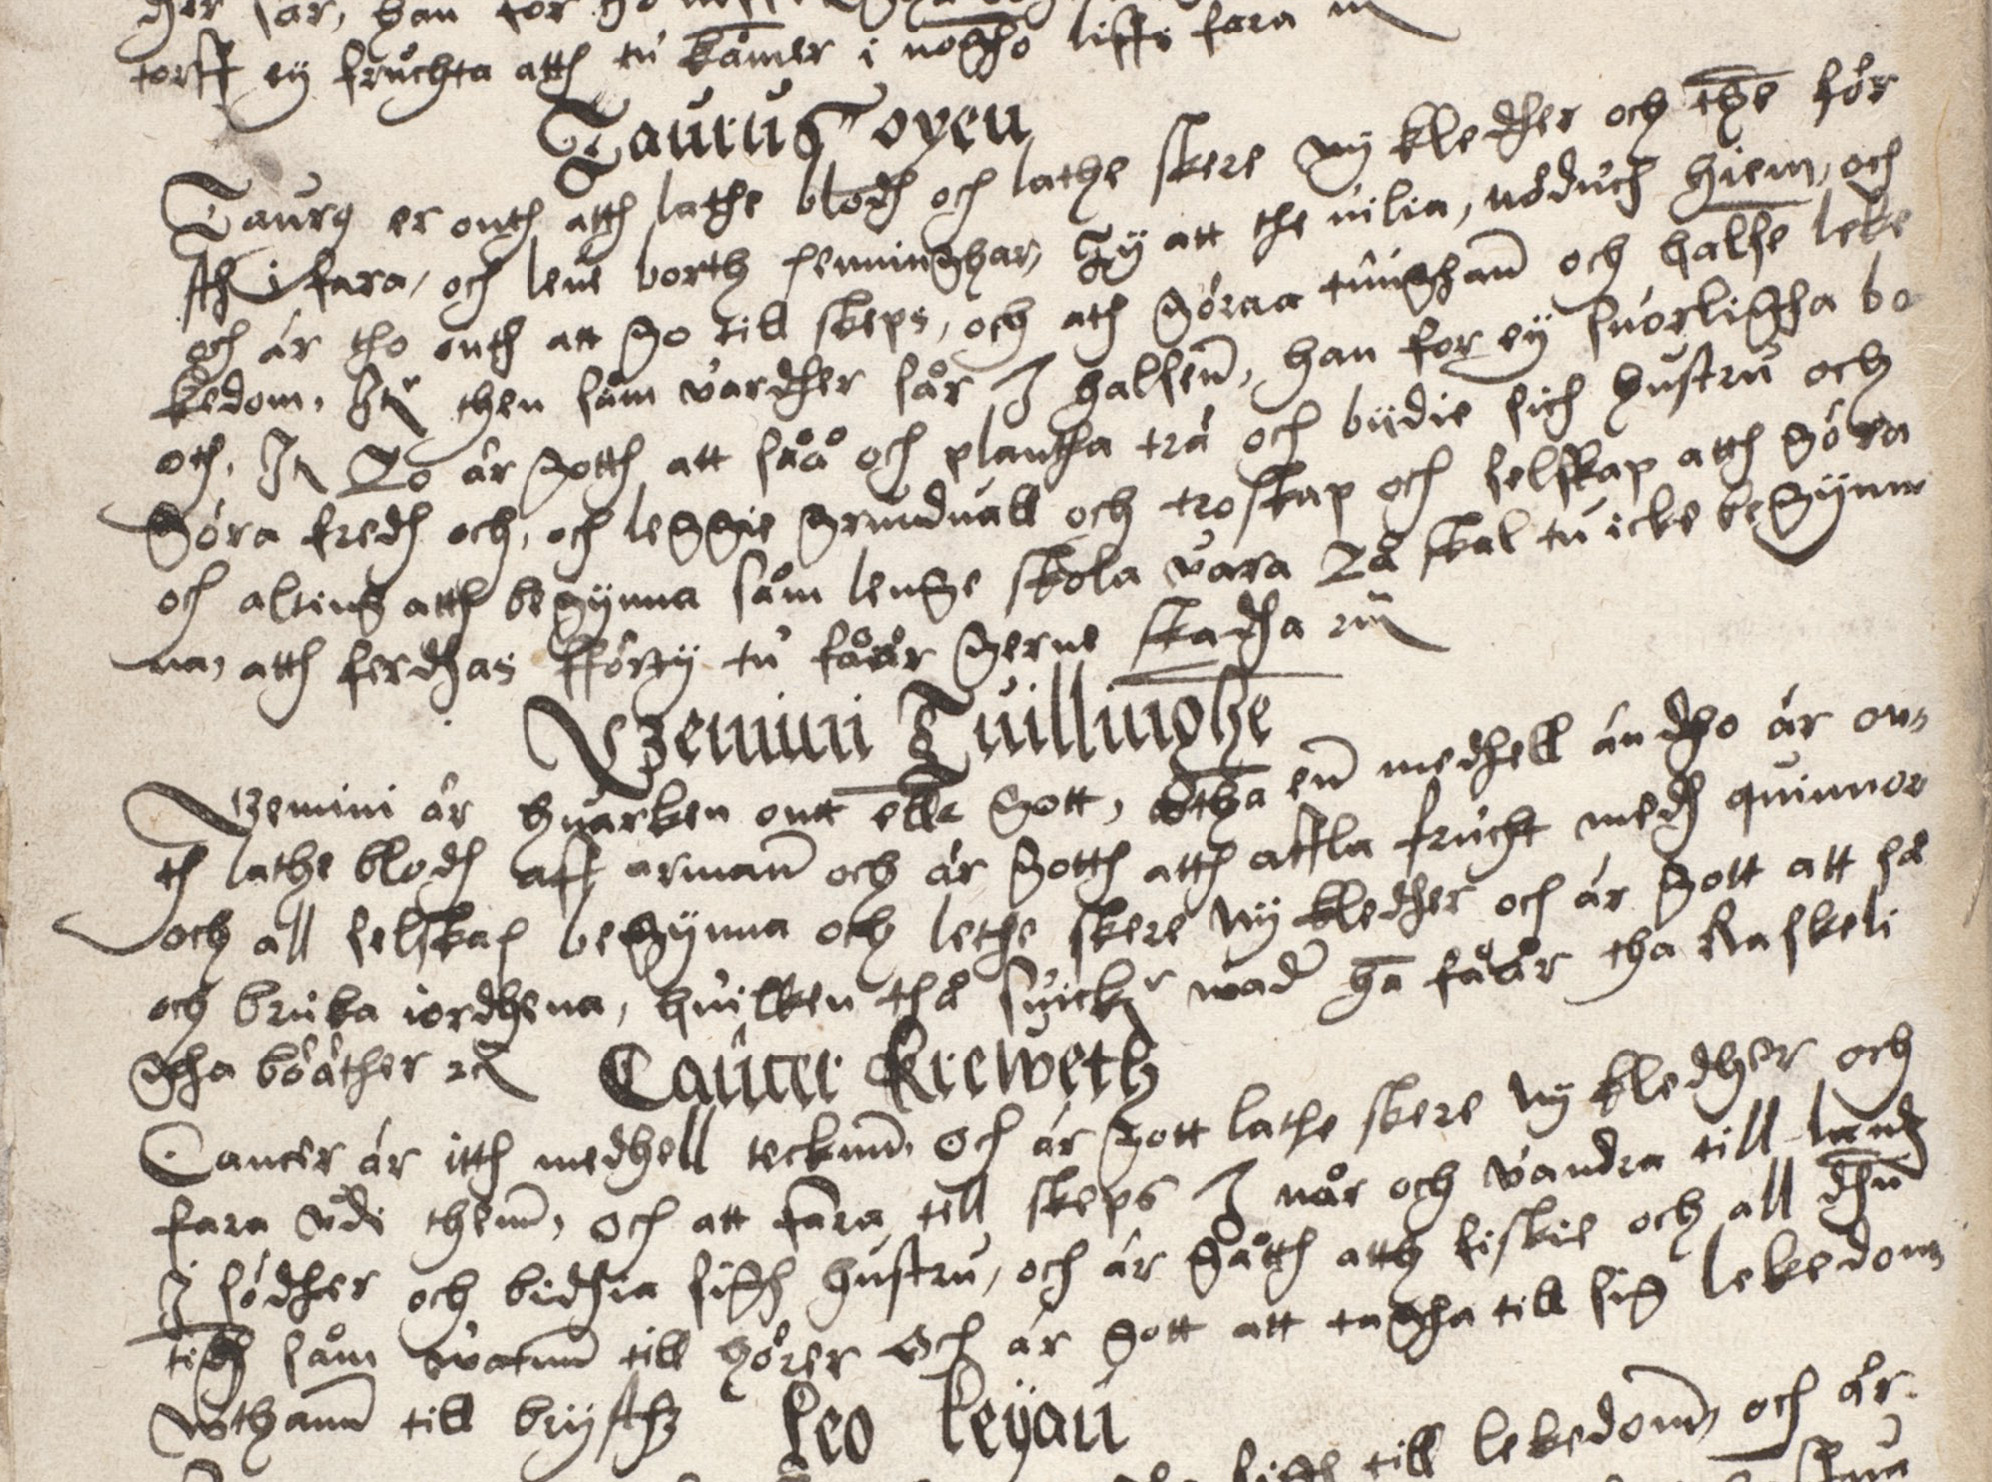
\includegraphics[width=12cm]{pics/aboensis-e14v.jpg}
  \caption{A part of an astrological text written by Michael Agricola
    on the end pages of \emph{Codex Aboensis} (f14v)}
  \label{fig_astrology}
\end{figure}



\subsection{King Magnus Eriksson}

Magnus Eriksson was born in 1316. At the time the situation in Sweden
was tense. King Birger Magnusson had fought a bitter civil war against
his brothers Erik and Valdemar, Dukes of Södermanland and Finland, and
now there was an uneasy peace. Magnus was the first son of Duke Erik
and Ingeborg of Norway, who was the daughter of King Haakon Magnusson
of Norway. 

The truce was broken in 1317 when Birger captured his brothers during
a celebration in Nyköping and had them killed. According to the
\emph{Eric Chronicle} they were starved to death. The supporters of
the dukes raised a rebellion and forced Birger to exile to Denmark
where he died in 1321. The 3-year old Magnus was elected as king at
the Stones of Mora in 1319. A few months later he was declared the
hereditary King of Norway after the death of his grandfather. 

Magnus was crowned in 1331 after a 12-year regency and he became the
longest-reigning King of Sweden before the currently reigning Karl XVI
Gustav. His rule as a King of Norway didn't last as long. The
Norwegian nobles were not enthuastic about union of Norway and Sweden
and after a series of revolts they came to a settlement in 1343 where
Magnus abdicated the throne in favour of his younger song Haakon.
Magnus continued to be the regent until Haakon came of age in 1355.

In Sweden Magnus started a legislative reform. In the 1330s he
insituted his \emph{Manor Justice}, the \emph{The Law of the Realm}
that was intended to become the unified law in the whole country was
written in 1340s and in the next decade he followed it with \emph{The
  Law of the Towns}. In practice these two law collections did not
come to force immediately and some areas used their old laws for the
next century.

In 1360 King Valdemar IV of Denmark attacked Magnus's lands and
reconquered Scania that Magnus had held for a few decades. The next
year he conquered the island of Gotland. The decicively lost war
triggered a rebellion in Sweden that Magnus vanquished. A few of the
rebels, led by Bo Jonsson Grip went to the court of Albrecht of
Mecklenburg and offered the crown to him. With the support of the
Hanseatic league Albrecht conquered central parts of Sweden and he was
crowned a king in 1364.

After that there was a civil war between supporters of Magnus and
Albrecht that lasted for almost eight years. Magnus himself was
captured at the Battle of Gataskogen in 1365 and had to spend years in
prison. In there was a peace agreement where Magnus agreed to leave
the kingdom for Albrecht and to go to exile in Norway where he died in
a shipwreck two years later in 1374.


\subsection{Swedish laws}

At the beginning of the 14th century there were several provincial law
codes in effect in Sweden. The contents of nine of them are known
completely or partially, but there may have been others that are not
mentioned in sources. For example, it is not known what law code or
codes were followed in Finland. There are a few references to the
Hälsinge Law but there are also vague references to "laws and customs
of the land" that may refer to local law codes. The codes were divided
into two basic groups: \emph{Göta Laws}\footnote{Including the Older
  and Younger Västgöta, the Östgöta, and the Småland Laws.} were
followed in the Western provinces and \emph{Svea Laws}\footnote{The
  Uppland, Dala, Västmanna, Hälsinge and Södermanna Laws.} of Eastern
Sweden. The Scania Laws are nowdays usually grouped with the Danish
medieval laws because Scania belonged to the Danish crown for almost
the whole middle ages.

The development of the laws is not clear. It is probable that at least
some of them existed orally before they were written down. The oldest
legal manuscripts contain The Older Västgöta Law and they date to the
early 13th century.

Magnus Eriksson's \emph{The Laws of the Realm} contains 14 chapters
that are called \emph{balke}. The term translates literally to
\emph{beam}. Its etymology is not certain, but it may have been
intended to convey the meaning of support. 


\paragraph {Konungs balker – King's Beam} \mbox{}\\

The \emph{Konungs balker} starts with laws about the election and
coronation of the king as well as giving the text of the regnal oath
that limited his powers. Then it describes the rules of the armed
service for noblemen. The third main part of the \emph{balke} gives
rules on how king's court work. In addition to these main parts there
are regulations on various matters. For example, the section 23
decrees that taverns should be established along the main roads of the
kingdom and gives rules for their operation.


\paragraph {Giffto balken – Wedding Beam} \mbox{}\\

The \emph{Giffto balken} establishes regulations on the marriage. It
defines when an engagement and a marriage are legal and how dowry and
morning gift\footnote{A gift given by the husband to his new wife on
  the first morning of their marriage.} are given. It also establishes
limits on the gifts and for the number of guests in a wedding. The
limit on the guests were probably intended to prevent large gatherings
that could be used as cover for mustering forces for a rebellion.

\paragraph {Ärffdha balker – Inheritance Beam} \mbox{}\\

The \emph{Ärffdhe balker} is a short code that establishes rules for
dividing the inheritance. The basic principles are that the
inheritance goes to closest relatives and that a daughter inherits
half as much as her brothers. A special emphasis is placed on ensuring
that no one can inherit a person they have killed.


\paragraph {Jordha balker – Land Beam} \mbox{}\\

The \emph{Jordha balker} is a long code giving rules on how land
properties work. Land holdings were divided into two classes:
\emph{inherited} and \emph{bought}. The general rule was that a person
could freely sell land that they had bought, but inherited land needed
to be first offered for the relatives to buy. The law also decreed
that there needed to be a written sales for every land sale. The balk
contains also regulations for tenant farmers who rented the land that
they farmed.

\paragraph {Bygningah balker – Building Beam} \mbox{}\\

The \emph{Bygningah balke} contains mostly rules on how villages work:
how the building plots are arranged and how common fields and meadows
were divided beween farms. Because each farm had a share on each
field, the whole village had to coordinate their work. Other parts of
the balk describe how servants are hired, how borders between villages
are marked, and how mills and bridges are built, among a few other
things.

\paragraph {Köpmala balker – Trade Beam} \mbox{}\\


The \emph{Köpmala balker} is a short code that contains regulations on
how trades are legally made. It establishes penalties for selling fake
or stolen things as well as regulates how loans are given and
guaranteed. 


\paragraph {Thingmaala balker – Court Beam} \mbox{}\\

The \emph{thing} was an assembly of men of a given area that
functioned also as the court of justice. The \emph{Thingmaala balker}
decrees how courts are held. It starts by giving rules on how
\emph{lagmans} and judges are selected and then establishes how and
when the \emph{things} were held. Each district had three sessions
each year (from Epiphany to Ash Wednesday, from June 17 to July 39,
and from St Michael's day to the First Advent) and during the sessions
the court sat on one day a week.

Sworn oaths were the integral part of court proceedings. For each
possible dispute the rules said whether the plaintiff, the defendant,
or the jury needed to swear the oath and how many men were necessary
for it.\footnote{\emph{Men} is literal here because women were not
  allowed to swear an oath at a \emph{thing}.} It was not allowed to
counter an oath with another oath and no one was allowed to swear an
oath alone but instead needed to find a number of co-swearers to go
along him. Very simple cases needed only an oath of two men, serious
cases needed 12.

The balk also establishes rules on how fines could be collected and
decreed forced labour for those who couldn't pay them.

\paragraph {Edzöris balker – Peace Oath Beam} \mbox{}\\

The peace oaths were laws that gave special protection to different
areas of life. They originated in Germany and the first mentions for
them in Sweden come from the 12th century. They came to prominence
during the reign of King Magnus Ladulås (reigned 1275–90). The penalty
for breaking them was usually outlawry but doubling the normal fines
was used for less serious offences. Because children and women
couldn't be outlawed, they also could not be punished for breaking the
peace oath.

The \emph{Edzöris balker} gave protection to:

\begin{itemize}
\item Homes: attacking someone in his home broke the oath;
\item Justice: exacting a revenge on the other participant of a trial
  after the case was settled in the court broke the oath as did
  participating in a blood feud;
\item Women: raping a woman broke the oath;
\item Church: wounding or killing people in church or who were
  traveling to or from church broke the oath;
\item Court: wounding or killing people at court or who were traveling
  to or from it broke the oath.
\item Mutilation: mutilating someone by cutting of their body parts
  broke the oath;
\item Fieldwork: attacking someone who was working on fields carried a
  penalty of double fines but not outlawry.
\end{itemize}

Attempts were not criminalized under the beam. Trying to attack
someone going to church but failing the attempt was explicitly said to
not break the oath.

\paragraph {Högmalis balker – Capital Matters Beam} \mbox{}\\

The \emph{Högmalis balker} lists crimes for which the sentence was
death on a wheel for men or stoning for women.

The crimes were secret murder where the body was hidden, killing one's
own child or parent, bigamy, killing someone with witchcraft or
poison, armed rebellion, helping an invading foreign army, killing
one's liege lord, and arsony.

The final paragraph of the law decrees that an attempt to harm someone
with witchcraft or poison was punished by a fine of 40 marks.


\paragraph {Draapmala balker medh wiliä – Murder Beam} \mbox{}\\

There are two \emph{balker} about killings. The \emph{Draapmala balker
  medh wiliä} handles the cases where the killing was intentional.
This has some overlap with the \emph{Högmalis balker}.

In contrast to modern laws, the punishment for murder depended on when
the criminal was caught if it was not a secret murder. If the criminal
was caught within a day of the murder, then the punishment was death,
but if captured later, then the punishment was a fine that was
typically 40 marks but in some cases it could be smaller or larger.
The fine was divided into three parts, one third going to the
plaintiff, one third to the king, and one third to the parish. In case
the fine was larger than 40 marks, the shares of king and the parish
were capped at 13 marks 8 öres that corresponded to their share of the
40 marks.

Magnus Eriksson's \emph{The Laws of the Realm} have still vestiges of
old feuding culture. If a close relative of a murder victim killed the
killer within one day of the murder, he could not get a death sentence
even if caught immediately afterwards and he would need to pay only
the king and the parish thirds of the fine.

The balk also gives rules on how an exiled killer can get a safe
conduct to king's court and obtain reconciliation.

\paragraph {Draapmala balker medh wadha – Manslaughter Beam} \mbox{}\\

The \emph{Draapmala balker medh wadha} considers accidental killings.
It gives rules on when a killing is counted as accidental and
specifies fines for different causes of death. The general rule is
that when the killer has taken some active action that causes death,
the fine is 9 marks divided in three, and if the death is because the
defendant has neglected to do something or if the victim was an active
participant of whatever caused the death, then the fine is four and
half marks.

\paragraph {Saramalä balker medh wiliä – Intentional Wounding Beam}
\mbox{}\\

There are also two \emph{balker} about woundings and \emph{Saramalä
  balker medh wiliä} is about cases where someone intended to cause an
injury. The balk lists different types of injuries and gives
compensations and fines that needed to be paid for them. The
compensation went fully to the injured party while the fine was
divided in three parts just like the fines for murders were. 

For example, cutting a hand away called for compensation of 12 marks
and a fine of 20 marks. Cutting a thumb had a nine mark compensation
and 12 mark fine.

\paragraph {Saramalä balker medh wadha – Accidental Wounding Beam}
\mbox{}\\

The second wounding balk is about accidental woundings. It defines
when an injury is an accident and enumerates the compensations. In
general, the compensations were much smaller than for the intentional
cases. For example, accidentally causing the loss of a thumb called
for 12 öres compensation and 12 öres fines.

The \emph{Saramalä balker medh wadha} considers accidental injuries. 

\paragraph {Thiuffua balker – Thief Beam} \mbox{}\\

The \emph{Thiuffa balker} decrees punishments for thieves. As with the
case of murders, the punishment for thieves differed based on whether
they were caught in act or later. A thief who stole property worth of
half a mark or more who was caught in act would be hanged but if
caught later the punishment would be a fine of 40 marks and they would
need to pay the value of the goods. If the stolen property was worth
between 3 and 4 öres the punishment was flogging and cutting of ears
if caught in act or nine marks fine if not. If the value was between 2
and 3 öres, it was flogging and losing one ear or six marks fine, and
smaller thefts if was flogging or a fine of three marks.

The balk also gives rules how home inspections could be made to find
stolen goods and how someone who found lost property should act to
avoid been accused of thievery.


\paragraph {Gardz rättir – Manor Justice} \mbox{}\\

The \emph{Gards rättir} is a law for royal manors and the king's army
and its last section permits the lords of the Privy Council to apply
it also for their manors. In \emph{Codex Aboensis} it comes in the
middle of the \emph{Law of the Realm} between \emph{Konungs balker}
and \emph{Giffto balken}. This was the earliest law that Magnus
Eriksson enacted during his reign.

The law decrees punishments for various crimes. In contrast to the
common law, violent crimes are punished by corporal punishment instead
of fines. This is probably because soldiers and servants would not be
able to pay fines.


\paragraph{Kyrko balker – Church Beam}

The \emph{Kyrko balker} of provincial laws established the
organization of parish churches in Sweden. They originated during time
when canon law was not yet fully established. By Magnus Eriksson's
time the church was adamant that secular law should have nothing to do
with any matters relating to the church. This is almost certainly the
reason why Magnus didn't include \emph{Kyrko balker} in his laws.
Instead, the old provincial law balks were used in conjunction with
the new code.

\emph{Codex Aboensis} contains the \emph{Kyrko balker} of the Uppland
law. In addition of decreeing how the parishes work, it also contains
statutes about moral crimes.


\paragraph{Ledung rules}

The ledung institution was established near the end of the Viking age.
Its aim was to organize a semi-permanent navy. Each province was
responsible for providing a set number of ships and their crews and
provisions when king called for it. By Magnus Eriksson's time the
custom was antiquated enough that he didn't include it in the laws,
but \emph{Codex Aboensis} contains the ledung rules from the Uppland
provincial law.


\subsection{The Black Book of Abo Cathedral}

The other main source for charaters in \Aboensis{} is \emph{Registrum
  ecclesia Aboensis} or \emph{The Black Book of Abo Cathedral} that is
a cartulary originally compiled in the 1470s and new documents were
appended to it until 1515. The oldest documents that were copied into
it date from 1229 and the latest are from 1515. The most probable date
for when it was started is 1474 when the chancellary of the diocese
was was reformed.

The first Swedish cartulary was the Uppsala Archdiocese
\emph{Registrum} that was started in 1344 and the cartularies of other
diacoses followed its example. 

The book is about the size of modern A4 the leaves being $28.5 \times
21$ cm in size. There are 329 paper quarto folios\footnote{About 1/3
  of the folios are left empty.} in it. The paper block is protected
by two sheets of vellum that have been added to the front sometime
after the reformation.

The \emph{Black Book} contains copies of 727 documents that are
arranged by the subject and not chronologically. The book starts with
an index of the documents that were copied prior to 1486. Most of the
documents relate to the possessions of the cathedral and their
distribution between different \emph{tables} of the chapter. When
Reinhald Hausen published its contents in the early 20th century he
moved the documents to chronological order to make searching for them
easier.


\section{Typesetting Medieval Cursive}

This section gives a general view on using \Aboensis{} to write
medieval cursive, and the next section will give specific instructions
of using the LaTeX style file \package{aboensis.sty}. As a general
note I will use in the examples the letters \emph{ä} and \emph{ö} even
though it would be more accurate to use \emph{æ} and \emph{ø}. The
font itself uses same symbols for both.

Medieval cursive writing differs from modern computer-generated text
in many ways. The most obvious differences are that many letters have
multiple variant forms that occur in different positions, there are
many abbreviations, and punctuation conventions are very different
from modern. The \Aboensis{} font is made with OpenType features that
automatically choose the correct letter variant in most cases, but
there are cases where manual adjustment is needed. Many of the
adjustments are necessary because of limitations of OpenType engines
as changing the set of active features often breaks the letter context
that the automation relies on.

The first thing to note is that many letters have specific initial and
final forms. The letter \emph{m} has also an additional isolated form.
The different forms of \emph{m} are:

\begin{center}
  \begin{tabular}{cccc}
    \sample{*m*} & \sample{m*} & \sample{*m} & \sample{m}
    \\ 
    Normal & Initial & Final & Isolated \\
  \end{tabular}
\end{center}

For example, the word \emph{non} is written as:
\begin{center}
  \sample{non}
\end{center}

These forms are selected using the \texttt{calt} feature and the
feature should always be turned on with the font.

The two forms for letter \emph{s} are usually called \emph{long}
(\emph{ſ}) and \emph{short} \emph{s}. In gothic scripts the long
\emph{ſ} was used in initial and middle positions while the short
\emph{s} was used only in word-final positions:\footnote{This differs
  from later Fraktur convention where the short \emph{s} was used also
  at the end of syllables.}

\begin{center}
  \begin{tabular}{cc}
    \sample{*s*} & \sample{*s} \\
    Long & Short \\
  \end{tabular}
\end{center}

For example, the word \emph{suspicious} is written with long \emph{s}
in first two places and short \emph{s} at the end: 

\begin{center}
  \sample{suspicious}
\end{center}

If an \emph{s} occurred by itself, the Swedish texts usually wrote it
with a long \emph{s}. Some other areas preferred a short \emph{s} for
isolated forms.

A double \emph{s} is written either with two long \emph{s} or with the
\emph{ß} ligature.\footnote{Old Swedish often uses \emph{z} in place of
  \emph{e} after \emph{h} and \emph{s} so \sample{ß} can also mean
  \emph{se}.} The ligature is most often used at the end of the word:

\begin{center}
  \sample{mass} \\
  mass
\end{center}


The letter \emph{r} has also two forms, straight and round:

\begin{center}
  \begin{tabular}{cc}
    \sample{*r*} & \sample{*r:} \\
    Straight & Round \\
  \end{tabular}
\end{center}

The general rule for them in Gothic scripts is that the round \emph{r}
is used after 'round' letters and the straight \emph{r} in other
positions. What counts as a round letter varies between scripts. In
\emph{Codex Aboensis} the round letters are \emph{a}, \emph{e},
\emph{o}, and \emph{w}. The scribe was inconsistent about the letter
\emph{h} and there are some places with round \emph{r} after and
others with straight \emph{r}. The \texttt{calt} feature uses the
round \emph{r} with \emph{h}.\footnote{Most Gothic scripts use round
  \emph{r} after \emph{u} and \emph{p} but \emph{Codex Aboensis} uses
  straight.}

\begin{center}
  \sample{ar}  \sample{er*} \sample{or}  \sample{wr}  \sample{hr}  \sample{h*r}
\end{center}

A special feature in Swedish writing is that both \emph{er} and
\emph{re} at the end of the word are written with the same
\emph{re}-ligature:

\begin{center}
  \begin{tabular}{cc}
    \sample{riddare} & \sample{eller}  
    \\ 
    ridda\emph{re} & ell\emph{er}
  \end{tabular}
\end{center}

This usage is almost universal in \emph{Codex Aboensis} and very
common other Swedish texts, though many hands write the
\emph{re}-ligature as an superscript abbreviation mark:

\begin{center}
  \begin{tabular}{cc}
   \sample{ridd'a} & \sample{ell'} \\
   ridda\emph{re} & ell\emph{er}
  \end{tabular}
\end{center}

During the middle ages the symbols \emph{u} and \emph{v} were still
considered to be variant ways of writing the same letter. Both forms
were used for the vowel and consonant and there was no standard rule
for selecting between them. One reasonably common convention was that
initial positions were written with \emph{v} and other positions used
\emph{u}.\footnote{A peculiar Swedish custom was to write \emph{v} in
  the middle of a word as \emph{ffu} as in \sample{kloffue}.}

\begin{center}
  \begin{tabular}{cc}
      \sample{vniuerse} & \sample{seruus} \\
      universe & servus 
  \end{tabular}
\end{center}

The symbols \emph{i} and \emph{j} were also considered to be variant
forms of the same letter. The most typical use was that \emph{i} was
the default form but \emph{j} was used as in final positions and as
the last letter in a sequence of \emph{i} letters. The letter \emph{y}
was also used often for \emph{ii}.

\begin{center}
  \begin{tabular}{ccccc}
    \sample{xiii} &  \sample{wii} & \sample{wy} & \sample{liiff} & \sample{gudi} \\
    xiii & wii & wii &  liiff & gudi \\
  \end{tabular}
\end{center}


Gothic cursive tends to have the problem that sequences of \emph{m},
\emph{n}, \emph{u} and \emph{i} letters are quite unreadable. To make
these more legible, the font adds a dot over \emph{i} in a place where
it is next to a minim. For example, the word \emph{minimum} looks
without and with dots like:

\begin{center}
      \sample{m!i!n!i!m!u!m} \hspace{5mm} \sample{minimum}
\end{center}


Medieval scribes used many abbreviations in the texts. The most
commmon abbreviation was to leave out a \emph{m} or \emph{n} and mark
it by drawing a tilde over the previous letter:

\begin{center}
  \begin{tabular}{cc}
    \sample{nõ} & \sample{kon~ugx} \\
    no\emph{n} & konu\emph{n}gx 
  \end{tabular}
\end{center}

The tilde was also used to mark places where longer sequences of
letters were left out. There were several standard sigla for
abbreviating syllables. The abbreviations supported in 
\Aboensis{} are described in section \ref{sec_abbrs}. Few further examples
are:

\begin{center}
  \begin{tabular}{cccc}
    \sample{ecc~ia} & \sample{[prop]heta} &
    \sample{[quod]} & \sample{eo[rum]} \\
    ecc\emph{les}ia & \emph{pro}pheta & q\emph{uod} & eo\emph{rum} 
  \end{tabular}
\end{center}

Capital letters were used in a different way from modern. Proper nouns
were generally not capitalized and even God was usually written
lowercase. In \emph{Codex Aboensis} capital letters are mostly used to
mark beginning of paragraphs. In high-profile manuscripts capitals
were often marked by drawing a red strike through them.


\subsection{Creating highlighted capitals}\label{ssec_capitals}


The capital letters may have a highlight strike added to them. This is
implemented by writing three letters on top of each other: first the
capital itself, then a strike of the highlight color, and finally a
partial strike on a darker highlight color that covers the parts of
letters that are left under the strike. The two strikes are
interpreted as zero-width variant characters whose glyphs lie over the
previous character.  

\begin{center}
  \begin{tabular}{c@{ }c@{ }cc@{ }c@{ }cc@{ }c@{ }c}
    \fbox{\sample{A}} & + & \fbox{\sample{\abred{/A\phantom{A}}}} & 
    + & \fbox{\sample{\abdarkred{//A\phantom{A}}}}  & = & \fbox{\sample{\abcapital{A}}}\\
    A & &  {\color{abred}/A} & & {\color{abdarkred} //A} 
  \end{tabular}
\end{center}

The most common medieval highlight color was red but \emph{Codex
  Aboensis} contains also highlights in green. Figure
\ref{fig:predefined_colors} shows HTML hex code values for three
colors. The red and blue are taken from \emph{Missale Aboense}
facsimile while the green is from the digitized version of \emph{Codex
  Aboensis}. All values are in color space sRGB. These colors are also
defined in the LaTeX style file, the details are in section
\ref{ssec_color_model}.

\begin{figure}
  \centering
  \begin{tabular}{lccccc}
    Color &  Highlight & Dark highlight  & \package{xcolor} name \\
    \hline 
    Red & \fcolorbox{black}{abred}{\phantom{TEST}}  &
    \fcolorbox{black}{abdarkred}{\phantom{TEST}} & \package{abred}\\
    &  B1523E & 4D231C \\ 
    Green &\fcolorbox{black}{abgreen}{\phantom{TEST}}  &
    \fcolorbox{black}{abdarkgreen}{\phantom{TEST}} & \package{abgreen} \\
    & 62876E & 3F4D3C &  \\
    Blue &\fcolorbox{black}{abblue}{\phantom{TEST}}  &
    \fcolorbox{black}{abdarkblue}{\phantom{TEST}} & \package{abblue}\\     
    & 455F9B & 202F4D \\
  \end{tabular}

  \caption{Predefined highlighting colors}
  \label{fig:predefined_colors}
\end{figure}




\subsection{Selecting correct forms of letters}\label{ssec_correct_forms}

\Aboensis{} tries to automate selecting correct form a letter but that
is not always possible. Many OpenType rendering engines break
substitution context when the set of active features change. The most
obvious problem that it causes is that letters in the middle of word
get turned to initial forms. Using ligature substitutions for
inserting special characters helps to avoid most of these problems.
However, when parts of a word are in different colors, many font
engines insert a context break there. This happens most often when a
word starts with a highlighted capital letter. For example the
\emph{n} has the initial form in the following word: 
\begin{center}
  \sample{\abcapital{I}nter} \\
  Inter
\end{center}
There are two special ligature substitutions with symbols \emph{*} and
\emph{!}. Both of them are treated as zero-width letters when used
next to a letter. We can add either of them between \emph{I} and
\emph{n} to remove the initial form:
\begin{center}
  \sample{\abcapital{I}*nter} \\
  I*nter
\end{center}

The difference between \emph{*} and \emph{!} is in how they tie
surrounding letters together.  Several of the letters have two forms,
 normal and tailed, where tailed is used to connect the letter to the
 next letters that have beaks at the left edge. For example, the
 letter \emph{a} has the following forms: 
 \begin{center}
   \begin{tabular}{cccc}
     \scalebox{1.5}{\sample{a*}} & \scalebox{1.5}{\sample{a!}}  \\ 
     Normal & Tailed \\
   \end{tabular}
 \end{center}
 If there is a string \emph{ai} where the letters belong to different
 contexts, then the \emph{a} will have the wrong form and they do not
 tie together properly. Adding \emph{!} to the same context as
 \emph{a}  solves the issue
\begin{center}
  \begin{tabular}{cccc}
    \scalebox{1.5}{\sample{\abred{a}i*}} &  &
    \scalebox{1.5}{\sample{\abred{a!}i*}} \\
    {\color{abred}a}i & & {\color{abred}a!}i
  \end{tabular}
\end{center}
In practice, it is rare for a situation to crop out where \emph{!} is
necessary and you can almost always use \emph{*} to solve context
breaking problems.

The asterisk and exclamation mark can also be used to change a round
\emph{r} to straight or short \emph{s} to long if desired:

\begin{center}
  \begin{tabular}{cccc}
    \sample{or} & \sample{o*r} & \sample{is} & \sample{is*} \\
    or & o*r & is & is* 
  \end{tabular}
\end{center}

Conversely, a straight \emph{r} or long \emph{s} can be changed to
round \emph{r} or short \emph{s} by adding \emph{:} after them:

\begin{center}
  \begin{tabular}{cccc}
    \sample{br} & \sample{br:} & \sample{sa} & \sample{s:a} \\
    br & br: & sa & s:a
  \end{tabular}
\end{center}

Abbreviation symbols can be added to symbols by prefixing them with
\emph{~}, \emph{'}, and \emph{/}. Not all combinations exists. Most
lettes have one with a tilde, many have single quote ones but there
are only a few with a slash.\footnote{Note that the slash implements
  highlighting for capital letters.}

\begin{center}
  \begin{tabular}{cccc}
  \sample{~d} & \sample{'t} & \sample{/d} \\
  ~d & 't & /d
  \end{tabular}
\end{center}



\subsection{Lombard and cursive initials}\label{sec_initials}

The font has three sets of initials: two sets of Lombardian initials
and one set of cursive initials. Lombardian initials were used in
books and cursive initials were used for documents. All three sets can
be accessed either using ligature substitutions or by turning on
suitable opentype features, and there are also XeLaTeX macros for
inserting them. 

The kind of Lombardian initials that are included in the font were
most often used as two-line initials in books, but they may also be
used as three- or one-line size. Larger initials were usually more
elaborate than these. Figure \ref{fig:initial_sample} shows a typical
example for two-line initial use. A longer version of the text is in
section \ref{sec_noble_service}.

\begin{figure}
  \centering
  \begin{minipage}{10.5cm}
    {\fontspec{Aboensis}\fontsize{15}{20}\selectfont\raggedright
      \noindent\abstartchapter{I}{\abl{\abcapital{O}ca mies wapautta tacto hänen hyfuydhens, }}{%
        {\abl{\hbox{\kern6.5pt{}mikä hän on \abcapital{R}iddari taicka \abcapital{S}wenni, ei }}}}
      \abl{yctäken eroittadhen, hänen pitä hyfuydhens}}
    \end{minipage}
    \caption{Sample for typical Lombardic initial use}\label{fig:initial_sample}
\end{figure}



\paragraph{Simpler Lombardian initials}

The simpler set of Lombardian initials is accessed by writing the
capital between \emph{+} signs or by enabling the feature
\feature{ss03}:

\begin{center}
  \begin{tabular}{c}
    \lombardsample{\abred{M}} \\
    +M+  \\
    (or \feature{ss03}) \\
  \end{tabular}
\end{center}


\paragraph{Swash Lombardian initials}

The more complex Lombardian intials can be used either in one color or
with two colors in the same way that capitals may be highlighted. The
initial itself is written by adding a colon \emph{:} before the
closing plus and differently-colored parts are written using \emph{/}
in place of the colon:

\begin{center}
  \begin{tabular}{cccccccc}
    \lombardsample{\abred{M:}} & &
    \lombardsampleother{M} \\
    {\color{abred}+M:+} & & {\color{abred}+M:+}{\color{abgreen}+M/+}
  \end{tabular}
\end{center}

The one-colored swash intials can also be accessed by using two
features: \feature{ss03} and \feature{swsh} at the same time. The
second color can be accessed by adding the feature \feature{ss04} in
top of them.


\paragraph{Cursive initials}

In the 15th century Sweden, high-end books typically used Lombardic
initials and large cursive initials were used in documents. Low-end
books could have smaller cursive initials in them instead of Lombardic
ones. The cursive initials in \Aboensis{} do not form a unified set as
I based them\footnote{Except for \emph{X} that I designed myself and
  \emph{Å}, \emph{Ä}, and \emph{Ö} where I modified the base
  initials.} on historical examples and they were not all written by
the same scribe in the same context. Some of them, like the alternate
form for \emph{W} are suitable for starting important charters while
others like \emph{Y} and \emph{I} are very low-key. The initials are
designed so that the stroke width looks about right when they are set
in 5-6 times as big size of the main text.

\begin{figure}
  \centering
  \begin{tabular}{c@{\hspace{1cm}}cc}
    \cursiveinitialsample{+W:+} &   \cursiveinitialsample{+Y+} & \cursiveinitialsample{+I+} \\
    ++W:++ &  ++Y++  & ++I++ \\
  \end{tabular}
  \caption{The difference between the largest and smallest cursive
    initials. The \emph{W} is set hanging left outside of its box.}
\end{figure}

The metrics for the initials are set on the assumption that the
intials are set with a font size that is 5.5 times the size of the
text body font. The initials will then be placed approximately like
they were in the documents from where I got them. There are reference
images in section \ref{ssec_black_book}. In practice, you will
probably need to do a lot of manual adjustments to get them exactly
where you want them and to ensure that they do not mess up the
following lines of text too much.

The initials are set by either writing them in lower case and turning
on the feature \feature{ss03} or by writing them in upper case
surrounded by two plus signs:

\begin{center}
\begin{tabular}{cc}
  \cursiveinitialsample{+M+} \\
  ++M++
\end{tabular}
\end{center}

Three letters have variant forms that are activated by writing a colon
\emph{:} after the letter:

\begin{center}
  \begin{tabular}{cccccc}
    \cursiveinitialsample{+A+} &
    \cursiveinitialsample{+A:+} &
    \cursiveinitialsample{+S+} & 
    \raise4ex\hbox{\cursiveinitialsample{+S:+}} &
    \cursiveinitialsample{+W+} & 
    \mbox{}\hspace{2cm}\cursiveinitialsample{+W:+} \\
    ++A++ & 
    ++A:++ &
    ++S++ & 
    ++S:++ &
    ++W++ &
    ++W:++ \\
  \end{tabular}
\end{center}

\subsection{Numbers}

Even though Arabic numerals were already known in the 15th century and
are included in the font, the primary notation for numbers were still
Roman numerals. There were several different conventions for using
them and Aboensis gives some support for using them.

\begin{table}
  \centering
  \begin{tabular}{llc|lc|lc}
    Symbol & Value & Symbol & Value & Symbol & Value \\
    \hline
    I & \sample{*i*}, \sample{*j*} & 1  & &
    & \sample{\abroman{0.5}}& 1/2 \\
    V & \sample{v} & 5 & \sample{\abroman{5000}} & 5000 & \sample{\abroman{4.5}} & 4 1/2  \\
    X & \sample{*x} & 10 & \sample{\abroman{10000}} & 10\,000 & \sample{\abroman{*9.5}} & 9 1/2 \\
    L & \sample{l} & 50 & \sample{\abroman{50000}} & 50\,000 & \\
    C & \sample{c} & 100 & \sample{\abroman{100000}} & 100\,000 & \\
    M & \sample{*m*} & 1000 & \sample{\abroman{*1000000}} & 1\,000\,000 & \\
  \end{tabular}
  \caption{Roman numerals}\label{tab_roman_numerals}
\end{table}

The basic principle was additive: different letters carried different
numerical values that are shown in table \ref{tab_roman_numerals} and
the number was the total value of the letters. The numerals were
written from largest to the smallest. For example,

\begin{center}
  164 = $100 + 50 + 10 +4$ = CLXIIII = \sample{clxiiii}.
\end{center}

This basic form was used in medieval documents, but it was more common
to combine addition with subtraction. Whenever there would be four
identical symbols in a row, the three last of them would be replaced
by the next larger numeral. The previous example would be written as:

\begin{center}
  164 = $100 + 50 + 10 + (5 - 1)$ = CLXIV = \sample{\abroman{164}}.
\end{center}

\paragraph{Large numbers}


There were several different ways to represent large numbers. Aboensis
supports two of them. First, a line drawn above a number multiplied
its value by 1000. Some writers used the letter \emph{m} with this notation,
some used \emph{ĩ}. For example:

\begin{center}
  \begin{tabular}{r@{ }l}
    12539 & = $10000 + 2000 + 500 + 3 + (10-1)$     \\
    &  = \sample{\abroman{12539}} \\
    & = \sample{{\addfontfeature{RawFeature=+ornm;}x}i*{\addfontfeature{RawFeature=+ornm;}*i*}dxxxix}
  \end{tabular}
\end{center}

A positional notation came in use with Roman numerals in late medieval
times. There the hundreds and thousands would be marked by writing
superscript \emph{m} and \emph{c} bewteen parts of numbers. The
previous example would look like:

\begin{center}
12539 = $12000 + 500 + 3 + (10-1)$ = \sample{\abromanother{12}{5}{39}}
\end{center}

In France this notation extended to the numbers using the base of 20.
For example, the number 220 could be written as: 

\begin{center}
  220 = $11 \times 20$ = \sample{\abroman{11}`x`x}
\end{center}

\paragraph{Fractions}

\begin{table}
  \centering
  \begin{tabular}{lll}
    $1/3$ & tredjedel & \sample{\abthird} \\
    $1/4$ & qvarter & \sample{\abfourth} \\
    $1/6$ & setting & \sample{\absixth} \\
  \end{tabular}
  \caption{Common fractions in Swedish}\label{tab_fractions}
\end{table}

The modern fraction notation $x/y$ was yet used. Instead, the
denominator was written out. The denominators that were in common in
everyday use were usually abbreviated as in table \ref{tab_fractions}.
The half was a special case that was marked by adding a stroke or a
loop to a letter. For numbers less than ten the halves were marked:
\begin{center}
\begin{tabular}{lclc}
  1/2 & \sample{\abroman{0.5}} &
  5 1/2 & \sample{\abroman{5.5}} \\
  1 1/2 & \sample{\abroman{1.5}} &
  6 1/2 & \sample{\abroman{6.5}} \\
  2 1/2 & \sample{\abroman{2.5}} &
  7 1/2 & \sample{\abroman{7.5}} \\
  3 1/2 & \sample{\abroman{3.5}} &
  8 1/2 & \sample{\abroman{8.5}} \\
  4 1/2 & \sample{\abroman{4.5}} &
  9 1/2 & \sample{\abroman{9.5}} 
\end{tabular}
\end{center}

The half-notation was used in combination of other fractions to
represent other fractions. For example,
\begin{center}
  \begin{tabular}{rl}
    $1/8$ & = $1/2 \times 1/4$ = \sample{\abroman{0.5} \abfourth} \\
    $3/12$ & = (1 $1/2) \times 1/6$ = \sample{\abroman{1.5} \absixth} .
  \end{tabular}
\end{center}

\paragraph{Automatic Roman number conversion}

Turning on the feature \feature{onum} makes the font to convert
numbers into Roman numerals. This feature works for numbers 1–999\,999
and it uses the subtractive method and supports halves but not other
fractions:

\begin{center}
  \begin{tabular}{cccccc}
    \sample{\abroman{4.5}} & \sample{\abroman{49}} & \sample{\abroman{34552}} \\
    4.5 & 49 & 34552 \\
    \feature{onum} &     \feature{onum} &     \feature{onum} 
  \end{tabular}
\end{center}

\paragraph{Arabic numerals} 

The \emph{Codex Aboensis} does not have Arabic numbers. However, the
font has two sets of them. The default set that is close to modern
forms of the symbols is taken from Hans Talhoffer's 1459 fencing
treatise \emph{Alte Armatur und Ringkunst} (Ms.Thott.290.2, f.150v,
Det Kgl. Bibliotek) while the other set is from a 15th century
illuminated copy of Fibonacci's \emph{Liber Abaci} (C.Vari 529.52,
f.3r, Biblioteca nazionale centrale di Firenze). The \emph{Liber
  Abaci} numbers are entered using the \feature{tnum} feature:

\begin{center}
  \begin{tabular}{ccccc}
    \sample{1234567890} & \sample{\abothernum{1234567890}} \\
      \feature{-tnum} & \feature{+tnum} 
  \end{tabular}
\end{center}


\paragraph{Arabic fractions} 

After Arabic numbers came to use, Swedish sources started to use
notation where a superscript \emph{le} was added to a number to denote
its basic fraction:

\begin{center}
  \begin{tabular}{cccccccccc}
    & \sample{½}  & \sample{⅓} & \sample{¼} & \sample{⅕} & \sample{⅙} & \sample{⅐} &\sample{⅛} & \sample{⅑} \\
    & 1/2 & 1/3 & 1/4 & 1/5 & 1/6 & 1/7 & 1/8 & 1/9  \\
   Unicode: & 00BD & 2153 & 00BC & 2155 & 2159 & 2150 & 215B & 2151 \\
  \end{tabular}
\end{center}



\subsection{Punctuation}

Medieval punctuation did not follow the modern conventions.
Essentially they were used to mark pauses of various lengths in speech
while reading them. \emph{Codex Aboensis} uses three different symbols
but if the difference between two of them is intended or accidental.
The symbols are:
\begin{center}
  \begin{tabular}{cccc}
    \sample{,} & \sample{.} & \sample{·} \\
    , or / & . & · \\
    virgule & punctus & punctus 
  \end{tabular}
\end{center}
The virgule signifies a shorter pause than a punctus. It is not clear
to me whether the two different heights of periods signify different
lengths of pauses or if the scribe just put those on different levels
by chance.

The font has also some other punctuation symbols:

\begin{center}
  \begin{tabular}{cccccc}
    \sample{:} &  \sample{;} & \sample{?} & \sample{(} & \sample{)} &
    \sample{¶} \\
    : &  ; &  ? &  ( & ) & ¶ 
  \end{tabular}
\end{center}


\subsection{Miscellaneous} 


\paragraph{Pointing fingers}

The font has four pointing fingers that are based on two images taken
from the \emph{Nådendal Cloister's Book} (\emph{Codex Holm. A 49})
that was written in the first half of the 15th century. Image from
folio 76r provides a small finger that points left that is also mirror
in the font and an image from folio 94v provides a large upwards
pointing finger that is also mirrorer to point down.

The smaller finger can be used at a size approximately 5 times the
font size and the larger finger at 7 times. The images can be accessed
with their unicode values or with LaTeX macros defined for
them:\footnote{Macros \ltxncmd{ableftindex}, \ltxncmd{abrightindex},
  \ltxncmd{abupindex}, and \ltxncmd{abdownindex}.}

\begin{center}
  \begin{tabular}{cccc}
    {\fontspec{Aboensis}{\ableftindex}} & {\fontspec{Aboensis}{\abrightindex}} & {\fontspec{Aboensis}\abupindex} & {\fontspec{Aboensis}\abdownindex} \\
    261C & 261E & 261D  & 261F
  \end{tabular}
\end{center}

\paragraph{Line end doodles}

Many partial lines in \emph{Codex Aboensis} are filled by drawing
doodles with green ink. The font contains a selection of them that can
be combined to form lines. These are placed into symbols that do not
occur in medieval texts:

\begin{center}
  \begin{tabular}{ccccccc}
    \sample{!} & \sample{*} & \sample{_} & \sample{>}  & \sample{<} \\
    ! & * & _ & > & < \\
  \end{tabular}
\end{center}

For example, 

\begin{center}
  \begin{tabular}{c}
    \sample{\abgreen{!**!___>><}} \\
    !**!___>{}><
  \end{tabular}
\end{center}




\subsection{Making complete books} 

\paragraph{Page numbers}

Because medieval books were written by hand, they differed from modern
books in several ways. In structure they were written on separate
\emph{quires}, each containing several sheets of parchament or paper
that were folded to produce a booklet. Quires typically had four
sheets that were folded to product 16 pages. A bookbinder took the
written quires and bound them into one volume.

The books did not have title pages and instead the text started right
from the top of the first page, though there might be some explanatory
rubrics added to describe the nature of the work. If more than one
text was written at the same time, the next would start immediately
after the previous one ended.

Modern page numbering was not taken to use before the 17th century.
Most medieval books are without page numbers. Those that have numbers
generally use either quire, sheet, or folio numbering. In quire
numbering each individual quire has its own number that is written on
either its first or last page using Roman numerals or letters. These
were added to help bookbinders to keep the quires in correct order.

In sheet numbering the first page of each sheet has its own number but
the other three pages are empty. This is usually combined with quire
numbering where quires are marked with sequential letters and sheets
within the quire with Roman numbers. For example, \emph{B iv} would be
the fourth sheet of the second quire. 

Folio numbering extends the sheet numbering by putting the number on
each folio, that is, each individual leaf of the book. In almost all
cases the folio number is on the right hand side of the spread. In
modern terms this means that all odd pages are numbered and even are
not. Folio numbers also usually went by quires. Folio numbering was
typically used only for books that needed an index.

When using LaTeX, the medieval page numbering conventions can be done
using the package \package{foliono}. 

\paragraph{Individual manuscripts}

Many medieval books were made by taking a number of existing
manuscripts that had been written in different times by different
people and binding them into one volume. This can be simulated by
making each part of the book to have slightly different margins and
font size, and by ensuring that separate manuscripts don't end up in
the same quire. You can add a few empty pages between the texts to
fill up the quires.

\paragraph{Rulings}

Most books were ruled before writing to ensure that lines were
straight. The rulings should show us thin faint lines between the
lines of text. The ruling patterns were different in different places
and different times. 

In very simple cases it is possible to product rulings using LaTeX
tables, though I have found that to be quite cumbersome. The
\package{tabu} package contains useful functionality for it as it
allows the user to specify the line colors easily.

Complex cases can be handled by creating a png image that contains the
rulings and then adding it to the page using
\ltxncmd{AddToShipoutPictureBG*} command of the \package{eso-pic}
package.



\section{Abbreviations}\label{sec_abbrs}

Medieval texts typically have many abbreviations. In the Swedish
cursive writing of the 15th century three different ways of marking
abbreviated words were used:

\begin{itemize}
\item a mark, usually a tilde \~{} was added to the word at the place
  where letters were left off;
\item a special symbol replaced a word or a part of it; and
\item a letter was written above the word to mark the abbreviation.
\end{itemize}

In some cases it's debatable whether something is an abbreviation mark
or symbol. 

One area where abbreviations were used particularly often was in
measurement units. Medieval Swedish units were such a confusing affair
that they are discussed in detail in section \ref{sec_units}.

\subsection{Abbreviation marks}

\paragraph{Tilde}

By far the most common abbreviation mark in use was the tilde. Most
often it signified that a nasal consonant (\emph{m} or \emph{n}) was
left out from the word, but it could also be used as a general mark
showing that something was left out. When used at the end of a word it
was drawn as a loop over the letter:

\begin{center}
  \begin{tabular}{ccc}
    \sample{ma~ne} & \sample{x~pi} & \sample{m~a} \\
    ma\~{}ne & x\~{}pi& m\~{}a \\
    ma\emph{n}ne & Ch\emph{rist}i  & ma\emph{n} \\
  \end{tabular}
\end{center}

\paragraph{A-abbreviation} Another abbreviation mark that occurs in
\emph{Codex Aboensis} is the \emph{a}-abbreviation that is writing a
squished \emph{a} on top of a letter to signify that something
containing an \emph{a} is abbreviated. However, in the book it occurs
only in one context: when writing the word \emph{mark}. Another place
where it is see is in Latin manuscripts where it stands for
\emph{qua}. These two letters are the only ones in \Aboensis{} that
have the mark and it accessed using ligature substitution instead of
the accent syntax:

\begin{center}
  \begin{tabular}{cc}
    \sample{[ma]} & \sample{[qua]}\\
    {}[ma] & [qua]
  \end{tabular}
\end{center}

\paragraph{R-abbreviation} Texts written in Sweden in the 15th century
commonly used \emph{r}-abbrevation mark in the form of a hooked
\emph{s}-shape that was placed over a letter to signify that something
containing an \emph{r} was removed. It was most commonly used for
removing the \emph{er} syllable. It occurs in \emph{Codex Aboensis} in
only few places. In the font it is implemented as the acute accent. It
can be put over most letters. The commonly used syllables \emph{ter},
\emph{ver}, and \emph{vir} have also ligature substitutions defined
for them. 

\begin{center}
  \begin{tabular}{cccc}
    \sample{´tra}  & \sample{[ter]ra} & \sample{[vir]ginis} & \sample{silff[ver]}\\
    ´{}tra  & [ter]ra & [vir]ginis & silff[ver] \\
    t\emph{er}ra & t\emph{er}ra & v\emph{ir}ginis & silff[ver]
  \end{tabular}
\end{center}

Texts that used the \emph{r}-abbreviation mark tended to use it also
in places where \Aboensis{} uses the \emph{re}-ligature:

\begin{center}
  \begin{tabular}{cc}
    \sample{eller} & \sample{ell´} \\
    eller & ell´{}
  \end{tabular}
\end{center}

\paragraph{Ur-abbreviation} A rare way to abbreviate \emph{tur} and
\emph{mur} syllables was to write a sideways hook over the base
letters. These are implemented as ligature substitutions:

\begin{center}
  \begin{tabular}{cc}
    \sample{[mur]} & \sample{[tur]} \\
    {}[mur] & [tur] 
  \end{tabular}
\end{center}


\paragraph{Loop} When the end of a word is left out, it is marked by
drawing a loop after the last letter. In texts written in Latin the
syllable is most often \emph{is} but it has also other meanings. In
Swedish texts this is particularly common with measurement units, and
those will be described in section \ref{sec_units}.

The loops are implemented as ligature substitutions. The basic
\emph{[is]} ligature draws a loop that attaches to a previous tailed
character:

\begin{center}
  \begin{tabular}{cc}
    \sample{divin[is]} \\
    divin[is] 
  \end{tabular}
\end{center}

There are substitutions for adding loops for \emph{c}, \emph{d},
\emph{g}, \emph{r}, and \emph{t}:

\begin{center}
  \begin{tabular}{cccccccc}
    \sample{bro[der]} & \sample{cru[cis]} &     \sample{caupun[gis]} & \sample{hen[ges]} \\
    bro[der] & cru[cis]  & caupun[gis] &  hen[ges] \\
    \sample{docto[res]} & \sample{ter[ris]} & \sample{men[tis]}\\

    docto[res] & ter[ris] & men[tis] \\
  \end{tabular}
\end{center}

\paragraph{Stroke}

An additional stroke could be added to a letter to signify the
abbreviation. In \Aboensis{} there is only one such letter, \emph{d}:

\begin{center}
  \begin{tabular}{c}
    \sample{/d} \\
    /d
  \end{tabular}
\end{center}

In practice, Swedish texts used this symbol in abbreviations of
measurement units \emph{penning} and \emph{pund}.

\subsection{Abbreviation symbols}

This section goes through the abbreviation symbols that are included
in the font and that are activated with ligature substitutions. The
symbols that are included among the loop-abbreviations of previous
section could also be placed here.

\begin{table}
  \centering

  \begin{tabular}{cccccc}
{}[bet] & \sample{[bet]}   & [Per] & \sample{[Per]}   & [qui] & \sample{[qui]}  \\
{}[bus] & \sample{[bus]}   & [per] & \sample{[per]}   & [quo] & \sample{[quo]}  \\
{}[con] & \sample{[con]}   & [pi] & \sample{[pi]}     & [quod] & \sample{[quod]}  \\
{}[ei] & \sample{[ei]}     & [por] & \sample{[por]}   & [quos] & \sample{[quos]}  \\
{}[eo] & \sample{[eo]}     & [prae] & \sample{[prae]} & [rum] & \sample{[rum]}  \\
{}[et:] & \sample{[et:]}   & [pre] & \sample{[pre]}   & [sed] & \sample{[sed]}  \\ 
{}[et] & \sample{[et]}     & [pro] & \sample{[pro]}   & [thet] & \sample{[thet]}  \\
{}[ger] & \sample{[ger]}   & [qua] & \sample{[qua]}   & [uer] & \sample{[uer]}  \\
{}[gre] & \sample{[gre]}   & [quae] & \sample{[quae]} & [ver] & \sample{[ver]} \\
{}[item] & \sample{[item]} & [quam] & \sample{[quam]} & [vir] & \sample{[vir]} \\
{}[mi] & \sample{[mi]}     & *[que] & \sample{*[que]} & [us:] & \sample{[us:]}  \\
{}[par] & \sample{[par]}   & [que] & \sample{[que]}   & [us] & \sample{[us]}  \\
  \end{tabular}
  \caption{Abbreviation ligatures}\label{tab:abbreviation_ligatures}
  
\end{table}

\paragraph{C}

While \emph{Codex Aboensis} does not use it, using a mirrored \emph{c}
that possibly had a cedilla attached to it was a common way to
abbreviate the syllable \emph{con}. It was typically used only at the
beginning of the word, but occasionally it can be seen in the middle
of a word:
\begin{center}
  \begin{tabular}{c}
    \sample{[con]tra} \\
    {}[con]tra
  \end{tabular}
\end{center}

\paragraph{E}

The Latin word \emph{et} was often abbreviated with so called
\emph{Tironian et} symbol, that was named after its inventor Marcus
Tullius Tiro who devised a stenograph system for Latin:
\begin{center}
  \begin{tabular}{ccc}
    \sample{[et]} \\
    {}[et]
  \end{tabular}
\end{center}
Scribes often used it to mean \emph{and} when writing in other
languages.

A long form of the letter \emph{z} was commonly used as suffix
\emph{-et} or \emph{-ed} in Latin texts and it was also used when
writing Swedish. This was most common after letters \emph{b},
\emph{h}, and \emph{s}. As the \emph{z} is placed in slightly
different places after each of the letters, there are ligature
substitutions with all of them in addtion of having it by itself, and
there is also one for the word \emph{thet} that is very common in
Swedish:
\begin{center}
  \begin{tabular}{ccccc}
    \sample{[et:]} & \sample{ha[bet]} & \sample{[thet]} &
      \sample{[sed]} \\
     {}[et:] & ha[bet] & [thet] & [sed] \\
  \end{tabular}
\end{center}


\paragraph{G}

An initial and medial form of the letter \emph{g} combined with the
\emph{r}-abbreviation is treated as an abbreviation symbol in the
font:

\begin{center}
  \begin{tabular}{ccccc}
    \sample{[gre]gorius} & \sample{[ger]manus} \\
    {}[gre]gorius & [ger]manus 
  \end{tabular}
\end{center}

\paragraph{I}

The loop that often but not always denotes \emph{is}-suffix is
described in the previous section. Other than that there is one
abbreviation symbol for \emph{i}. When making lists the symbol for
\emph{item} was commonly used with all languages:
\begin{center}
  \begin{tabular}{ccccc}
    \sample{[item]} \\
    {}[item]
  \end{tabular}
\end{center}

\paragraph{P}

There are three symbols for abbreviating syllables that start with
\emph{p}, and two of them have more than one meaning:

\begin{center}
  \begin{tabular}{ccccc}
    \sample{[per]} & \sample{[pro]} & \sample{[prae]} \\
    {}[per], [par], [por] & [pro] & [pre], [prae] 
  \end{tabular}
\end{center}

There is also a capital version of \emph{Per}:

\begin{center}
  \begin{tabular}{cc}
    \sample{[Per]} & \sample{[Per]\abred{/[Per]}\abdarkred{//[Per]}} \\
    {}[Per] & [Per]{\color{abred}/[Per]}{\color{abdarkred}{//[Per]}}
  \end{tabular}
\end{center}
% 

It is also possible to add abbreviation marks over \emph{per} and
\emph{pro}

\begin{center}
  \begin{tabular}{cccc}
    \sample{[~per]} & \sample{[´per]} &  \sample{[~pro]} &
    \sample{[´pro]} \\
    {}[~per] & [´per] &  [~pro] & [´pro]
  \end{tabular}
\end{center}

\paragraph{Q} Medieval Latin texts typically have a large number of
abbreviation symbols defined for \emph{q}. They don't occur in
\emph{Codex Aboensis}, but the font has several that have been added
from various 15th century sources:\footnote{Note that different hands
  used some of these symbols with different meanings.}

\begin{center}
  \begin{tabular}{ccccccccc}
    \sample{[que]} & \sample{*[que]} &  \sample{[quod]} & \sample{[qui]} &
     \sample{[quo]} & \sample{[qua]} &
     \sample{[quae]}
     &  \sample{[quam]} & \sample{[quos]} \\
     {}[que] & *[que] & [quod] & [qui] & [quo] & [qua] & [quae] & 
     [quam] & [quos] 
  \end{tabular}
\end{center}


The difference between the two \emph{que} symbols is that the first
one was used for the word \emph{que} while the second was used for the
suffix \emph{-que}: 

\begin{center}
  \begin{tabular}{cc}
    \sample{us[que]} \\
    us[que]
  \end{tabular}
\end{center}

\paragraph{R}

The only abbreviation symbol for \emph{r} in the font is the suffix
\emph{-rum}:

\begin{center}
  \begin{tabular}{cc}
    \sample{[rum]} \\
    {}[rum]
  \end{tabular}
\end{center}

Cursive scripts typically used the rotunda \emph{r} as a base for
\emph{rum} in all places, even in those that would normally have the
straight \emph{r}. 


\paragraph{U, V}

There were two ways to abbreviate the Latin suffix \emph{-us}
depending on the grammatical case:
\begin{center}
\begin{tabular}{cccccccccc}
  \sample{[us:]} &&   \sample{[us]} \\
  Dative   &&   Other \\
  suffix \emph{us} && suffix \emph{us}.
\end{tabular}
\end{center}

The dative suffix \emph{us} occurs also in words that end in
\emph{-bus} even if they are in a different case. 

\begin{center}
  \begin{tabular}{ccc}
    \sample{de[us]} & \sample{omni[bus]} & \sample{tri[bus]} \\
    de[us] & omni[bus] & tri[bus] 
  \end{tabular}
\end{center}

Note that \emph{-bet} and \emph{-bus} endings are the same and you
need to determine which is which by the context:
\begin{center}
  \begin{tabular}{cc}
    \sample{ha[bet]} & \sample{tri[bus]} \\
    ha[bet] & tri[bus]
  \end{tabular}
\end{center}

A common way to mark the syllable \emph{ver} was to draw the
\emph{r}-abbreviation with a long tail:
\begin{center}
  \begin{tabular}{cc}
    \sample{[uer]} \\
    {}[uer]
  \end{tabular}
\end{center}

A variant version for that was to add a \emph{r}-abbreviation mark to
the letter:
\begin{center}
  \begin{tabular}{cc}
    \sample{[ver]}  & \sample{[vir]} \\
    {}[ver] & [vir]
  \end{tabular}
  
\end{center}


\subsection{Abbreviation superscripts}

Medieval scribes saved space by writing lettes as superscripts. In
\Aboensis{} there is an accent substitution with grave accent and also
there are a few combinations that have ligature substitutions defined
for them.

\begin{center}
  \begin{tabular}{ccccccccc}
    \sample{e`rik}  & \sample{p`/d} & \sample{omni`[bus]}  & \sample{[ei]} &
    \sample{[eo]} & \sample{[mi]} &\sample{[pi]} & \sample{[qui]} & \sample{[quo]}\\
    e`rik & p`/d & omni`[bus] & [ei] & [eo] & [mi] & [pi] & [qui] & [quo] 
  \end{tabular}
\end{center}


\subsection{Names}

It was very common in the 15th century to write common names in an
abbreviated form. Table \ref{tab_names} shows the short forms of some
of the Swedish male names. Women's names were written down with less
frequency so there weren't corresponding standard abbreviations for
them.

\begin{table}
  \centering
  \begin{tabular}{llll}
    Name & Abbreviation &Name & Abbreviation \\
    \hline
    Anders & \sample{an~d}  &  Marten &
    \sample{mar~th} \\
    Bertil & \sample{be`rl} & Nicolaus & \sample{nicõ} \\    
    Eric &  \sample{ei`rc}  & Nils & \sample{ni~l} \\
    Henric & \sample{he~n}  &  Olof & \sample{o~l} \\
    Jacob & \sample{ja~c} &     Peder & \sample{pe[der]} \\
    Johan & \sample{jo~h}  &     Per &
    \sample{[per]}  \\
    Laurentius (Lars) & \sample{la~u}  &     Thomas & \sample{thõ} \\
  \end{tabular}
  \caption{Common ways to abbreviate Swedish names}
  \label{tab_names}
\end{table}

\section{The LaTeX style}\label{sec_latex_style}

This section gives a functional overview of most of the commands in
the \package{aboensis.sty} style file. The full command reference is
in section \ref{reference}. 

All user-visible commands in the style file start with the prefix
\ltxncmd{ab}. They can be roughly divided into five classes:

\begin{itemize}
\item selecting the font;
\item color handling;
\item typesetting capitals and initials;
\item typesetting an even page with cursive; and
\item typesetting symbols and abbreviations. 
\end{itemize}

The style file is designed to be used together with XeLaTeX,
\package{fontspec} and \package{xcolor}. It hasn't been tested on
other systems and may or may not work on them.

\subsection{Package options}

The only selectable option in the style file is \feature{Fibonacci}.
Turning it on changes the Arabic numbers to have the shape taken from
the Fibonacci manuscript C.Vari 529.52. 

\subsection{Selecting the font}

There are two basic commands to turn on \Aboensis{}: 

\begin{itemize}
\item \ltxncmd{abcursivefamily}: this changes the font to Aboensis and
  color to the specified text color. In addition, it makes the tilde
  (\emph{~}) and underscore (\emph{_}) to be normal letters so that
  they can be used in text.

\item \ltxcmd{aboensis}{text}: typesets \package{text} in Aboensis
  using the specified text color. Note that this does not make tilde
  and underscore normal letters.
\end{itemize}

Because the tilde \emph{~} and underscore \emph{_} are special
characters in TeX, there is a command \ltxncmd{abtildes} that makes
them letters so that they can be used for ligature substitutions and
as line fillers. The \ltxncmd{abcursivefamily} calls it automatically
but the rules for TeX catcode handling prevents \ltxncmd{aboensis}
from doing the same.

\subsection{The Color Model}\label{ssec_color_model}

The rubrics and highlighting macros work on the assumption that a
three have been defined: text, primary rubrics and secondary rubrics.
The text color defaults to black, primary rubrics to red, and
secondary rubrics to green.


\begin{figure}
  \centering
  \begin{tabular}{lllll}
    \multicolumn{3}{l}{Text color} \\
  & Use: & \ltxcmd{abtext}{text} \\
  & Set: & \ltxcmd{absettextcolor}{color} \\
  & Default: & black 000000 \fcolorbox{black}{black}{\phantom{test}} \package{black}\\
  \multicolumn{3}{l}{Primary rubrics color} \\
  & Use: & \ltxcmd{abrubric}{text} \\ 
  & Set: & \ltxcmd{absetrubriccolor}{color} \\
  & Default &  red B1523E \fcolorbox{black}{abred}{\phantom{test}} \package{abred}\\
  \multicolumn{3}{l}{Secondary rubrics color} \\
  & Use: & \ltxcmd{abotherrubric}{text} \\
  & Set: & \ltxcmd{absetotherrubriccolor}{color} \\
  & Default: & green 62876E \fcolorbox{black}{abgreen}{\phantom{test}} \package{abgreen}\\
  \multicolumn{3}{l}{\package{xcolor} color mixing percentages} \\
  & Set: & \ltxcmd{absetcolormixpercentage}{value}  \\
  &     & \ltxcmd{absetothercolormixpercentage}{value}  \\
  & Default: & 45 \\
\end{tabular}
\caption{Colors and how they are defined}
  \label{fig:color_commands}
\end{figure}

The \package{xcolor} is used to create darker versions of highlight
colors to simulate the effect of text color showing through the
highlight strike. This is done by mixing the highlight color with the
text color using a user-settable mixing percentage to do it. The
commands that are used to define and use colors are shown in figure
\ref{fig:color_commands}. There are shortcut commands for using the
three predefined rubrics color. They have the forms:
\begin{center}
  \begin{tabular}{ll}
    \ltxncmd{abrubricCOLOR} & use COLOR for primary rubrics \\
    \ltxncmd{abotherrubricCOLOR} & use COLOR for secondary rubrics \\
  \end{tabular}
\end{center}
The complete set of these commands is in figure
\ref{fig:using_predefined_colors}. 

The \package{xcolor} color mixing combines two colors according to a
mixing percentage that tells how much of the first color is taken into
the mix:
\begin{center}
  \begin{tabular}{ccccc}
    \fcolorbox{black}{abred}{\phantom{test}} & + &
    \fcolorbox{black}{black}{\phantom{test}} & = &
    \fcolorbox{black}{abred!45!black}{\phantom{test}} \\
    \package{abred} & 45\% & \package{black}
  \end{tabular}
\end{center}
The color mixing percentage is set with the command
\ltxncmd{absetcolormixpercentage}. Figure \ref{fig:xcolor_capitals}
shows how the mixing percentage affects the predefined colors against
black and dark brown text colors.


\begin{figure}
  \centering
  \begin{tabular}{l@{$\qquad$}ll}
    \hline
    \multicolumn{3}{l}{Set primary rubrics color} \\
&    \ltxncmd{abrubricred} \\
&    \ltxncmd{abrubricgreen} \\
&    \ltxncmd{abrubricblue} \\
    
    \multicolumn{3}{l}{Set secondary rubrics color} \\
&    \ltxncmd{abotherrubricred}  \\
&    \ltxncmd{abtherrubricgreen} \\
&    \ltxncmd{abtherrubricblue}  \\

  \end{tabular}
  \caption{Commands to use predefined colors}\label{fig:using_predefined_colors}
\end{figure}


\definecolor{brown}{HTML}{40311b}%43010A}  

\begin{figure}
  \centering

  \begin{tabular}{ccccccc}
    \multicolumn{6}{l}{Text black, highlight red} \\
    {
      \absetcolormixpercentage{30}
      \largesample{\abcapital{A}} 
    } 
    &
    {
      \absetcolormixpercentage{35}
      \largesample{\abcapital{A}} 
    } 
    &
    {
      \absetcolormixpercentage{40}
      \largesample{\abcapital{A}} 
    }
    &
    {
      \absetcolormixpercentage{45}
      \fbox{\largesample{\abcapital{A}}}
    }
&
    {
      \absetcolormixpercentage{50}
      \largesample{\abcapital{A}} 
    }&

    {
      \absetcolormixpercentage{55}
      \largesample{\abcapital{A}} 
    }

& 
    {
      \absetcolormixpercentage{60}
      \largesample{\abcapital{A}} 
    }


    \\
    \multicolumn{6}{l}{Text black, highlight green} \\
    {
      \absetothercolormixpercentage{30}
      \largesample{\abcapitalother{A}} 
    } 
    &
    {
      \absetothercolormixpercentage{35}
      \largesample{\abcapitalother{A}} 
    } 
    &
    {
      \absetothercolormixpercentage{40}
      \largesample{\abcapitalother{A}} 
    }
    &
    {
      \absetothercolormixpercentage{45}
      \fbox{\largesample{\abcapitalother{A}}}
    }
&
    {
      \absetothercolormixpercentage{50}
      \largesample{\abcapitalother{A}} 
    }
&

    {
      \absetothercolormixpercentage{55}
      \largesample{\abcapitalother{A}} 
    }

&

    {
      \absetothercolormixpercentage{60}
      \largesample{\abcapitalother{A}} 
    }



    \\

    \multicolumn{6}{l}{Text black, highlight blue} \\
    {
      \absetrubriccolor{abblue}
      \absetcolormixpercentage{30}
      \largesample{\abcapital{A}} 
    } 
    &
    {
      \absetrubriccolor{abblue}
      \absetcolormixpercentage{35}
      \largesample{\abcapital{A}} 
    } 
    &
    {
      \absetrubriccolor{abblue}
      \absetcolormixpercentage{40}
      \largesample{\abcapital{A}} 
    }
    &
    {
      \absetrubriccolor{abblue}
      \absetcolormixpercentage{45}
      \fbox{\largesample{\abcapital{A}}}
    }
&
    {
      \absetrubriccolor{abblue}
      \absetcolormixpercentage{50}
      \largesample{\abcapital{A}} 
    }&

    {
      \absetrubriccolor{abblue}
      \absetcolormixpercentage{55}
      \largesample{\abcapital{A}} 
    }

& 
    {
      \absetrubriccolor{abblue}
      \absetcolormixpercentage{60}
      \largesample{\abcapital{A}} 
    }


    \\

    
    \multicolumn{6}{l}{Text brown (40311B), highlight red} \\
    {
      \absetrubriccolor{abred}
      \absettextcolor{brown}
      \absetcolormixpercentage{30}
      \largesample{\abcapital{A}} 
    } 
    &
    {
      \absettextcolor{brown}
      \absetcolormixpercentage{35}
      \largesample{\abcapital{A}} 
    } 
    &
    {
      \absettextcolor{brown}
      \absetcolormixpercentage{40}
      \largesample{\abcapital{A}} 
    }
    &
    {
      \absettextcolor{brown}
      \absetcolormixpercentage{45}
      \fbox{\largesample{\abcapital{A}}}
    }
&
    {
      \absettextcolor{brown}
      \absetcolormixpercentage{50}
      \largesample{\abcapital{A}} 
    }&

    {
      \absettextcolor{brown}
      \absetcolormixpercentage{55}
      \largesample{\abcapital{A}} 
    }

&

    {
      \absettextcolor{brown}
      \absetcolormixpercentage{60}
      \largesample{\abcapital{A}} 
    }

    \\
    \multicolumn{6}{l}{Text brown (40311B), highlight green} \\
    {
      \absettextcolor{brown}
      \absetothercolormixpercentage{30}
      \largesample{\abcapitalother{A}} 
    } 
    &
    {
      \absettextcolor{brown}
      \absetothercolormixpercentage{35}
      \largesample{\abcapitalother{A}} 
    } 
    &
    {
      \absettextcolor{brown}
      \absetothercolormixpercentage{40}
      \largesample{\abcapitalother{A}} 
    }
    &
    {
      \absettextcolor{brown}
      \absetothercolormixpercentage{45}
      \fbox{\largesample{\abcapitalother{A}}}
    }
&
    {
      \absettextcolor{brown}
      \absetothercolormixpercentage{50}
      \largesample{\abcapitalother{A}} 
    }&

    {
      \absettextcolor{brown}
      \absetothercolormixpercentage{55}
      \largesample{\abcapitalother{A}} 
    }


&

    {
      \absettextcolor{brown}
      \absetothercolormixpercentage{60}
      \largesample{\abcapitalother{A}} 
    }



    \\

    \multicolumn{6}{l}{Text brown (40311B), highlight blue} \\
    {
      \absetrubriccolor{abblue}
      \absettextcolor{brown}
      \absetcolormixpercentage{30}
      \largesample{\abcapital{A}} 
    } 
    &
    {
      \absetrubriccolor{abblue}
      \absettextcolor{brown}
      \absetcolormixpercentage{35}
      \largesample{\abcapital{A}} 
    } 
    &
    {
      \absetrubriccolor{abblue}
      \absettextcolor{brown}
      \absetcolormixpercentage{40}
      \largesample{\abcapital{A}} 
    }
    &
    {
      \absetrubriccolor{abblue}
      \absettextcolor{brown}
      \absetcolormixpercentage{45}
      \fbox{\largesample{\abcapital{A}}}
    }
&
    {
      \absetrubriccolor{abblue}
      \absettextcolor{brown}
      \absetcolormixpercentage{50}
      \largesample{\abcapital{A}} 
    }&

    {
      \absetrubriccolor{abblue}
      \absettextcolor{brown}
      \absetcolormixpercentage{55}
      \largesample{\abcapital{A}} 
    }

&

    {
      \absetrubriccolor{abblue}
      \absettextcolor{brown}
      \absetcolormixpercentage{60}
      \largesample{\abcapital{A}} 
    } \\




    \%=30 & 
    \%=35 & 
    \%=40 & 
    \%=45 & 
    \%=50 & 
    \%=55 & 
    \%=60 
  \end{tabular}

  \caption{\package{xcolor} highlighted capitals with different color
    mix percentages}
  \label{fig:xcolor_capitals}
\end{figure}




\subsection{Line spacing}

One feature in cursive text is that the descenders of letters on a
line often overlap the ascenders of the next line. XeLaTeX really does
not want to do that, which causes uneven line spacing unless the line
spacing is large. To combat this \package{aboensis.sty} has a command
\ltxncmd{abl}{line} that sets one line of text. It sets its argument
in a horizontal box and then smashes it to remove its vertical
metrics. This forces the line spacing to be completely even.


\begin{center}
\begin{tabular}{ccccc}
\fbox{\begin{minipage}{5cm}
  \raggedright
  \fontsize{16}{17}\fontspec{Aboensis} \abcapital{Q}uo usque tandem
  abutere, catilina, patientia nostra. \abcapital{Q}uam diu etiam
  furor jste tuus nos eludet.
\end{minipage}} &
\fbox{\begin{minipage}{5cm}
  \raggedright
  \fontsize{16}{17}\fontspec{Aboensis}\abl{\abcapital{Q}uo usque tandem}
  \abl{abutere, catilina,}
  \abl{patientia nostra. }
  \abl{\abcapital{Q}uam diu etiam}
  \abl{furor jste tuus nos}
  \abl{eludet.}
\end{minipage} }\\
Default spacing & with \ltxcmd{abl}{line} \\
\end{tabular}
\end{center}
The right hand side is created using:
\begin{verbatim}
  \raggedright
  \fontsize{16}{17}\fontspec{Aboensis} 
  \abl{\abcapital{Q}uo usque tandem}
  \abl{abutere, catilina,}
  \abl{patientia nostra. }
  \abl{\abcapital{Q}uam diu etiam}
  \abl{furor jste tuus nos}
  \abl{eludet.}
\end{verbatim}




\subsection{Capitals and Initials}

There are two commands to set highlighted capitals, one for both
rubrics color:
\begin{center}
  \begin{tabular}{ccccc}
    \sample{\abcapital{A}} & \sample{\abcapitalother{A}} \\
    \ltxcmd{abcapital}{A} & \ltxcmd{abcapitalother}{A} \\
  \end{tabular}
\end{center}

\paragraph{Lombardic initials} Adding a Lombardic initial is a bit
more complex as there are two different shapes for all letters and the
swash shape can have two colors. The swash initials are entered using
ligature substitutions \feature{S:}.

To add two-line high initials in rubric colors you use:
\begin{center}
  \begin{tabular}{ccccc}
    \sample{\abinitial{A}} & \sample{\abinitial{A:}} &
    \sample{\abinitialtwo{A}} \\  
    \hbox to 1pt{\vbox to 1.75cm{\hbox{}}}\ltxcmd{abinitial}{A} & \ltxcmd{abinitial}{A:} &
    \ltxcmd{abinitialtwo}{A} \\
    \hbox to 1pt{\vbox to .75cm{\hbox{}}}    \sample{\abinitialother{A}} & \sample{\abinitialother{A:}} &
    \sample{\abinitialothertwo{A}} \\
    \hbox to 1pt{\vbox to 1.5cm{\hbox{}}}\ltxcmd{abinitialother}{A} & \ltxcmd{abinitialother}{A:} &
    \ltxcmd{abinitialothertwo}{A} \\
  \end{tabular}
\end{center}

However, there are also additional commands that can be used to add
small variety to initial size and position.\footnote{You can add more
  variety by using initials from the font Missaali
  (\texttt{https://ctan.org/pkg/missaali}). Most of its Lombardic
  intials are suitable for use in.} This is useful when there are many
copies of the same initial on the same spread and you do not want them
to be exactly the same. The commands are listed in figure \ref{fig:lombardic_with_pos}
They have the form:
\begin{center}
  \ltxcmdfour{abinitwpos}{letter}{scale}{x}{y}
\end{center}
Here the argument \texttt{scale} adds an additional scaling factor to
the letter so that the final size is $2.2\times\texttt{scale}$,
\texttt{x} is the amount of horizontal space that the letter is moved
and \texttt{y} is the same for vertical space. Note that LaTeX's rules
for adding space are occasionally arcane so you may need to do a lot
manual tweaking to get the letters positioned right. For example:

 \begin{center}
   \begin{tabular}{ccccc}
     \fbox{\begin{minipage}{5.3cm}
         \raggedright
         \fontsize{16}{17}\fontspec{Aboensis}
         \abinitial{N}\abl{*yt tule kuningan}
         \abl{\abindent{}walans wa~no kiri}
         \abl{an ja pyhydhen päälle}
       \end{minipage}} &
     \fbox{\begin{minipage}{5.3cm}
         \raggedright
         \fontsize{16}{17}\fontspec{Aboensis}
         \abinitwpos{N}{1.2}{-3mm}{-1mm}\abl{*yt tule kuningan}
         \abl{\abindent{}walans wa~no kiri}
         \abl{an ja pyhydhen päälle}
       \end{minipage} }\\
     \ltxcmd{abinitial}{N} & \ltxcmdfour{abinitwpos}{N}{1.2}{-3mm}{-1mm} \\
   \end{tabular}
 \end{center}

The Lombardic initials are set hanging down from the baseline, so you
need to reserve space for them from the next line. To help do that
there is a command \ltxncmd{abindent} that inserts space that is as
wide as the previously set initial. The \ltxncmd{abstartchapter}
macros use it automate setting the space.

\begin{figure}
  \centering

  \begin{tabular}{ccccc}
    \sample{\abinitwpos{A}{1.1}{-2pt}{2pt}} & 
    \sample{\abinittwowpos{A}{1.25}{0pt}{2pt}} \\ 

    \hbox to 1pt{\vbox to 1.5cm{\hbox{}}}

    \ltxcmdfour{abinitwpos}{A}{1.1}{-2pt}{2pt} & 
    \ltxcmdfour{abinitwowpos}{A}{1.25}{0pt}{2pt} \\
    \hbox to 1pt{\vbox to 1.7cm{\hbox{}}}

    \sample{\abinitowpos{A}{1.1}{3mm}{-1mm}} &
    \sample{\abinitotwowpos{A}{1.25}{-1cm}{0pt}} \\
 
    \hbox to 1pt{\vbox to 1.5cm{\hbox{}}}
    \ltxcmdfour{abinitowpos}{A}{1.1}{3mm}{-1mm} &
    \ltxcmdfour{abinitotwowpos}{A}{1.25}{-3pt}{0pt} \\

  \end{tabular}
  \caption{Commands to scale and kern Lombardic initials}\label{fig:lombardic_with_pos}
\end{figure}


\paragraph{Cursive initials}

There are two commands for using cursive initials. One sets the
initial in the default position scaled 5.5 times the text size, and
the other lets you to adjust scaling and positioning. Some letters set
out nicely without adjustment, but others need to have space added on
the following row or rows. 

\vspace{7mm}
\begin{center}
  \begin{tabular}{ccccc}
    \sample{\abcursiveinitial{S}} &
    \sample{\abcursiveinitialwithpos{S}{1.2}{-5mm}{2mm}} \\
    \mbox{} \\
    \ltxcmd{abcursiveinitial}{S} &
    \ltxcmdfour{abcursiveinitialwithpos}{S}{1.2}{-5mm}{2mm} 
  \end{tabular}
\end{center}
The arguments of the second command are:
\begin{center}
  \begin{tabular}{ccccc}
    \ltxcmdfour{abcursiveinitialwithpos}{letter}{scale}{horizontal
      pos}{vertical pos}
  \end{tabular}
\end{center}
They are the same as with the positioned Lombardic initial commands. 


\paragraph{Chapter start macros}

For every Lombardic initial command there is a corresponding command
that sets the initial as a chapter start initial. There are no
corresponding commands for cursive initials because they have so
varied shapes.

The commands for the primary rubrics color are shown in figure
\ref{fig:chapter_start}. The commands for the secondary rubrics color
have the same form but they add the string \ltxncmd{other} after
\ltxncmd{chapter} in the command name. For example, 
\begin{center}
  \ltxncmd{abstartchapter} becomes \ltxncmd{abstartchapterother}
\end{center}

In the basic form the commands set the initial and two first lines of
the text. For example, the Cicero quote from the beginning of the
document is set as:

\begin{center}
  \begin{minipage}{10.5cm}
    {{\fontspec{Aboensis}\fontsize{16}{19}\selectfont
        \abstartchapter{Q}{\abcapital{U}o usque tandem abutere,
          \abcapital{C}atilina, pati-}{entia nostra? \abcapital{Q}u~a diu
          etiam furor jste}}}
\end{minipage}
\mbox{}\kern-1cm\begin{minipage}{10.5cm}
\begin{verbatim}
\abstartchapter{Q}{\abcapital{U}o usque tandem abutere, 
\abcapital{C}atilina, pati-}{entia nostra? \abcapital{Q}u~a
 diu etiam furor jste}
\end{verbatim}
  \end{minipage}
\end{center}

As with the case of commands for Lombardic initials


\begin{center}
  \begin{minipage}{10.5cm}
    {{\fontspec{Aboensis}\fontsize{16}{19}\selectfont
        \abstartchapterwithpos{Q}{0.85}{0pt}{2mm}{\abcapital{U}o usque tandem abutere,
          \abcapital{C}atilina, pati-}{entia nostra? \abcapital{Q}u~a diu
          etiam furor jste}}}
\end{minipage}
\mbox{}\kern-1cm\begin{minipage}{10.5cm}
\begin{verbatim}
\abstartchapterwithpos{Q}{0.85}{0pt}{2mm}{
  \abcapital{U}o usque tandem abutere, \abcapital{C}atilina,
   pati-}{entia nostra? \abcapital{Q}u~a diu etiam furor jste}
\end{verbatim}
  \end{minipage}
\end{center}






\begin{figure}
  \centering

  \begin{tabular}{ccccc}
  \begin{minipage}{6cm}
    \fontsize{16}{19}\fontspec{Aboensis}
    \abstartchapter{Q}{\abcapital{U}o usque tandem}{
      abutere, \abcapital{C}atilina,}
    \abl{patientia nostra? \abcapital{Q}u~a}
  \end{minipage}
 &
  \begin{minipage}{6cm}
    \fontsize{16}{19}\fontspec{Aboensis}
    \abstartchapter{Q:}{\abcapital{U}o usque tandem}{
      abutere, \abcapital{C}atilina,}
    \abl{patientia nostra? \abcapital{Q}u~a}
  \end{minipage}
  \\
  \ltxcmdthree{abstartchapter}{Q}{\textellipsis}{\textellipsis} &
  \ltxcmdthree{abstartchapter}{Q:}{\textellipsis}{\textellipsis} \\
  \mbox{}\\
  \begin{minipage}{6cm}
    \fontsize{16}{19}\fontspec{Aboensis}
    \abstartchaptertwo{Q}{\abcapital{U}o usque tandem}{
      abutere, \abcapital{C}atilina,}
    \abl{patientia nostra? \abcapital{Q}u~a}
  \end{minipage}
&
  \begin{minipage}{6cm}
    \fontsize{16}{19}\fontspec{Aboensis}
    \abstartchapterwithpos{Q}{1.1}{-3pt}{-1pt}{\abcapital{U}o usque tandem}{
      abutere, \abcapital{C}atilina,}
    \abl{patientia nostra? \abcapital{Q}u~a}
  \end{minipage}

\\
  \ltxcmdthree{abstartchaptertwo}{Q}{\textellipsis}{\textellipsis} &
  \begin{minipage}{6cm}
    \ltxcmd{abstartchapterwithpos}{Q}\\
    \mbox{}$\quad$\texttt{\{1.1\}\{-3pt\}\{-1pt\}\{\textellipsis\}\{\textellipsis\}} \\    
  \end{minipage}  \\

  \mbox{}\\
  \begin{minipage}{6cm}
    \fontsize{16}{19}\fontspec{Aboensis}
    \abstartchapterwithpos{Q:}{0.9}{-1mm}{1mm}{\abcapital{U}o usque tandem}{
      abutere, \abcapital{C}atilina,}
    \abl{patientia nostra? \abcapital{Q}u~a}
  \end{minipage}
&
  \begin{minipage}{6cm}
    \fontsize{16}{19}\fontspec{Aboensis}
    \abstartchaptertwowithpos{Q}{1.25}{-2mm}{0mm}{\abcapital{U}o usque tandem}{
      abutere, \abcapital{C}atilina,}
    \abl{patientia nostra? \abcapital{Q}u~a}
  \end{minipage}
\\
  \begin{minipage}{6cm}
    \ltxcmd{abstartchapterwithpos}{Q:}\\
    \mbox{}$\quad$\texttt{\{0.9\}\{-1m\}\{1mm\}\{\textellipsis\}\{\textellipsis\}} 
  \end{minipage}
&
  \begin{minipage}{6cm}
    \ltxcmd{abstartchaptetwowithpos}{Q}\\
    \mbox{}$\quad$\texttt{\{1.25\}\{-2mm\}\{0mm\}\{\textellipsis\}\{\textellipsis\}} \\  
  \end{minipage} \\



    
  \end{tabular}
  \caption{Chapter start macros with primary rubrics color}
  \label{fig:chapter_start}
\end{figure}

\subsection{Numbers}

There are two commands that help writing Roman numerals. The command
\ltxncmd{abroman} takes as its argument a number that is either an
integer or an integer and a half, and formats it as a Roman numeral
using the subtractive method. This works for numbers between one half
and a million. 

\begin{center}
  \begin{tabular}{cccc}
    \sample{\abroman{9.5}} & \sample{\abroman{24}} &
    \sample{\abroman{10245.5}} \\
    \ltxcmd{abroman}{9.5} & \ltxcmd{abroman}{24} &
    \ltxcmd{abroman}{10245.5} \\
  \end{tabular}
\end{center}

The second number command uses the positional numbering:
\begin{center}
  \begin{tabular}{cccc}
    \sample{\abromanother{12}{5}{39}} \\
    12539 \\
    \ltxcmdthree{abromanother}{12}{5}{39} \\
  \end{tabular}
\end{center}

The command \ltxcmd{abothernum}{number} changes the number glyphs to
the alterate number shapes:

\begin{center}
  \begin{tabular}{cccc}
    \sample{\abothernum{1234567890}} \\
    \ltxcmd{abothernum}{1234567890} \\
  \end{tabular}
\end{center}


\section{Medieval Swedish Units}\label{sec_units}

The Aboensis font contains many abbreviations for measurement units
that were used in texts written in medieval Sweden. There was no one
coherent system but instead many different ones that in some cases
used completely different units altogther. To make the confusion
worse, the different measuring systems used the same names for units
of different sizes and the reader must know from the context what is
the intended value. For example, the symbol
{\fontspec{Aboensis}\ablibra} (coming from Latin \emph{libra}) was
used both for a \emph{skålpund} of approximately 350 grams and for
\emph{besmanspund} of 6–12 kg. This section is not an in-depth
explanation of the different systems, but it shows some systems that
were used somewhere in the realm.

Establishing exact modern equivalents to medieval units has proven to
be very difficult. Systematic conversion tables between units are
practically nonexistent until the mid 16th century so they postdate
the medieval period. Sources are conflicting and different researchers
have gotten very different results when examining them. The figures
given here mostly correspond to the situation in the early 16th
century. My two main sources for them are Sam Jansson's \emph{Mått,
  mål och vikt i Sverige till 1500-talets mitt} \cite{jansson36} and
Kurt Melander's \emph{Muistiinpanoja Suomen mitta- ja painosuhteista
  15-sataluvun loppupuolella ja seuraavan vuosisadan alulla}
\cite{melander1892}, both very old sources. I have augmented them with
some newer sources and by examining Finnish 16th century bailiff's
records \cite{voudintilit} myself. It is very likely that there are
errors and misunderstandings in the figures.


\subsection{Measuring silver and money}

Money and precious metals were measured using same units. However, the
sizes of the units were different as silver coins were significantly
lighter than the weight units that bore the same names. So medieval
sources tend to be quite clear on whether they mean coins or weight
when speaking about valuable metals.

\begin{table}
\begin{tabular}{lcccc|cl}
  & \emph{mark} & \emph{öre} & \emph{örtug} & \emph{penning} & Metric &
  Symbol \\
  \hline
  \emph{mark}, \emph{markka}      & 1 & 8 & 24 & 192 & 207.2 g  &
  \sample{\abmark}, \sample{\abmarc}, \sample{\abmk} \\
  \emph{öre}, \emph{äyri}         &   & 1 & 3  &  24 & 25.9 g& \sample{\abore}  \\
  \emph{örtug}, \emph{äyrityinen} &   &   & 1  &   8 & 8.6 g & \sample{\abortug}, \sample{\absolidus}  \\
  \emph{penning}, \emph{penni}    &   &   &    &   1 & 1.07 g & \sample{\abpenning}, \sample{\abdenarius}  \\
\end{tabular}
  \caption{Stockholm 14th century silver weights}
  \label{tab:old_precious_metals}
\end{table}

\begin{table}
\begin{tabular}{lccc|cl}
  & \emph{mark} & \emph{lod} & \emph{quintin} & Metric &
  Symbol \\
  \hline
  \emph{mark}, \emph{markka}      & 1 & 16 & 64 & 207.2 g   & \sample{\abmark}, \sample{\abmarc} \\
  \emph{lod}, \emph{luoti}         &   & 1 &  4 & 12.95 g & \sample{\ablod}  \\
  \emph{quintin}, \emph{kvintiini} &   &   & 1   & 3.23 g & \sample{\abquintin}  \\
\end{tabular}
\caption{\emph{Lod} division for Stockholm silver weights.}
  \label{tab:new_preciousmetals}
\end{table}


\begin{description}
\item[\sample{\abmark} \sample{\abmarc} \sample{\abmk} \emph{Mark}, \emph{markka}] \mbox{}\\
  The \emph{mark} was a unit that was used to measure precious metals,
  silver and gold. Its weight in Sweden was typically a bit over 200
  grams. For example, in the 1320s the \emph{mark} of Stockholm was
  207 g while the \emph{mark} of Skara was 213 g. Both were smaller
  than the Avignose \emph{mark} from France that was 234 g.
  Traditionally a \emph{mark} was divided into \emph{öres} and
  \emph{örtugs} but in the late medieval times division into
  \emph{lods} and \emph{quintins} came also to use. In some areas the
  weights of gold and silver \emph{marks} were different.

  Up to the beginning of the 16th century \emph{mark} was usually
  written so that the \emph{a} was written over the \emph{m} in an
  open-topped form. The symbol often ended with a loop. This font
  contains three versions of the \emph{mark} sign.

  \emph{Mark} was a pure weight measure until 1522 when first coins of
  that denomination were struck. A silver \emph{mark} coin of Gustav I
  weighed only 11 grams, or about 1/20 of the nominal weight. Around
  that time a new symbol was introduced that was a simplified letter
  \emph{m} followed with a double-loop. Aboensis does not have that
  symbol because all the contemporary examples that I have found have
  used significantly different hands.
  
  \begin{center}
    \begin{tabular}{llll}
      {}[mark]  & \sample{\abmark} & \ltxncmd{abmark} \\
      {}[mark:] & \sample{\abmarc} & \ltxncmd{abmarc}    \\
      {}[mark::] & \sample{\abmk} & \ltxncmd{abmk}  \\
    \end{tabular}
  \end{center}

\item[\sample{\abore} \emph{Öre}, \emph{äyri}] \mbox{}\\
  The \emph{öre} was an eight of a \emph{mark} or a bit over 25 grams.
  Like \emph{mark} it too was used purely as a weight measure during
  the Middle Ages. First \emph{öre} coins were struck in 1522 and they
  weighed 3.3 grams, or slighly over 13\% of the nominal weight.

  \begin{center}
    \begin{tabular}{llll}
      {}[ore]  & \sample{\abore} & \ltxncmd{abore} \\
    \end{tabular}
  \end{center}


\item[\sample{\abortug},
  \emph{Örtug}, \emph{äyrityinen}] \mbox{}\\
  The \emph{örtug} as a unit goes back to the Viking times and there
  were three \emph{örtugs} in each \emph{öre}, meaning that it weighed
  a bit over 8 grams. During the medieval times \emph{örtug} was the
  largest coin that was minted. The oldest \emph{örtug} coins were
  struck by king Albrecht von Mecklenburg in the 1360s and they
  weighed between 1.1 – 1.5 grams. Texts written in Latin could use
  \emph{solidus} to denote \emph{örtugs} but \emph{solidus} had also
  other meanings.

  \begin{center}
    \begin{tabular}{llll}
      {}[ortug]  & \sample{\abortug} & \ltxncmd{abortug} \\
    \end{tabular}
  \end{center}


\item[\sample{\abpenning}
  \emph{Penning}, \emph{penni}] \mbox{}\\
  The \emph{penning} was the smallest weight unit used for precious
  metals. There were eight \emph{penning} in an \emph{örtug} and 24 in
  an \emph{öre}, which puts the weight in a bit over a
  gram.\footnote{However, in some regions there were 36 or 48
    \emph{pennings} in an \emph{öre}.} \emph{Penning} coins had a
  quite large variety in their weighs, going from 0.4 – 0.7 grams
  depending on the issuer. Text written in Latin often used
  \emph{denarius} to denote \emph{pennings}.

  \begin{center}
    \begin{tabular}{llll}
      {}pe~n  & \sample{\abpenning} & \ltxncmd{abpenning} \\
    \end{tabular}
  \end{center}



\item[\sample{\absolidus}
  Solidus ] \mbox{}\\
  Latin texts written in Sweden used often old \emph{solidus} as a
  translation for \emph{örtug}. However, the same word could also be
  used for \emph{schilling} coins struck in cities in Northern
  Germany. 

  \begin{center}
    \begin{tabular}{llll}
      {}so~l  & \sample{\absolidus} & \ltxncmd{absolidus} \\
    \end{tabular}
  \end{center}



\item[\sample{\abdenarius} Denarius] \mbox{}\\
  Latin texts used commonly \emph{Denarius} as a translation for
  \emph{penning}.

  \begin{center}
    \begin{tabular}{llll}
      {}/d  & \sample{\abdenarius} & \ltxncmd{abdenarius} \\
    \end{tabular}
  \end{center}


\item[\sample{lodh} \emph{Lod}, \emph{luoti}] \mbox{} \\
  In later medieval times lighter units of scale weights started to be
  used also for silver and gold. However, the scale and mint units
  were usually not exactly the same size even though were close.

  The \emph{lod} divided \emph{marks} into 16 parts, so a \emph{lod}
  weighed a bit over 13 grams. There was no special abbreviation for
  it, but it was written with different spelling than noaways. 

  \begin{center}
    \begin{tabular}{llll}
      {}lodh  & \sample{\ablod} & \ltxncmd{ablod} \\
    \end{tabular}
  \end{center}


\item[\sample{\abquintin} \emph{Quintin},
  \emph{kvintiini}] \mbox{} \\
  A \emph{quintin} was a fourth of a \emph{lod} weighing about 3.25
  grams. 
  \begin{center}
    \begin{tabular}{llll}
      {}[quintin]  & \sample{\abquintin} & \ltxncmd{abquintin} \\
    \end{tabular}
  \end{center}


\end{description}

\subsection{Scale weights}

Expensive commodities such as spices and silk thread was measured
using scales and the scale weight system. Cheap commodities were
measured with counterweight balance beams and they used different
units. The basic unit for scale weights was \emph{lispund} that could
be divided either into \emph{skålpunds} or \emph{markpunds}.




\begin{table}

\begin{tabular}{lccc|cl}
  \def\arraystretch{1.5}
  & \emph{skeppund} & \emph{lispund}  & \emph{skålpund}  &  Metric & Symbol \\
  \hline 
  \emph{skeppund} & 1 &  20 & 400 & 137 kg & \sample{\abskeppund}, \sample{\abskeppundtwo} \\
  \emph{lispund}  &   & 1 &  20  & 7.2 kg &  \sample{\ablispund}, \sample{\ablispundtwo}, \\
  \emph{(skål)pund}  &   & & 1  & 360 g &   \sample{\abpund}, \sample{\ablibra}, \sample{p~ud}, \sample{~p} \\
\end{tabular}
\caption{Stockholm large scale weights in early 16th century}
\label{tab:stockholm_weight_large}
\end{table}

\begin{table}
\begin{tabular}{lcccc|cl}
  &  \emph{skålpund} & \emph{lod} & \emph{quintin} & Metric & Symbol \\
  \hline 
  \emph{(skål)pund}      & 1  &  32 &  128 & 450 g &  \sample{\abpund}, \sample{\ablibra} \sample{p~ud}  \\
  \emph{lod}         &    &  1  &  4 &   14 g&  \sample{\ablod} \\
  \emph{quintin}      &    &     &  1 &   3.5 g& \sample{\abquintin} \\
\end{tabular}
\caption{Stockholm small scale weights in early 16th century }
  \label{tab:stockholm_weight_small}
\end{table}




\begin{description}
\item [\sample{\ablispund}, \sample{\ablispundtwo},
  \sample{\ablispundthree}, \sample{\ablispundfour}\emph{Lispund},
  \emph{leiviskä}, \emph{talentum livonicum}] \mbox{} \\
  The name \emph{lispund} comes from \emph{Livonian pound} which
  betrays the Baltic origins of the unit. Latin texts commonly used
  \emph{talentum livonicum} for it. The \emph{lispund} proper weighed
  8.2 kg, but the same name was used for units of wildly different
  sizes, ranging from about 6.5 kg to 12 kg. 

  A \emph{lispund} was divided into either 16 or 20 \emph{punds} where
  20 was the more common one. 

  The Stockholm \emph{lispund} was perhaps the most important weight
  measurement unit in Sweden. It changed size at least once, in 1557,
  and it may have changed also in the first decade of the 16th
  century. Before 1557 it was about 7.2 kg in modern units. Figures
  \ref{tab:stockholm_weight_large} and
  \ref{tab:stockholm_weight_small} show how Stockholm scale weights
  are split into smaller units.
    
  Perhaps the most common way of abbreviating \emph{lispund} in the
  medieval times was: \sample{\ablispund} but many others were used. 
  \begin{center}
    \begin{tabular}{llll}
      {}lis[pund]  & \sample{\ablispund} & \ltxncmd{ablispund} \\
      {}[lispund]  & \sample{\ablispundtwo} & \ltxncmd{ablispundtwo} \\
      {}l[pund]  & \sample{\ablispundthree} & \ltxncmd{ablispundthree} \\
      {}[lispund:]  & \sample{\ablispundfour} & \ltxncmd{ablispundfour} \\
    \end{tabular}
  \end{center}

\item [\sample{\abskeppund}, \sample{\abskeppundtwo}, \emph{Skeppund},
  \emph{kippunta}] \mbox{}\\
  A \emph{skeppund} was the largest weight unit for most commodities.
  It was not used much with scale weights as most of the things
  measured with scales were so expensive that it was rare to have a
  full \emph{skeppund} at one place. In some areas there was only one
  \emph{skeppund} that was divided either to scale or to besmar units.

  A scale \emph{skeppund} had 20 \emph{lispund}. In Stockholm weight
  that was about 137 kg during the first half of the 16th century.
  \begin{center}
    \begin{tabular}{llll}
      {}skep[pund]  & \sample{\abskeppund} & \ltxncmd{abskeppund} \\
      {}[skeppund]  & \sample{\abskeppundtwo} & \ltxncmd{abskeppundtwo} \\
    \end{tabular}
  \end{center}

\item [\sample{p~ud}, \sample{skaal[pund]}, \sample{\abpund},
  \sample{\ablibra} \emph{Skålpund},
  \emph{pund}, \emph{naula}, \emph{libra}] \mbox{} \\
  When \emph{pund} is used as a weight measure without any other
  specifier, it likely denotes a \emph{skålpund}. There were 16 or 20
  \emph{skålpund} to a \emph{lispund} and it itself was divided into
  32 \emph{lods}. In some areas a \emph{skålpund} was equal to two
  \emph{marks} of silver weight and in the 17th century this division
  became universal over the realm. In Latin sources the unit is
  usually called \emph{libra}.

  A \emph{skålpund} of Stockholm weight was approximately 450 grams
  before 1557.
  \begin{center}
    \begin{tabular}{llll}
      {}[pund]  & \sample{\abpund} & \ltxncmd{pund} \\
      {}p~ud  & \sample{p~ud} & \ltxncmd{abpundtwo} \\
      {}~p & \sample{\abpundthree} & \ltxncmd{abpundthree} \\
      {}[libra] & \sample{\ablibra} & \ltxncmd{ablibra} \\
      {}skaal[pund] & \sample{\abskaalpund} & \ltxncmd{abskaalpund} \\
    \end{tabular}
  \end{center}


\item [\sample{\ablod} \emph{Lod}, \emph{luoti}] \mbox{} \\
  There were 32 \emph{lods} in a \emph{skålpund}. Typically, a scale
  weight \emph{lod} was slightly heavier than the precious metal
  \emph{lod}. In early 16th century Stockholm weight a \emph{lod} was
  about 14 grams.
  \begin{center}
    \begin{tabular}{llll}
      {}lodh  & \sample{\ablod} & \ltxncmd{ablod} \\
    \end{tabular}
  \end{center}

\item [\sample{\abquintin} \emph{Quintin}, \emph{kvintiini}]
  \mbox{} \\
  There were 4 \emph{quintins} in a \emph{lod}. In the earlt 16th
  century Stockholm weight a \emph{quintin} weighed about 3.5 g.
  \begin{center}
    \begin{tabular}{llll}
      {}[quintin]  & \sample{\abquintin} & \ltxncmd{abquintin} \\
    \end{tabular}
  \end{center}

\item [\sample{\abmarkpund}, \sample{\abmarkpundtwo}, \emph{Markpund},
  \emph{vaakamarkka}] \mbox{} \\
  A medieval \emph{markpund} was a division of \emph{lispund}. This
  contrasts to post-medieval use where a \emph{markpund} was the
  equivalent of \emph{lispund} when weighing iron or copper. 

  In the areas where \emph{markpund} was used, it was 1/20
  \emph{lispund}.
  \begin{center}
    \begin{tabular}{llll}
      {}m[pund]  & \sample{\abmarkpund} & \ltxncmd{abmarkpund} \\
      {}[ma][pund]  & \sample{\abmarkpundtwo} & \ltxncmd{abmarkpundtwo} \\
    \end{tabular}
  \end{center}



\end{description}


\subsection{Besman weights}

\begin{figure}
  \centering
  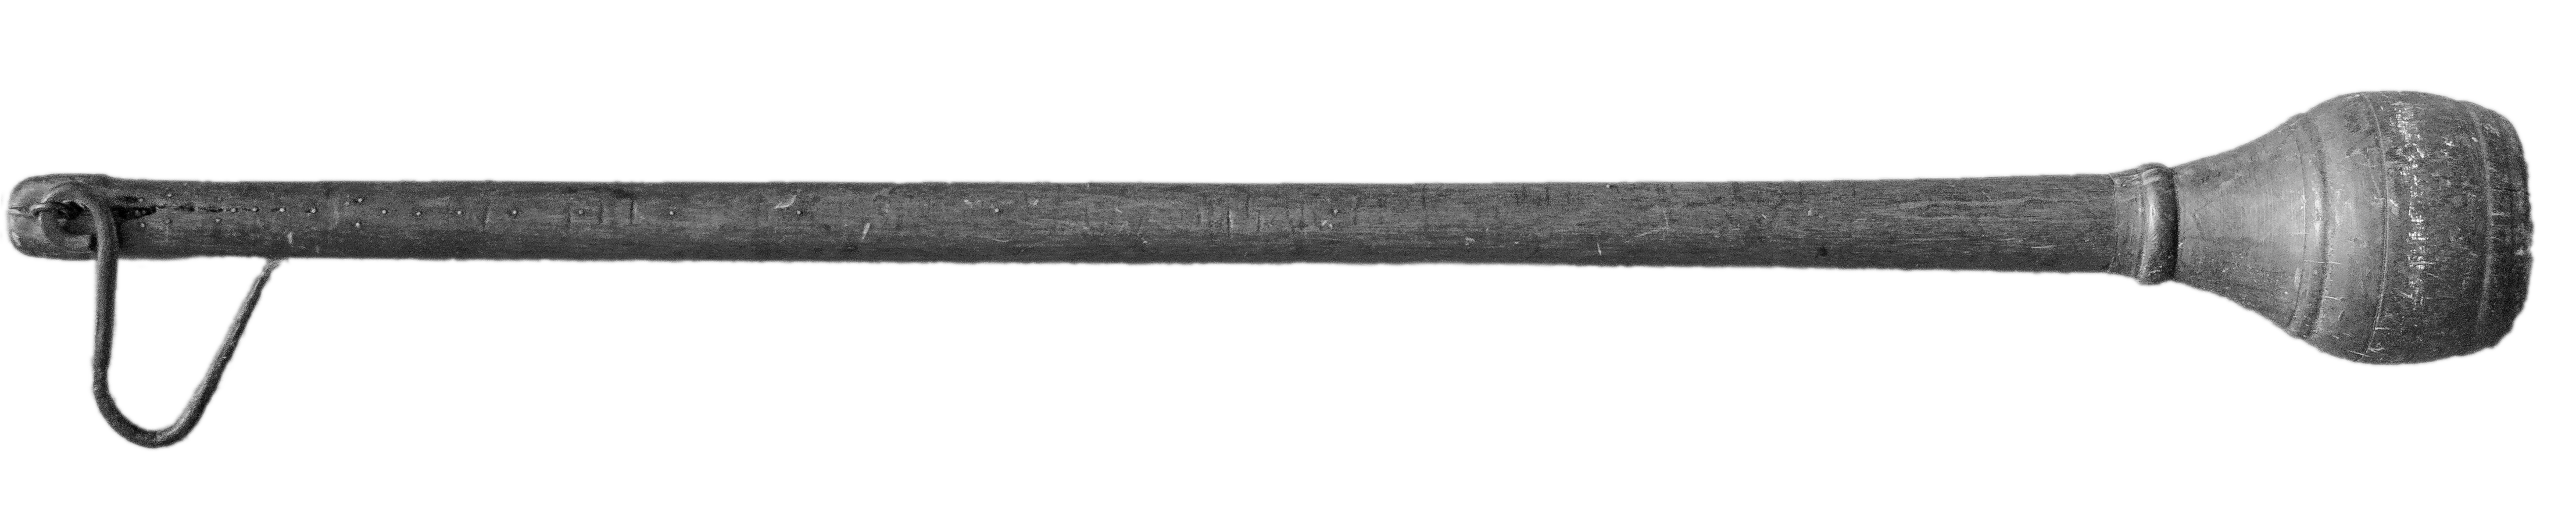
\includegraphics[width=12cm]{pics/puupuntari.png}
  \caption{A wooden \emph{besman} from 1818. The wooden bulb hides a lead weight}
  \label{fig:besman}
\end{figure}


\begin{table}
\begin{tabular}{lcccc|cl}
  & \emph{läst} & \emph{skeppund} & \emph{pund} & \emph{mark} & Metric &
  Symbol \\
  \hline
  \emph{läst}        & 1 & 12 & 240 & 4800 &  1560 kg & \sample{läst} \\
  \emph{skeppund}    &   & 1  & 20  &  400 &  130 kg &
  \sample{\abskeppund}, \sample{\abskeppundtwo} \\
  \emph{besmanspund}, \emph{pund} &   &    & 1   &  20 &  6.54 kg  &
  \sample{\abbesmanspund}, \sample{\abpund}, \sample{\abpundtwo} \\
  \emph{besmansmark}, \emph{mark} &   &    &     &  1 &   327 g & \sample{\abmark},
  \sample{\abmarc} \\
\end{tabular}
  \caption{Stockholm \emph{besman} weights of early 16th century}
  \label{tab:besman_weights}
\end{table}


A \emph{besman} (\emph{puntari} in Finnish) is a beam lever scale with
a fixed counterweight. In medieval times they were usually made from
wood with a lead weight in the end. When weighing things with them one
finds the balance point on the lever and reads the mark at that point.
Besmans are less precise than scales so it usually wasn't possible to
measure smaller units than half a \emph{mark} and the heavier the
measured thing was, the less precision was available for the results.


\begin{description}
\item [\sample{läst} \emph{Läst}, \emph{lästi}]
  \mbox{} \\
  A \emph{läst} was a large unit that was used to measure ship loads.
  Because of the cargo aspect, it was used as a weight measure only
  for heavy commodities such as metals. For other products a
  \emph{läst} was usually measured in barrels (\emph{tunna}).

  With metals a \emph{läst} was typically 12 \emph{skeppunds}, or
  around two metric tons depending on which particular \emph{skeppund}
  was used.

  The word \emph{läst} was usually not abbreviated in texts.
  \begin{center}
    \begin{tabular}{llll}
      {}läst  & \sample{\abkolmannes} & \ltxncmd{ablast} \\
    \end{tabular}
  \end{center}

\item [\sample{\abskeppund}, \sample{\abskeppundtwo} \emph{Skeppund},
  \emph{kippunta}, \emph{talentum navale}] \mbox{} \\
  The \emph{skeppund} was the largest Swedish weight unit (around
  130–180 kg). Beacause of the large size it is typically used only
  for metals and when describing large stockpiles of commodities such
  as salted fish. In Latin sources it was often written as
  \emph{talentum navale}.

  A \emph{skeppund} was usually divided into 20 \emph{punds}, but
  there are some 14th century references for having 24 \emph{pund}
  \emph{skeppunds}.

  \begin{center}
    \begin{tabular}{llll}
      {}skep[pund]  & \sample{\abskeppund} & \ltxncmd{abskeppund} \\
      {}[skeppund]  & \sample{\abskeppundtwo} & \ltxncmd{abskeppundtwo} \\
    \end{tabular}
  \end{center}


\item [\sample{\abbesmanspund}, \sample{\abpund}, \sample{\abpundtwo},
  \sample{\abpundthree}, \sample{\abpundfour} \emph{Besmanspund}, \emph{pund}, \emph{leiviskä}] \mbox{} \\
The \emph{besmanspund} (or shorter \emph{pund}) was the besman weight
equivalent of \emph{lispund} but in some regions the name
\emph{lispund} was used for both. In many areas, for example in
Stockholm, a \emph{lispund} was reckoned to be a \emph{besmanspund}
and two \emph{besmansmarks}.

In most areas \emph{besmanspund} was lighter than the proper
\emph{lispund}. For example, in Stockholm it was about 6.5 kg.
However, on the other end of the scales was the Porvoo \emph{pund}
that was about 13 kg for a while. The most common besman weight around
Northern Baltic was Tallinn \emph{lispund} that was used for trading
and taxation in many areas, for example, in most of Finland. Most
contemporary conversion tables state that the Tallinn \emph{lispund}
was equal to 25 Stockholm \emph{besmansmark}, but some use more exact
figure of $24\frac{27}{40}$ \emph{besmansmark}.

Confusingly many writers used the Latin abbreviation \emph{libra}
(\sample{\abbesmanspund}) for \emph{besmanspunds} even though it was
used also the much lighter \emph{skålpund}.

\begin{center}
  \begin{tabular}{llll}
    {}[libra]  & \sample{\abbesmanspund} & \ltxncmd{abbesmanspund} \\
    {}[pund]  & \sample{\abpund} & \ltxncmd{abpund} \\
    {}[p~ud]  & \sample{\abpundtwo} & \ltxncmd{abpundtwo} \\
    {}[~p]  & \sample{\abpundthree} & \ltxncmd{abpundthree} \\
    {}[~pp]  & \sample{\abpundfour} & \ltxncmd{abpundfour} \\
  \end{tabular}
\end{center}


\begin{table}
  \centering
  \begin{tabular}{lc}
    Year & Scale / Besman \\
    \hline 
    1490 &  $8/7$ \\
    1540 &  $22/20$ \\
    1557 &  $21/20$ \\
  \end{tabular}
  \caption{Weight ratios between Stockholm scale and besman on some years}
  \label{tab:stockholm_weight_ratio}
\end{table}


\begin{table}
  \centering
  \begin{tabular}{llll}
    Stockholm & 6.5 kg \\
    Tallinn \emph{lispund}  & 8.2 kg &  25 Stockholm \emph{besmansmark} \\
    Turku town \emph{leiviskä} & 9.8 kg & 30 Stockholm    \emph{besmansmark} \\
    Turku castle tax \emph{leiviskä} & 8.2 kg & Tallinn \emph{lispund} \\
    Hollola \emph{leiviskä} & 9.2 kg  & 28 Stockholm \emph{besmansmark} \\
    Pohjanmaa \emph{leiviskä} & 9.5 kg & 29 Stockholm    \emph{besmansmark} \\
    Porvoo \emph{leiviskä} & 13 kg & 2 Stockholm \emph{besmanspund}   \\
    Raasepori \emph{leiviskä} & 9.8 kg & 30 Stockholm    \emph{besmansmark} \\
    Satakunta \emph{leiviskä} & 9.8 kg & 30 Stockholm  \emph{besmansmark} \\
    Turku castle \emph{leiviskä} & 6.8 or 6.5 kg & Four marks lighter
    than tax \emph{leiviskä} \\
  \end{tabular}
  \caption{Some different besman weights. Conversion rations from
    various times of the 16th century, using contemporary rounding.
  }
  \label{tab:lispunds}
\end{table}



\item [\sample{\abmark}, \sample{\abmarc} \emph{Besmansmark},
  \emph{mark}, \emph{naula}] \mbox{} \\
  The basic unit for besman weights was \emph{besmansmark} that was
  usually called simply \emph{mark}. A \emph{besmansmark} was
  typically about 50\% heavier than the precious metal \emph{mark} or
  approximately 330 g, but the size range goes around 300–400g.

  The \emph{besmansamark} was written the same way as the precious
  metal \emph{mark}.
    \begin{center}
    \begin{tabular}{llll}
      {}[mark]  & \sample{\abmark} & \ltxncmd{abmark} \\
      {}[mark:] & \sample{\abmarc} & \ltxncmd{abmarc}    \\
      {}[mark::] & \sample{\abmk} & \ltxncmd{abmk}  \\
    \end{tabular}
  \end{center}
\end{description}



\subsection{Dry Volume}


Old Swedish weight measurement systems are simple compared with the
systems for measuring dry capacity by volume. The basic unit was
\emph{spann} in most parts of the whole realm, but its size and how it
divided and combined into other units varied greatly. 

Modern estimates on sizes of different units in different places at
different times vary greatly so the figures given in tables should be
taken with a large grain of salt. The figures are generally obtained
by using conversion ratios that occur in old texts (typically tax
accounts) from some known base. Sam Jansson gives the size of
Stockholm's \emph{spann} as 47 liters that he calculated from the size
of a surviving Lübeck \emph{schepel} (40.5 liters) measure from early
15th century and conversion rates Lübeck and Stockholm units given in a
letter written in 1405.\footnote{Number 16524 in \emph{Svenskt
    Diplomaratiums huvudkartor över medeltidsbreven} (SDHK).}

In the tables I've generally used Jansson's figures. For those that
I've calculated myself, I used Jansson's Stockholm \emph{spann} as the
fixed point. These results are different from many published values.
For example, the size of a Häme \emph{spann} is usually given as
"about 90 liters", but my computation has it at only 66 liters.
However, I am using a conversion rate that comes from over hundred
years later than Jansson's figures for Stockholm's unit, so it is
possible that something had changed in the mean time. The sizes of at
least Pohjanmaa and Viipuri \emph{spann} changed during the 16th
century. 

\begin{table}
\begin{tabular}{lccccc|cl}
  & \emph{pund} & \emph{tunna} & \emph{spann}  & \emph{fjärding} & \emph{fat} & Metric &  Symbol \\
  \hline
  \emph{pund}      & 1 &  $3 \frac{1}{5}$ & 8  & 32 & 160 & 376 l  &  \sample{\abpund}, \sample{\abpundthree}  \\
  \emph{tunna}     &   &  1 & $2 \frac{1}{2}$ & 10 & 50   & 117.5 l &  \sample{\abtunna}   \\
  \emph{spann}     &   &    & 1     & 4  & 20   & 47 l    &  \sample{\abspann}   \\
  \emph{fjärding}  &   &    &       & 1  &  5   & 11.75 l &  \sample{\abfjarding}   \\  
  \emph{fat}       &   &    &       &    &  1   &  2.35 l & \sample{fat} \\
  \emph{skäppa}    &   &    &  $\frac{5}{12}$ &    &      & 19.6 l  &  \sample{\abskappa}   \\
\end{tabular}
  \caption{Stockholm dry capacity units}
  \label{tab:stockholm_volume}
\end{table}


This section contains quite few tables for dry volume units from all
over Sweden, with a heavy emphasis on the Finnish side. The ratios
between units are probably mostly correct, but the modern equivalences
may well not be.

\begin{table}
\begin{tabular}{lcccc|cl}
  & \emph{pund} & \emph{spann}  & \emph{fjärding} & \emph{skåle} &  Metric &  Symbol \\
  \hline

  \emph{pund}      & 1 & 5 & 20 & 120 & 450 l & \sample{\abpund} \\
  \emph{spann}     &   & 1 & 4  & 24  & 90 l   & \sample{\abspann} \\
  \emph{fjärding}  &   &   & 1  &  6  & 22.5 l & \sample{\abfjarding} \\
  \emph{skåle}     &   &   &    &  1  & 3.l5 l & \sample{\abskole}  \\
\end{tabular}
  \caption{Närke dry capacity units}
  \label{tab:narke_volume}
\end{table}





\begin{description}









\item [\sample{fat} \emph{fat}] \mbox{} \\
  The \emph{fat} (bowl) was a Swedish measure that was used in the
  middle ages. Its size had a large variance, and it ranged from 20
  \emph{fat} in a Stockholm \emph{spann} (2.35 liters) to a fifth of a
  \emph{spann}. The Finnish crown accounts often used 'Stockholm
  \emph{kappa}' in unit conversions when they meant Stockholm
  \emph{fat}.
  \begin{center}
    \begin{tabular}{llll}
      {}fat  & \sample{\abfat} & \ltxncmd{abfat} \\
    \end{tabular}
  \end{center}

\item [\sample{\abfjarding}, \sample{\abfjardingtwo} \emph{fjärding},
  \emph{nelikko}, \emph{neljännes}, \emph{quartale modii}] \mbox{} \\
  A \emph{fjärding} was a fourth of a \emph{spann}. In Finland the
  unit was usually called \emph{nelikko} or \emph{neljännes} but some
  areas used different names for it. For example, \emph{vakka} was
  commonly used for $\frac{1}{4}$ \emph{spann} around Turku. 

  After the \emph{tunna} replaced \emph{pund} as the main large unit
  for dry capacity, both \emph{fjärding} and \emph{nelikko} switched
  to mean a quarter \emph{tunna} instead of a quarter \emph{spann}.
  But that didn't happen until mid-16th century.
  \begin{center}
    \begin{tabular}{llll}
      {}~ffi  & \sample{\abfjarding} & \ltxncmd{abfjarding} \\
      {}fjard~ug & \sample{\abfjardingtwo} & \ltxncmd{abfjardingtwo}    \\
    \end{tabular}
  \end{center}


\item [\sample{\abkappa}, \sample{\abkappatwo}, \emph{kappe}, \emph{kappa}] \mbox{} \\
  A \emph{kappa} was a Finnish unit that was used in large parts of
  the country as the smallest unit of dry volume and it still
  survives: it is used to measure potatoes in marketplaces. The
  \emph{kappa} was typically in the range of 3–5 liters in modern
  units and there were 16 to 24 of them in a \emph{spann}.

  The \emph{kappa} is one of the oldests units attested in Finland, it
  first occurs in a letter written in 1334. In the 16th century
  \emph{kappa} was written with either intial \emph{k} or \emph{c}.
  When the Finnish spelling got standardized in the early 17th
  century, the form \emph{cappa} took over and was used for about 150
  years until \emph{kappa} returned around the end of the 19th
  century.

  After the middle ages the name \emph{kappa} was taken to Swedish as
  a loan word \emph{kappe}.
  \begin{center}
    \begin{tabular}{llll}
      {}cap[per]  & \sample{\abkappa} & \ltxncmd{abkappa} \\
      {}kap[per] & \sample{\abkappatwo} & \ltxncmd{abkappatwo}    \\
    \end{tabular}
  \end{center}


\begin{table}
\begin{tabular}{lccc|cl}
  & \emph{pund} & \emph{spann}  & \emph{fjärding}  &  Metric &  Symbol \\
  \hline
  \emph{pund}      & 1 & 12 & 48 & 360 l & \sample{\abpund} \\
  \emph{spann}     &   & 1 & 4   & 30 l   & \sample{\abspann} \\
  \emph{fjärding}  &   &   & 1   & 7.5 l & \sample{\abfjarding} \\
\end{tabular}
  \caption{Hälsingaland dry capacity units}
  \label{tab:halsingaland_volume}
\end{table}
\begin{table}
  \begin{tabular}{lcccc|cl}
    & \emph{pund} & \emph{tön} & \emph{spann} & \emph{sättung} & Metric
    & Symbols\\
    \hline 
    \emph{pund}      & 1 & $1\frac{1}{3} $ &  8 & 48 & 380 l &
    \sample{\abpund}, \sample{\abpundthree} \\ 
    \emph{tön}       &   & 1 &  6 & 36 & 360 l & \sample{\abthyn} \\
    \emph{spann}     &   &   &  1 &  6 &  60 l & \sample{\abspann} \\
    \emph{sättung}   &   &   &    &  1 &  10 l & \sample{\absixth}\\
  \end{tabular}
  \caption{Uppland dry capacity units}
  \label{tab:uppland_volume}
\end{table}





\item [\sample{\abkarpio} \emph{karp}, \emph{karpio}] \mbox{} \\
  A \emph{karpio} was another specifically Finnish unit that occurs
  also in Swedish texts under the name \emph{karp}. It was a half of a
  \emph{spann} in size or approximately 30 liters.

  Some Latin texts written in Finland use \emph{modius} to mean a
  \emph{karpio} instead of a \emph{spann}.
  \begin{center}
    \begin{tabular}{llll}
      {}*k[per]  & \sample{\abkarpio} & \ltxncmd{abkarpio} \\
      {}k        & \sample{\abkarpiotwo} & \ltxncmd{abkarpiotwo} \\
      {}mo~d & \sample{\abmodius} & \ltxncmd{abmodius}    \\
    \end{tabular}
  \end{center}
  


\item [\sample{\abkolmannes} \sample{\abkylmitta} \emph{kolmannes},
  \emph{kylmitta}, \emph{oravainen}] \mbox{} \\
  The \emph{kolmannes}, \emph{kylmitta} and \emph{oravainen} were
  names for similar units that were used in Finland. As the name
  \emph{kolmannes} tells, they all were thirds of something. The names
  \emph{kolmannes} and \emph{oravainen} were used in Savo to denote a
  third of a \emph{karpio} so the size was somewhat over 10 liters. At
  Viipuri \emph{kolmannes} and \emph{kylmitta} were used for a third
  of a \emph{spann}, making them about 18 liters in size.
  \begin{center}
    \begin{tabular}{llll}
      {}kol~m  & \sample{\abkolmannes} & \ltxncmd{abkolmannes} \\
      {}kyl~m & \sample{\abkylmitta} & \ltxncmd{abkylmitta}    \\
    \end{tabular}
  \end{center}


\begin{table}
\begin{tabular}{lcccccc|cl}
  & \emph{lästi} & \emph{punta} & \emph{panni} & \emph{karpio} &
  \emph{nelikko} & \emph{vakka} & Metric &  Symbol \\
  \hline
  \emph{lästi}     & 1 & 12 & 60 & 120 & 240 & 1440 & 3.96 m$^2$ & \sample{\ablast} \\
  \emph{punta}     &   &  1 &  5 &  10 &  20 &  120 & 330 l & \sample{\abpund} \\
  \emph{panni}    &   &    &  1 &   2 &   4 &   24 & 66 l & \sample{\abspann}\\
  \emph{karpio}     &   &    &    &   1 &   2 &   12 & 33 l & \sample{\abkarpio}\\
  \emph{nelikko} &   &    &    &     &   1 &    6 & 16.5 l & \sample{\abfjarding} \\
  \emph{vakka}    &   &    &    &     &     &    1 & 2.75 l & \sample{\abvakka}\\
\end{tabular}
\caption{Hämeo dry capacity units. The size of \emph{spann} is computed
  from 1540 accounts of Häme castle that gives a conversion rate of 5 Häme
  \emph{spann} to 7 Stockholm \emph{spann}.}
  \label{tab:hame_volume}
\end{table}

\begin{table}
\begin{tabular}{lcccc|cl}
  & \emph{pund} & \emph{spann} & \emph{vakka} & \emph{kappa} & Metric &  Symbol \\
  \hline 
  \emph{punta}   & 1 &  6 &  24 & 120  & 432 l & \sample{\abpund} \\
  \emph{panni}  &   &  1 &   4 &  20 & 72 l  & \sample{\abspann} \\
  \emph{vakka/nelikko}  & &    &   1 &   5 & 18 l  &  \sample{\abvakka}, \sample{\abfjarding} \\
  \emph{kappa}  &   &    &     &   1  & 3.6 l & \sample{\abkappa} \\
\end{tabular}
\caption{Varsinais-Suomi dry capacity computed using the conversion
  rate of 30 Turku \emph{kappa} = 46 Stockholm \emph{fat}. }
  \label{tab:turku_volume}
\end{table}


\item [\sample{\ablast} \emph{läst}, \emph{lästi}] \mbox{} \\
  The \emph{läst} was the largest unit for volume measurements as it
  was also for weight measurements. The läst could be counted in two
  different ways:

  \begin{itemize}
  \item \emph{pundeläst}: a \emph{läst} containing a specific number
    of \emph{punds}, typically 12.
  \item \emph{tunnaläst}: a \emph{läst} containing a specific number
    of \emph{tunnas}, usually 12 or 18. 
  \end{itemize}

  As a \emph{pund} was usually much greater unit than \emph{tunna}, a
  \emph{pundeläst} could be well over 10 times greater in volume than
  a \emph{tunnaläst}.

  \begin{center}
    \begin{tabular}{llll}
      {}läst  & \sample{\abkolmannes} & \ltxncmd{ablast} \\
    \end{tabular}
  \end{center}


\item [\sample{\abskole} \emph{skåle}] \mbox{} \\
  The \emph{skåle} was the smallest unit of dry capacity measure in Närke
  and Västmanland. There 24 \emph{skåle} in a \emph{spann}. 
  \begin{center}
    \begin{tabular}{llll}
      {}skaale  & \sample{\abskole} & \ltxncmd{abskole} \\
    \end{tabular}
  \end{center}

\item [\sample{\abpund}, \sample{\abpundthree}
  \emph{pund}, \emph{punta}] \mbox{} \\
  In most parts of Sweden the principal large unit for dry volume was
  the \emph{pund}. The most typical \emph{pund} contained eight
  \emph{spann} but that too varied. Around \emph{Närke} and
  \emph{Häme} there were only five \emph{spann} in a pund, and in most
  parts of Finland there were six. The areas with smallest
  \emph{spanns} had 12 to a \emph{pund}. 

  The Stockholm \emph{pund} was about 380 liters in modern units. 
  \begin{center}
    \begin{tabular}{llll}
      {}[pund]  & \sample{\abpund} & \ltxncmd{pund} \\
      {}p~ud  & \sample{p~ud} & \ltxncmd{abpundtwo} \\
      {}~p & \sample{\abpundthree} & \ltxncmd{abpundthree} \\
      {}~pp & \sample{\abpundfour} & \ltxncmd{abpundfour} \\
    \end{tabular}
  \end{center}


\item [\sample{\abspann}, \sample{\abmodius}
  \emph{spann}, \emph{panni}, \emph{modius}] \mbox{} \\
  The size of the base unit \emph{spann} varied greatly. In
  Hälsingaland it was only 30 liters while Närke used \emph{spann} of
  over 90 liters. Perhaps the most common sizes were around 60 liters,
  but the capital Stockholm used only 47 liter ones.

  Latin texts often used the term \emph{modius} to denote the
  \emph{spann}, but \emph{modius} was used also for many different
  units in different parts.
    \begin{center}
    \begin{tabular}{llll}
      {}~sp  & \sample{\abspann} & \ltxncmd{abspann} \\
      {}mo~d & \sample{\abmodius} & \ltxncmd{abmodius} \\
    \end{tabular}
  \end{center}


\begin{table}
\begin{tabular}{lccccc|cl}
  & \emph{punta} & \emph{panni} & \emph{karpio} & \emph{kolmannes} & \emph{kappa} & Metric &  Symbol \\
  \hline
  \emph{punta}      & 1 &  6 & 12 & 36 & 108 & 396 l & \sample{\abpundthree}\\
  \emph{panni}     &   &  1 &  2 &  6 &  18 & 66 l & \sample{\abspann} \\
  \emph{karpio}    &   &    &  1 &  3 &   9 & 33 l & \sample{\abkarpio}\\
  \emph{kolmannes} &   &    &    &  1 &   3 & 11 l & \sample{\abkolmannes} \\
  \emph{kappa}     &   &    &    &    &   1 & 3.7 l & \sample{\abkappa}\\
\end{tabular}
\caption{Savo dry capacity units. Computed from equivalence where 1
  Savo \emph{kolmannes} = $4\frac{2}{3}$ Stockholm \emph{fat}.}
  \label{tab:savo_volume}
\end{table}



\item [\sample{\absoll} \emph{såll}, \emph{cribrum}] \mbox{} \\
  Västergotaland and Värmland used \emph{såll} as the the larger unit
  than \emph{skäppa} or \emph{spann}. Later the unit fell out of use
  and was replaced by \emph{tunna} that had the same size as
  \emph{såll} in those areas.
  \begin{center}
    \begin{tabular}{llll}
      {}saaldh & \sample{\absoll} & \ltxncmd{absoll} \\
    \end{tabular}
  \end{center}


\begin{table}
\begin{tabular}{lcccccc|lc}
  & \emph{punta} & \emph{panni} & \emph{karpio} & \emph{kylmitta} & \emph{vakka} & \emph{kappa} & Metric &  Symbol \\
  \hline
  \emph{punta}   & 1 &  6 & 12 &  18 & 108 & 138 & 324 l & \sample{\abpund} \\
  \emph{panni}   &   &  1 &  2 &  3  &  18 & 23 & 54 l & \sample{\abspann}\\
  \emph{karpio}  &   &    &  1 &  $1 \frac{1}{2}$ & 9 & & 27 l & \sample{\abkarpio} \\
  \emph{kylmitta} &  &    &    &  1  &   6 &    & 18 l & \sample{\abkylmitta} \\
  \emph{vakka}  &   &    &     &     &   1 &   & 3 l & \sample{\abvakka} \\
  \emph{kappa}  &   &    &     &     &     &    1   & 2.35 l & \sample{\abkappa} \\
\end{tabular}
\caption{Viipuri dry capacity. Computed from equivalence: Viipuri
  \emph{spann} = 23 Stockholm \emph{fat}. In the late  16th century
  the size of Viipuri \emph{spann} changed several times, ranging from
  23 \emph{fat} to 26.}
  \label{tab:viipuri_volume}
\end{table}




\begin{table}
\begin{tabular}{lcccc|cl}
  &  \emph{läst} & \emph{såll} & \emph{skäppa}  & \emph{fjärding} &  Metric &  Symbol \\
  \hline
  \emph{läst}      & 1 & 12 & 72 & 288 & 1.728 m$^3$ & \sample{läst} \\  
  \emph{såll/tunna}     &   &  1 & 6  & 24  & 144 l & \sample{\absoll}, \sample{\abtunna}  \\
  \emph{skäppa}    &   &    & 1  &  4  &  24 l & \sample{\abskappa}  \\
  \emph{fjärding}  &   &    &    &  1  &   6 l & \sample{\abfjarding} \\  
\end{tabular}
  \caption{Västergötaland dry capacity units}
  \label{tab:vastgotaland_volume}
\end{table}


\item [\sample{\abskappa}, \sample{\abmodius} \emph{skäppa}, \emph{modius}] \mbox{} \\
  In Västergötaland and Småland the base volume unit was not the
  \emph{spann} but the \emph{skäppa}. In these areas the Latin
  \emph{modius} usually ment the \emph{skäppa} instead of the
  \emph{spann}. In size the \emph{skäppa} was somewhat smaller than
  the \emph{spann} with its size ranging from 18 to 23 liters.

  The Stockholm \emph{skäppa} was unusual in that it was not
  fully integrated in the complete system of measurements. It was
  reckoned to be 5/12 \emph{spann} (aobut 19.6 liters) which meant
  that it did not divide any of the units exactly.
  \begin{center}
    \begin{tabular}{llll}
      {}skäppa & \sample{\abskappa} & \ltxncmd{abskappa} \\
      {}mo~d & \sample{\abmodius} & \ltxncmd{abmodius} \\
    \end{tabular}
  \end{center}

  \begin{table}
    \centering
    \begin{tabular}{lcccc|cl}
      &              \emph{Lästi} & \emph{Punta} & \emph{Panni} &
      \emph{Vakka} & Metric & Symbol \\
      \hline
      \emph{Lästi}  &  1  &  12  &  96  & 960 &     4 $m^3$ & \sample{\ablast}\\
      \emph{Punta}  &     &   1  &   8  &  80 &    336 l  &  \sample{\abpund}, \sample{\abpundthree}  \\
      \emph{Panni}  &     &      &   1  &  10 &     42 l  &       \sample{\abspann} \\
      \emph{Vakka}  &     &      &      &   1 &    4.2 l  & \sample{\abvakka} \\
    \end{tabular}
    \caption{Pohjanmaa dry capacity units. Computed from ratio 1
      \emph{panni} = 18 Stockholm \emph{fat}}
    \label{tab:pohjanmaa_volume}
  \end{table}



\item [\sample{\absattung} \emph{sättung} ] \mbox{} \\
  Dalsland and Uppland areas divided their \emph{spanns} into sixths
  \emph{sättung} instead of fourths (\emph{fjärding}). The size of a
  \emph{sättung} was approximately 10 liters in modern units. 
  \begin{center}
    \begin{tabular}{llll}
      {}s* & \sample{\absattung} & \ltxncmd{absattung} \\
    \end{tabular}
  \end{center}

\item [\sample{\abtunna}, \sample{\abtunnor}] \emph{tunna}, \emph{tynnyri} \mbox{} \\
  The \emph{tunna} (barrel) was a rare unit in that it had a separate
  abbreviation for the plural \emph{tunnor}:
  \begin{center}
    \begin{tabular}{cc}
      \sample{\abtunna} & \sample{\abtunnor} \\
      tunna (s) & tunnor (pl) \\
    \end{tabular}
  \end{center}

  In the oldest times it was primarily a measure for wet goods but
  slowly over the time it became used also for dry capacity. Mentions
  of dry \emph{tunnas} are quite rare before the 15th century, then
  they became more common until by mid-16th century it is in very
  common use for grain.

  With dry capacity a \emph{tunna} ranged from 1.5 \emph{spann} to 4
  \emph{spann}. In modern units its size was typically in the range
  110–150 l. The size of \emph{tunna} tended to increase over time and
  a late 16th century \emph{tunna} is typically larger than a 15th
  century one. The \emph{tunna} of the Stockholm castle was 2.5
  Stockholm \emph{spanns} or about 120 liters.

  \begin{center}
    \begin{tabular}{llll}
      {}[tunna] & \sample{\abtunna} & \ltxncmd{abtunna} \\
      {}[tunna] & \sample{\abtunnor} & \ltxncmd{abtunnor} \\
    \end{tabular}
  \end{center}


\item [\sample{\abthyn} \emph{tön} ] \mbox{} \\
  The \emph{tön} or \emph{thyn} was a large unit that was used instead
  of \emph{pund} in early times in Uppland and neighbouring areas. It
  was later replaced by \emph{pund}, but the last mentions of
  \emph{tön} go to the late 16th century.

  There were six \emph{spann} in a \emph{tön} so it was slightly
  smaller than a \emph{pund}. 
  \begin{center}
    \begin{tabular}{llll}
      {}þyn & \sample{\abthyn} & \ltxncmd{abthyn} \\
    \end{tabular}
  \end{center}


\item [\sample{\abvakka} \emph{vakka}] \mbox{} \\
  A \emph{vakka} was a Finnish unit that had very large variance in
  size. In some areas (for example, Häme and Viipuri) it was the
  smallest unit of dry volume at about three liters in size. However,
  in other areas it contained some multiples of \emph{kappas},
  typically four or five. For example, at Turku a \emph{vakka} was
  used as a synonym for \emph{nelikko} and it contained five
  \emph{kappas}.
  \begin{center}
    \begin{tabular}{llll}
      {}vacka & \sample{\abvakka} & \ltxncmd{abvakka} \\
    \end{tabular}
  \end{center}
\end{description}


\subsubsection{Hay and straw} 






 \begin{table}
   \centering
   \begin{tabular}{lcccc|cl}
        & \emph{Kesä} & \emph{Talvi- } \\
        & \emph{kuorma} & \emph{kuorma} & \emph{Dragu} &  \emph{Parmas} & Metric & Symbol \\
     \hline
     \emph{Talvikuorma} & 1 & 2 & 4 & 8 & 4.4 m$^3$ &  \sample{lass} \\
     \emph{Kesäkuorma}  &   & 1 & 2 & 4 & 2.2 m$^3$ &  \sample{\absommarlass} \\
     \emph{Dragu}       &   &   &   & 1 & 1.1 m$^3$ &  \sample{\abdragu} \\
     \emph{Parmas}      &   &  &   &  1 & 0.55 m$^3$ &  \sample{\abparmas} \\
   \end{tabular}
   \caption{Larger Häme straw measurements. Metric sizes are very
     rough approximations computed by assuming a \emph{parmas} of 120
     cm long straws with a 2.4 meter circumference. }
   \label{tab_hay}
 \end{table}

Measuring the volume of hay and straw stores was usually done using
special units\footnote{However, there are occasional mentions of
  \emph{punds} of hay in account books.} The units and the ratios
between them here are taken mostly from Finnish sources. 

Translating the hay units to modern terms is almost impossible as they
were vague already at the time and the way they were used varied a lot
even in a small geographical area. 

\begin{description}

\item [\sample{lass} \emph{lass}, \emph{kuorma}] \mbox{} \\
  The \emph{lass} is the unit of hay and straw volume that occurs most
  often in medieval and early modern accounts. Its size is very
  difficult to determine exactly but generally it was as much hay that
  could be transported with one cart or sleigh. In many areas two
  different \emph{lasses} were used at the same time: the larger
  winter \emph{lass} (\emph{vinterlass}, \emph{talvikuorma}) and the
  smaller summer \emph{lass} (\emph{sommarlass}, \emph{kesäkuorma}).
  Some sources also use the term tax \emph{lass}, which probably meant
  the larger \emph{vinterlass}

  A winter \emph{lass} might be about 3–5 m$^3$ in size. In Finland a
  summer \emph{lass} was often half of the size of a winter
  \emph{lass}.

  \begin{center}
    \begin{tabular}{llll}
      {}lass & \sample{\ablass} & \ltxncmd{ablass} \\
      {}vin[ter]lass & \sample{\abvinterlass} & \ltxncmd{abvinterlass} \\
      {}so~marlass & \sample{\absommarlass} & \ltxncmd{absommarlass} \\
    \end{tabular}
  \end{center}



\item [\sample{\abparmas}, \emph{parmas}] \mbox{} \\
  The \emph{parmas} was a Finnish united defined to be the amount of
  hay or straw that can be tied for transport using a cord of a given
  length. For example, at Viipuri it was a cord of 4 \emph{famn} (a
  bit over 7 m) that is tied crosswise, while at Sääksmäki the cord
  was 8 \emph{aln} (about 4 m) but it is not mentioned if the rope was
  crosswise or not.

  In Finland a \emph{talvikuorma} usually contained 8 \emph{parmas}
  but some areas used 12 \emph{parmas} per \emph{kuorma}. 
  \begin{center}
    \begin{tabular}{llll}
      {}[par]mas & \sample{\abparmas} & \ltxncmd{abparmas} \\
    \end{tabular}
  \end{center}


\item [\sample{faangh} \emph{fångh}, \emph{ruko}] \mbox{} \\
  The \emph{fångh} contained as much hay that a person could carry
  without tying the bundle up. A common computational ratio was that
  there would be four \emph{ruko} in a \emph{parmas}.
  \begin{center}
    \begin{tabular}{llll}
      {}faangh & \sample{\abfangh} & \ltxncmd{abfangh} \\
    \end{tabular}
  \end{center}

\item [\sample{kärffue} \emph{kärve}, \emph{kupo}] \mbox{} \\
  The \emph{kärve} was reckoned to be as much hay that a person could
  carry under their arm. A common computation in Finland was that
  there was four \emph{kupo} in a \emph{ruko}.
  \begin{center}
    \begin{tabular}{llll}
      {}kärffue & \sample{\abkarve} & \ltxncmd{abkarve} \\
    \end{tabular}
  \end{center}


\item [\sample{dragu} \emph{dragu}] \mbox{} \\
  The origins of the unit \emph{dragu} are obscure. The word is
  originally Swedish but it is attested only in Finnish accounts
  before the 17th century.
  
  The \emph{dragu} had a large variation in size. For example, the
  accounts of the Korsholma royal manor have it to be roughly the size
  of common \emph{parmas} but around Viipuri a \emph{dragu} was a
  synonym for \emph{kesäkuorma}, or about four times the amount. 

  Some parts of Finland used two different \emph{dragu}: winter and
  summer where a winter \emph{dragu} was twice the size of the summer
  \emph{dragu}.

  \begin{center}
    \begin{tabular}{llll}
      {}dragu & \sample{\abdragu} & \ltxncmd{abdragu} \\
      {}v~iterdragu & \sample{\abvinterdragu} & \ltxncmd{abvinterdragu} \\
      {}so~mardragu & \sample{\absommardragu} & \ltxncmd{absommardragu} \\
    \end{tabular}
  \end{center}
  

\item [\sample{\abaam} \emph{åm}, \emph{aami} ] \mbox{} \\
  Several areas in Finland used the \emph{aami} to measure hay in
  addition of its use as a wet capacity measurement. It was generally
  used as a synonym to \emph{parmas}. 
  \begin{center}
    \begin{tabular}{llll}
      {}aam & \sample{\abaam} & \ltxncmd{abaam} \\
    \end{tabular}
  \end{center}



\end{description}



\subsection{Wet capacity}

The units that were used to measure wet capacity were simpler than the
dry capacity ones. Their sizes varied on different parts of the
country, but the units themselves tended to be the same.


\begin{table}
  \centering
  \begin{tabular}{lcccccc|cl}
    & \emph{Läst} & \emph{Tunna} & \emph{Fjärding} & \emph{Ämbar} & \emph{Kanna} &
    \emph{Stop} & Metric & Symbol \\
    \hline
    \emph{Läst}     & 1 & 12 & 48 & 144 & 576 & 1152 & 1410 l & \sample{\ablast} \\
    \emph{Tunna}    &   & 1  &  4 &  8  & 48  & 96   & 117.5 l & \sample{\abtunna}\\
    \emph{Fjärding} &   &    &  1 &  2  & 12  & 24   &  29.4 l & \sample{\abfjarding} \\
    \emph{Ämbar}    &   &    &    &  1  & 6   & 12   &  14.7 l & \sample{\abambar} \\
    \emph{Kanna}    &   &    &    &     & 1   &  2   &  2.4 l & \sample{\abkanna} \\
    \emph{Stop}     &   &    &    &     &     &  1   &  1.2 l & \sample{\abstop} \\
  \end{tabular}
  \caption{Wet capacity units based on the Rostock barrel}
  \label{tab_large_wet_a}
\end{table}



\begin{description}
\item [\sample{\abstop} \emph{stop}, \emph{tuoppi} ]\mbox{} \\
  During the high middle ages the base unit for measuring wet goods in
  the Baltic areas was the \emph{stop}. The name translates to a
  \emph{tankard}. The size of a \emph{stop} varied in different areas,
  in modern units it varied from somewhat under liter to over. The
  most common size of \emph{stop} in the later middle ages was
  probably 1.2 liters that was one 1/96 of the Rostock \emph{barrel}.
  In the 17th century it got standardized to 1.3 liters. 
  \begin{center}
    \begin{tabular}{llll}
      {}stope & \sample{\abstop} & \ltxncmd{abstop} \\
    \end{tabular}
  \end{center}



\item [\sample{\abquarter}, \emph{kvarter}, \emph{kortteli}] \mbox{} \\
  Later sources divide a \emph{stop} into four \emph{kvarters} but it
  is not certain if the unit was used already during the middle ages.
  \begin{center}
    \begin{tabular}{llll}
      {}q~t & \sample{\abquarter} & \ltxncmd{abquarter} \\
    \end{tabular}
  \end{center}


\item [\sample{\abkanna}, \sample{\abkannatwo} \emph{kanna}, \emph{kannu} ]\mbox{} \\
  During the 15th century the \emph{kanna} ("jug") replaced the
  \emph{stop} as the base unit. There were two \emph{stops} in a
  \emph{kanna}, meaning that it ranged from a bit under two liters to
  almost three liters. The \emph{kanna} that corresponded to the size
  of the Rostock barrel was 2.45 liters in size. The later
  standardization fixed \emph{kanna} to 2.6 liters.
  \begin{center}
    \begin{tabular}{llll}
      {}[kanna] & \sample{\abkanna} & \ltxncmd{abkanna} \\
      {}ka~na & \sample{\abkannatwo} & \ltxncmd{abkannatwo} \\
    \end{tabular}
  \end{center}

\item [\sample{\abtunna}, \sample{\abtunnor} \emph{tunna}, \emph{tynnyri}] \mbox{} \\
  The primary large wet capacity measure was a \emph{tunna} (barrel)
  from the earliest times. The most common barrel size in use around
  the Baltic sea was the Rostock barrel of 117.5 liters, but others
  were also in use. 

  In the middle ages a typical \emph{tunna} contained 48 \emph{kanna},
  but during the 16th century it became common to use larger barrels
  and there are mentions of 50 or 52 \emph{kanna} \emph{tunnas}.
  \begin{center}
    \begin{tabular}{llll}
      {}[tunna] & \sample{\abtunna} & \ltxncmd{abtunna} \\
      {}[tunna] & \sample{\abtunnor} & \ltxncmd{abtunnor} \\
    \end{tabular}
  \end{center}
  

\item [\sample{\abfjarding}, \sample{\abfjardingtwo} \emph{fjärding}, \emph{nelikko}, \emph{neljännes}] \mbox{} \\
  A \emph{fjärding} was the fourth of a \emph{tunna} for wet capacity
  measurements so its size was about 30 liters. Note that while both
  \emph{fjärding} and \emph{kvarter} mean a \emph{fourth}, they are
  units of very different sizes. 
  \begin{center}
    \begin{tabular}{llll}
      {}~ffi & \sample{\abfjarding} & \ltxncmd{abfjarding} \\
      {}fiärd~ug & \sample{\abfjardingtwo} & \ltxncmd{abfjardingtwo} \\
    \end{tabular}
  \end{center}


\item [\sample{\abambar}, \sample{\abotting} \emph{ämbar},
  \emph{åtting}, \emph{ämpäri}  ] \mbox{} \\
  A half of a \emph{fjärding} was either \emph{åtting} (en eighth) or
  \emph{ämbar} (a bucket) in different parts of the country. Its size
  was approximately 15 liters. 
  \begin{center}
    \begin{tabular}{llll}
      {}ämbar & \sample{\abambar} & \ltxncmd{ämbar} \\
      {}attu~g & \sample{\abotting} & \ltxncmd{abotting} \\
    \end{tabular}
  \end{center}


\begin{table}
  \centering
  \begin{tabular}{lccc|cl}
    &  \emph{Båt} & \emph{Åm} & \emph{Kanna} & Metric &
    Symbol \\
    \hline
    \emph{Båt}   & 1 & 3 & 180 & 440 l & \sample{\abbaat} \\
    \emph{Åm}, \emph{fat}    &   & 1 &  60 & 147 l & \sample{\abaam}, \sample{fat}  \\
    \emph{Kanna} &   &   &   1 & 2.4 l & \sample{\abkanna} \\
  \end{tabular}
  \caption{Wet capacity units for blubber and wine}
  \label{tab_large_wet_b}
\end{table}


\item [\sample{\abaam}, \sample{fat} \emph{åm}, \emph{aami}] \mbox{} \\
  The \emph{åm} was used to measure seal blubber. Later it became also
  a measure for wine. In that role it was a synonym for \emph{fat}.
  The an \emph{åm} was reckoned to be equal to 60 \emph{kanna} (about
  150 liters) in volume  and for blubber  20 \emph{lispund} in weight.
  \begin{center}
    \begin{tabular}{llll}
      {}aam & \sample{\abaam} & \ltxncmd{abaam} \\
      {}fat & \sample{\abfat} & \ltxncmd{abfat} \\
    \end{tabular}
  \end{center}



\item [\sample{\abbaat} \emph{båt}] \mbox{} \\
  Wine and seal blubber trade used \emph{båt} to measure large
  quantities. A \emph{båt} contained three \emph{åm}, or approximately
  450 liters in volume. For blubber it was 60 \emph{lispund} in
  weight.
  \begin{center}
    \begin{tabular}{llll}
      {}baat & \sample{\abbaat} & \ltxncmd{abbaat} \\
    \end{tabular}
  \end{center}

\end{description}


\subsection{Length measures}

The units of length were mostly same with same rations in the whole
Sweden, but their exact sizes were different in different areas. It is
possible to establish a few of them exactly as they were marked on the
walls or doors of stone churches. For example, the door of Vadsbo
church had marks for the \emph{halvaln} of about 32 cm, which gives
the length of Västergötland \emph{aln} to be 64 cm. Three churches
(Stånga, Havdhem and Hemse) all have markings for the Gotland
\emph{aln}. They are not exactly equal, 55.4 cm at Stånga and Hemse
while 55.1 cm at Hemse, but they are close enough that we can reckon
that the Gotland \emph{aln} was a bit over 55 cm.

\begin{table}
  \centering
  \begin{tabular}{ll}
    Area  & Modern \\
    \hline
    Gotland  & 55.4 cm \\
    Götlunda & 62.8 cm \\
    Lund &  55.7 cm \\
    Stockholm "new"& 52.5 cm \\
    Stockholm "old "& 55.5 cm \\
    Vadstena & 53.9 cm \\
    Västergötland & 64 cm \\
    Öland & 47 cm \\
    Östergotland & 59.4 cm \\
  \end{tabular}
  \caption{\emph{Aln} lengths that are known with some certainty.}
  \label{tab_aln_lengths}
\end{table}


\begin{table}
  \centering
  \begin{tabular}{lcccccc|ll}
    & \emph{Stång} & \emph{Famn} & \emph{Aln} & \emph{Fot} &
    \emph{Quarter} & \emph{Tum} & Metric & Symbol \\
    Stång & 1 & 2 & 6 & 12 & 24 & 144 & 3.15 m & \sample{\abstang} \\
    Famn  &   & 1 & 3 &  6 & 12 &  72 & 1.58 m & \sample{\abfamn} \\  
    Aln   &   &   & 1 &  2 &  4 &  24 &  52.5 cm & \sample{aln} \\
    Fot   &   &   &   &  1 &  2 &  12 &  26.3 cm & \sample{fot}\\
    Quarter & &   &   &    &  1 &   6 &  13.1 cm & \sample{\abquarter}\\
    Tum   &   &   &   &    &    &   1 &   2.2 cm & \sample{tum} \\
  \end{tabular}
  \caption{Stockholm length measures }
  \label{tab_length}
\end{table}


\begin{description}
\item [\sample{aln} \emph{aln}, \emph{kyynärä}] \mbox{} \\
  The basic length unit was \emph{aln} (\emph{kyynärä}) that
  corresponds to cubit. Its length varied between 47–65 cm in
  different areas. The Stockholm \emph{aln} was one of the shortest
  with its 52.5 cm length.
  \begin{center}
    \begin{tabular}{llll}
      {}aln & \sample{\abaln} & \ltxncmd{abaln} \\
    \end{tabular}
  \end{center}


\item [\sample{\abquarter} \emph{kvarter}, \emph{kortteli}] \mbox{}
  \\
  The principal division of an \emph{aln} was to divide it into four
  quarters of 12–16 cm. The Stockholm \emph{kvarter} was 13.1 cm long.
  \begin{center}
    \begin{tabular}{llll}
      {}q~t & \sample{\abquarter} & \ltxncmd{abquarter} \\
    \end{tabular}
  \end{center}

  
\item [\sample{fot} \emph{fot}, \emph{jalka}] \mbox {} \\
  The foot (\emph{fot}, \emph{jalka}) was also used in Sweden, but was
  secondary compared with \emph{aln} and \emph{quarter} and some
  places used a \emph{halvaln} instead. There were two \emph{quarters}
  in a \emph{fot} and two \emph{fot} in an \emph{aln}. 
  \begin{center}
    \begin{tabular}{llll}
      {}fot & \sample{\abfot} & \ltxncmd{abfot} \\
      {}halvaln & \sample{\abhalvaln} & \ltxncmd{abhalvaln} \\
    \end{tabular}
  \end{center}


\item [\sample{tum} \emph{tum}, \emph{tuuma}] \mbox{} \\
  The \emph{tum} was the equivalent of inch and there were six
  \emph{tum} in a \emph{quarter} and 24 \emph{tum} in an \emph{aln}.
  The Stockholm \emph{tum} was 2.2 cm long.
  \begin{center}
    \begin{tabular}{llll}
      {}tum & \sample{\abtum} & \ltxncmd{abtum} \\
    \end{tabular}
  \end{center}


\item [\sample{ffa~pn} \emph{famn}, \emph{syli}] \mbox{} \\
  The \emph{famn} was the equivalent of a fathom. In most parts of
  Sweden there were three \emph{aln} per \emph{famn} but in Norrland
  each \emph{famn} contained 3 1/2 \emph{aln}.
  \begin{center}
    \begin{tabular}{llll}
      {}ffa~pn & \sample{\abfamn} & \ltxncmd{abfamn} \\
    \end{tabular}
  \end{center}

\item [\sample{\abstang} \emph{stång}, \emph{tanko}] \mbox{} \\
  The \emph{stång} corresponded to a rod. It was typically six
  \emph{aln} long, but in parts of Östergötland and Småland also five
  \emph{aln} \emph{stång} was used and there are occasional records
  for eight \emph{aln} lengths.
  \begin{center}
    \begin{tabular}{llll}
      {}[stång] & \sample{\abstang} & \ltxncmd{abstang} \\
    \end{tabular}
  \end{center}

\item [\sample{mil}, \sample{rast} \emph{mil}, \emph{rast}, \emph{peninkulma}] \mbox{} \\
  The \emph{mil} was a length measure with a vague length that varied
  a lot in different parts of Sweden. The old name for the unit was
  \emph{rast} but that got superseded by \emph{mil} during the middle
  ages. The \emph{mil} in Finland corresponded to about 6 modern
  kilometers while the \emph{mil} in Dalarland was almost three times
  that length with its 15 km distance. Before the country was surveyed
  it was not possible to measure long distances exactly so all
  measurements that are given in \emph{mils} are approximations. Later
  \emph{mil} was standardized to 18000 \emph{aln} but that didn't
  happen until the 17th century.
  \begin{center}
    \begin{tabular}{llll}
      {}mil & \sample{\abmil} & \ltxncmd{abmil} \\
      {}rast & \sample{\abrast} & \ltxncmd{abrast} \\
    \end{tabular}
  \end{center}

\item [\sample{vika}, \sample{vecka} \emph{vecka}, \emph{sjömil}]
  \mbox{} \\
  The \emph{vika} or \emph{vecka} was the marine equivalent of
  \emph{mil} (hence, \emph{sjömil} or sea \emph{mil}). It too was
  vaguely defined, but it seems to have been approximately 7.5 km in
  modern terms.
  \begin{center}
    \begin{tabular}{llll}
      {}vika & \sample{\abvika} & \ltxncmd{abvika} \\
      {}vecka & \sample{\abvecka} & \ltxncmd{abvecka} \\
    \end{tabular}
  \end{center}

\end{description}


\begin{table}
  \centering
  \begin{tabular}{ll}
    Unit & Modern  \\
    \hline
    Västgötaland \emph{mil} & ~13 km  \\
    Småland \emph{mil} & ~7.5 km \\
    Dalarland \emph{mil} & ~15 km \\
    Finland \emph{mil} & ~6 km \\
    \emph{Vecka} (\emph{sjömil}) & ~7.5 km \\
  \end{tabular}
  \caption{Long distance measurements}
  \label{tab_long_distance}
\end{table}



\subsection{Area}

During the medieval times there were two main reasons for measuring
land: taxation and economical. The crown wanted to assess how much
taxes a farm could or should pay, and a landowner (especially a noble
one with many estates) wanted to know how much a farm could produce.
Determining the exact land area in the modern sense was not necessary
for either purpose.

The capacity to pay taxes was not completely determined by its size
but also the land quality and opportunities for non-farming income
such as fishing affected it. For this reason the medieval units for
area are extremely vague and using them was highly subjective. There
were some rough guidelines but they were not used as binding rules.
For example, in the 16th century Hälsingaland a \emph{spannland} was
reckoned to be a square of field with eight \emph{stång} sides or
about 830 m$^2$, but this assumed "good land".

In general, only fields and meadows were measured and the units can be
roughly divided into three classes:

\begin{itemize}
\item units directly tied to the amount of taxes that should be paid
  (e.g. \emph{marksland}, \emph{öresland}). 
\item units describing how much grain is sown in the field
  (\emph{tunnland}, \emph{spannland})
\item units tied to units of length (e.g. \emph{stång}, \emph{aln})
\end{itemize}

Some units, like \emph{pundsland} were used in two senses: they were
both units for measuring seed grain and also abstract units for
taxation.

\subsubsection{Tax units}

In the areas that used taxation based on land area, the basic
principle was that each village had some amount of taxes assigned to
it, and that tax was then allocated to individual farms by counting
what proportion of the fields it owned.

For example, suppose that there was a village that had been assessed
to be two \emph{rök} in size. The crown assigned the taxed so that
each \emph{rök} had to pay a specific amount of taxes, so in this
example the village would need to pay two tax units.


\definecolor{lgray}{HTML}{A09B9B}
\definecolor{dgray}{HTML}{6A6767}

\begin{figure}
  \centering
  \begin{tabular}{ll}
    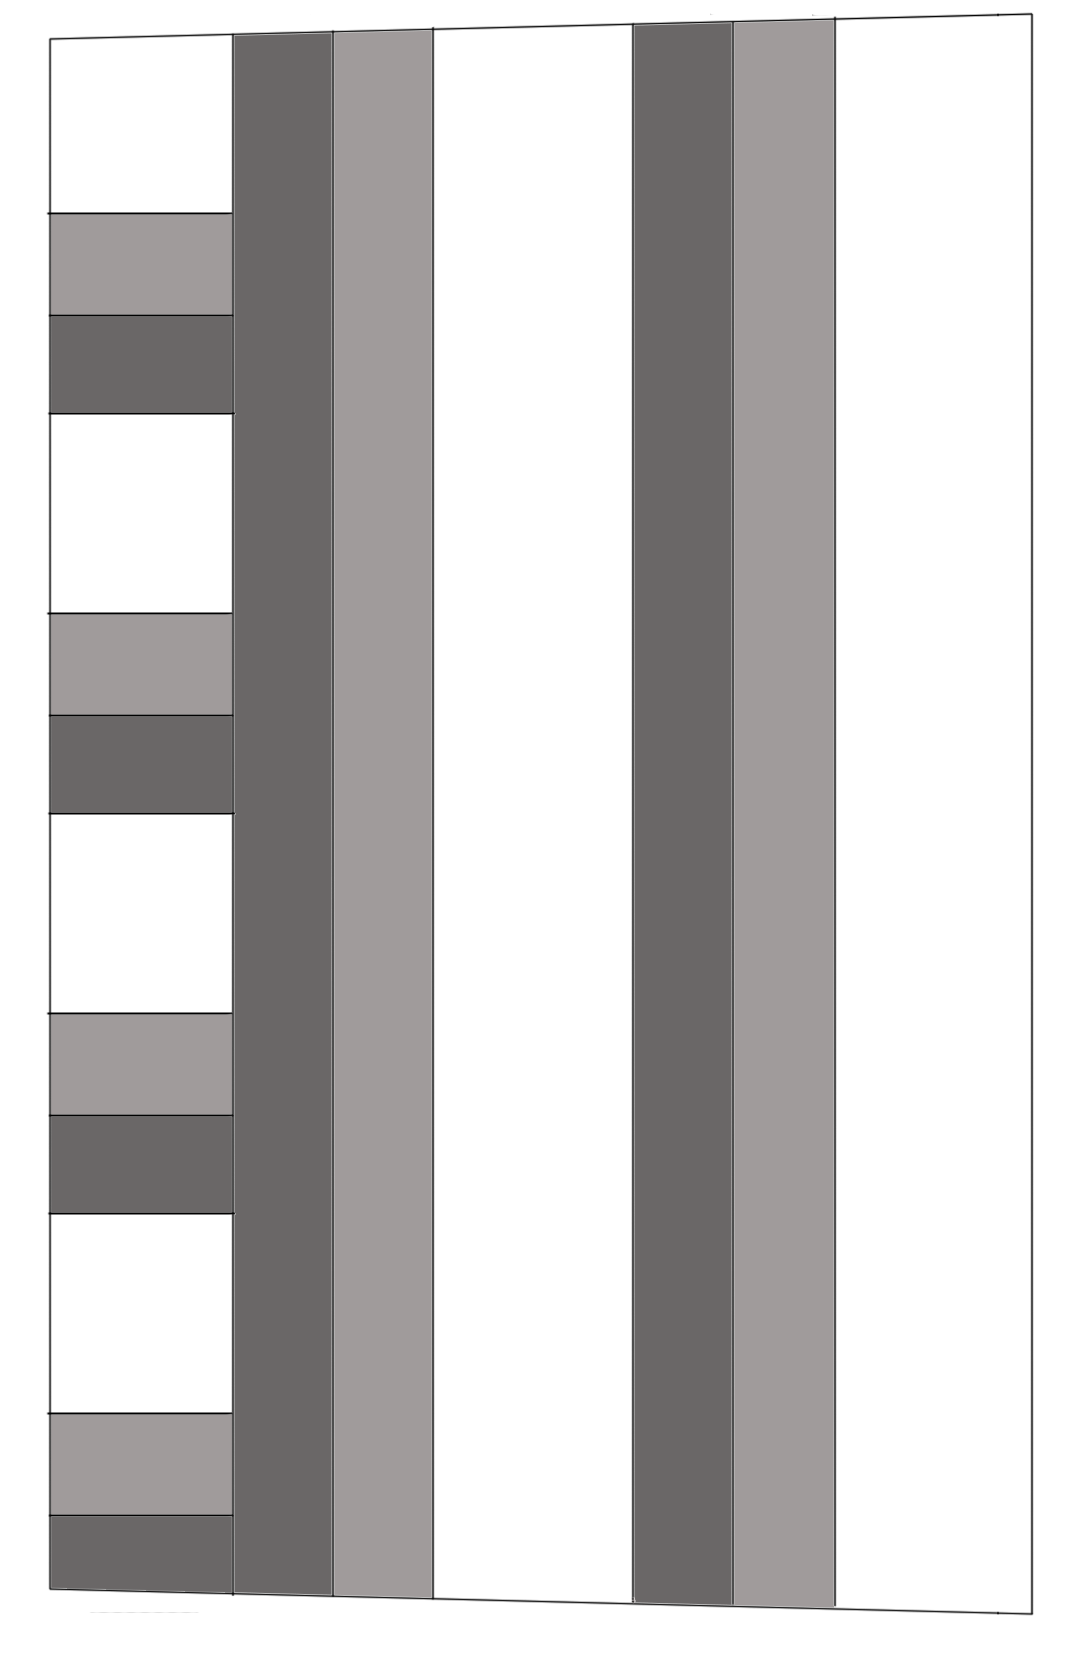
\includegraphics[width=4cm]{pics/fields.png} &
    \raise3cm\hbox{\smash{\begin{minipage}{6cm}
      \begin{tabular}{llll}
        A & 2 \emph{stång} & 3 \emph{öre} &  \fcolorbox{black}{white}{\phantom{TEST}}      \\
        B & 1 \emph{stång} & $1\frac{1}{2}$ \emph{öre}  &\fcolorbox{black}{lgray}{\phantom{TEST}}
        \\
        C & 1 \emph{stång} & $1\frac{1}{2}$ \emph{öre} & \fcolorbox{black}{dgray}{\phantom{TEST}} \\
      \end{tabular}
    \end{minipage}}}
  \end{tabular}
  \caption{The \emph{stång} division of a field in a village of 6 \emph{öresland} and 4 \emph{stång}.} 
  \label{fig:stong}
\end{figure}

The \emph{rök} would then be divided into smaller parts. In Upper
Satakunta each \emph{rök} had 12 \emph{öresland}. Each village was
allocated some number of \emph{öres} out of the \emph{rök}. Each farm
of the village was allocated a number of \emph{stångs}. The communal
fields of the village were divided into thin strips and allocated to
the farms in proportion to the \emph{stångs} of the farms. The farm
also had to pay taxes in proportion to its \emph{stång} count. This is
illustrated in figure \ref{fig:stong}. Typically each \emph{stång}
corresponded to 1–2 \emph{öres}.

\begin{table}
  \centering
  \begin{tabular}{lll}
    Area & Unit & Divides into  \\
    \hline
    Varsinais-Suomi & \emph{rök}, \emph{savu} & 32 \emph{öresland} \\
    Ala-Satakunta   & \emph{rök}, \emph{savu} & 12 \emph{öresland} \\
    Ylä-Satakunta   & \emph{krok}, \emph{koukku} & 12 \emph{öresland} \\
    Häme            & \emph{krok}, \emph{koukku} & 12 \emph{öresland}
    \\
    Länsi-Uusimaa   & \emph{skattemark}, \emph{veromarkka} & 18 \emph{aln} \\
    Itä-Uusimaa     & \emph{full skatte}, \emph{täysvero} & 18 \emph{aln} \\
    Kymenkartano    & \emph{full skatte}, \emph{täysvero} & 18 \emph{aln} \\
    Viipurin lääni  & \emph{full skatte}, \emph{täysvero} & \\
    Savo            & \emph{skatteskin}, \emph{veronahka} &  \\
    Pohjanmaa       & \emph{pundsland}, \emph{punnanala} & 10 \emph{spannland} \\
    Åland           & \emph{marksland} \\
                    & \emph{rök} \\
                    & \emph{full skatte} \\
  \end{tabular}
  \caption{Land-area based taxation units in Finland according to \cite{seppala09}}
  \label{tab_taxation_units}
\end{table}



\begin{description}
\item [\sample{\abmarksland}, \emph{marksland}, \emph{markanmaa}] \mbox{} \\
  \emph{Marksland} was perhaps the oldest taxation unit in Sweden for
  agricultural areas. Originally it denoted an area that was supposed
  to pay one \emph{mark} in taxes, but over time it became a
  computational unit. In Finnish side it was used only at Åland.
  \begin{center}
    \begin{tabular}{llll}
      {}[mark]aland & \sample{\abmarksland} & \ltxncmd{abmarksland} \\
      {}[mark::]al~ad & \sample{\abmarkslandtwo} & \ltxncmd{abmarkslandtwo} \\
    \end{tabular}
  \end{center}

  
\item [\sample{\aboresland}, \emph{öresland}, \emph{äyrinmaa}] \mbox{} \\
  Originally \emph{aboresland} was the amount of land suposed to pay
  an \emph{öre} in taxes. Later it was used as a computational
  division for other units, such as \emph{rök}, \emph{krok},
  \emph{skattemark}, and \emph{marksland}. 
  \begin{center}
    \begin{tabular}{llll}
      {}[ore]sl~ad & \sample{\aboresland} & \ltxncmd{aboresland} \\
    \end{tabular}
  \end{center}

\item [\sample{\abortugsland}, \emph{örtugsland}, \emph{aurtuanmaa}] \mbox{} \\
  An \emph{ortugsland} was a further subdivision of an \emph{öresland}. 
  \begin{center}
    \begin{tabular}{llll}
      {}[ortug]al~ad & \sample{\abortugsland} & \ltxncmd{abortugsland} \\
    \end{tabular}
  \end{center}

\item [\sample{\abpenningsland}, \emph{penningsland},
  \emph{penninmaa}]
  \mbox{} \\
  The smallest subdivision of a \emph{marksland} was
  \emph{penningsland}. It was already so small that there are not that
  many mentions of it in sources.
  \begin{center}
    \begin{tabular}{llll}
      {}pe~nal~ad & \sample{\abpenningsland} & \ltxncmd{abpenningsland} \\
    \end{tabular}
  \end{center}



\item [\sample{rök}, \emph{rök}, \emph{savu}] \mbox{} \\
  A \emph{rök} (\emph{smoke}) originally meant a single inhabited farm
  but it evolved into a general land measure for taxation. It kept the
  original meaning in most of Finland for the whole middle ages, but
  got the general meaning in Åland and Varsinais-Suomi.


\item [\sample{krok}, \emph{krok}, \emph{aura}] \mbox{} \\
  A \emph{krok} was also a specific unit that evolved into general
  land measure. It means \emph{a plough} and it is not certain whether
  it originally meant a single physical plough or the area that could
  be plowed with one team.


\item [\sample{skatheskin}, \emph{skatteskin}, \emph{veronahka}, \emph{oravainen}] \mbox{} \\
  A \emph{skatteskin} (\emph{tax skin}) was a taxation unit for areas
  without strong agriculture. Originally it denoted an area that was
  responsible for paying a set amount of fur skins as taxes, but as
  agriculture improved it became another general land area measure. A
  \emph{skatteskin} was also called \emph{oravainen} (\emph{little
    squirrel}) in Finnish, because the tax was usually assessed in
  winter squirrel skins.


\item [\sample{\abskattemark} \emph{skattemark},
  \emph{veromarkka},] \mbox{} \\
  The \emph{skattemark} was a unit that was used in two different
  senses. In some areas it was used like \emph{marksland} but it was
  divided into \emph{alns} instead of \emph{öreslands}. In Pohjanmaa
  where agriculture was poorly developed it was a property assessment:
  for each \emph{skattemark} of property there were in an area, the
  inhabitants had to collectively pay one silver mark of taxes.
  \begin{center}
    \begin{tabular}{llll}
      {}skathe[mark] & \sample{\abskattemark} & \ltxncmd{abskattemark} \\
    \end{tabular}
  \end{center}




\item [\sample{full skathe}, \emph{full skatte}, \emph{täysvero}] \mbox{} \\
  The \emph{full skatte} was a similar unit as \emph{markland} but it
  was introduced later and to different parts of the country. In areas
  with established agriculture it was divided into \emph{stångs} and
  \emph{alns}, while in Savo it was divided into halves, quarters, and
  eighths.

  \begin{table}
    \centering
    \begin{tabular}{lcccc|l}
                  & \emph{bol} & \emph{halvbol} & \emph{fjärding} & \emph{åtting} & Symbol \\
                  \hline
      \emph{bol}  &     1      &      2     &      4          &     8         & \sample{\abbol} \\
      \emph{halvbol}  &        &      1     &      2          &     4         & \sample{\abhalvbol} \\
      \emph{fjärding} &        &            &      1          &     2         & \sample{\abfjarding} \\
      \emph{åtting} &          &            &                 &     1         & \sample{\abotting} \\
    \end{tabular}
    \caption{The \emph{bol} division of land}
    \label{tab:bol}
  \end{table}

\item [\sample{halffskatte}, \emph{halv skatte}, \emph{puolivero}]
  \mbox{} \\
  The \emph{halv skatte} was a half of a \emph{full skatte}. 

\item [\sample{\abbol}, \emph{bol}] \mbox{} \\
  Like a \emph{rök}, a \emph{bol} originally meant one inhabited farm
  but it later became a general land measure. As a measure it was
  first divided into halves and quarters, but later it grew bigger and
  contained 20 \emph{skattemark}. In Finland \emph{bol} was used only
  in areas where the population was Swedish-speaking.

  \begin{center}
    \begin{tabular}{llll}
      {}booll & \sample{\abbol} & \ltxncmd{abbol} \\
    \end{tabular}
  \end{center}


\item [\sample{\abhalvbol}, \emph{halvbol} ]\mbox{} \\
  A half of a bol was a \emph{halvbol}. 
  \begin{center}
    \begin{tabular}{llll}
      {}halffbooll & \sample{\abhalvbol} & \ltxncmd{abhalvbol} \\
    \end{tabular}
  \end{center}

\item [\sample{\abfjarding}, \sample{\abfjardingtwo}, \emph{fjärding}] \mbox{} \\
  During the middle ages a \emph{fjärding} was a fourth of a
  \emph{bol} or a \emph{full skatte}.
  \begin{center}
    \begin{tabular}{llll}
      {}~ffi  & \sample{\abfjarding} & \ltxncmd{abfjarding} \\
      {}fjard~ug & \sample{\abfjardingtwo} & \ltxncmd{abfjardingtwo}    \\
    \end{tabular}
  \end{center}

\item [\sample{\abotting}, \emph{otting}] \mbox{} \\
  An \emph{otting} was a eighth of a \emph{bol} or \emph{full skatte}.
  \begin{center}
    \begin{tabular}{llll}
      {}attu~g & \sample{\abotting} & \ltxncmd{abotting} \\
    \end{tabular}
  \end{center}
  

\end{description}



\subsection{Seed grain based units}

Measuring the size of a field by the amount of seed grain that was
sown to it was a common practice. However, the values were approximate
because the amount depended on the grain. For example, rye was sown in
a sparser pattern than barley and a farmer would use 30–50\% more
barley seeds than rye seeds on the same field. 

The most common crop rotation schema in Finland for normal fields was
that a half of farms fields were left fallow each year so a farmer
with 20 \emph{spannland} of land would sow 10 \emph{spanns} each year.


\begin{description}
\item [\sample{\abspannland} \emph{spannland},
  \emph{panninala}] \mbox{} \\
  A \emph{spannland} corresponded to the size of a field that was sown
  with a \emph{spann} of grain.
  \begin{center}
    \begin{tabular}{llll}
      {}~spl~ad & \sample{\abspannland} & \ltxncmd{abspannland} \\
    \end{tabular}
  \end{center}

\item [\sample{\abpundland} \emph{pundland},
  \emph{punnanala}] \mbox {} \\
  A \emph{pundland} corresponded to the size of a field that was sown
  with a \emph{pund} of grain.
  \begin{center}
    \begin{tabular}{llll}
      {}[pund]al~ad & \sample{\abpundland} & \ltxncmd{abpundland} \\
      {}p~udal~ad & \sample{\abpundlandtwo} & \ltxncmd{abpundlandtwo} \\
    \end{tabular}
  \end{center}

\item [\sample{\abtunnland} \emph{tunnland},
  \emph{tynnyrinala} ] \mbox{} \\
  The \emph{tunnland} corresponded to the size of a field that was
  sown with a \emph{tunna} of grain. The unit came to use when the
  \emph{tunna} was introduced as a dry measure so it was rare before
  the 16th century. 


\item [\sample{thynia}, \emph{thynia}] \mbox{} \\
  The unit \emph{thynia} occurs in some 14th century Swedish
  documents. It denoted the amount of land that could be sown with a
  \emph{thyn} of grain.

\end{description}


\subsection{Length based units} 

\begin{description}
\item [\sample{\abstang} \emph{stång}, \emph{tanko}] \mbox{} \\
  When \emph{stång} was used as a unit of area, it measured the width
  of a strip of field. It was also used as a computational unit of
  taxation as a measure of the general size of a farm without being
  tied to the actual area of the fields. As a computational unit there
  were usually 3 or 12–18 \emph{stång} in a taxation unit in Finland.
  \begin{center}
    \begin{tabular}{llll}
      {}[stång] & \sample{\abstang} & \ltxncmd{abstang} \\
    \end{tabular}
  \end{center}

\item [\sample{aln} \emph{aln}, \emph{kyynärä}] \mbox{} \\
  The \emph{aln} was used as an area measure in the same way as
  \emph{stång}. It was both a real measurement of strip width and a
  computational unit for taxation. 
  \begin{center}
    \begin{tabular}{llll}
      {}aln & \sample{\abaln} & \ltxncmd{abaln} \\
    \end{tabular}
  \end{center}
\end{description}




\subsection{Counting units}


\begin{table}
  \centering
  \begin{tabular}{llll}
    Name & Amount & Symbol & Usage \\
    \hline
    \emph{ask} & 1 & \sample{ask} & butter, honey \\
    \emph{boge} & 1 & \sample{boge} & men \\
    \emph{bok} & 24 & \sample{bok} & sheets of paper \\
    \emph{centener} & 12 & \sample{sintenre} & windowpanes \\
    \emph{dussin} & 12 & \sample{dussin} & merchandise \\
    \emph{gång}  & 4 & \sample{gaang} & horseshoes \\
    \emph{göpen} & inexact & \sample{göpen} & small things held in a hand \\
    \emph{hundra} & 100 & \sample{hundra} & anything \\
    \emph{kast}  &  4 & \sample{kast} & things held in hands (two in each) \\
    \emph{knippa} & various & \sample{knippa} & things bound together \\
    \emph{krok} & 1 & \sample{krok} & taxation unit (literal meaning \emph{plough}) \\
    \emph{par}   & 2 & \sample{par} & anything \\
    \emph{mantal} & various & \sample{mantal} & men \\
    \emph{näbbe} & 1 & \sample{nebbe} & adults \\
    \emph{näveful} & inexact & \sample{näuefull} & small things held in a hand \\
    \emph{rök} & 1 & \sample{rök} & farms (for taxation) \\
    \emph{skock} & 60 & \sample{skock} & merchandise \\
    \emph{släpp} & 2–10 & \sample{släpp} & dogs \\
    \emph{storhundra} & 120 & \sample{storhundra} & anything \\
    \emph{stycke} & 1 & \sample{\abstycke} & anything \\
    \emph{tolft} & 12 & \sample{tolft} & lumber \\
    \emph{tiogh} & 10 or 20 & \sample{tiogh} & eggs, planks \\
    \emph{däcker} & 10 & \sample{\abdacker} & furs, skins, sheets of parchment \\
    \emph{timber} & 40 & \sample{\abtimmer} & furs \\
  \end{tabular}
  \caption{Names for quantitites}
  \label{tab_quantities}
\end{table}


Some goods had separate units that were used for counting them. 

\begin{description}

\item [\sample{ask} \emph{ask}, \emph{aski}] \mbox{} \\
  An \emph{ask} was a small box made from wood or birch bark that was
  used when buying or selling small amounts of butter, honey, or
  similar substances. 

\item [\sample{boge}, \sample{b} \emph{boge}, \emph{jousi}] \mbox{} \\
  The \emph{boge} (a bow) was used to count men who were old enough to
  take part in hunting and it was perhaps the oldest unit of taxation
  in Finland. It is probable that it was originally used in a literal
  sense and every man who could draw a full-strength bow was counted.
  Later it was expanded to mean every men over a set age, often 14 or
  15.


\item [\sample{sintener} \emph{centener} ] \mbox{} \\
  The name \emph{centener} comes from Latin meaning 100, but for some
  obscure reason it was adopted to mean a group of 12 windowpanes in
  Sweden when glass windows started to be used. 

\item [\sample{dussin} \emph{dussin}, \emph{tusina}] \mbox{} \\
  A \emph{dussin} (a dozen) as a counting term (12) came to Sweden from
  Germany and it was quite rare during the middle ages and did not
  gain widspread use until the early modern times. It was usually used
  when buying or selling individual goods.

\item [\sample{gaang} \emph{gång}, \emph{kerta}] \mbox{} \\
  Horseshoes were counted in \emph{gångs}. A \emph{gång} had four
  shoes, enough to shoe one horse.

\item [\sample{hundra} \emph{hundra}] \mbox{} \\
  A \emph{hundra} means literally 'a hundred' and it was used as a
  unit meaning 100. This was also called \emph{lilla hundret}, meaning
  'a small hundred'.
  
\item [\sample{kast} \emph{kast}] \mbox{} \\
  A \emph{kast} was a unit that was used to count small things that
  could be carried in hand such as coins and nails. It usually denoted
  four items (two in both hands) but there were some exceptions. For
  example, in Jämntland a \emph{kast} of nails was 5 nails: three in
  one hand and two in another. 

\item [\sample{knippo} \emph{knippa}, \emph{nippu} ] \mbox{} \\
  A \emph{knippa} is a bundle where many things have been tied
  together somehow. How many things there were in a \emph{knippa}
  depended on what was being counted. For example, a \emph{knippa} of
  brooms was 10 pieces, and a \emph{knippa} of shingles was 100.

\item [\sample{mantal}, \emph{mantal}, \emph{manttaali} ] \mbox{} \\
  Under the old \emph{mantal} system a number of men were grouped
  together and they were collectively responsible for some obligation.
  For example, equipping a ship for the fleet. The number of men in a
  \emph{mantal} depended on area and the nature of obligation. In the
  16th century a new \emph{mantal} count was introduced that acted as
  an area measurement for taxation.

\item [\sample{nebbe}, \emph{näbbe}, \emph{nokka}] \mbox{} \\
  A \emph{näbbe} (\emph{beak}) was a person who was considered adult
  for the purpose of certain taxes. In some areas all adults were
  included in the \emph{näbbe} count, in other areas service folk were
  excluded.

\item [\sample{näuefull}, \sample{göpen} \emph{näveful},\emph{göpen}, \emph{koura} ] \mbox{} \\
  The \emph{näveful} was used when handling small things. It contained
  as much material that could be held in one closed hand. For example,
  in Finland it was common that a person who helped shearing sheep
  would receive as a salary a set number of \emph{koura} of wool.

\item [\sample{par} \emph{par}, \emph{pari} ] \mbox{} \\
  A \emph{par} is two of something. It was usually used to count
  things that come in pairs. 

\item [\sample{skock} \emph{skock}, \emph{parvi}] \mbox{} \\
  Like a \emph{dussin}, a \emph{skock} was a unit that was imported
  from Germany in late middle ages. It denoted 60 pieces and it too
  was mostly used for merchandise.

\item [\sample{släpp} \emph{släpp}, \emph{ajue}] \mbox{} \\
  A \emph{släpp} is a team of hunting dogs. You needed at least two
  dogs to have a \emph{släpp} but there might be several. 

\item [\sample{storhundra} \emph{storhundra} ] \mbox{} \\
  A \emph{storhundra} translates literally to "a big hundred" and it
  meant 120 pieces.

\item [\sample{stycke}, \sample{\abstycke} \emph{stycke},
  \emph{kappale}] \mbox{} \\
  A \emph{stycke} simply means a piece. It was used in account books
  as a unit in cases where there was no special unit to use.
  \begin{center}
    \begin{tabular}{llll}
      {}s~t & \sample{\abstycke} & \ltxncmd{abstycke} \\
    \end{tabular}
  \end{center}

\item [\sample{\abtimmer}, \sample{\abtimber} \emph{timmer}, \emph{timber}, \emph{kiihtelys}] \mbox{} \\
  In Finland furs were divided into two basic classes by their value:
  \emph{harmaanahka} (\emph{greyskin}) and \emph{valkonahka}
  (\emph{whiteskin}). The cheaper greyskins, most imortant of whom was
  the squirrel, were counted using a 40 piece \emph{kiihtelys} as the
  basic unit. In Swedish texts this is usually written either as
  \emph{timber} or \emph{timmer}. However, Swedish texts written in
  Finland often use \emph{timber} also when counting whiteskins, and
  then it means 10 of them.
  \begin{center}
    \begin{tabular}{llll}
      {}ti~m & \sample{\abtimmer} & \ltxncmd{abtimmer} \\
      {}[timber] & \sample{\abtimber} & \ltxncmd{abtimber} \\
    \end{tabular}
  \end{center}


\item [\sample{\abdacker} \emph{däcker}, \emph{tikkuri}] \mbox{} \\
  The more valuable whiteskins (such as winter ermine and black fox)
  were counted using a 10 piece \emph{tikkuri} as the unit in Finland.
  The word is a loan word from Swedish \emph{däcker} and it was used
  for also large skins and sheets of parchment. As mentioned above,
  Swedish texts written in Finland often use \emph{timber} for
  \emph{tikkuri} instead of \emph{däcker} when speaking about
  whiteskins.

\item [\sample{tiogh} \emph{tiogh}, \emph{tiu}] \mbox{} \\
  Originally a \emph{tiogh} computed in units of 10 and it was
  primarily used of planks. By the mid 16th century its meaning had
  changed to 20 pieces and it was most commonly used of eggs.

\item [\sample{tolft} \emph{tolft}, \emph{toltti} ] \mbox{} \\
  A \emph{tolft} (\emph{toltti} in Finnish) meant 12 pieces and it was
  most often used of lumber: beams and planks.

\end{description}

\subsubsection{Counting fish} 


There were particularly many different words for counting different
kinds of fish. Large amounts of fish were usually counted in barrels,
but for small amounts individual counts were used. 

\begin{table}
  \centering
  \begin{tabular}{llll}
    Name & Amount & Symbol & Usage \\
    \hline
    \emph{bast}  & 24 & \sample{bast} & eels and lampreys \\
    \emph{klove} & 100–240 & \sample{kloffue} & dried fish \\
    \emph{kärve} & 12–16 & \sample{kärue} & salmon \\
    \emph{rynkie} & 300 & \sample{rynkie} & whitefish \\
    \emph{snesa} & 20 & \sample{snes} & eels \\
    \emph{spide} & 24 & \sample{spidh} & fish \\
    \emph{stig} & 20 & \sample{stig} & fish \\
    \emph{stock} & 30 & \sample{stig} & fish \\
    \emph{val}   & 80 & \sample{val} & herring \\
    \emph{vårda} & 10 & \sample{vaardh}  & dried fish \\
  \end{tabular}
  \caption{Units for counting fish}
  \label{tab_fish}
\end{table}

\begin{description}
  
\item [\sample{bast} \emph{bast}] \mbox{} \\
  The \emph{bast} was used to count eels and lampreys and there were 24
  fish per \emph{bast}. 

\item [\sample{kloffue} \emph{klove}, \emph{pihti} ] \mbox{} \\
  The \emph{klove} was perhaps the most important unit for counting
  fish. It was used exclusively of dried fish and its size varied in
  different areas ranging from 100 to 240. It seems that in Stockholm
  there were 200 fish in a \emph{klove}. 

  In Finland \emph{klove} was called \emph{pihti} and it was used also
  for counting sheets of birch bark. When counting small fish like
  vendance a \emph{pihti} may have had up to 1000 fish.

\item [\sample{kärffue} \emph{kärve}] \mbox{} \\
  A \emph{kärve} was either 12 or 16 salmons.

\item [\sample{rynkie} \emph{rynkie} ] \mbox{} \\
  The \emph{rynkie} was a unit that was used in Satakunta to count
  whitefish. A \emph{rynkie} had 300 fish.

\item [\sample{snesa} \emph{snesa} ] \mbox{} \\
  The \emph{snesa} was another unit for counting eels. There were 20
  eels in a \emph{snesa}. 

\item [\sample{spidh} \emph{spide}] \mbox{} \\
  The \emph{spide} was used in Gotland to count all kinds of fish.
  There were 24 fish in a \emph{spide}. 

\item [\sample{stig} \emph{stig}] \mbox{} \\
  The \emph{stig} was also used to count all kinds of fish. There were
  20 fish in a \emph{stig}. 


\item [\sample{stock} \emph{stock}, \emph{joukko}] \mbox{} \\
  A \emph{stock} was a group of 30 fish. 

\item [\sample{val} \emph{val}, \emph{vaali}] \mbox{} \\
  The \emph{val} was a unit of counting herrings. Each \emph{val}
  had 80 herrings. 

\item [\sample{vaardh} \emph{vårda}, \emph{nippu}] \mbox{} \\
  A \emph{vårda} was a unit for dried fish (most often cods). A
  \emph{vårda} usually had 10 or 12 fish. A \emph{vårda} of lampreys
  typically had one more than other fish because one of them was used
  to tie the others.
  
\end{description}

%\fi

\section{LaTeX Command Reference }\label{reference}

\subsection{General commands}
\begin{description}
\item [\ltxncmd{abcursivefamily}] \mbox{} \\
  Switch to \Aboensis{} with the current size and set text color. This
  also makes \emph{~} and \emph{_} be normal letters.

\item [\ltxcmd{aboensis}{text}] \mbox{} \\
  Sets \package{text} in Aboensis with set text color. 

\item [\ltxncmd{abtildes}] \mbox{} \\
  Change \emph{~} and \emph{_} to normal letters. 

\end{description}

\subsection{Color handling}


\begin{description}

\item [\ltxcmd{abtext}{text}] \mbox{} \\
  Set \package{text} using the text color. 

\item[\ltxcmd{abrubric}{text}] \mbox{} \\
  Set \package{text} using the primary rubrics color. 
  

\item [\ltxcmd{abotherrubric}{text}] \mbox{} \\
  Set \package{text} using the secondary rubrics color. 
  
\item[\ltxncmd{abtorubric}] \mbox{} \\
  Change the color to the primary rubrics color. 

\item[\ltxncmd{abtootherrubric}] \mbox{} \\
  Change the color to the secondary rubrics color. 
  
\item [\ltxcmd{absettextcolor}{color}] \mbox{} \\
  Set the text color to \package{color}.
    
\item[\ltxcmd{absetrubriccolor}{color}] \mbox{} \\
  Set the primary rubric color to \package{color}.
  
\item[\ltxcmd{absetotherrubriccolor}{color}] \mbox{} \\
  Set the secondary rubric color to \package{color}. 
  
\item [\ltxcmd{absetcolormixpercentage}{percentage}] \mbox{} \\
  Set the primary rubrics color mix percentage to
  \package{percentage}.
  
\item [\ltxcmd{absetothercolormixpercentage}{percentage}]\mbox{} \\
  Set the secondary rubrics color mix percentage to
  \package{percentage}.

\item [\ltxncmd{abrubricred}]\mbox{}  \\
  Set the primary rubrics color to red (default). 

\item [\ltxncmd{abrubricgreen}]\mbox{}  \\
  Set the primary rubrics color to green. 


\item [\ltxncmd{abrubricblue}]\mbox{}  \\
  Set the primary rubrics color to blue. 

\item [\ltxncmd{abotherrubricred}]\mbox{}  \\
  Set the secondary rubrics color to red. 

\item [\ltxncmd{abotherrubricgreen}]\mbox{} \\
  Set the secondary rubrics color to green (default). 

\item [\ltxncmd{abotherrubricblue}]\mbox{} \\
  Set the secondary rubrics color to blue.

\end{description}

\subsection{Capitals and initials}


\begin{description}

\item [\ltxcmd{abcapital}{letter}] \mbox{} \\
  Add a two-colored capital letter with the primary rubrics color for
  highlighting. 

\item [\ltxcmd{abcapitalother}{letter}] \mbox{} \\
  Add a two-colored capital letter with the secondary rubrics color for
  highlighting.
  
\item [\ltxcmd{abinitial}{letter}] \mbox{} \\
  Add a Lombardic initial letter in the primary rubrics color. 

\item [\ltxcmd{abinitialother}{letter}] \mbox{} \\
  Add a Lombardic initial letter in the secondary rubrics color. 

\item [\ltxcmd{abinitialtwo}{letter}] \mbox{} \\
  Add a two-colored Lombardic inititial letter where main color is the
  primary rubrics color and the other color is the secondary rubrics
  color. 

\item [\ltxcmd{abinitialothertwo}{letter}] \mbox{} \\
  Add a two-colored Lombardic inititial letter where main color is the
  secondary rubrics color and the other color is the primary rubrics
  color.

\item [\ltxcmdfour{abinitwpos}{letter}{scale}{xpos}{ypos}] \mbox{} \\
  Add a Lombardic initial letter that is scaled by \feature{scale} and
  moved by \feature{xpos} and \feature{ypos}. The letter is in the
  primary rubrics color. 

\item [\ltxcmdfour{abinitowpos}{letter}{scale}{xpos}{ypos}] \mbox{} \\
  Add a Lombardic initial letter that is scaled by \feature{scale} and
  moved by \feature{xpos} and \feature{ypos}. The letter is in the
  secondary rubrics color. 

\item [\ltxcmdfour{abinittwowpos}{letter}{scale}{xpos}{ypos}] \mbox{}   \\
  Add a two-colored Lombardic initial scaled by \feature{scale} and
  moved by \feature{xpos} and \feature{ypos}. The main color is the
  primary rubrics color and the other color is the secondary rubrics
  color. 

\item [\ltxcmdfour{abinitotwowpos}{letter}{scale}{xpos}{ypos}] \mbox{}  \\
  Add a two-colored Lombardic initial scaled by \feature{scale} and
  moved by \feature{xpos} and \feature{ypos}. The main color is the
  secondary rubrics color and the other color is the primary rubrics
  color.

\item [\ltxcmd{abcursiveinitial}{letter}] \mbox{} \\
  Add a cursive initial \feature{letter} using the text color. 

\item [\ltxcmdfour{abcursiveinitialwithpos}{letter}{scale}{xpos}{ypos}] \mbox{} \\
  Add a cursive initial letter scaled by \feature{scale} and moved by
  \feature{xpos} and \feature{ypos}. 


\item [\ltxcmd{abstartchapter}{letter}{line}{line}] \mbox{} \\
  Add a two-line chapter start Lombardic initial and fhe first two
  lines of text. The initial is in the primary rubrics color.

\item [\ltxcmd{abstartchapterother}{letter}{line}{line}] \mbox{} \\
  Add a two-line chapter start Lombardic initial and fhe first two
  lines of text. The initial is in the secondary rubrics color.

\item [\ltxcmd{abstartchaptertwo}{letter}{line}{line}] \mbox{} \\
  Add a two-line chapter start with a two-colored Lombardic initial
  where main color is the primary rubrics color and the other is the
  secondary rubrics color. 


\item [\ltxcmd{abstartchapterothertwo}{letter}{line}{line}] \mbox{} \\
  Add a two-line chapter start with a two-colored Lombardic initial
  where main color is the secondary rubrics color and the other is the
  primary rubrics color. 

\item [\ltxcmd{abstartchapterwithpos}{letter}{scale}{xpos}{ypos}{line}{line}] \mbox{} \\
  Add a two-line chapter start with a scaled and positioned Lombardic
  initial in the primary rubrics color. 

\item [\ltxcmd{abstartchapterotherwithpos}{letter}{scale}{xpos}{ypos}{line}{line}]
  \mbox{} \\
  Add a two-line chapter start with a scaled and positioned Lombardic
  initial in the secondary rubrics color. 

\item [\ltxcmd{abstartchaptertwowithpos}{letter}{scale}{xpos}{ypos}{line}{line}] \mbox{} \\
  Add a chapter start with a two-line two-color scaled and positioned
  Lombardic initial where the main color is the primary rubrics color
  and other color is the secondary rubrics color. 

\item [\ltxcmd{abstartchapterothertwowithpos}{letter}{scale}{xpos}{ypos}{line}{line}] \mbox{} \\ 
  Add a chapter start with a two-line two-color scaled and positioned
  Lombardic initial where the main color is the secondary rubrics color
  and other color is the primary rubrics color. 

\end{description}

\subsection{Other} 

\paragraph{Numbers}



\begin{description}

\item [\ltxcmd{abothernum}{number}] \mbox{} \\
  Change the number glyphs in \feature{number} to the alternate Arabic
  numbers.

\item [\ltxcmd{abroman}{number}] \mbox{} \\
  Format \feature{number} as a Roman numeral using the standard
  subtractive numerals. This works for numbers from one to million and
  halves are also supported.

\item [\ltxcmdthree{abromanother}{thousands}{hundreds}{number}]
  \mbox{} \\
  Format a number as a Roman numeral using the alternative shema where
  thousands and hundreds are shown separately. 

\item [\ltxncmd{abthousand}] \mbox{} \\
  Add a thousands marker for the alternative Roman numeral encoding. 
  
\item [\ltxncmd{abhundred}] \mbox{} \\
  Add a hundreds marker for the alternative Roman numeral encoding. 

\item [\ltxncmd{abthird}] \mbox{} \\
  Add a Swedish symbol for one third. 

\item [\ltxncmd{abfourth}] \mbox{} \\
  Add a Swedish symbol for one fourth. 

\item [\ltxncmd{absixth}] \mbox{} \\
  Add a Swedish symbol for one sixth. 

\end{description}

\paragraph{Line handling}

\begin{description}

\item [\ltxcmd{abl}{text}] \mbox{} \\
  Typeset \feature{text} in one line while removing the height of
  letters. This is used to enforce even spacing between lines. 

\item [\ltxcmd{abb}{text}] \mbox{} \\
  Typeset \feature{text} in one line while removing the height of
  letters. The difference between this and the previous one is that
  \ltxncmd{abl} automatically adds a newline after the line while
  \ltxncmd{abb} does not. This means that \ltxncmd{abb} is safe to use
  insida the \feature{tabular} environment. 


\item[\ltxncmd{abindent}] \mbox{} \\
  Add space equal to the width of the last lombardic initial.

\end{description}


\begin{table}
  \begin{tabular}{llllll}
\ltxncmd{abaam} & \sample{\abaam} & \ltxncmd{abkarpiotwo} & \sample{\abkarpiotwo} \\
\ltxncmd{abaln} & \sample{\abaln} & \ltxncmd{abkarve} & \sample{\abkarve} \\
\ltxncmd{abambar} & \sample{\abambar} & \ltxncmd{abkolmannes} & \sample{\abkolmannes} \\
\ltxncmd{abbaat} & \sample{\abbaat} & \ltxncmd{abkylmitta} & \sample{\abkylmitta} \\
\ltxncmd{abbesmanspund} & \sample{\abbesmanspund} & \ltxncmd{ablass} & \sample{\ablass} \\
\ltxncmd{abbol} & \sample{\abbol} & \ltxncmd{ablast} & \sample{\ablast} \\
\ltxncmd{abdacker} & \sample{\abdacker} & \ltxncmd{ablibra} & \sample{\ablibra} \\
\ltxncmd{abdenarius} & \sample{\abdenarius} & \ltxncmd{ablispund} & \sample{\ablispund} \\
\ltxncmd{abdragu} & \sample{\abdragu} & \ltxncmd{ablispundtwo} & \sample{\ablispundtwo} \\
\ltxncmd{abfamn} & \sample{\abfamn} & \ltxncmd{ablispundthree} & \sample{\ablispundthree} \\
\ltxncmd{abfangh} & \sample{\abfangh} & \ltxncmd{ablispundfour} & \sample{\ablispundfour} \\
\ltxncmd{abfat} & \sample{\abfat} & \ltxncmd{ablod} & \sample{\ablod} \\
\ltxncmd{abfjarding} & \sample{\abfjarding} & \ltxncmd{abmarc} & \sample{\abmarc} \\
\ltxncmd{abfjardingtwo} & \sample{\abfjardingtwo} & \ltxncmd{abmark} & \sample{\abmark} \\
\ltxncmd{abfot} & \sample{\abfot} & \ltxncmd{abmarkpund} & \sample{\abmarkpund} \\
\ltxncmd{abhalvaln} & \sample{\abhalvaln} & \ltxncmd{abmarkpundtwo} & \sample{\abmarkpundtwo} \\
\ltxncmd{abhalvbol} & \sample{\abhalvbol} & \ltxncmd{abmarksland} & \sample{\abmarksland} \\
\ltxncmd{abkanna} & \sample{\abkanna} & \ltxncmd{abmarkslandtwo} & \sample{\abmarkslandtwo} \\
\ltxncmd{abkannatwo} & \sample{\abkannatwo} & \ltxncmd{abmil} & \sample{\abmil} \\
\ltxncmd{abkappa} & \sample{\abkappa} & \ltxncmd{abmk} & \sample{\abmk} \\
\ltxncmd{abkappatwo} & \sample{\abkappatwo} & \ltxncmd{abmodius} & \sample{\abmodius} \\
\ltxncmd{abkarpio} & \sample{\abkarpio} & \ltxncmd{aboresland} & \sample{\aboresland} \\
  \end{tabular}
  \caption{Medieval unit commands 1/2}
  \label{tab:abbreviation_commands_1}
\end{table}


\begin{table}
  \begin{tabular}{llllll}
\ltxncmd{abore} & \sample{\abore} & \ltxncmd{abskole} & \sample{\abskole} \\
\ltxncmd{abortugsland} & \sample{\abortugsland} & \ltxncmd{absolidus} & \sample{\absolidus} \\
\ltxncmd{abortug} & \sample{\abortug} & \ltxncmd{absoll} & \sample{\absoll} \\
\ltxncmd{abotting} & \sample{\abotting} & \ltxncmd{absommardragu} & \sample{\absommardragu} \\
\ltxncmd{abparmas} & \sample{\abparmas} & \ltxncmd{absommarlass} & \sample{\absommarlass} \\
\ltxncmd{abpenningsland} & \sample{\abpenningsland} & \ltxncmd{abspannland} & \sample{\abspannland} \\
\ltxncmd{abpenning} & \sample{\abpenning} & \ltxncmd{abspann} & \sample{\abspann} \\
\ltxncmd{abpundfour} & \sample{\abpundfour} & \ltxncmd{abstang} & \sample{\abstang} \\
\ltxncmd{abpundland} & \sample{\abpundland} & \ltxncmd{abstop} & \sample{\abstop} \\
\ltxncmd{abpundlandtwo} & \sample{\abpundlandtwo} & \ltxncmd{abstycke} & \sample{\abstycke} \\
\ltxncmd{abpund} & \sample{\abpund} & \ltxncmd{abthyn} & \sample{\abthyn} \\
\ltxncmd{abpundtwo} & \sample{\abpundtwo} & \ltxncmd{abtimber} & \sample{\abtimber} \\
\ltxncmd{abpundthree} & \sample{\abpundthree} & \ltxncmd{abtimmer} & \sample{\abtimmer} \\
\ltxncmd{abquarter} & \sample{\abquarter} & \ltxncmd{abtum} & \sample{\abtum} \\
\ltxncmd{abquintin} & \sample{\abquintin} & \ltxncmd{abtunna} & \sample{\abtunna} \\
\ltxncmd{abrast} & \sample{\abrast} & \ltxncmd{abtunnland} & \sample{\abtunnland} \\
\ltxncmd{absattung} & \sample{\absattung} & \ltxncmd{abtunnor} & \sample{\abtunnor} \\
\ltxncmd{abskaalpund} & \sample{\abskaalpund} & \ltxncmd{abvakka} & \sample{\abvakka} \\
\ltxncmd{abskappa} & \sample{\abskappa} & \ltxncmd{abvecka} & \sample{\abvecka} \\
\ltxncmd{abskattemark} & \sample{\abskattemark} & \ltxncmd{abvika} & \sample{\abvika} \\
\ltxncmd{abskeppund} & \sample{\abskeppund} & \ltxncmd{abvinterdragu} & \sample{\abvinterdragu} \\
\ltxncmd{abskeppundtwo} & \sample{\abskeppundtwo} & \ltxncmd{abvinterlass} & \sample{\abvinterlass} \\
  \end{tabular}
  \caption{Medieval unit commands 2/2}
  \label{tab:abbreviation_commands_2}
\end{table}


\subsection{Symbols}

The commands for setting medieval swedish measurement units are shown
in tables \ref{tab:abbreviation_commands_1} and
\ref{tab:abbreviation_commands_2}. Other symbol commands are listed
below.

\begin{description}
\item[\ltxncmd{abpara}] \mbox{} \\
  Add the paragraph start pillcrow symbol ¶ in the primary rubrics
  color. 

\item[\ltxncmd{abparaother}] \mbox{} \\
  Add the paragraph start pillcrow symbol ¶ in the secondary rubrics
  color. 

\item[\ltxncmd{abitem}] \mbox{} \\
  Add the 'item' symbol with text color. 

\item [\ltxncmd{ableftindex}] \mbox{} \\
  Add a finger pointing left. 

\item [\ltxncmd{abrightindex}]\mbox{} \\
  Add a finger pointing right. 

\item [\ltxncmd{abupindex}]\mbox{} \\
  Add a finger pointing up.

\item [\ltxncmd{abdownindex}]\mbox{} \\
  Add a finger pointing down. 

\end{description}





\section{OpenType Features}\label{sec_opentype}

The features in \Aboensis{} are divided into two classes: those that
should be always on and those that should be turned on only when
necessary. The two features that are necessary for the proper function
of the font are \feature{calt} and \feature{liga}. Most modern
programs turn both of them on by default.

\begin{table}
  \centering
  \begin{tabular}{llll}
    Function & Feature & Always on & \\
    \hline
    List of all alternaties & \feature{aalt} \\
    Contextual alternate forms & \feature{calt} & $\times$  \\
    Abbreviation ligatures & \feature{dlig}  \\
    Fractions & \feature{frac} \\
    Initial forms & \feature{init} \\
    Isolated forms & \feature{isol}  \\
    Standard ligatures & \feature{liga} & $\times$\\
    Roman numbers & \feature{onum} \\
    Capital letter highlight & \feature{ss01} & \\
    Capital letter highlight overlap & \feature{ss02} &\\
    Initial substitution & \feature{ss03} & & \\
    Lombardic initial second color & \feature{ss04} & \\
    Swash Lombardic initial & \feature{ss05} \\
    Superscript letters & \feature{sups} & \\
    Swash letters & \feature{swsh} &\\
    Alternate Arabic numbers & \feature{tnum} \\
  \end{tabular}
  \caption{OpenType features}
  \label{tab:opentype_features}
\end{table}

\begin{description}
\item [\feature{aalt}] \mbox{} \\
  Access all alternates. This feature is used by some software to
  provide access to all letters to the user. 

\item [\feature{calt}] \mbox{} \\
  The contextual alternate substitution. This changes the letter forms
  based on the surrounding context. In particular, this substitutes
  the correct forms of \emph{r} and \emph{s} as well as makes the
  letters tie together better. This feature should always be turned
  on. 
  \begin{center}
    \begin{tabular}{ccccc}
      \largesample{\addfontfeature{RawFeature=-calt;}manor} &
      \largesample{manor} \\
      \feature{-calt} & \feature{+calt} \\
    \end{tabular}
  \end{center}

\item [\feature{dlig}] \mbox{} \\
  Abbreviation ligature substitution. This feature substitutes
  parts of words by their abbreviations. In most cases you want to use
  the bracketed substitutions that are defined in \feature{liga} and
  shown in table \ref{tab:abbreviation_ligatures}.
  \begin{center}
    \begin{tabular}{ccccc}
      \sample{copper} & 
      \sample{\addfontfeature{RawFeature=+dlig;}copper} \\
      \feature{-dlig} & \feature{+dlig} \\
    \end{tabular}
  \end{center}

\item [\feature{frac}] \mbox{} \\
  Changes vulgar fractions into ordinals with the \emph{le}-syntax:
  \begin{center}
    \begin{tabular}{ccccc}
      \sample{1/4} & \sample{\addfontfeature{RawFeature=+frac;}1/4} \\
      \feature{-frac} & \feature{+frac} \\
    \end{tabular}
  \end{center}

\item [\feature{init}] \mbox{} \\
  Changes letters to their initial forms. This is done automatically
  by feature \feature{calt}.
  
\item [\feature{isol}] \mbox{} \\
  Changes letters to their isolated forms. This is done automatically by feature \feature{calt}. 

\item [\feature{liga}] \mbox{} \\
  Enables the standard ligature substitution. This should be In this font it is used for two things:
  \begin{itemize}
  \item add ligatures in the the normal manner
  \item add special symbols as ligature substitutions in the way
    described in section \ref{sec_abbrs}.
  \end{itemize}
  
\item [\feature{onum}] \mbox{} \\
  Converts numbers into Roman numerals. 
  \begin{center}
    \begin{tabular}{ccccc}
      \sample{123} & \sample{\addfontfeature{RawFeature=+onum;}123} \\
      \feature{-onum} & \feature{+onum} \\
    \end{tabular}
  \end{center}

\item [\feature{ss01}] \mbox{} \\
  Changes a capital letter into a highlight strike through the letter.
  \begin{center}
    \begin{tabular}{ccccc}
      \sample{A} & \sample{\addfontfeature{RawFeature=+ss01;}A} \\
      \feature{-ss01} & \feature{+ss01} \\
    \end{tabular}
  \end{center}
  
\item [\feature{ss02}] \mbox{} \\
  Changes a capital letter into the intersection of the letter and the highlight strike through it:
  \begin{center}
    \begin{tabular}{ccccc}
      \sample{A} & \sample{\addfontfeature{RawFeature=+ss02;}A} \\
      \feature{-ss02} & \feature{+ss02} \\
    \end{tabular}
  \end{center}

\item [\feature{ss03}] \mbox{} \\
  Changes a capital letter into a Lombardic initial and a lower case
  letter into a cursive initial. You may want to use the ligature
  substitutions \feature{+A+} and \feature{++A++}, instead.
  \begin{center}
    \begin{tabular}{ccccc}
      \sample{A} & \sample{\addfontfeature{RawFeature=+ss03;}A} &
      &       \sample{a} & \sample{\addfontfeature{RawFeature=+ss03;}a} \\
      \feature{-ss03} & \feature{+ss03} &   &    \feature{-ss03} & \feature{+ss03} \\ \\
    \end{tabular}
  \end{center}

\item [\feature{ss04}] \mbox{} \\
  Changes a capital letter into the second color of a Lombard initial. 
  \begin{center}
    \begin{tabular}{ccccc}
      \sample{A} & \sample{\addfontfeature{RawFeature=+ss04;}A} \\
      \feature{-ss04} & \feature{+ss04} \\
    \end{tabular}
  \end{center}
  
\item [\feature{ss05}] \mbox{} \\
  Changes a capital letter into a swash Lombardic initial.
  \begin{center}
    \begin{tabular}{ccccc}
      \sample{A} & \sample{\addfontfeature{RawFeature=+ss05;}A} \\
      \feature{-ss05} & \feature{+ss05} \\
    \end{tabular}
  \end{center}

\item [\feature{sups}] \mbox{} \\
Switches letters to superscripts:
  \begin{center}
    \begin{tabular}{ccccc}
      \sample{sample} & \sample{\addfontfeature{RawFeature=+sups;}sample} \\
      \feature{-sups} & \feature{+sups} \\
    \end{tabular}
  \end{center}


\item [\feature{swsh}] \mbox{} \\
  Switches some letters to alternate forms. 

\begin{center}
  \begin{tabular}{ccccc}
    \feature{-swsh} & \feature{+swsh} & & \feature{-swsh} & \feature{+swsh} \\
    \sample{*g} & \sample{\addfontfeature{RawFeature=+swsh;}g} & &
    \sample{*x} & \sample{\addfontfeature{RawFeature=+swsh;}x} \\
    \sample{*y} & \sample{\addfontfeature{RawFeature=+swsh;}y} & &
    \sample{*z} & \sample{\addfontfeature{RawFeature=+swsh;}z} \\
  \end{tabular}
\end{center}

\item [\feature{tnum}] \mbox{} \\
  Change Arabic numbers to the form used in the Fibonacci manuscript:
  \begin{center}
    \begin{tabular}{ccccc}
      \sample{1234567890} & \sample{\abothernum{1234567890}} \\
      \feature{-tnum} & \feature{+tnum} 
    \end{tabular}
  \end{center}

\end{description}






\section{Examples}

\subsection{The accounts of Kalliala parish}

In 1851 vicar Antero Warelius found the account book of the Church of
St Olaf from a small niche in the church. The book is the only
medieval account book of a parish that has survived in Finland and it
contains entries from the period 1469–1524. The figure
\ref{fig_kalliala} is from a list of loans taken from the parish
granary in 1480.

\begin{figure}

  \begin{center}
  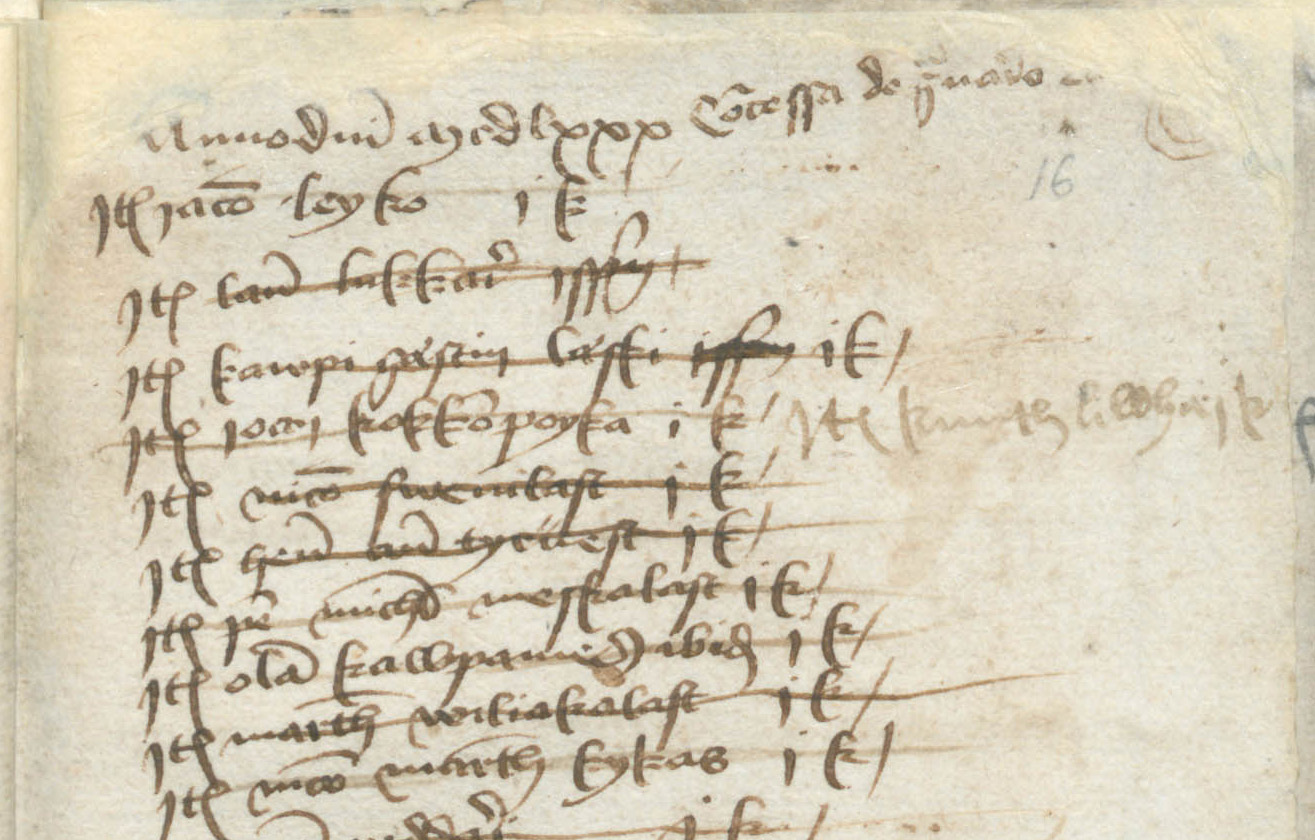
\includegraphics{pics/kalliala_fol16r.jpg}    
  \end{center}


  \vspace{5mm}

{\raggedright {\fontsize{15}{18}\fontspec{Aboensis}Annodnĩ \abroman{1480} Cõcessa de [ger]*nario ec
  \\
  \abl{\abitem{} jacõ leyko \hspace{0.7cm} i k,}
  \abl{\abitem{} laũ lukkari \hspace{0.3cm} i span, }
  \abl{\abitem{} kawpi gästin läski i span i karp, }
  \abl{\abitem{} joan kokkopoyka \hspace{2mm} i k, {\color{brown!75}\abitem{} knuth liwha i k} }
  \abl{\abitem{} nicõ swenilast \hspace{0.3cm} i k, }
  \abl{\abitem{} he~n an~d tyrwest i k, }
  \abl{\abitem{} pe[der] michlss meskalast i k, }
  \abl{\abitem{} olã kawpamies ibi/d i k, }
  \abl{\abitem{} ma~th wiliakalast i k, }
  \abl{\abitem{} nicõ marthensz kykas i k, }
}}
\caption{Year 1480 in Kalliala parish granary accounts.
  \emph{Kallialan kirkontilit, Valtionarkisto, folio 16r.}}
  \label{fig_kalliala}
\end{figure}

\begin{quote}
{
  \raggedright
  Anno domini MCDLXXX Concessa de
  granario ec \emph{kalliala}\\
  Item Jaco\emph{b} Leyko \hspace{0.7cm} i k\emph{arp} \\
  Item Lau\emph{ri} Lukkari \hspace{0.3cm} 1 span \\
  Item Kauppi-Kestin leski 1 span 1 karp \\
  Item Johan Kokkopoika \hspace{2mm} 1 k\emph{arp}, Item Knuth Liuha i
  k\emph{arp} \\
  Item Niko\emph{laus} Sveniläst \hspace{0.3cm} 1 k\emph{arp} \\
  Item Hen\emph{rik} And\emph{ersson} Tyrvääst  1 k\emph{arp} \\
  Item Ped\emph{er} Mich\emph{e}lss\emph{on} 1 k\emph{arp} \\
  Item Ola\emph{us} Kauppamies ibid\emph{em}  1 k\emph{arp} \\
  Item Ma\emph{theus} Viljakalast 1 k\emph{arp} \\
  Item Niko\emph{laus} Marthensson Kykas 1 k\emph{arp} \\
}

\end{quote}



\subsection{The account book of Olaf Nilsson Tawast}\label{sec_tavast}

Olaf Nilsson (Tawast) (c. 1400–1460) belonged to the Finnish nobility
and the base of his power was in Tavastia where he was first a judge
from c. 1433 and the castellan of Häme Castle from 1455. He was the
nephew of Bishop Magnus Olai (Tawast) of Åbo Diacose and a supporter
of King Karl Knutsson (Bonde). Their patronage helped Olaf to greatly
enlarge his holdings in Tavastia. His book of household accounts has
survived.

Figure \ref{fig_olaf_nilsson} has a snippet gives details of a land
sale circa 1455.

\begin{figure}

  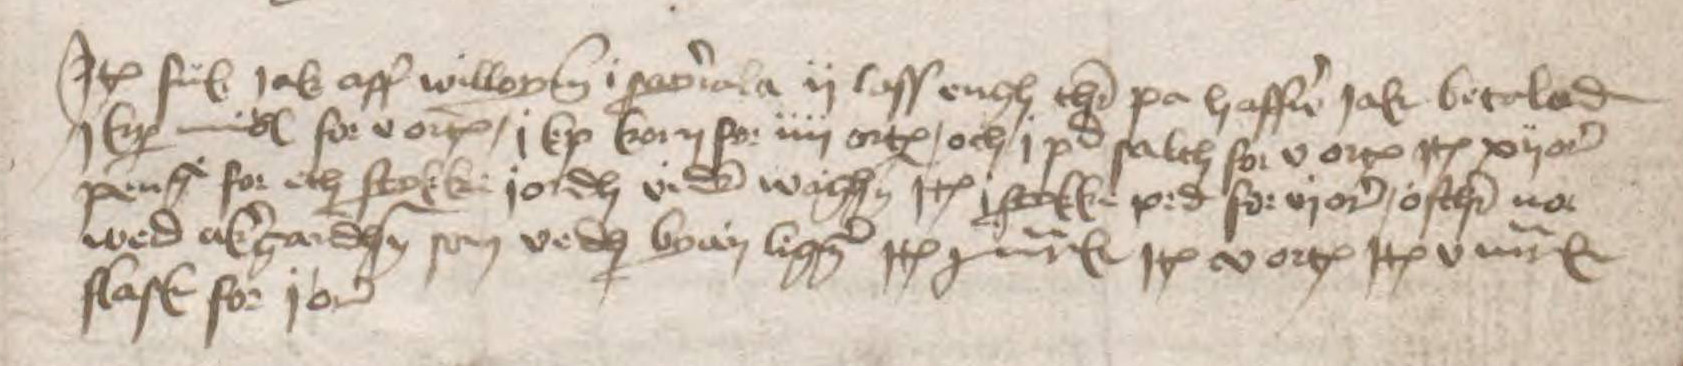
\includegraphics{pics/DF3001_fol2r.jpg}

  \vspace{5mm}

  {\raggedright {\fontspec{Aboensis}\fontsize{16}{20}\selectfont
      \abl{\noindent \abitem{} fik iak aff willoyn i sayriala ii lass
        engh t*hz pa haffure jak}
      \abl{betalad t*hz pa haffure jak betalad j \abkarpio{} miöl for v \abortug, i \abkarpio{} korn}
      \abl{for iiii \abortug{} och i \abpund{} salch for v \abortug.
        \abitem{} xii \abore{} \abpenning{} for eth stykke }
      \abl{jordh vidher wäghen. \abitem{} i stykke jord for vi
        \abore{}, öster nor wed }
      \abl{aker gardhen som vedh byen ligghre \abitem{} \abroman{0.5}
        \abmark{}, \abitem{} v \abortug{}, \abitem{}}
      \abl{v \abmarc{} fläsk for i \abore}}}

  
  \caption{Snippet from accounts of Olaf Nilsson Tawast, c. 1455. \emph{DF
    3001, SDHK 43935, Riksarkivet codices C 38, folio r2r}}
  \label{fig_olaf_nilsson}
\end{figure}

\begin{quote}
Jtem fik iak aff Willoyn j Sayriala ij las engh; ther pa hafwer iak
betalat j karp miøl for v ortuger, j karp korn for iiij ortuger ok j
pund salt for v ortuger, jtem xij öre peninga for j stykke jordh
widher wæghen, jtem j stykke jordh for vj øre østher nor wedh aker
gardhen, som wedh byen liggher, jtem 1/2 mark, jtem v ørtuger, jtem
v mark flæsk for j øre.
\end{quote}

\begin{quote}
  Item I received a 2 lass meadow from Willoyn of Sairiala; for which I
  paid 1 karp flour valued at 5 ortuger, 1 karp barley at 4 örtuger
  and 1 pund salt at 5 örtuger. Item 12 öre in coins for one piece of
  land next to road, item 1 piece of land for 6 öre to East of field
  that is next to the village, item 1/2 mark in coins, item 5 örtuger,
  item 5 marks of pork at 1 öre.
\end{quote}


\subsection{Table of contents of \emph{Konunx balker}}

Each chapter of \emph{Codex Aboensis} starts with a table of contents
of that chapter. Figure \ref{fig_kunnunx_contents} shows the beginning
of the \emph{Konunx balker}.

\begin{quote}
  Här byrias konungx balker ok tälias y honom flokkar fyra ok trätigh
  item \\

  \begin{tabular}{lp{10cm}l}
    ¶ & Wm suerikis konungx rike kuilket i sik haffue siw biscops döme
    och nio lagmanz döme & 1 \\
    ¶ & Offuer akth suerike ager ey konunglixlik krona och ei knongher
    wtan een wara & 2 \\
    ¶ & Ey ma konungher minsca kronunnan räth firi androm konunghe & 3
    \\
    ¶ & Yn är til koningxrikit i suerike konungr wäliandhe och ey
    ärffuandhe & 4 \\
    ¶ & Tesse ärä nonungx edha först ath han scal elsca gud och the
    helghä kirkio och agher edh syn suäria aa book och helgho doma & 5 \\ 
  \end{tabular}
\end{quote}



\begin{quote}
  Here begings the Kings Beam that contains four and thirty items  \\

  \begin{tabular}{lp{10cm}l}
    ¶ & On the King's realm of Sweden that has seven diacoses and nine
    judicical districts & 1 \\
    ¶ & There is only one king's crown and one king over the Sweden & 2\\
    ¶ & The king may not diminish the crown's income from later
    kings & 3 \\
    ¶ & The kingship in Sweden is by election and not inherited  & 4 \\
    ¶ & This is the king's oath: to love God and the Holy Church and
    to swear by the Bible and holy relics & 5 \\ 
  \end{tabular}

\end{quote}

\begin{figure}


  \begin{center}
    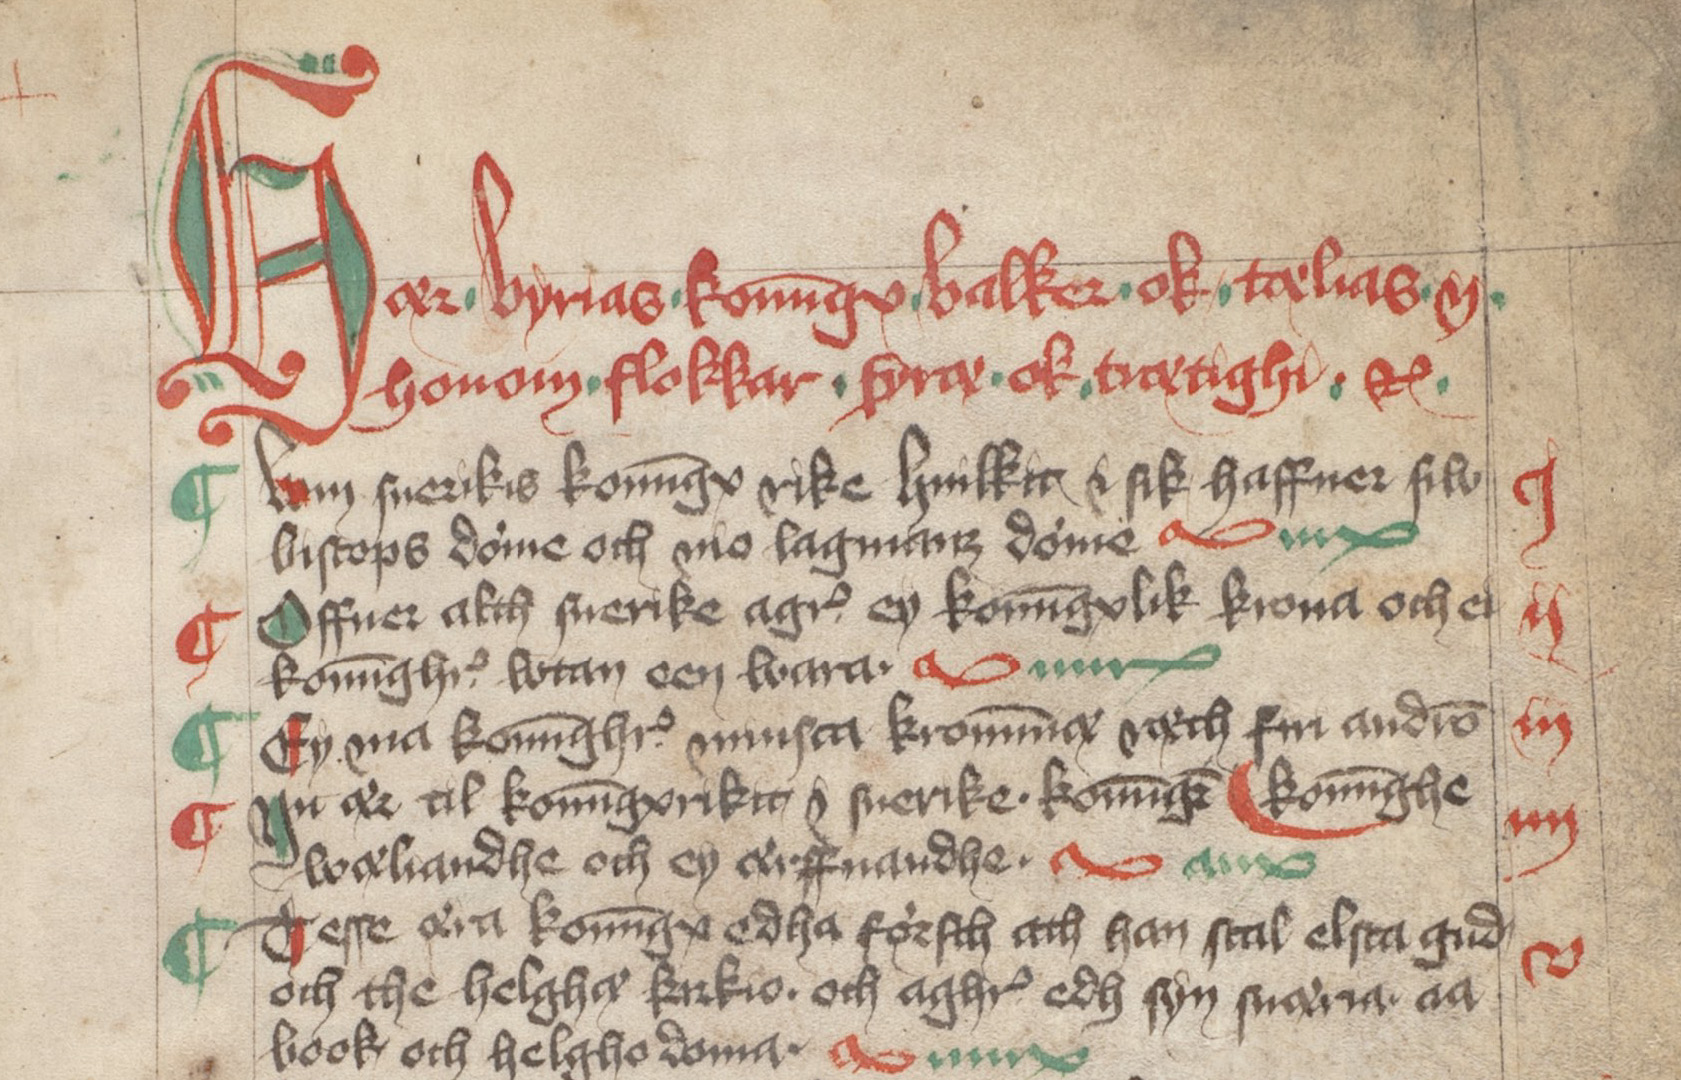
\includegraphics[width=10cm]{pics/kununx_balk.jpg}    
  \end{center}


% Codex aboensis, folio 22 r. 
\newcommand{\gc}{\abgreen{·}}
{{\fontspec{Aboensis}\fontsize{18}{18}\selectfont\raggedright
      \abstartchaptertwowithpos{H}{1.1}{-2mm}{-2mm}{\abrubric{är\gc{}byrias\gc{}kon~ugx\gc{}balker\gc{}ok \gc{} tälias\gc{}y\gc{}}}%
      {\abrubric{honom\gc{}flokkar{}\gc{}fyra \gc{} ok \gc{} trätigh \gc{}\abitem\gc}}

    \fontsize{15}{17}\selectfont

    \begin{tabular}{l@{ }l@{ }l}
      \abb{\abparaother} & 
      \abb{\abcapital{W}*m suerikis kon~ugx rike huilket i sik haffue} 
      & \abb{\abrubric{I}} \\
      & \abb{siw biscops döme och nio lagmanz döme \abred{!} \abgreen{**<}}  \\
      \abb{\abpara}  
      & \abb{\abcapitalother{O}ffuer akth suerike ager ey kon~ugxlik
        krona och } 
      & \abb{\abred{ii}} \\
      & \abb{ei kon~ugher wtan een wara \abred{!} \abgreen{******<}} &  \\
      \abb{\abparaother} & \abb{\abcapital{E}y ma kon~ugher minsca
        kronuñä räth firi} & \abb{\abred{iii}}   \\
      & \abb{andrõ kon~ughe \abred{!} \abgreen{!****<}} \\
      \abb{\abpara}
      & \abb{\abcapitalother{Y}n är til kon~igxrikit i suerike.
        kon~ug~r wälia} 
      & \abb{\abred{iiii}} \\
      & \abb{ndhe och ey ärffuandhe \abred{!} \abgreen{!*****<}}  \\
      \abb{\abparaother} &
      \abb{\abcapital{T}esse ära kon~ugx edha försth ath han scal} 
      &\abred{v} \\
      & \abb{elsca gud och the helghä kir:kio. och agher edh} & \\
      & \abb{syn suäria aa book och helgho doma.  \abred{!} \abgreen{\_***<} }  \\
    \end{tabular}
    
}}

\caption{The beginning of table of contents of \emph{Konungx balker},
  \emph{Codex Aboensis folio 22 r.}}
\label{fig_kunnunx_contents}  
\end{figure}



\subsection{The rules of noble service}\label{sec_noble_service}


\begin{figure}
  \centering
  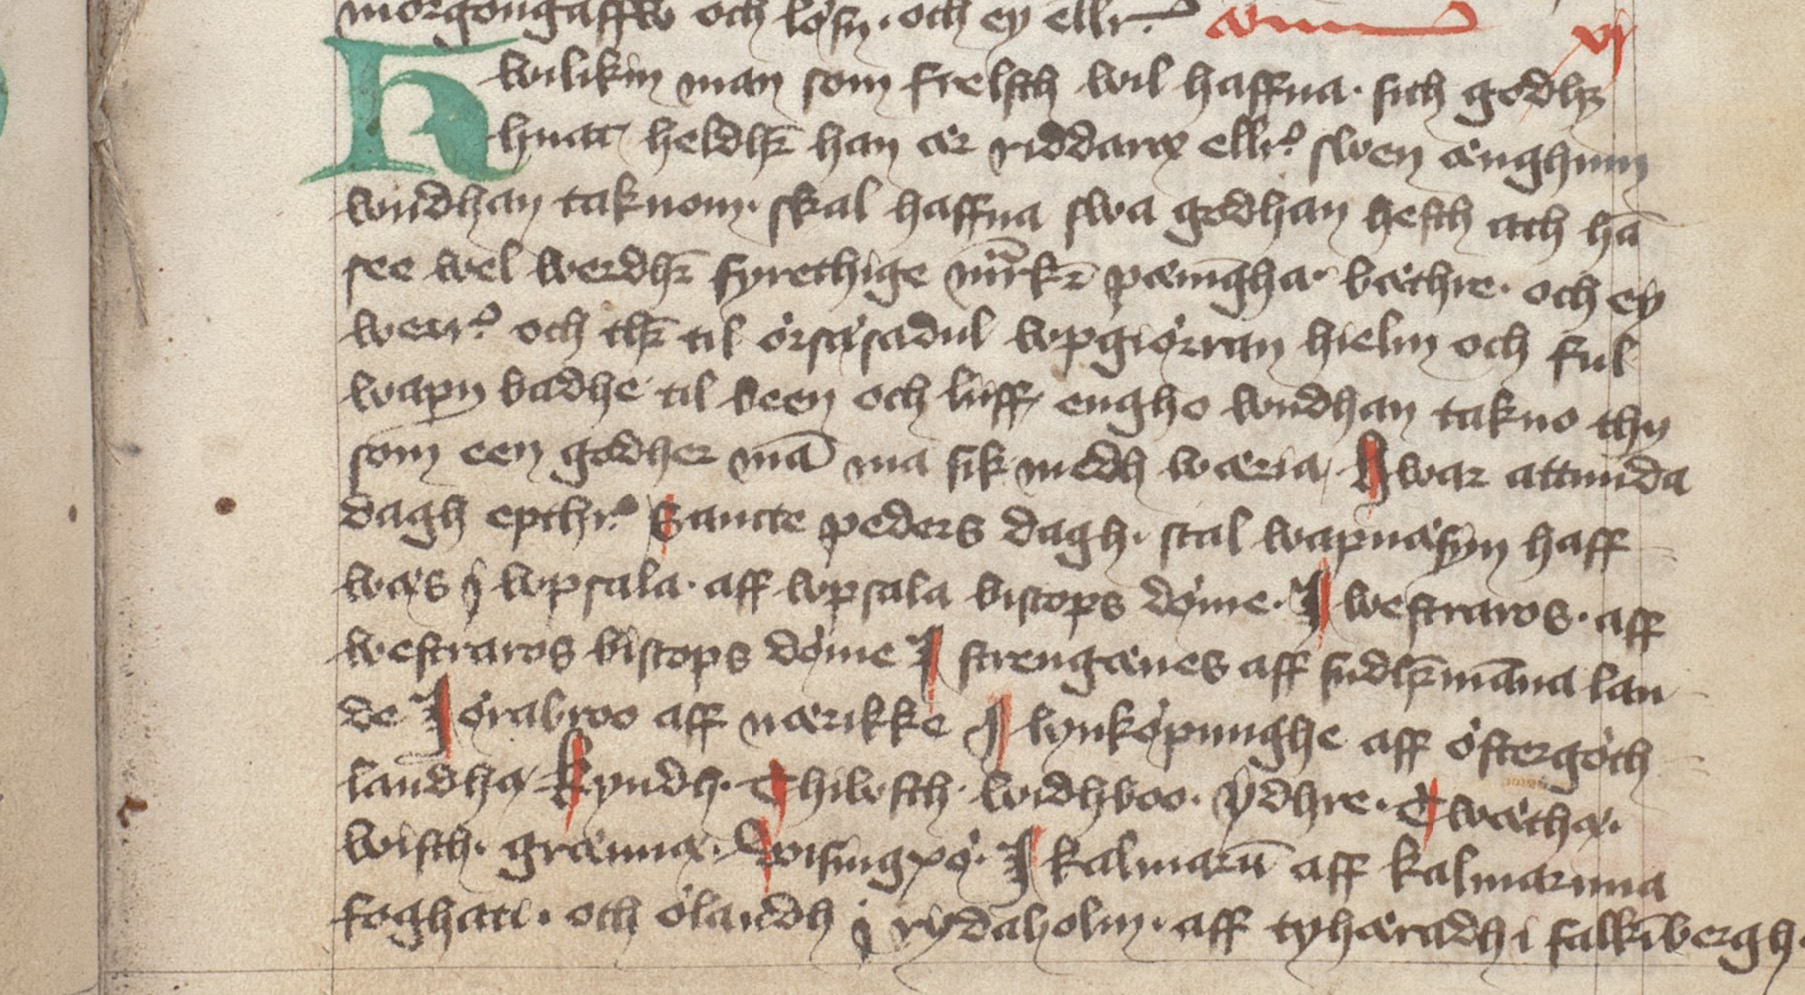
\includegraphics[width=12cm]{pics/aboensis-27r.jpg}

  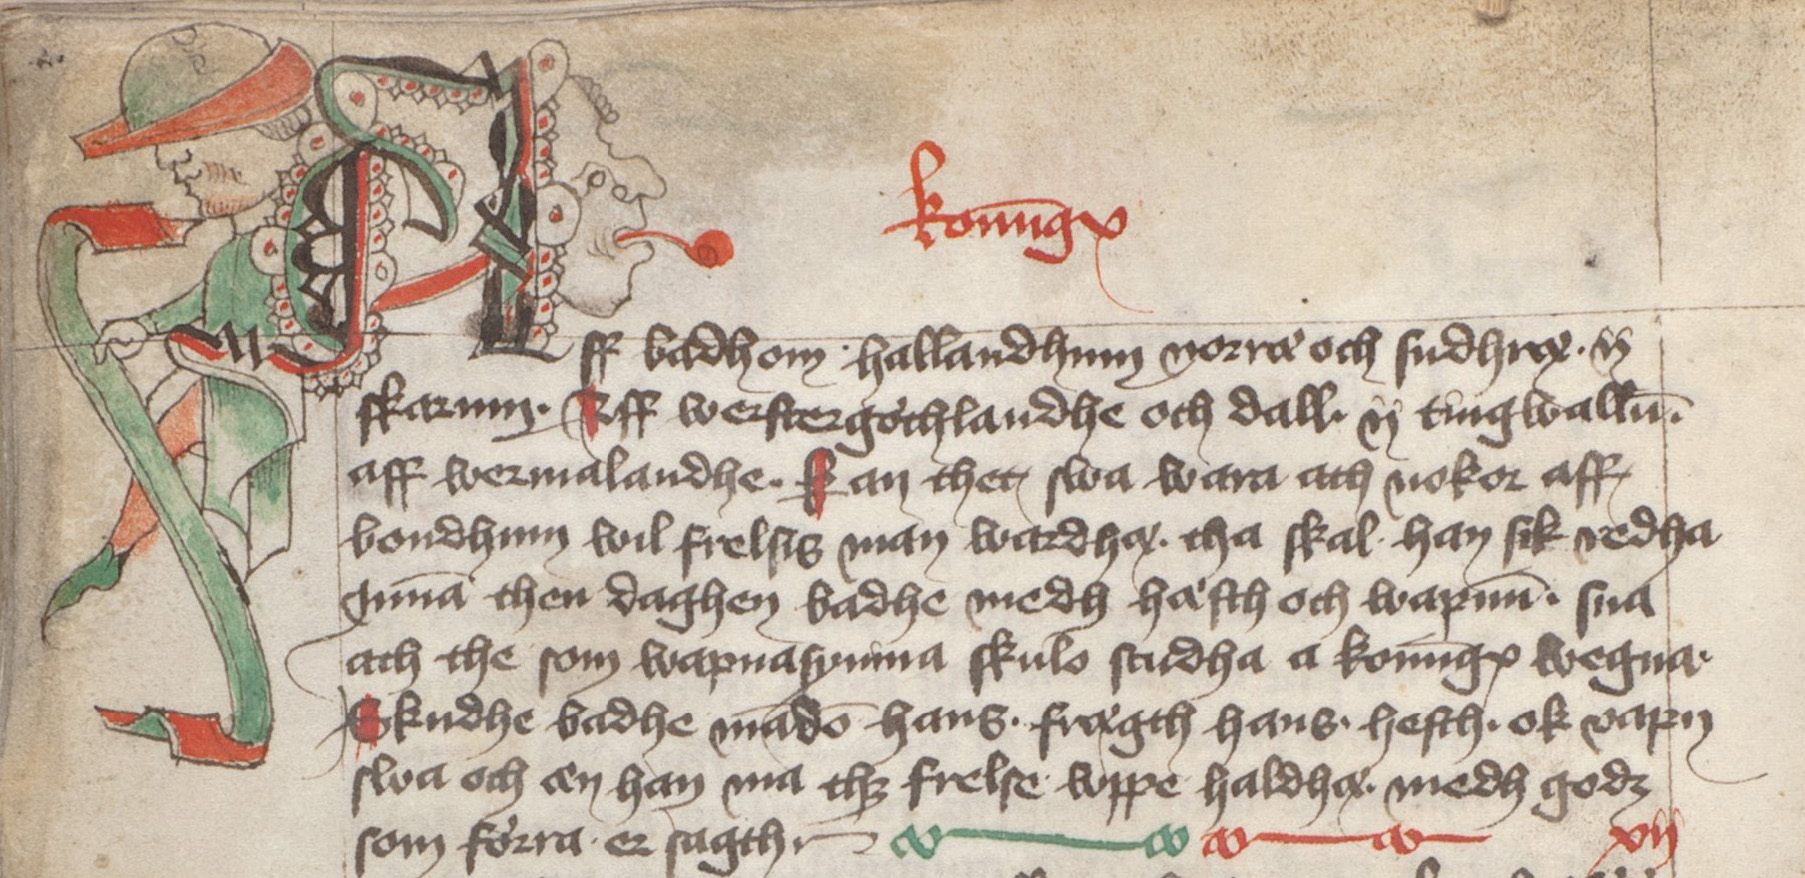
\includegraphics[width=12cm]{pics/aboensis-27v.jpg}

  \caption{The rules of noble service in \emph{Konungx balker} in
    \emph{Codex aboensis}. Note how the initial of \emph{aff} occurs
    in the middle of sentence.}\label{fig_konungx_service}
\end{figure}

During the middle ages the borders of Swedish noble class were fluid.
Being a noble was not yet officially hereditary but instead it was
tied to service as a man-at-arms. In practice, powerful families had
noble status from generation to generation but but the door was still
open for a common peasant to rise to the ranks of nobles.

The core concept was that of \emph{frälse} – freedom from paying
taxes. This could be obtained by equipping a man-at-arms to serve in
the king's army. The men-at-arms were divided into \emph{riddare} and
\emph{sven}, knights and squires. 

The \emph{Konunx balker} lists the required equipment and establishes
the dates of annual inspections of the nobles in the section 11.

\begin{figure}
% Codex aboensis, folio 27 r. 
{{\fontspec{Aboensis}\fontsize{15}{18}\selectfont\raggedright
    \abstartchapterother{H}{wilikin man som frelsth wil haffua. sith
      godhz}{
      huat heldlsz han är riddarä eller swen änghnin }
    \abl{wiidhan taknom. skal haffua swa godgan hesth ath h~a }
    \abl{see wel werdhs fyrethige \abmark{} päni~gha. bäthre och ey }
    \abl{weier och thz til örsäsadul wpgiörran hielm och fulwa~p}
    \abl{badhe til been och liiff, engho wudhan takno thz som }
    \abl{e~e gadher mã ma  sik niedh wäria. \abcapital{H}war att~uda dagh}
    \abl{epther \abcapital{S}ancte peders dagh. scal wapnäsyn haff wäs i }
    \abl{wpsala. aff upsala biscops döme. \abcapital{I} westraros. aff wes}
    \abl{tra ros  biskops döme \abcapital{I} strengänes aff sudh~rmanna }
    \abl{lande \abcapital{I} örabroo aff närikke \abcapital{I} lynköpinghe aff öster-}
    \abl{göth landha  \abcapital{K}*yndh. \abcapital{T}hiwsth.  widhboo. Ydhre. \abcapital{T}wä-}
    \abl{thä. wistho grännä. \abcapital{W}isixö. \abcapital{I} kalmrarun aff kal-}
    \abl{mar~na foghate. och ölaidh i  rydaholm. aff tyhäradh }
    \abl{i falk~ibergh. aff badhom  hallandh~u norrä och sudhrä. }
    \abl{y skarum. \abcapital{A}ff werstergöth  landhe oh dall y tiugwall~u. }
    \abl{aff wermalandhe.  \abcapital{K}an thet  swa wara ath nokor aff,}
    \abl{bondhum wil frelsis  man wardha.  tha skal han sik }
    \abl{redha innã then daghen badhe medh  hästh och wapn~u. }
    \abl{swa ath the som wapnasynna skuld skudha  a konu~gx  }
    \abl{wegna. \abcapital{S}kundhe badhe mandõ hans. fräght  hans}
    \abl{hesth. ok   wipen swa och än han ma thz frelse wppe  hal}
    \abl{dhä. medh godz som   förra ez saght. \abgreen{!>>>***>>>!} }}}
\caption{The requirements of noble service in \emph{Konungx balker},
  \emph{Codex Aboensis folio 27 r.}}
  
\end{figure}


\begin{quote}
  Hwilikin man som frelsth wil haffua. sith godhz huat heldlsz han är
  riddarä eller swen änghnin wiidhan taknom. skal haffua swa godgan
  hesth ath hã see wel werdhs fyrethige markea päningha. bäthre och ey
  weier och thz til örsäsadul wpgiörran hielm och fulwapn badhe til
  been och liiff, engho wudhan takno thz som een gadher man ma sik
  niedh wäria. Hwar attunda dagh epther Sancte peders dagh scal
  wapnäsyn haff wäs i wpsala aff upsala biscops döme. I westraros. aff
  westraros biskops döme. I strengänes aff sudhermanna lande. I
  örabroo aff närikke. I lynköpinghe aff östergöthlandha, Kyndh,
  Thiwsth, widhboo, Ydhre. Twäthä. wistho grännä. Wisixö. I kalmrarum
  aff kalmarnna foghate. och ölaidh i rydaholm. aff tyhäradh i
  falkinbergh. aff badhom hallandhum norrä och sudhrä. y skarum. Aff
  werstergöthlandhe oh dall y tiugwallun. aff wermalandhe. Kan thet
  swa wara ath nokor aff, bondhum wil frelsis man wardha. tha skal han
  sik redha innan then daghen badhe medh hästh och wapnum. swa ath the
  som wapnasynna skuld skudha a konungx wegna. Skundhe
  badhe mandõ hans. fräght hans hesth. ok wipen swa och än han ma
  thz frelse wppe haldhä. medh godz som förra ez saght.
\end{quote}


\begin{quote}
  He who wants to have noble privileges for his properties, be he a
  knight or a squire, without forgetting anyone, should have a horse
  worth 40 marks in coins or more, but not less, and a war saddle,
  good helmet, armor for limbs and body and weapons with which a good
  man can defend himself.  

  Each year on the eight day after the Saint Peter's day there is an
  inspection of arms in Uppsala for the whole diacose of Uppsala, in
  Västerås for the Västerås diacose, in Strängnäs for Södermanland, in
  Örebro för Närke, in Linköping for Östergötaland, Kinda, Tjust,
  Vedbo, Ydre, Gränna, Tveta, Vista and Visingö, in Chalmers for the
  Chalmers bailiff county and Öland, in Rydaholm for Tiohäräd, in
  Falkenberg for North and South Halland, in Skara for Västergötaland
  and Dal, in Tingvalla for Vermland. 

  If a peasant wants to become a noble man he much obtain a horse and
  weapons before that day so that those who inspect the arms for the
  king can check his manliness and fitness, his horse and weapons, and
  whether he can support his armed service with his properies. 

\end{quote}

The King Kristofer's \emph{The Laws of the Realm} from the 15th
century have the same rules expressed in almost the same form. The
enigmatic \emph{Herra Martti}\footnote{Probably Martinus Olai, the
  priest of Stockholm's Finnish concegration but that is not certain.}
translated Kirstofer's laws to Finnish in 1540s. His translation is
typeset to \Aboensis{} in figure \ref{fig_martti}. 

\begin{figure}
  \begin{minipage}{14cm}
  {\fontspec{Aboensis}\fontsize{15}{19}\selectfont\raggedright
    \noindent\abstartchapter{I}{Oca mies wapautta tacto hänen hyfuydhens, mikä hän on }{%
      \abcapital{R}iddari taicka \abcapital{S}wenni, ei yctäken eroittadhen, hänen pitä }
    \abl{hyfuydhens crvnvn palueluxen tekemen, ia idze pitämen nijn}
    \abl{hyfwen hewoisen, että hän maxa 40 \abmark{} \abcapital{R}uotzin pe~ngeitä,}
    \abl{pareman ia ei paheman, sihen mös täydhet odhatt se rwmin }
\abl{että jalkain pällä, ei mitän eroittadhen, sen iälkin, quin hyfwä } 
\abl{mies machta idzens wariella. \abcapital{J}oca wuosi wijkon peräst \abcapital{S}ant }
\abl{petarin päiven, pitä kilpein katzelmuxen olemen. \abcapital{W}*psalos cai-  }
\abl{kest \abcapital{W}*psalon \abcapital{P}ispan hijppacu~nast; wästeråxes, wästråxen hijppa }
\abl{cu~nast; \abcapital{S}tregnäisis  \abcapital{S}ödermannin maalda, \abcapital{Ö}*r:ebros, \abcapital{N}ärikäst, }
\abl{\abcapital{J}äneköpungis, \abcapital{Ö}stergöthin maalda,  \abcapital{K}ijnd, \abcapital{T}iust, widbro, \abcapital{I}dra, }
\abl{\abcapital{T}veta, wistgräna, \abcapital{W}isingzöö, \abcapital{K}almarisa, fogdi ia \abcapital{Ö}landimaa, }
\abl{\abcapital{R}idbåholmis, \abcapital{T}ijhan kihlac~uda, falckenbäris, molemist \abcapital{H}ållan}
\abl{deist, sekä pohia että \abcapital{E}telä, \abcapital{S}kara wästergöthin maalda ia }
\abl{\abcapital{D}alast, \abcapital{T}ingwallist, wärmlandis; \abcapital{T}urgusa caickelda \abcapital{S}uomen* }
\abl{malda. \abcapital{J}os nijn taita tapachtu että ioku talonpoijst tacto tulla }
\abl{wapadex nijn tule hän itzens walmista ennen tätä päiwä sekä }
\abl{hewoisen että odhain cansa. \abcapital{N}*ijn että ne quin kilpen cadzelmust }
\abl{pitä pitämen kuningan puolest, että he näkevet sekä henen }
\abl{miehudens woiman että hewoisen ia odhat ia ios hän woipi sen }
\abl{wapaudhen ylöspitä hyfwydellä. \abcapital{C}aicki pitä wapadhet miehet}
\abl{kilpein \abcapital{C}adzelmuxella tuleman, ia ioka mies nijn \abcapital{R}iddarit quin  }
\abl{\abcapital{S}wennitkin heidhen harniskans pälle~s wetämen, ia idze cukin }
\abl{oman hewoisens pälle istuman, walmistettun hewoisen ia kilpein }
\abl{cansa quin io edhellä on sanottu.}
}
    
  \end{minipage}

  \caption{The same paragraph from the \emph{Kunungx balker} of the
    King Kristofer's \emph{Laws of the Realm} in a 1540s Finnish
    translation of the law by Herra Martti (B 96, f.2r)}
  \label{fig_martti}
\end{figure}


\begin{quote}
  Ioca mies wapautta tacto hänen hyfuydhens, mikä hän on Riddari
  taicka Swenni, ei yctäken eroittadhen, hänen pitä hyfwydhestens
  crvnvn palueluxen tekemen, ia idze pitämen nijn hyfwen hewoisen,
  että hän maxa 40 ma\emph{rca} Ruotzin penningeitä, pareman ia ei
  paheman, sihen mös täydhet odhatt se rwmin että jalkain pällä, ei
  mitän eroittadhen, sen iälkin, quin hyfwä mies machta idzens
  wariella. Joca wuosi wijkon peräst Sant petarin päiven, pitä kilpein
  katzelmuxen olemen. Wpsalos caikest Wpsalon Pispan hijppacunnast;
  wästeråxes, wästråxen hijppacunnast; Stregnäisis Södermannin maal\-da,
  Örebros, Närikäst, Jäneköpungis, Östergöthin maalda, Kijnd, Tiust,
  widbro, Idra, Tveta, wistgräna, Wisingzöö, Kalmarisa, fogdi ia
  Ölandimaa, Ridbåholmis, Tijhan kihlacunda, falckenbäris, molemist
  Hållandeist, sekä pohia että Etelä, Skara wästergöthin maalda ia
  Dalast, Tingwallist, wärmlandis; Turgusa caickelda Suomenmalda. Jos
  nijn taita tapachtu että ioku talonpoijst tacto tulla wapadex nijn
  tule hän itzens walmista ennen tätä päiwä sekä hewoisen että odhain
  cansa. Nijn että ne quin kilpen cadzelmust pitä pitämen kuningan
  puolest, että he näkevet sekä henen miehudens woiman että hewoisen
  ia odhat ia ios hän woipi sen wapaudhen ylöspitä hyfwydellä. Caicki
  pitä wapadhet miehet kilpein Cadzelmuxella tuleman, ia ioka mies
  nijn Riddarit quin Swennitkin heidhen harniskans pälle\emph{n}s
  wetämen, ia idze cukin oman hewoisens pälle istuman, walmistettun
  hewoisen ia kilpein cansa quin io edhellä on sanottu.
\end{quote}


\subsection{Excommunication of Sääksmäki peasants}

In late 1330s there was some sort of unrest in the Sääksmäki parish
where a number of peasants refused to pay their tithes to their vicar
Henrik Harmansson. The exact cause of the issue is not known, but the
issue was important enough that Henrik himself traveled to Avignon in
Spring 1340 and obtained a bull from Pope Benedictus XII that
excommunicated the 25 peasants until they paid the tithes and a fine
of three marks for each week that they refused to pay them.

This bull is the first document in the \emph{Black Book} and it is one
of the most famous medieval documents in Finland. In particular
interest is the list of peasants that have caused a lot of speculation
about their backgrounds and roles in the society. The scribe made an
error when copying the document to the cartulary and accidentally left
two lines out of it just after the list of names, jumping from
\emph{eiusdem ecclesie} to \emph{eidem ecclesie}. Hausen filled the
missing lines for his transcription from another cartulary. 

\begin{figure}
  \centering
  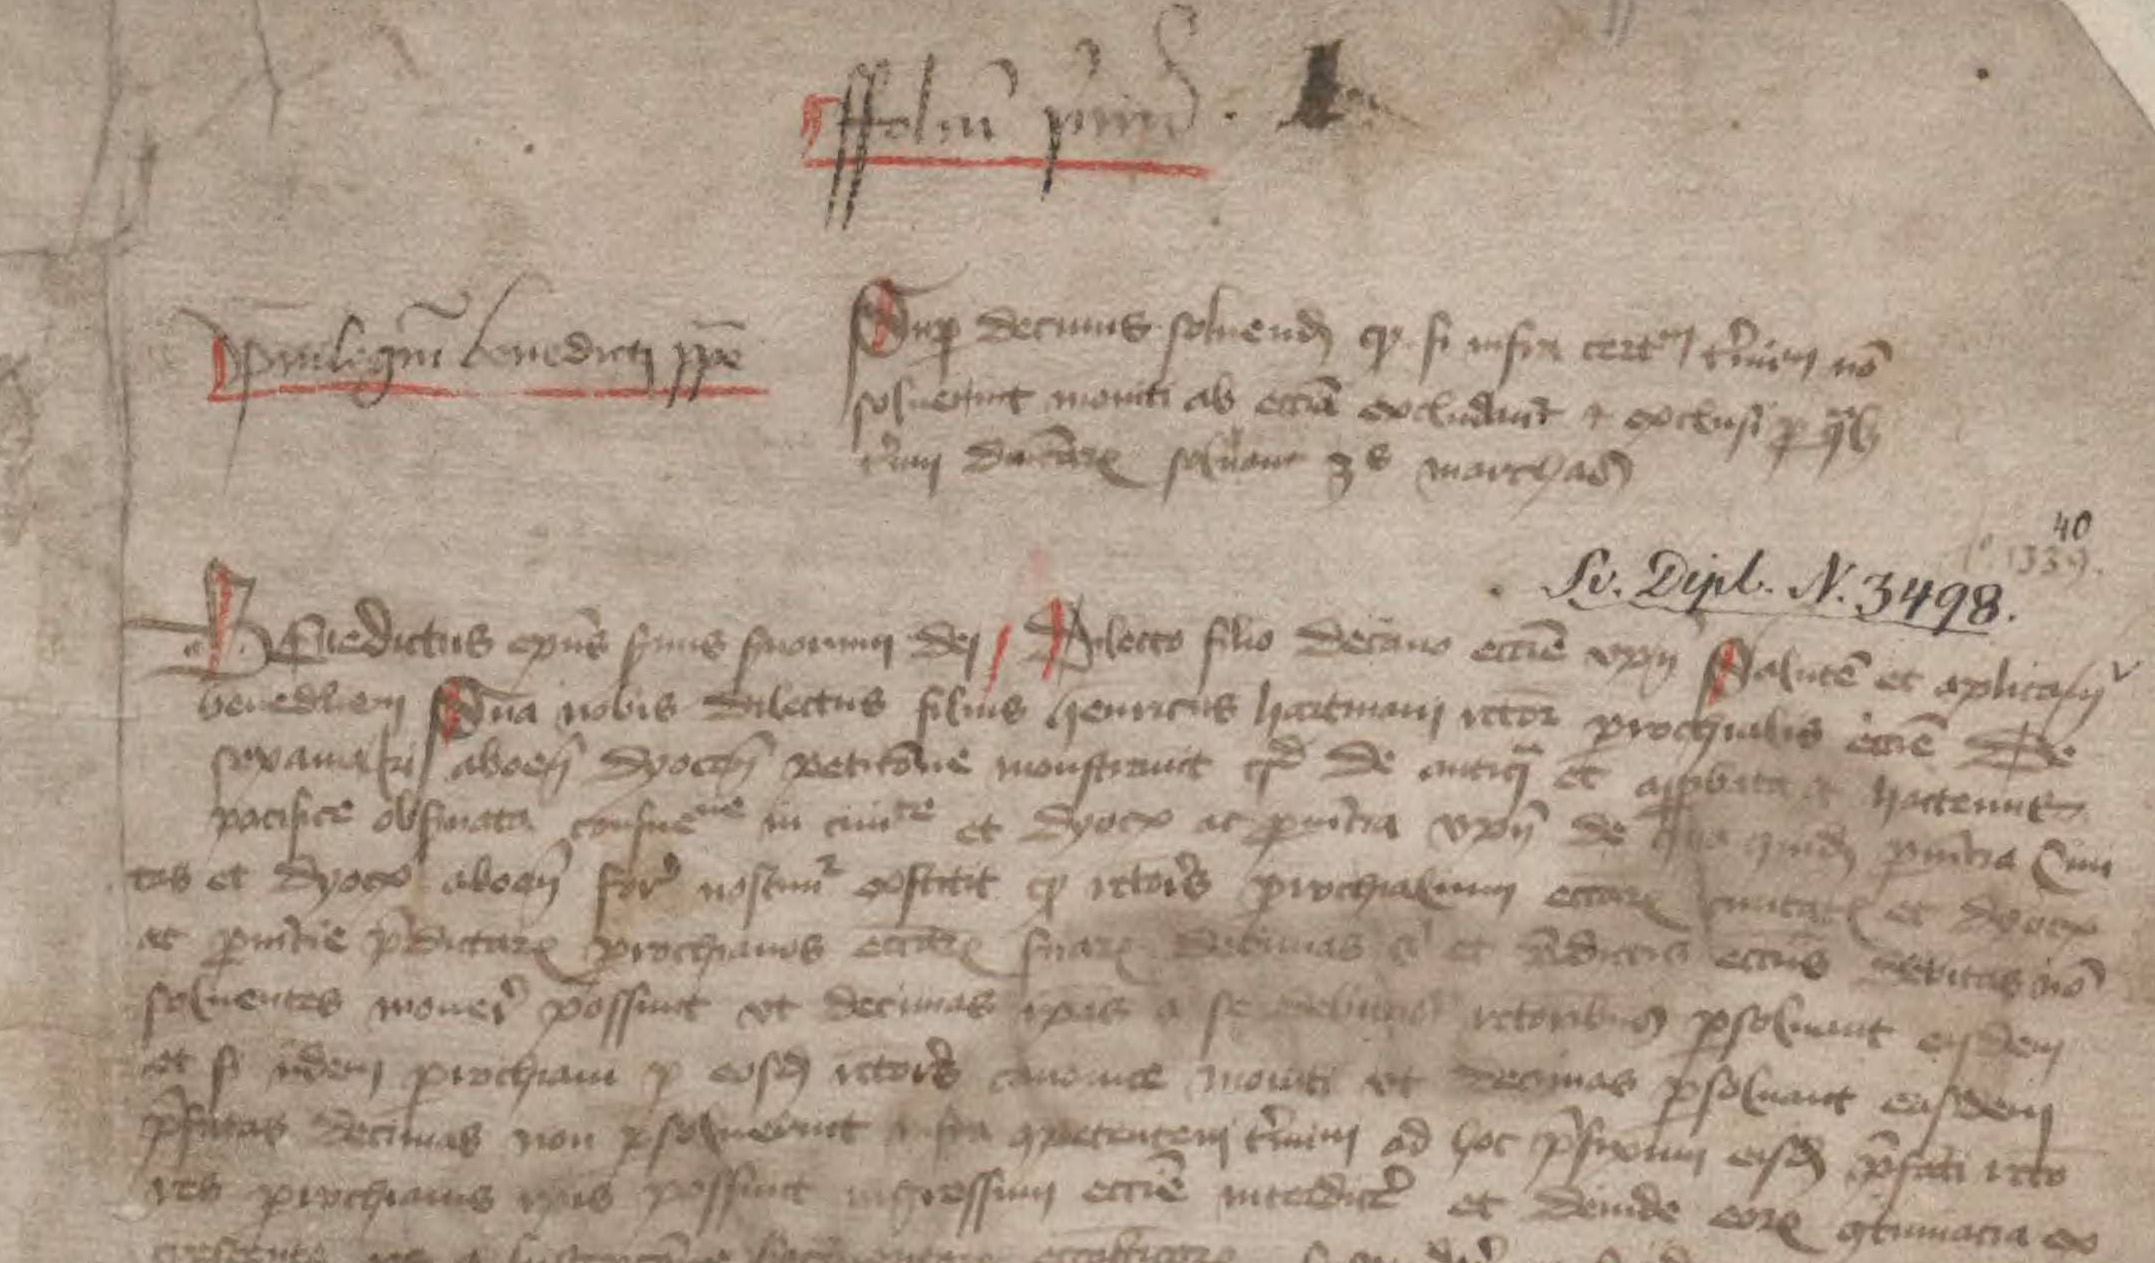
\includegraphics[width=10cm]{pics/REA-001r.jpg}
  \caption{The beginning of an excommunication letter (DF 467, REA
      99, \emph{Registrum ecclesia Aboensis f.1r.)}}\label{fig_excommunication_rea}
\end{figure}


\begin{landscape}
  \begin{figure}
    {\fontsize{15}{15}\fontspec{Aboensis}\raggedright

      \begin{tabular}{l@{\hspace{4cm}}p{10.3cm}}
        Pr~ileg~m Benedicti pp~e & \abcapital{S}u[per] decimis
          soluen/d [quod] si* infra cert`m ´tmi num n~o
          soluerint moniti ab ecci~a excludan´t \& exclusi [pro]
          [qua]ß ´tum donc~a[rum] soluant 3`s marchas
      \end{tabular}

      \vspace{1cm}

      %initialc{b}{78}{5mm}{1pt}{}
      {\abcursiveinitial{B}Enedictus ep~us ßruus ßruorum dei
        \abcapital{D}ilecto filio decano ecci~e vp~n
        \abcapital{S}alut~e et aplicam \\ bened~nem \abcapital{S}ua
        nobis dilectus filius henricus hartmani retor
        [par]rochialis ecci~e De sexamäki \\ aboe~n dyoc~e
        peticione monstrauit qd de anti[qua] et
        a[prop]bata et hactenus pacifice obßruata \\
        consue`n`e in ciui`t`e et dyo[cis] ac
        [pro]uincia vp~n de qua quidem [pro]uincia
        ciuitas et dyo[cis] aboe~n fore \\ noscu´n exstitit
        [quod] recto[re]s [par]rochialium
        eccia[rum] ciuitat[is] et dyo[cis] ac
        [pro]uincie [pre]dicta[rum]
        [par]rochianos \\ ecc~e[rum] sua[rum] .
        decimas sibi et [pre]dictis
        ecc~is debitas n~o soluentes monere possunt vt decimas \\
        ipsas a se debitas rectori[bus] [per]soluant
        eisdem et si* iidem [par]rochiani [per] eos/d
        rectores cononice \\ moniti vt decimas [per]soluant
        easdem [pre]fatas decimas non [per]soluerint
        infra [con]petentem ´tmi\\ num   ad hoc
        [pre]fixum eis/d [pre]fati rectores
        [par]rochianis ipsis possunt ingressum ecci~e 
        inter- \\ dicere et deinde eo[rum] contumacia excrescente,
        eos a suscepc~one sa´camento[rum] ecc~etico[rum]
        suspe\\ }}
    \mbox{}\vspace{5mm}\mbox{}
    \caption{The beginning of an excommunication letter (DF 467, REA
      99, \emph{Registrum ecclesia Aboensis f.1r.})}
    \label{fig_excommunication_1}
  \end{figure}
\end{landscape}


\begin{quote}
  Benedictus episcopus, seruus seruorum Dej, dilecto filio decano
  ecclesie Vpsalensis salutem et apostolicam benediccionem. Sua nobis
  dilectus filius Henricus Hartmanj, rector parrochialis ecclesie de
  Sexamæki, Aboensis dyocesis, peticione monstrauit, quod de antiqua
  et approbata et hactenus pacifice obseruata consuetudine in ciuitate
  et dyocesi ac prouincia Vpsalensi, de qua quidem prouincia ciuitas
  et dyocesis Aboensis fore noscuntur, exstitit, quod rectores
  parrochialium ecclesiarum ciuitatis et dyocesis ac prouincie
  predictarum parrochianos, ecclesiarum suarum decimas sibi et
  predictis ecclesiis debitas non soluentes, monere possunt, vt
  decimas ipsas a se debitas rectoribus persoluant eisdem; et, si
  iidem parrochiani per eosdem rectores canonice moniti, vt decimas
  persoluant, easdem prefatas decimas non persoluerint infra
  competentem terminum ad hoc prefixum, eisdem prefati rectores
  parrochianis ipsis possunt ingressum ecclesie interdicere et deinde,
  eorum contumacia excrescente, eos a suscepcione sacramentorum
  ecclesiasticorum suspendere;
\end{quote}

\begin{quote}
  Bishop Benedictus, servant of God's servants, presents the Dean of
  Uppsala church, his beloved son, with greetings and apostolic
  blessing. Or beloved son Henrik Hartmansson, vicar of Sääksmäki in
  Abo diacose has shown us with his petition that old, accepted and
  thus far peacefully followed custom of Uppsala province that was the
  origin of Abo province, district, and diocese, has been that the
  vicars of parish churches in the said province, district, and
  diocese, can urge their parishioners who do not pay their tithes to
  the their churches, to pay their said tithes to the said vicars. And
  if the said parishioners do not after the vicars remind them to pay
  the tithes according to the canon law, still do not pay the said
  tithes in due time, the said vicars can prohibit the said
  parishioners from entering the church and thus prevent them, when
  their defiance increases, form participating from ecclesiastical
  sacraments.
\end{quote}


\begin{landscape}
  \begin{figure}
    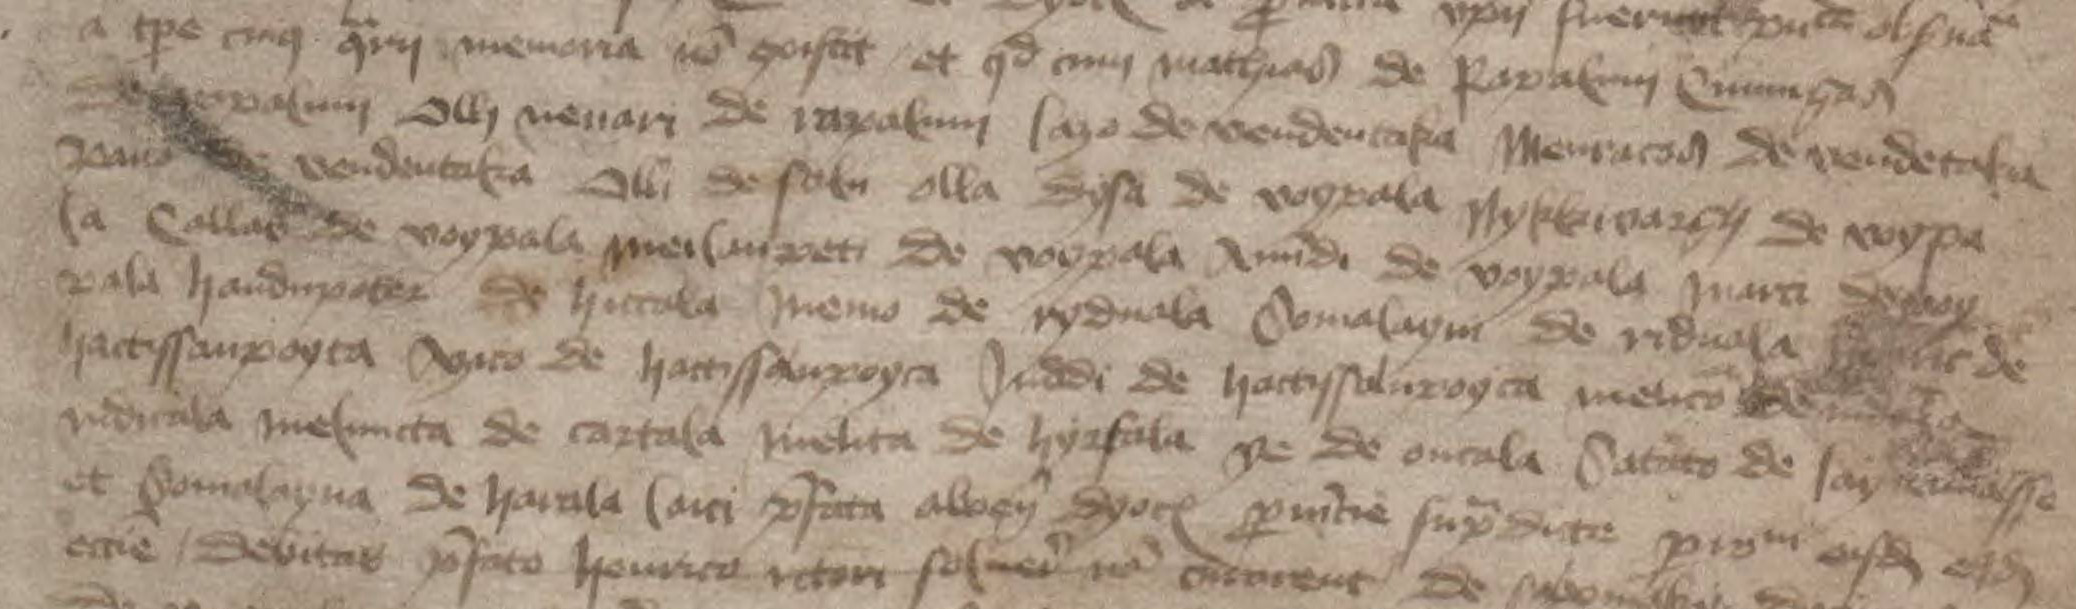
\includegraphics{pics/REA-001r2.jpg}

  {\fontspec{Aboensis}\fontsize{15}{19}\selectfont\raggedright
     \abl{a t[por]e, cuius [con]~rij memoria n~o existit, et
       qd cum mathias de Rapalum, Cuningas }
     \abl{de rapalum ollj neuari de rapalum lazo de vendentaka Menracas de vendetaka pauo}
   \abl{de vendentaka olli de salu olla dysa de voypala Nykkivargh de voypala Callas de voypala, }
   \abl{meilanpeti de voypala, an~udi de  voypala, marci \strut{}de voypala, Handupoter de hiccala memo}
   \abl{de ryduala  Somalayni de riduala, henric de hactissanpoyca Azico de hactissänpoyca}
   \abl{Juddi de hactissänpoyca, melico de iudicala meluncta de cartala, melita \strut{} de hyrfala,}
   \abl{ye de oncala Satato de Laynamässe et Somalayna de harala laici [pre]fata aboens[is] dyo[cis]}
   \abl{ [pro]uincie su[per]dicte, [par]ia`n`i eius/d ecci~e,  debitas [pre]fato henrico retori soluere nõ}}
    
    \caption{The list of excommunicated peasants (DF 467, REA
      99, \emph{Registrum ecclesia Aboensis f.1r.})}
    \label{fig_excommunication_2}
  \end{figure}
\end{landscape}



\begin{quote}
  a tempore, cuius contrarij memoria non existit, et quod, cum Mathias
  de Rapalum, Cuningas de Rapalum, Ollj Neuari de Rapalum, Lazo de
  Vendentaka, Menracas de Vende[n]taka, Pauo de Vendentaka, Olli de
  Salu, Olla Dysa de Voypala, Nykki Vargh de Voypala, Callas de
  Voypala, Meilanpeti de Voypala, Anundi de Voypala, Marci de Voypala,
  Handupoter de Hiccala, Memo de Ryduala, Somalayni de Riduala,
  Henric de Hactissanpoyca, Azico de Hactissænpoyca, Juddi de
  Hactissænpoyca, Melico de Iudicala, Meluncta de Cartala, Melita de
  Hyrfala, Ye de Oncala, Satato de Laynamæsse et Somalayna de
  Harala, laici prefata Aboensis dyocesis prouincie supradicte,
  parrochiani eiusdem ecclesie [ \textellipsis ] debitas prefato
  henrico retori soluere non
\end{quote}




\subsection{The charter of the Viborg town}

The Viborg Castle was built at the site of an old Karelian trading
center starting from 1293. It is possible that there was an older
wooden fortification in the site. During the next century the
settlement to the South East of the castle grew up to be a town. King
Eric Pomeranian (1381–1459, reigned in Sweden 1396–1434, 1434–1439)
issued a charter of privileges to the town in 1403.


\begin{quote}
  
Wy Eric, meth Gudz nadh Swerikes, Danmarks, Norghes, Wendes oc Godes
konung oc hertugh i Pomeren, kunnogt gyørom thet meth thætte wart opne
breff allom mannom swa the nu ære som the hær æpter komme scule, at wy
hafwom ont oc gifuet ware borgher, som bygge oc bo i war kyøpstadh
Wyborgh, stadz ræt æpter thy som stadz boghene i Upsalom utwyser. Thy
forbyuthom wy allom warom foghedom oc æmbetzmannom oc allom androm e
ho the hælzt æren, at hindre thom i naghre made hær amot, swa frampt
the wyliu wart hylle hafue oc war hefnd fly. In euidenciam premissorum
secretum nostrum presentibus duximus appendendum. Datum in castro
nostro Wyborgh, anno Domini m°cd°tertio, dominica infra octauam
assumpcionis virginis gloriose.

\end{quote}


\begin{quote}
  We Eric, by God's Grace the King of Sweden, Denmark, Norway, Wends
  and Goths and Duke of Pomerania, proclaim with this open letter to
  all people, both those who are no alive and those who will come
  later, that we have granted and bestowed those of our burghers who
  live in the town of Viborg the same town rights as the charter of
  the Uppsala town decrees. Thus we forbid all our bailifs and
  officials and everyone else, whoever they may be, from preventing
  them in any way against this letter if they want to enjoy our favor
  and avoid our punishments. Dated in our castle Viborg AD 1403 on the
  Sunday following the Assumption of the Glorious Virgin.
\end{quote}

\begin{landscape}
  \begin{figure}  
    \begin{center}
      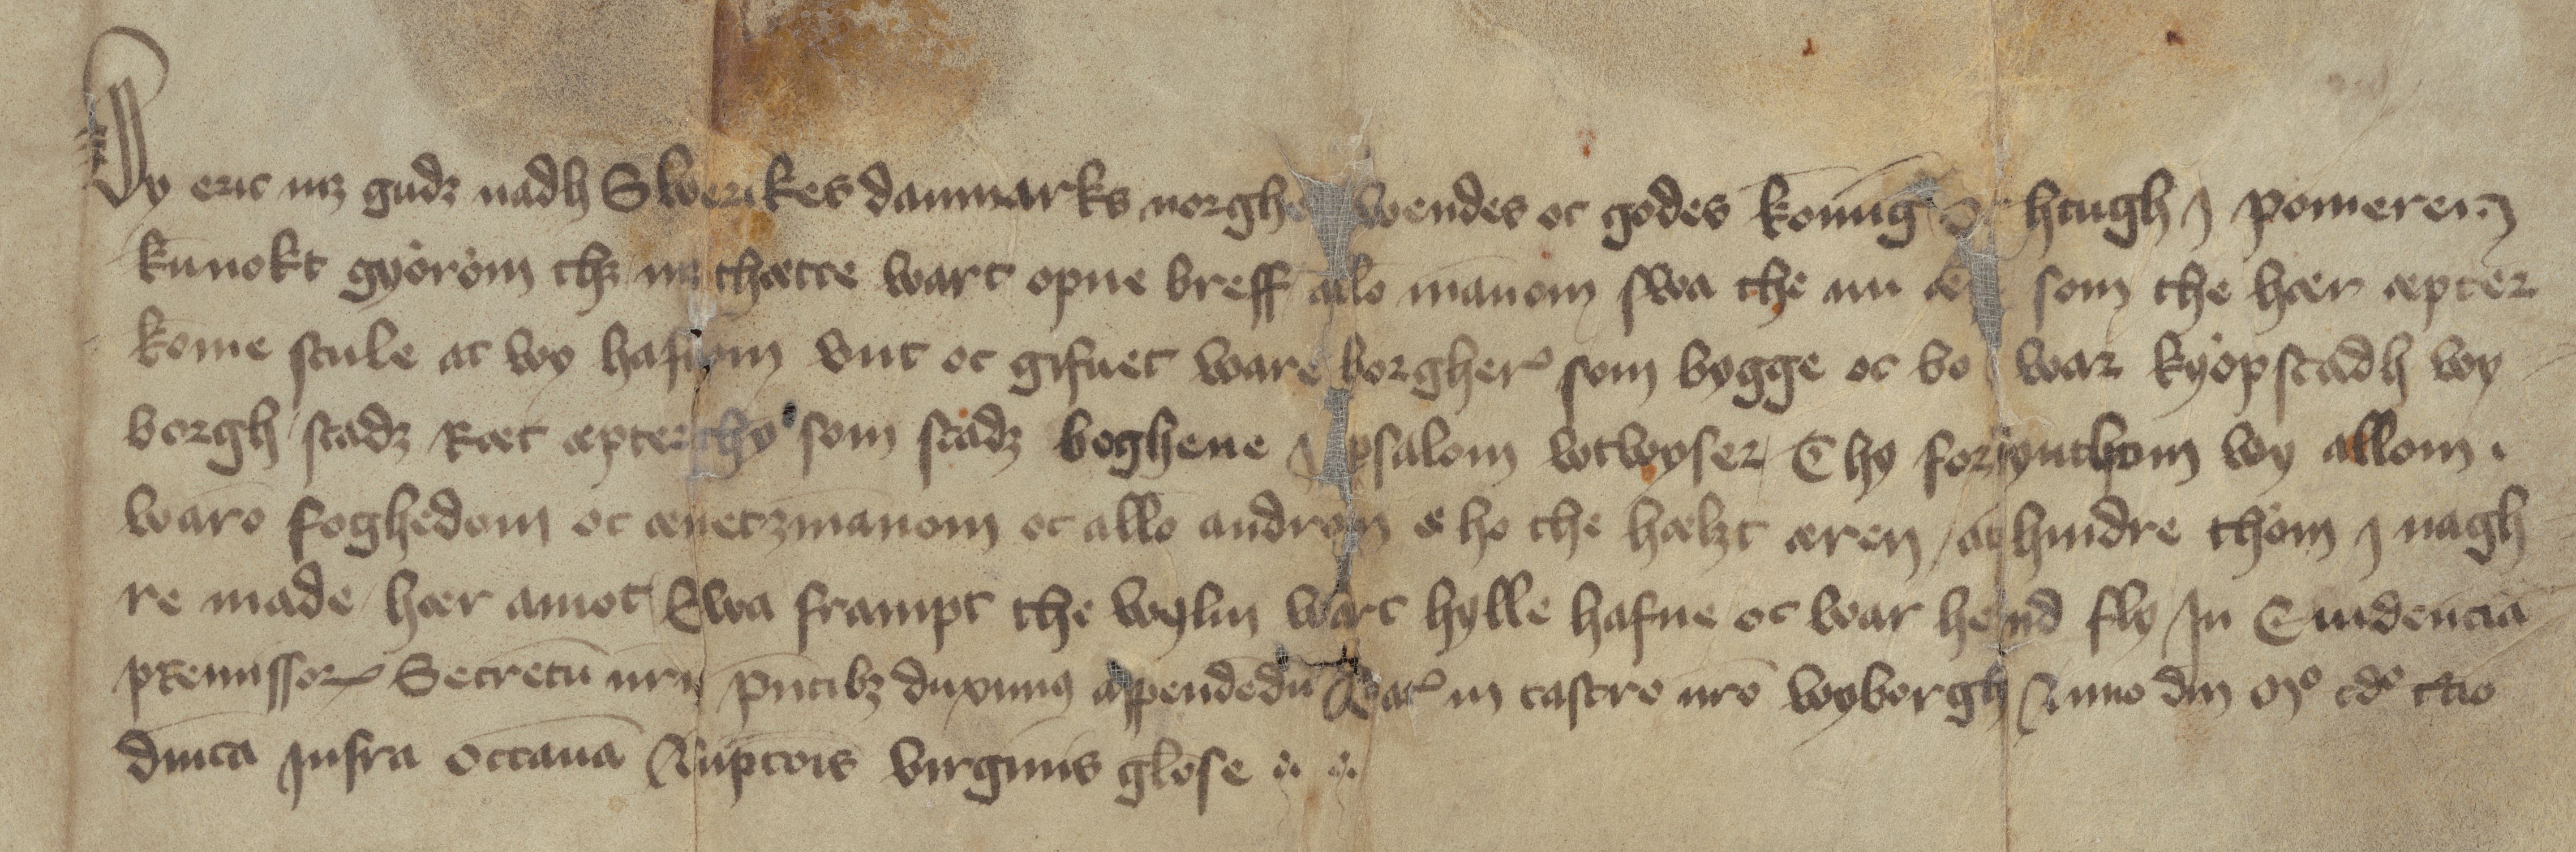
\includegraphics[width=12cm]{pics/viipuri.jpg}      
    \end{center}

    \vspace{1cm}

    { \raggedright\fontsize{16}{16}\fontspec{Aboensis}
      \abcursiveinitial{W}*y eric mz gudz nadh
      Swerikes danmarks norges wendes oc godes konug oc htugh i pomeren
      kunokt györöm thz mz thätte wart opne breff allõ ma~nom swa the nu
      äre som the här äpter kome scule at wy hafvon vnt oc gifuet ware
      borgher som bygge oc bo war kyöpstadh wyborgh, stadz rät äpter
      thy som stadz boghene i upsalom wtwyser, Thy forbythom wy allom.
      warõ foghedom oc änetzma~nom oc allõ androm ä ho the hälzt ären at
      hindre thom i naghre made, här amot, swa frampt the wyliu wart
      hylle hafue oc war hefnd fly In Euidenciã premisso[rum]
      Secret~u nr~m presenti[bus] duxim[us] appended~u
      Datre in castro nrõ wyborgh Anno      dm 
      m`o cd`o  'ttia, dmca infra octauã
      Ass~upcionis virginis 
      glõse ( \ ( }  
    \caption{Charter of the town of Vyborg, \emph{DF 1173, SDHK 16161,
      Kansallisarkisto, Pergamentti-kokoelma, Viipuri 1403-1403}.}
    \label{fig_vyborg}
  \end{figure}
\end{landscape}

%{w}{96}{10mm}{0pt}}\kern-3mm




\subsection{Privilege letter of Olof Nilsson Tawast}


In addition to the account book of Olof Nilsson Tawast
(example \ref{sec_tavast} also one privilege letter of his has
survived. 

A rebellion against King Karl Knutsson broke out in 1457 and he was
forced to take exile in Danzig. Archbishop Jöns Bengtsson
(Oxenstierna) and Erik Axelsson (Tott) were named regents. At that
point Olof Nilsson swapped sides and pledged support to Erik Axelsson.
As a reward Erik extended Olof's noble privileges to several
properties that he had bought from peasants of Tavastia.


\begin{figure}
  \centering
  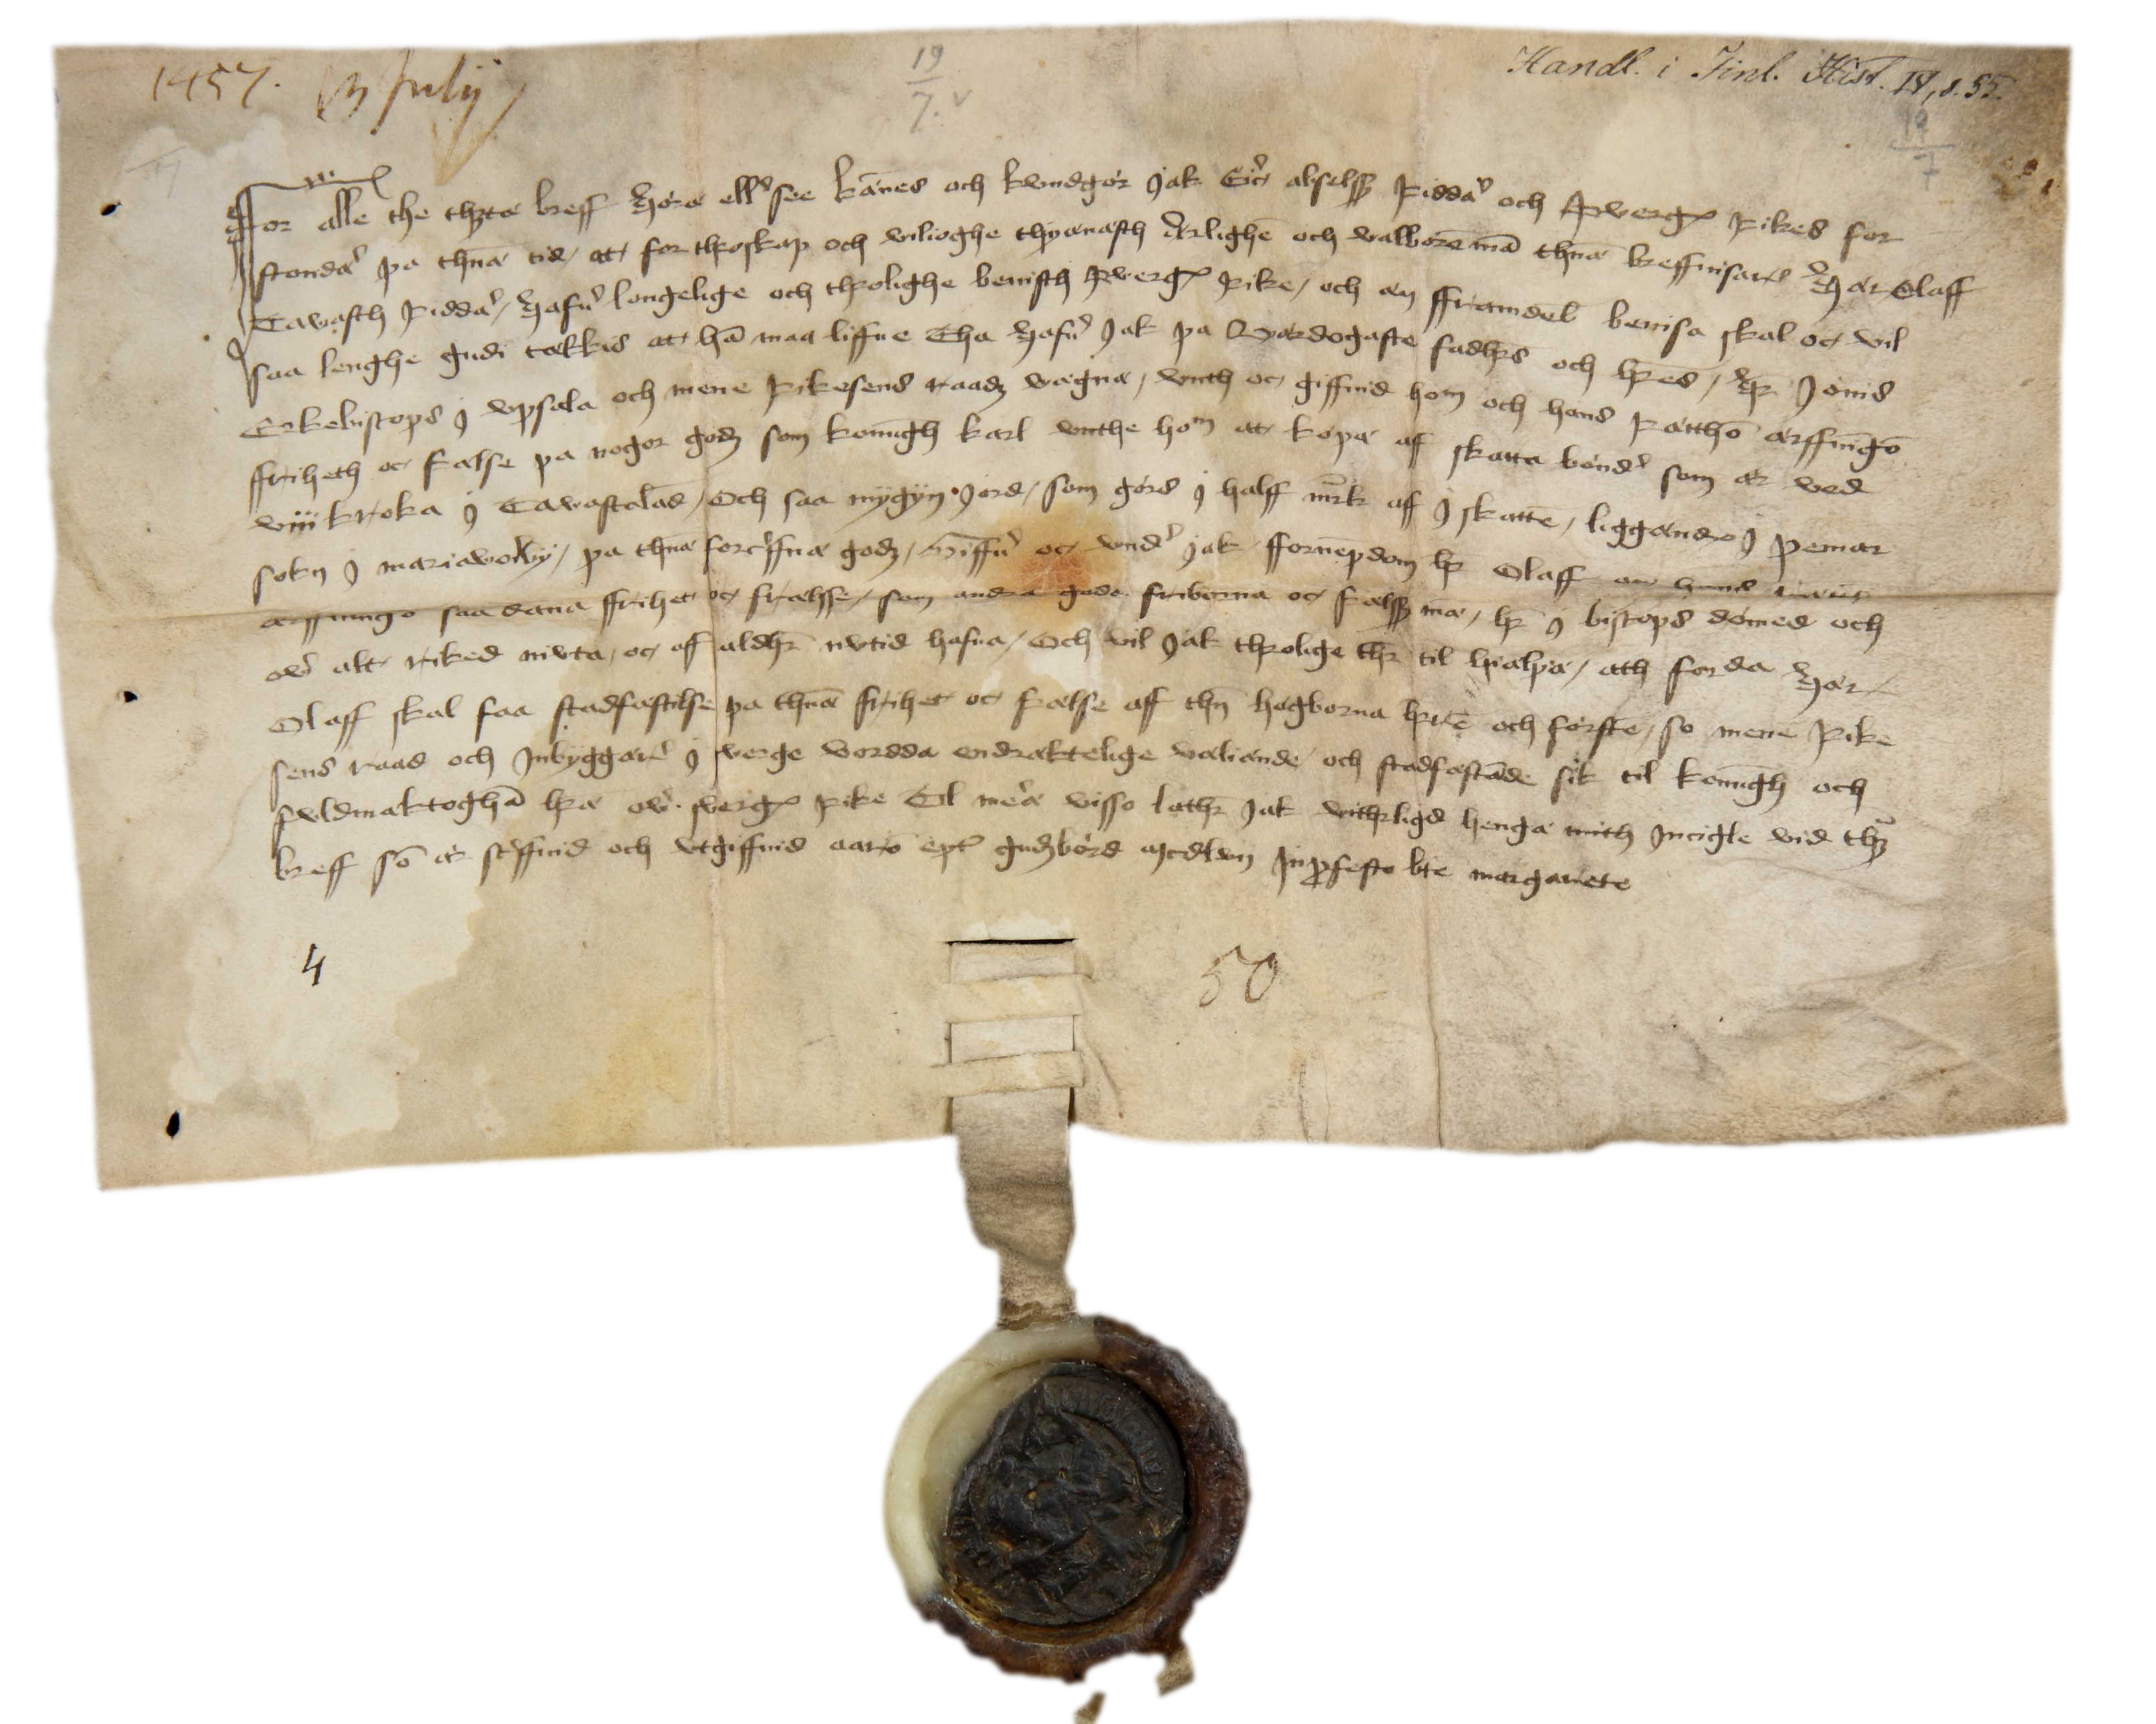
\includegraphics[width=10cm]{pics/SDHK27022.jpg}
  \caption{Privilege letter of Olof Tawast 1457. \emph{DF3038, SDHK 27022}}
  \label{fig_tavast_image}
\end{figure}


\begin{quote}
  For alle the thettæ breff höræ eller see kænnes och kvndgör jak Eric
  Akselsson, riddare och Sverges rikes forstondare pa thennæ tid, at
  for throskap och wilioghe thyænæsth ærlighen och wælboren man thennæ
  breffuisare hær Olaff Tawasth, riddare, hafuer longelige och
  throlighe beuisth Swerges rike och æn fframdelis beuisa skal oc vil
  saa lenghe Gudi tekkis at han maa liffue, tha hafuer jak pa
  wærdogaste fadhers och herres her Jönis, erkebiscops j Vpsala, och
  mene rikesens raadz wægnæ vnth oc giffuid honom och hans rætthom
  ærffuingom ffriheth oc frælse pa nogor godz, som konungh Karl vnthe
  honom at köpæ aff skatta bönder, som ær ved viij kroka j
  Tawastaland, och saa mygyn jord, som görs j halff mark aff j
  skatten, liggændis j Pemar sokn j Mariaworeby. Pa thennæ forscriffnæ
  godz giffuer oc wnder jak fornempdom her Olaff oc hans rættho
  ærffuingo saa dana ffrihet oc frælsse, som andra goda friborna oc
  frælssis mæn her j biscops dömed och ower alt riked nivta oc aff
  aldher nvtid hafua, och vil jak throlige ther til hiælpæ, ath for:da
  hær Olaff skal faa stadfæstilse pa thennæ frihet oc frælse aff then
  högborna herren och försten, som mene rikesens raad och jnbyggære j
  Swerge vordda endræktelige væliænde och stadfæstænde sik til konungh
  och fvldmæktoghan herræ over Sverigis rike. Til meræ visso lather
  jak witherligd hengæ mith jncigle vid thetta breff, som ær scriffuid
  oc vtgiffuid aarom epter Gudz börd mcdlvij jn profesto beate
  Margarete.
\end{quote}


\begin{quote}
  To all who hear or see this letter I, Eric Akselsson, knight and at
  the time regent of the Swedish Realm, tell and make known that for
  loyalty and willing service that the beloved and high-born man, the
  recipient of this letter, Sir Olaff Tawast, knight, has long shown
  to the Swedish realm and will continue to show for so long as God
  wills him live, have I with the worthy Father and Lord, Sir Jöns,
  Archbishop of Uppsala, and the advice of the Council of the Realm
  given him and his lawful heirs freedom and privileges for several
  farmsteads that King Karl let him to buy from tax farmers that make
  8 ploughs in Tavastia and to so much land that pays a half mark in
  taxes that is in Mariavuori village in the Paimio parish. For these
  named farmsteads I give the named Sir Olaff and his lawful heirs
  those freedoms and privileges that other good freeborn and
  privileged men here in bishop's diocese and all over the realm have
  and have always enjoyed, and I will truthfully help to ensure that
  Sir Olaf shall recive these freedoms and privileges when the
  high-born men and lords as the Council of the Realm and the
  inhabitants of Sweden elect and set the King and allmigthy Lord of
  the Swedish Realm. For further proof I will attach my seal to
  this letter that is written and given in Year of the Lord mcdlvii on
  the Feast of St Margarete.
  

\end{quote}




\begin{landscape}
  \begin{figure}
    
    {\fontsize{15}{19}\fontspec{Aboensis}\raggedright
      \abl{\abcursiveinitial{F}or alle the [thet]tä breff hörä
        eller see käñes och kvndgör jak Ei`rc akselss riddare och
        sver[ges] rikes}
      \abl{forstondare pa theñä tid, at for throskap och
      wilioghe thyänästh Ärlighẽ och wälborẽ mã theñä }
    \abl{breffuisare här  Olaff Tawasth, riddare, hafuer longelige och throlighe beuisth
      swer[ges] rike, och}
    \abl{än fframdel[is] beuisa skal oc vil saa
      lenghe gudi täkkis att hã maa liffue, tha hafuer jak pa
      }
    \abl{wärdogaste fadhers och herres, h~r: Jönis, erkebiscops j vpsala
      och mene rikesens raadz wägnä, }
    \abl{ vnth oc giffuid ho`m och hans  rätthõ ärffuingõ ffriheth oc frälse pa nogor godz, som konũgh
       }
    \abl{karl vnthe ho`m at köpä aff skatta bönder som är ved viii kroka
      j Tawastalãd, Och saa mygyn }
    \abl{jord, som görs j halff \abmark{} aff
      j skattẽ, liggändis j Pemar sokn j mariaworeby, pa
      theñä for}
    \abl{scriffnä godz, giffuer oc wnder jak, ffornẽpdom h~r Olaff oc hans rättho ärffuingo saa dana}
    \abl{ffrihet oc frälsse, som andra goda friborna oc frälss m~ä, h~r: j biscops dömed och ower
      alt riked}
    \abl{nivta oc aff aldh~r: nvtid hafua, Och vil jak throlige
      th~r: til hiälpä, ath forda här Olaff skal faa }
    \abl{stadfästilse pa
      theñä frihet oc frälse aff thñ högborna herrẽ och förstẽ, sõ
      mene rikesens raad}
    \abl{och jnbyggäre j swerge vordda endräktelige väliände, och stadfäst~äde sik til konũgh
      och fvldmäk-}
    \abl{toghã h~r:ä over sveri[ges] rike. Til merä visso lath~r: jak witherligd hengä mith jncigle
      vid thetta }
    \abl{breff, sõ är scriffuid oc vtgiffuid aarõ epter gudzbörd mcdlvii jn [pro]festo btẽ margarete. }}
    \caption{Privilege letter of Olof Tawast 1457. \emph{DF3080, SDHK 27022}}
    \label{fig_tavast_privileges}
  \end{figure}
\end{landscape}


\subsection{Bishop Magnus Olai Tawast's admonition}

The copy book of Bishop Magnus Olai Tawast (c. 1370-1452) has
survived. Sometime circa 1430 he reissued an order that a previous
Bishop of Abo, Blessed Hemming had issued 80 years earlier that
prohibited priests to keep their children in their households or to
permit them reside on vicarages. This order was later copied into the
personal copy book of Bishop Magnus Nicolai Särkilahti.

\begin{figure}
  \centering
  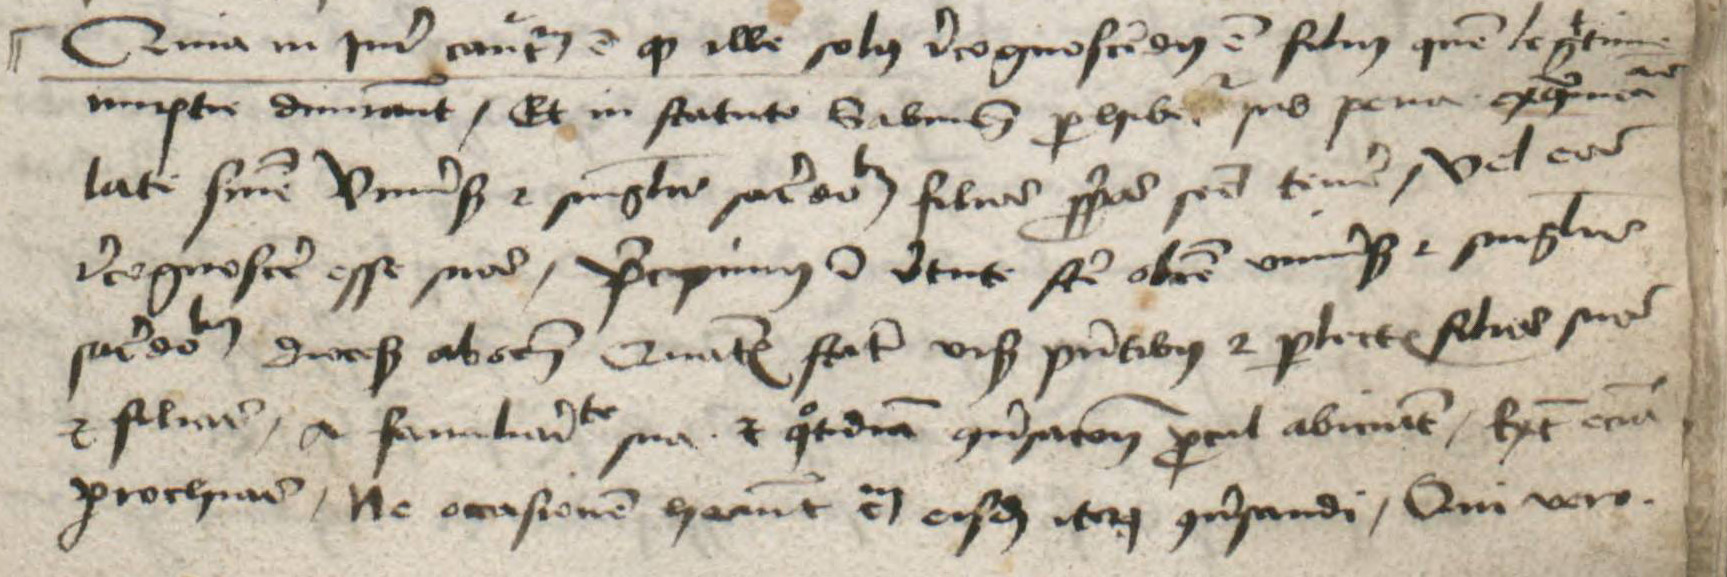
\includegraphics[width=10cm]{pics/DF1423.jpg}
  \caption{Bishop Magnus Olai Tawast's admonition \emph{DF1423}}\label{fig_admonition}
\end{figure}


\begin{figure}
  {\fontsize{15}{20}\fontspec{Aboensis}\raggedright

    \abl{Quia in jure caut`m ẽ [quod] ille
      solus [re]cognoscẽedus}
        \abl{ẽ filius quẽ nupcie
      demõstrant, Et in statutis} 
    \abl{Sabinensi[bus]
      [pro]hibe`t sub pena exco~unicacio~n late}
    \abl{vni[uer] \& sing~lis sac[re]do[bus] filios
      [~prop]as secum tenere}
    \abl{vel eos
      [re]cognoscere esse suos, [pre]cipimus ~i
      [ver]tute  st~e}
    \abl{ob~e~e vni[ver]ss \& singulis
      sac[er]do`[bus] diocss aboe~s Quat~e}
    \abl{stat~i viss
      p~rtibus \& [per]lect~i, filios suos \& filias, a fam}
    \abl{mili~r`t`e sua \& [quo]tdnã
      [con][ver]sacione [pro]cul abicia~t, eciã extra}
    \abl{[par]rochias, ne occasione~m habea~t c`m
      eis ite[rum] [con]~usandi}}
  \caption{Beginning of Blessed Hemming's order to priest as given in
    Magnus Nicolai's copybook (DF 1423, DF 563)}
  \label{fig_hemming}
\end{figure}


\begin{quote}
  Quia jn iure cautum est, quod ille solus recognoscendus est filius,
  quem nupcie demonstrant, et in statutis Sabinensibus prohibetur sub
  pena excommunicacionis late vniuersis et singulis sacerdotibus
  filios proprios secum tenere uel eos recognoscere esse suos,
  precipimus in virtute sancte obediencie vniuersis et singulis
  sacerdotibus dyocesis Aboensis, quatenus statim, visis presentibus
  et perlectis, filios suos et filias a familiaritate sua et cotidiana
  conuersacione procul abiciant, eciam extra parrochias, ne occasionem
  habeant cum eis iterum conuersandj. 
\end{quote}



\newpage


\subsection{Cursive initials in The Black Book}\label{ssec_black_book}

This section shows a bit of the context for the cursive initials that
were taken from \emph{The Black Book of Åbo Cathedral} to show how
they were positioned among the text. The \emph{Y} is not actually a
initial, but it was the only capital \emph{Y} that I could find from
the book. 

\label{cursive_start}
\begin{longtable}{ccc}
  
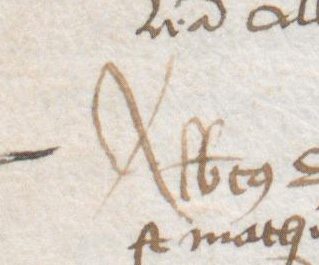
\includegraphics[width=3.5cm]{pics/rea-A.jpg} &
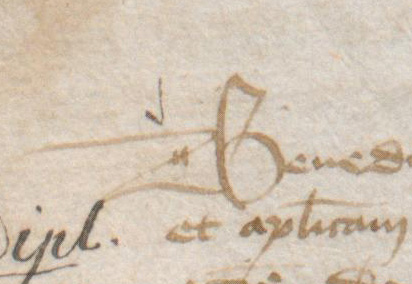
\includegraphics[width=3.5cm]{pics/rea-B.jpg} &
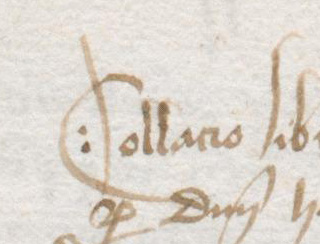
\includegraphics[width=3.5cm]{pics/rea-C.jpg} \\

A & B & C \\

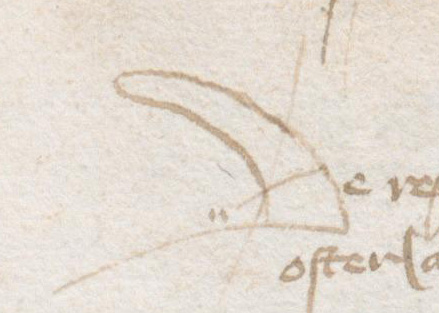
\includegraphics[width=3.5cm]{pics/rea-D.jpg} &
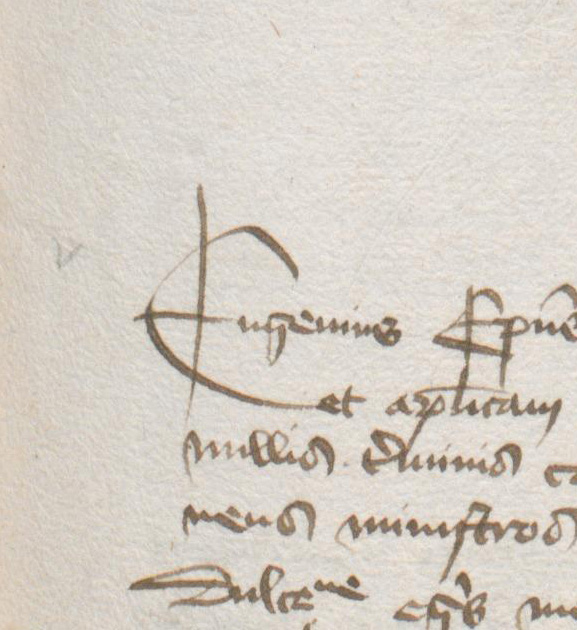
\includegraphics[width=3.5cm]{pics/rea-E.jpg} &
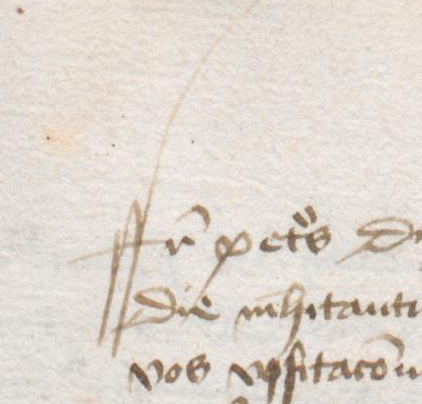
\includegraphics[width=3.5cm]{pics/rea-F.jpg} \\

D & E & F \\

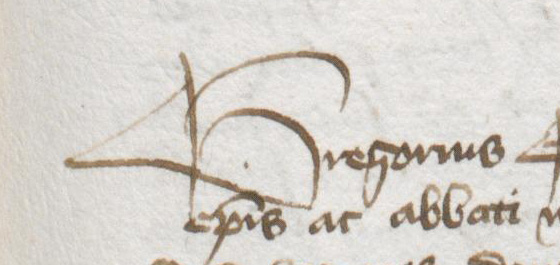
\includegraphics[width=3.5cm]{pics/rea-G.jpg} &
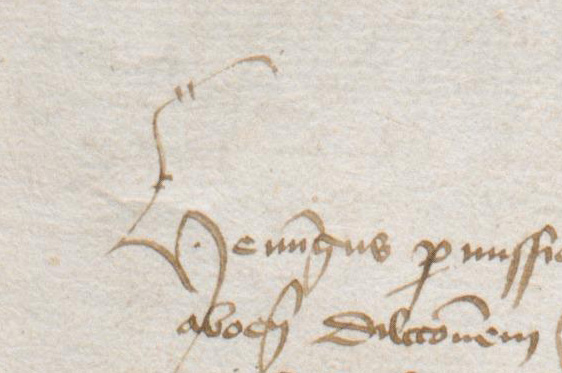
\includegraphics[width=3.5cm]{pics/rea-H.jpg} &
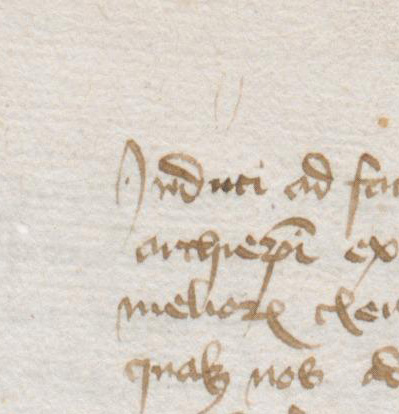
\includegraphics[width=3.5cm]{pics/rea-I.jpg} \\

G & H & I \\

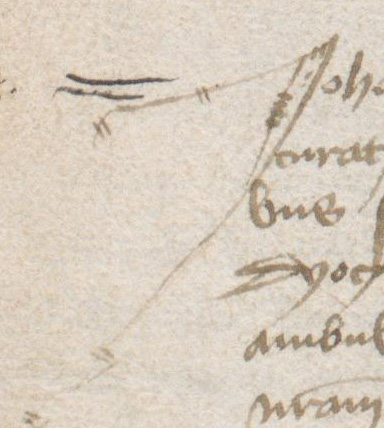
\includegraphics[width=3.5cm]{pics/rea-J.jpg} &
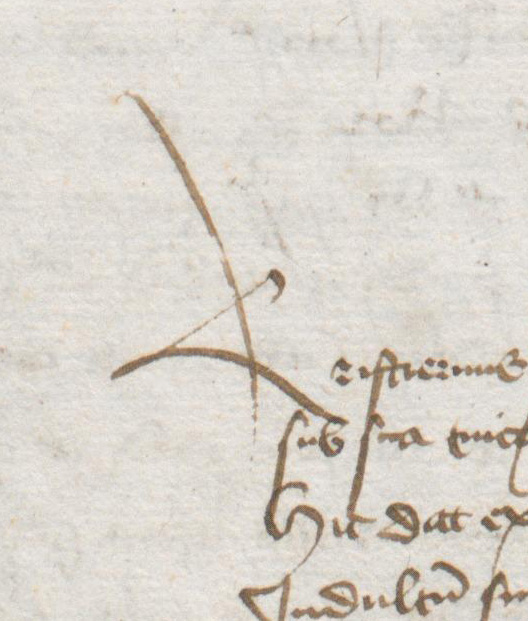
\includegraphics[width=3.5cm]{pics/rea-K.jpg} &
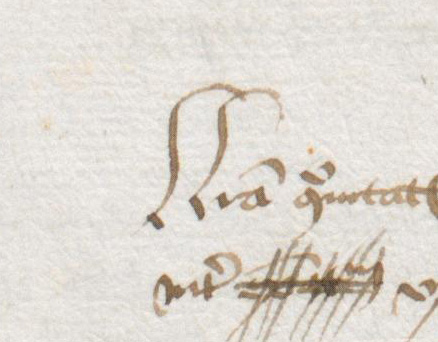
\includegraphics[width=3.5cm]{pics/rea-L.jpg} \\

J & K & L \\

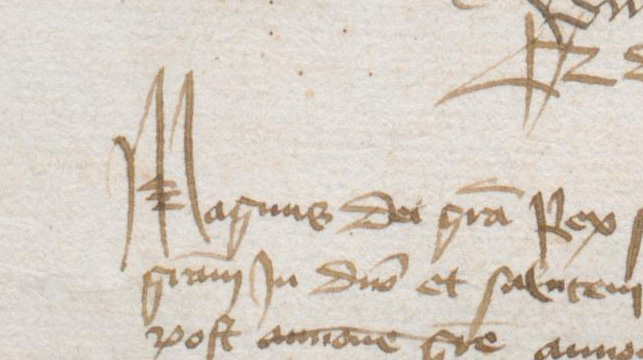
\includegraphics[width=3.5cm]{pics/rea-M.jpg} &
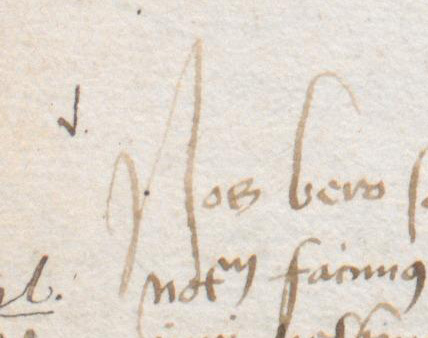
\includegraphics[width=3.5cm]{pics/rea-N.jpg} &
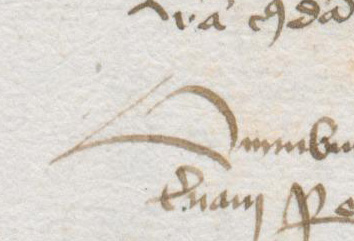
\includegraphics[width=3.5cm]{pics/rea-O.jpg} \\

M & N & O \\

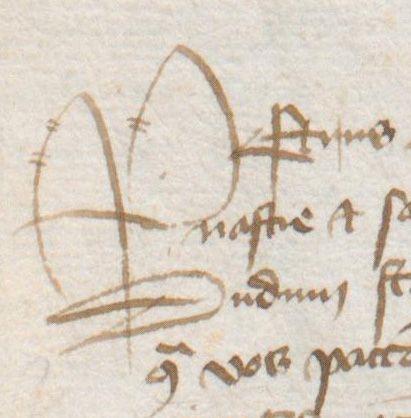
\includegraphics[width=3.5cm]{pics/rea-P.jpg} &
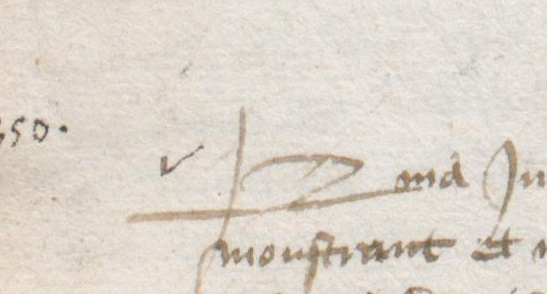
\includegraphics[width=3.5cm]{pics/rea-Q.jpg} &
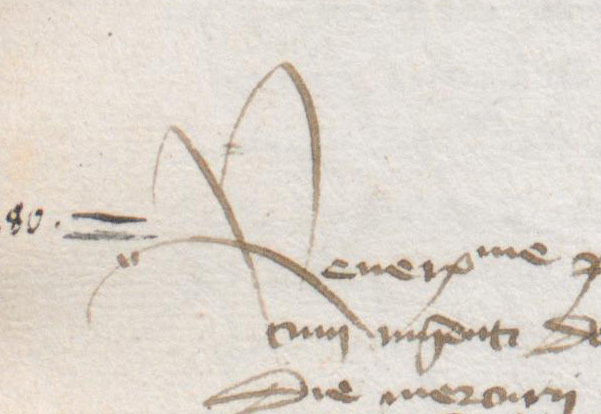
\includegraphics[width=3.5cm]{pics/rea-R.jpg} \\

P & Q & R \\

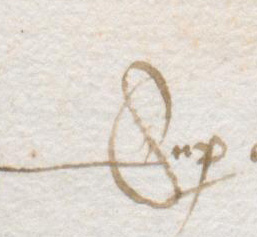
\includegraphics[width=3.5cm]{pics/rea-S.jpg} &
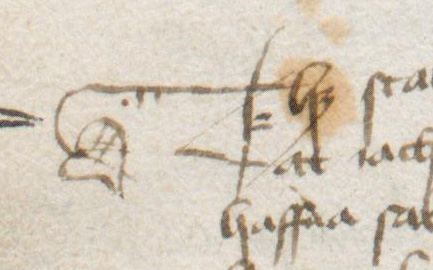
\includegraphics[width=3.5cm]{pics/rea-T.jpg} &
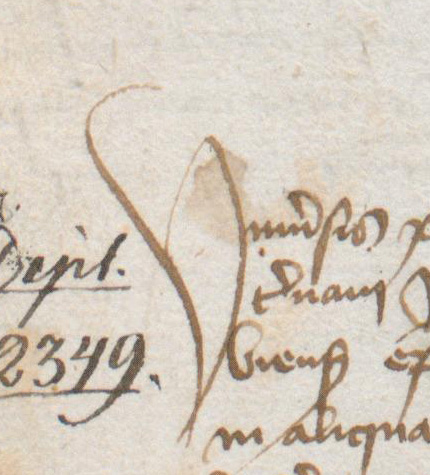
\includegraphics[width=3.5cm]{pics/rea-U.jpg} \\

S & T & U \\

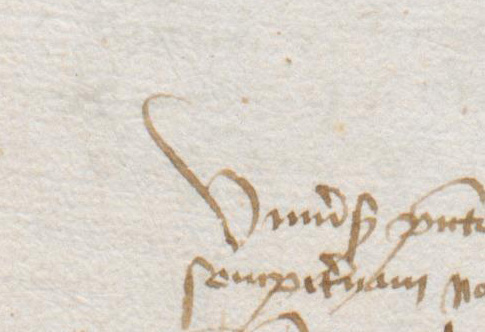
\includegraphics[width=3.5cm]{pics/rea-V.jpg} &
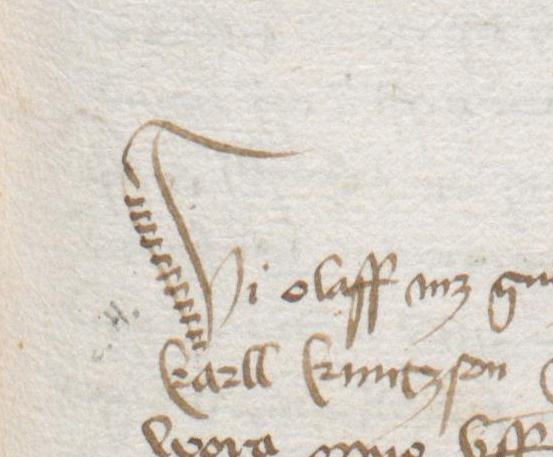
\includegraphics[width=3.5cm]{pics/rea-W.jpg} &
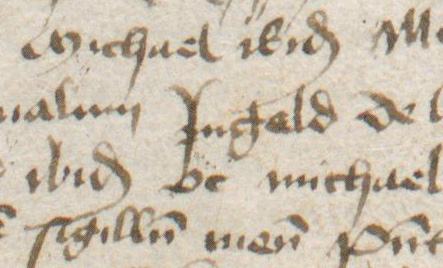
\includegraphics[width=3.5cm]{pics/rea-Y.jpg} \\

W & W & Y \\

\end{longtable}
\label{cursive_end}


\section{List of Symbols}

\label{pg:symbols_start}

\newcommand{\absymbolsample}[2]{\showlettertitle{#1}{#2}}
\newcommand{\absymbolsampletwo}[2]{\showlettertitletwo{#1}{#2}}




\newcommand{\abhd}[1]{\multicolumn{4}{l}{\textbf{#1}}\\}

\begin{longtable}{l@{ }l@{ }l@{ }l@{ }l@{ }l@{ }l@{}@{ }l@{}@{ }l@{ }l@{ }l}

\abhd{A}

\absymbolsample{\char`\^^^^0041}{0041} & 
\absymbolsample{\char`\^^^^00c4}{00c4} &
\absymbolsample{\char`\^^^^00c5}{00c5} &
\absymbolsample{\char`\^^^^0061}{0061} & 
 \absymbolsample{\char`\^^^^f514}{f514} & 
\absymbolsample{\char`\^^^^00e1}{00e1} & 
\absymbolsample{\char`\^^^^f570}{f570} & 
\absymbolsample{\char`\^^^^00e4}{00e4} & 
\absymbolsample{\char`\^^^^f569}{f569} & 
\absymbolsample{\char`\^^^^00e5}{00e5} &
 \absymbolsample{\char`\^^^^f568}{f568} \\

\absymbolsample{\char`\^^^^00e3}{00e3} &
\absymbolsample{\char`\^^^^f4b2}{f4b2} & 
\absymbolsample{\char`\^^^^f52c}{f52c} & 
 \absymbolsample{\char`\^^^^f496}{f496} & 
\absymbolsample{\char`\^^^^f574}{f574} & 

\absymbolsample{\char`\^^^^00e6}{00e6} & 
\absymbolsample{\char`\^^^^f41d}{f41d} &
 \absymbolsample{\char`\^^^^f43a}{f43a} &
\absymbolsample{\char`\^^^^f400}{f400} &
\absymbolsample{\char`\^^^^f41e}{f41e} &
 \absymbolsample{\char`\^^^^f43b}{f43b} \\   
\absymbolsample{\char`\^^^^f401}{f401} & 
\absymbolsample{\char`\^^^^f41f}{f41f} & 
 \absymbolsample{\char`\^^^^f43c}{f43c} & 
\absymbolsample{\char`\^^^^f402}{f402} & 

 \absymbolsample{\char`\^^^^f476}{f476} & 
 \absymbolsample{\char`\^^^^f458}{f458} & 

 \absymbolsample{\char`\^^^^f477}{f477} & 
 \absymbolsample{\char`\^^^^f459}{f459} &

 \absymbolsample{\char`\^^^^f478}{f478} & 
 \absymbolsample{\char`\^^^^f45a}{f45a} & 




 \absymbolsample{\char`\^^^^f52e}{f52e} \\
 \absymbolsample{\char`\^^^^f52f}{f52f} &
 \absymbolsample{\char`\^^^^f530}{f530} & 
\absymbolsample{\char`\^^^^f579}{f579} & 
 \absymbolsample{\char`\^^^^f54e}{f54e} &




\\\abhd{B}

 \absymbolsample{\char`\^^^^0042}{0042}&
 \absymbolsample{\char`\^^^^0062}{0062} & 
\absymbolsample{\char`\^^^^f420}{f420} & 
 \absymbolsample{\char`\^^^^f43d}{f43d} & 
 \absymbolsample{\char`\^^^^f403}{f403} & 
 \absymbolsample{\char`\^^^^f479}{f479} & 
 \absymbolsample{\char`\^^^^f45b}{f45b} & 
 \absymbolsample{\char`\^^^^f531}{f531} & 
 \absymbolsample{\char`\^^^^f54f}{f54f} & 
 \absymbolsample{\char`\^^^^f5e3}{f5e3} & 

\\\abhd{C}

 \absymbolsample{\char`\^^^^0043}{0043}&
 \absymbolsample{\char`\^^^^0063}{0063} &  
 \absymbolsample{\char`\^^^^0107}{0107} & 
 \absymbolsample{\char`\^^^^f4b6}{f4b6} & 
\absymbolsample{\char`\^^^^f421}{f421} & 
 \absymbolsample{\char`\^^^^f43e}{f43e} & 
 \absymbolsample{\char`\^^^^f404}{f404} & 
 \absymbolsample{\char`\^^^^f47a}{f47a} & 
 \absymbolsample{\char`\^^^^f45c}{f45c} & 
 \absymbolsample{\char`\^^^^f532}{f532} & 
 \absymbolsample{\char`\^^^^f550}{f550} \\
 \absymbolsample{\char`\^^^^f583}{f583} & 
 \absymbolsample{\char`\^^^^f584}{f584} & 
 \absymbolsample{\char`\^^^^f5f5}{f5f5} & 

\\\abhd{D}

 \absymbolsample{\char`\^^^^0044}{0044}&
 \absymbolsample{\char`\^^^^f457}{f457} & 
 \absymbolsample{\char`\^^^^0064}{0064} & 
 \absymbolsample{\char`\^^^^f4b7}{f4b7} &
 \absymbolsample{\char`\^^^^f519}{f519} & 
 \absymbolsample{\char`\^^^^f54d}{f54d} & 
\absymbolsample{\char`\^^^^f422}{f422} &  
 \absymbolsample{\char`\^^^^f43f}{f43f} & 
 \absymbolsample{\char`\^^^^f405}{f405} & 

 \absymbolsample{\char`\^^^^f47b}{f47b} & 
 \absymbolsample{\char`\^^^^f45d}{f45d} \\

 \absymbolsample{\char`\^^^^f493}{f493} & 
 \absymbolsample{\char`\^^^^f475}{f475} & 
 \absymbolsample{\char`\^^^^f533}{f533} & 
 \absymbolsample{\char`\^^^^f586}{f586} & 
 \absymbolsample{\char`\^^^^f551}{f551} & 
\absymbolsample{\char`\^^^^f578}{f578} & 
\absymbolsample{\char`\^^^^f5ef}{f5ef} & 
\absymbolsample{\char`\^^^^f5f0}{f5f0} & 
\absymbolsample{\char`\^^^^f5f1}{f5f1} & 
\absymbolsample{\char`\^^^^f5f2}{f5f2} & 


\\\abhd{E}

\absymbolsample{\char`\^^^^0045}{0045}  &
 \absymbolsample{\char`\^^^^0065}{0065} & 
 \absymbolsample{\char`\^^^^f4b3}{f4b3} & 
 \absymbolsample{\char`\^^^^f497}{f497} &
 \absymbolsample{\char`\^^^^00e9}{00e9} & 
\absymbolsample{\char`\^^^^f571}{f571} & 
 \absymbolsample{\char`\^^^^00eb}{00eb} & 
 \absymbolsample{\char`\^^^^1ebd}{1ebd} &
 \absymbolsample{\char`\^^^^f4b4}{f4b4} & 
 \absymbolsample{\char`\^^^^f498}{f498} & 
 \absymbolsample{\char`\^^^^f4d1}{f4d1} \\
 \absymbolsample{\char`\^^^^f58b}{f58b} & 
 \absymbolsample{\char`\^^^^f4d2}{f4d2} & 
\absymbolsample{\char`\^^^^f423}{f423} &  
 \absymbolsample{\char`\^^^^f440}{f440} & 
 \absymbolsample{\char`\^^^^f406}{f406} & 
 \absymbolsample{\char`\^^^^f47c}{f47c} & 
 \absymbolsample{\char`\^^^^f45e}{f45e} & 
 \absymbolsample{\char`\^^^^f534}{f534} & 
 \absymbolsample{\char`\^^^^f552}{f552} & 
 \absymbolsample{\char`\^^^^f5e5}{f5e5} & 



\\\abhd{F}

\absymbolsample{\char`\^^^^0046}{0046}  &
 \absymbolsample{\char`\^^^^0066}{0066} &
\absymbolsample{\char`\^^^^f424}{f424} & 
 \absymbolsample{\char`\^^^^f441}{f441} & 
\absymbolsample{\char`\^^^^f407}{f407} & 
 \absymbolsample{\char`\^^^^f47d}{f47d} & 
 \absymbolsample{\char`\^^^^f45f}{f45f} & 
 \absymbolsample{\char`\^^^^f535}{f535} & 
 \absymbolsample{\char`\^^^^f553}{f553} & 

\\\abhd{G}

\absymbolsample{\char`\^^^^0047}{0047}  &
 \absymbolsample{\char`\^^^^0067}{0067} & 
 \absymbolsample{\char`\^^^^f4ad}{f4ad} & 
 \absymbolsample{\char`\^^^^01f5}{01f5} & 
 \absymbolsample{\char`\^^^^f4bb}{f4bb} & 
 \absymbolsample{\char`\^^^^f4c5}{f4c5} &
\absymbolsample{\char`\^^^^f425}{f425} & 
 \absymbolsample{\char`\^^^^f442}{f442} & 
 \absymbolsample{\char`\^^^^f408}{f408} & 
 \absymbolsample{\char`\^^^^f47e}{f47e} & 
 \absymbolsample{\char`\^^^^f460}{f460} \\
 \absymbolsample{\char`\^^^^f536}{f536} & 
 \absymbolsample{\char`\^^^^f554}{f554} & 
 \absymbolsample{\char`\^^^^f589}{f589} & 
 \absymbolsample{\char`\^^^^f58a}{f58a} & 
 \absymbolsample{\char`\^^^^f5e6}{f5e6} & 


\\\abhd{H}

\absymbolsample{\char`\^^^^0048}{0048}  &
\absymbolsample{\char`\^^^^0068}{0068} & 
 \absymbolsample{\char`\^^^^f555}{f555} & 
\absymbolsample{\char`\^^^^f56a}{f56a} &
 \absymbolsample{\char`\^^^^f5ca}{f5ca} & 
\absymbolsample{\char`\^^^^f426}{f426} & 
 \absymbolsample{\char`\^^^^f443}{f443} & 
\absymbolsample{\char`\^^^^f409}{f409} & 
 \absymbolsample{\char`\^^^^f47f}{f47f} & 
 \absymbolsample{\char`\^^^^f461}{f461} & 
 \absymbolsample{\char`\^^^^f4aa}{f4aa} \\
 \absymbolsample{\char`\^^^^f537}{f537} & 


\\\abhd{I}

\absymbolsample{\char`\^^^^0049}{0049}  &
\absymbolsample{\char`\^^^^0069}{0069} & 
 \absymbolsample{\char`\^^^^f495}{f495} & 
\absymbolsample{\char`\^^^^00ed}{00ed} & 
\absymbolsample{\char`\^^^^0129}{0129} & 
 \absymbolsample{\char`\^^^^f4b8}{f4b8} & 
 \absymbolsample{\char`\^^^^f49a}{f49a} &
\absymbolsample{\char`\^^^^f427}{f427} & 
 \absymbolsample{\char`\^^^^f444}{f444} & 
\absymbolsample{\char`\^^^^f40a}{f40a} & 
 \absymbolsample{\char`\^^^^f480}{f480} \\ 
 \absymbolsample{\char`\^^^^f462}{f462} & 


 \absymbolsample{\char`\^^^^f538}{f538} & 
 \absymbolsample{\char`\^^^^f557}{f557} & 


\\\abhd{J}

\absymbolsample{\char`\^^^^004a}{004a}  &
\absymbolsample{\char`\^^^^006a}{006a} & 
 \absymbolsample{\char`\^^^^f499}{f499} & 
 \absymbolsample{\char`\^^^^f49f}{f49f} & 
 \absymbolsample{\char`\^^^^f521}{f521} & 
 \absymbolsample{\char`\^^^^f51a}{f51a} & 
 \absymbolsample{\char`\^^^^f4bf}{f4bf} & 
 \absymbolsample{\char`\^^^^f5cc}{f5cc} & 
\absymbolsample{\char`\^^^^f428}{f428} & 
 \absymbolsample{\char`\^^^^f445}{f445} & 
\absymbolsample{\char`\^^^^f40b}{f40b} \\
 \absymbolsample{\char`\^^^^f481}{f481} & 
 \absymbolsample{\char`\^^^^f463}{f463} & 
 \absymbolsample{\char`\^^^^f539}{f539} & 
 \absymbolsample{\char`\^^^^f5ce}{f5ce} & 

\\\abhd{K}


\absymbolsample{\char`\^^^^004b}{004b}  &
\absymbolsample{\char`\^^^^006b}{006b} & 
 \absymbolsample{\char`\^^^^f4a0}{f4a0} & 
\absymbolsample{\char`\^^^^f56b}{f56b} & 
 \absymbolsample{\char`\^^^^f522}{f522} & 
\absymbolsample{\char`\^^^^f429}{f429} & 
 \absymbolsample{\char`\^^^^f446}{f446} & 
\absymbolsample{\char`\^^^^f40c}{f40c} & 
 \absymbolsample{\char`\^^^^f482}{f482} & 
 \absymbolsample{\char`\^^^^f464}{f464} & 
 \absymbolsample{\char`\^^^^f53a}{f53a} \\
 \absymbolsample{\char`\^^^^f558}{f558} &
 \absymbolsample{\char`\^^^^f58e}{f58e} & 

\\\abhd{L}

 \absymbolsample{\char`\^^^^004c}{004c}  &
\absymbolsample{\char`\^^^^006c}{006c} & 
 \absymbolsample{\char`\^^^^f4ab}{f4ab} & 
 \absymbolsample{\char`\^^^^f4c0}{f4c0} & 
 \absymbolsample{\char`\^^^^f572}{f572} & 
 \absymbolsample{\char`\^^^^f5c8}{f5c8} & 
\absymbolsample{\char`\^^^^f42a}{f42a} & 
 \absymbolsample{\char`\^^^^f447}{f447} & 
\absymbolsample{\char`\^^^^f40d}{f40d} & 
 \absymbolsample{\char`\^^^^f483}{f483} & 
 \absymbolsample{\char`\^^^^f465}{f465} \\
 \absymbolsample{\char`\^^^^f53b}{f53b} & 
 \absymbolsample{\char`\^^^^f559}{f559} &

\\\abhd{M}

\absymbolsample{\char`\^^^^004d}{004d} & 
\absymbolsample{\char`\^^^^006d}{006d} & 
\absymbolsample{\char`\^^^^f4a1}{f4a1} & 
\absymbolsample{\char`\^^^^f49b}{f49b} & 
 \absymbolsample{\char`\^^^^f4a7}{f4a7} &
\absymbolsample{\char`\^^^^f4c1}{f4c1} & 
 \absymbolsample{\char`\^^^^f4b9}{f4b9} & 
 \absymbolsample{\char`\^^^^f4bc}{f4bc} & 
 \absymbolsample{\char`\^^^^f515}{f515} & 
\absymbolsample{\char`\^^^^1e3f}{1e3f} & 
 \absymbolsample{\char`\^^^^f51b}{f51b} \\
 \absymbolsample{\char`\^^^^f4e3}{f4e3} & 
 \absymbolsample{\char`\^^^^f513}{f513} & 
\absymbolsample{\char`\^^^^f42b}{f42b} &
 \absymbolsample{\char`\^^^^f448}{f448} & 
\absymbolsample{\char`\^^^^f40e}{f40e} & 
 \absymbolsample{\char`\^^^^f484}{f484} & 
 \absymbolsample{\char`\^^^^f466}{f466} & 
 \absymbolsample{\char`\^^^^f53c}{f53c} & 
 \absymbolsample{\char`\^^^^f55a}{f55a} & 
 \absymbolsample{\char`\^^^^f5e7}{f5e7} & 

\\\abhd{N}

\absymbolsample{\char`\^^^^004e}{004e} & 
\absymbolsample{\char`\^^^^006e}{006e} & 
 \absymbolsample{\char`\^^^^f4a2}{f4a2} & 
 \absymbolsample{\char`\^^^^f49c}{f49c} & 
\absymbolsample{\char`\^^^^f575}{f575} & 
\absymbolsample{\char`\^^^^0144}{0144} & 
 \absymbolsample{\char`\^^^^f51c}{f51c} &
\absymbolsample{\char`\^^^^00f1}{00f1} & 
 \absymbolsample{\char`\^^^^f4ba}{f4ba} & 
\absymbolsample{\char`\^^^^f42c}{f42c} & 
 \absymbolsample{\char`\^^^^f449}{f449} \\
\absymbolsample{\char`\^^^^f40f}{f40f} & 
 \absymbolsample{\char`\^^^^f485}{f485} & 
 \absymbolsample{\char`\^^^^f467}{f467} & 
 \absymbolsample{\char`\^^^^f53d}{f53d} & 
 \absymbolsample{\char`\^^^^f55b}{f55b} & 


\\\abhd{O}

\absymbolsample{\char`\^^^^004f}{004f} & 
\absymbolsample{\char`\^^^^00d6}{00d6} & 
\absymbolsample{\char`\^^^^006f}{006f} & 
\absymbolsample{\char`\^^^^00f6}{00f6} & 
\absymbolsample{\char`\^^^^0153}{0153} & 
 \absymbolsample{\char`\^^^^f52d}{f52d} & 
\absymbolsample{\char`\^^^^00f5}{00f5} & 
\absymbolsample{\char`\^^^^00f3}{00f3} & 
\absymbolsample{\char`\^^^^f42d}{f42d} &
 \absymbolsample{\char`\^^^^f44a}{f44a} & 
\absymbolsample{\char`\^^^^f410}{f410} \\
\absymbolsample{\char`\^^^^f42e}{f42e} &
 \absymbolsample{\char`\^^^^f44b}{f44b} &
\absymbolsample{\char`\^^^^f411}{f411} &
 \absymbolsample{\char`\^^^^f486}{f486} & 
 \absymbolsample{\char`\^^^^f468}{f468} & 
 \absymbolsample{\char`\^^^^f487}{f487} & 
 \absymbolsample{\char`\^^^^f469}{f469} & 
 \absymbolsample{\char`\^^^^f53e}{f53e} & 
 \absymbolsample{\char`\^^^^f53f}{f53f} & 
 \absymbolsample{\char`\^^^^f55c}{f55c} & 
 \absymbolsample{\char`\^^^^f5e2}{f5e2} 


\\\abhd{P}



\absymbolsample{\char`\^^^^0050}{0050} & 
\absymbolsample{\char`\^^^^0070}{0070} & 
 \absymbolsample{\char`\^^^^f4a3}{f4a3} & 

 \absymbolsample{\char`\^^^^f4e4}{f4e4} & 

 \absymbolsample{\char`\^^^^f520}{f520} & 
 \absymbolsample{\char`\^^^^f4e5}{f4e5} &

\absymbolsample{\char`\^^^^f56c}{f56c} & 
 \absymbolsample{\char`\^^^^f4e8}{f4e8} & 


 \absymbolsample{\char`\^^^^f4e7}{f4e7} & 
\absymbolsample{\char`\^^^^1e55}{1e55} & 

\absymbolsample{\char`\^^^^f42f}{f42f} \\
 \absymbolsample{\char`\^^^^f44c}{f44c} &
\absymbolsample{\char`\^^^^f412}{f412} & 
 \absymbolsample{\char`\^^^^f488}{f488} & 
 \absymbolsample{\char`\^^^^f46a}{f46a} & 


 \absymbolsample{\char`\^^^^f540}{f540} & 
 \absymbolsample{\char`\^^^^f55d}{f55d} & 
 \absymbolsample{\char`\^^^^f507}{f507} & 
 \absymbolsample{\char`\^^^^f5df}{f5df} & 
 \absymbolsample{\char`\^^^^f5e0}{f5e0} & 
 \absymbolsample{\char`\^^^^f5e8}{f5e8} & 
 \absymbolsample{\char`\^^^^f5e9}{f5e9} \\
 \absymbolsample{\char`\^^^^f5ea}{f5ea} & 
 \absymbolsample{\char`\^^^^f5eb}{f5eb} & 


\\\abhd{Q}


\absymbolsample{\char`\^^^^0051}{0051} & 
\absymbolsample{\char`\^^^^0071}{0071} & 

 \absymbolsample{\char`\^^^^f4c2}{f4c2} & 
 \absymbolsample{\char`\^^^^f4eb}{f4eb} &
 \absymbolsample{\char`\^^^^f4ec}{f4ec} & 
\absymbolsample{\char`\^^^^f523}{f523} & 
 \absymbolsample{\char`\^^^^f596}{f596} & 
\absymbolsample{\char`\^^^^f430}{f430} & 
 \absymbolsample{\char`\^^^^f44d}{f44d} & 
\absymbolsample{\char`\^^^^f413}{f413} & 
 \absymbolsample{\char`\^^^^f489}{f489} \\
 \absymbolsample{\char`\^^^^f46b}{f46b} & 





 
 \absymbolsample{\char`\^^^^f541}{f541} & 
 \absymbolsample{\char`\^^^^f55e}{f55e} & 
 \absymbolsample{\char`\^^^^f4ed}{f4ed} & 
 \absymbolsample{\char`\^^^^f4e9}{f4e9} & 
 \absymbolsample{\char`\^^^^f4ea}{f4ea} & 
 \absymbolsample{\char`\^^^^f5bd}{f5bd} & 
 \absymbolsample{\char`\^^^^f5e1}{f5e1} & 
 \absymbolsample{\char`\^^^^f5ec}{f5ec} & 


\\\abhd{R}


\absymbolsample{\char`\^^^^0052}{0052} & 
\absymbolsample{\char`\^^^^0072}{0072} & 
 \absymbolsample{\char`\^^^^f4a4}{f4a4} & 
 \absymbolsample{\char`\^^^^f4a8}{f4a8} & 
 \absymbolsample{\char`\^^^^f4b5}{f4b5} &
 \absymbolsample{\char`\^^^^f4c3}{f4c3} & 
 \absymbolsample{\char`\^^^^f4c4}{f4c4} & 
\absymbolsample{\char`\^^^^0155}{0155} & 
\absymbolsample{\char`\^^^^f56f}{f56f} & 
 \absymbolsample{\char`\^^^^f5c9}{f5c9} & 


\absymbolsample{\char`\^^^^f431}{f431} \\
 \absymbolsample{\char`\^^^^f44e}{f44e} &
\absymbolsample{\char`\^^^^f414}{f414} & 
 \absymbolsample{\char`\^^^^f48a}{f48a} & 
 \absymbolsample{\char`\^^^^f46c}{f46c} & 


 \absymbolsample{\char`\^^^^f542}{f542} & 
 \absymbolsample{\char`\^^^^f55f}{f55f} & 

\absymbolsample{\char`\^^^^f577}{f577} & 
 \absymbolsample{\char`\^^^^f598}{f598} & 
 \absymbolsample{\char`\^^^^f59b}{f59b} & 

 \absymbolsample{\char`\^^^^f4ef}{f4ef} & 

 \absymbolsample{\char`\^^^^f5e3}{f5e3}

\\\abhd{S}


\absymbolsample{\char`\^^^^0053}{0053} & 
\absymbolsample{\char`\^^^^0073}{0073} & 

 \absymbolsample{\char`\^^^^f49d}{f49d} & 
\absymbolsample{\char`\^^^^f56d}{f56d} & 
 \absymbolsample{\char`\^^^^f5cb}{f5cb} & 

 \absymbolsample{\char`\^^^^f524}{f524} & 
\absymbolsample{\char`\^^^^f56e}{f56e} & 

\absymbolsample{\char`\^^^^f432}{f432} & 
 \absymbolsample{\char`\^^^^f44f}{f44f} & 
\absymbolsample{\char`\^^^^f415}{f415} & 
 \absymbolsample{\char`\^^^^f48b}{f48b} \\
 \absymbolsample{\char`\^^^^f46d}{f46d} & 


 \absymbolsample{\char`\^^^^f543}{f543} &
\absymbolsample{\char`\^^^^f57a}{f57a} & 
 \absymbolsample{\char`\^^^^f560}{f560} & 
 \absymbolsample{\char`\^^^^f5ed}{f5ed} & 
 \absymbolsample{\char`\^^^^f5ee}{f5ee} & 



\absymbolsample{\char`\^^^^f576}{f576} & 



\\\abhd{T}


\absymbolsample{\char`\^^^^0054}{0054} & 
\absymbolsample{\char`\^^^^0074}{0074} & 
 \absymbolsample{\char`\^^^^f4c6}{f4c6} & 
\absymbolsample{\char`\^^^^f573}{f573} &
 \absymbolsample{\char`\^^^^f525}{f525} & 
\absymbolsample{\char`\^^^^f433}{f433} & 
 \absymbolsample{\char`\^^^^f450}{f450} & 
\absymbolsample{\char`\^^^^f416}{f416} & 
 \absymbolsample{\char`\^^^^f48c}{f48c} & 
 \absymbolsample{\char`\^^^^f46e}{f46e} & 
 \absymbolsample{\char`\^^^^f544}{f544} \\

 \absymbolsample{\char`\^^^^f5cd}{f5cd} & 
 \absymbolsample{\char`\^^^^f5f3}{f5f3} & 
 \absymbolsample{\char`\^^^^f5f4}{f5f4} & 

\\\abhd{U}


\absymbolsample{\char`\^^^^0055}{0055} & 
\absymbolsample{\char`\^^^^0075}{0075} & 
\absymbolsample{\char`\^^^^0169}{0169} & 
 \absymbolsample{\char`\^^^^f49e}{f49e} & 
\absymbolsample{\char`\^^^^00fa}{00fa} & 
\absymbolsample{\char`\^^^^00fc}{00fc} & 

\absymbolsample{\char`\^^^^016f}{016f} & 

\absymbolsample{\char`\^^^^f434}{f434} & 
 \absymbolsample{\char`\^^^^f451}{f451} & 
\absymbolsample{\char`\^^^^f417}{f417} &
 \absymbolsample{\char`\^^^^f48d}{f48d} \\
 \absymbolsample{\char`\^^^^f46f}{f46f} & 


 \absymbolsample{\char`\^^^^f545}{f545} & 


 \absymbolsample{\char`\^^^^f562}{f562} & 
 \absymbolsample{\char`\^^^^f5a5}{f5a5} & 
 \absymbolsample{\char`\^^^^f5a6}{f5a6} & 

\\\abhd{V}


\absymbolsample{\char`\^^^^0056}{0056} & 
\absymbolsample{\char`\^^^^0076}{0076} & 
\absymbolsample{\char`\^^^^1e7d}{1e7d} & 
 \absymbolsample{\char`\^^^^f526}{f526} & 
\absymbolsample{\char`\^^^^f435}{f435} & 
 \absymbolsample{\char`\^^^^f452}{f452} & 
\absymbolsample{\char`\^^^^f418}{f418} & 
 \absymbolsample{\char`\^^^^f48e}{f48e} & 
 \absymbolsample{\char`\^^^^f470}{f470} & 
 \absymbolsample{\char`\^^^^f546}{f546} & 
 \absymbolsample{\char`\^^^^f561}{f561} \\
 \absymbolsample{\char`\^^^^f5a7}{f5a7} & 

\\\abhd{W}


\absymbolsample{\char`\^^^^0057}{0057} & 
\absymbolsample{\char`\^^^^0077}{0077} & 
 \absymbolsample{\char`\^^^^f4ac}{f4ac} & 
\absymbolsample{\char`\^^^^1e83}{1e83} & 
\absymbolsample{\char`\^^^^f436}{f436} & 
 \absymbolsample{\char`\^^^^f453}{f453} & 
\absymbolsample{\char`\^^^^f419}{f419} & 
 \absymbolsample{\char`\^^^^f48f}{f48f} & 
 \absymbolsample{\char`\^^^^f471}{f471} & 

 \absymbolsample{\char`\^^^^f547}{f547} & 
 \absymbolsample{\char`\^^^^f556}{f556} \\
 \absymbolsample{\char`\^^^^f564}{f564} & 

\\\abhd{X}


\absymbolsample{\char`\^^^^0058}{0058} & 
\absymbolsample{\char`\^^^^0078}{0078} & 
 \absymbolsample{\char`\^^^^f4a5}{f4a5} & 
\absymbolsample{\char`\^^^^f4ae}{f4ae} & 
 \absymbolsample{\char`\^^^^f4c7}{f4c7} & 
 \absymbolsample{\char`\^^^^f4a9}{f4a9} & 
 \absymbolsample{\char`\^^^^f4bd}{f4bd} &
 \absymbolsample{\char`\^^^^f527}{f527} & 
\absymbolsample{\char`\^^^^f437}{f437} & 
 \absymbolsample{\char`\^^^^f454}{f454} & 
\absymbolsample{\char`\^^^^f41a}{f41a} \\
 \absymbolsample{\char`\^^^^f490}{f490} & 
 \absymbolsample{\char`\^^^^f472}{f472} & 
 \absymbolsample{\char`\^^^^f548}{f548} & 
 \absymbolsample{\char`\^^^^f565}{f565} & 

\\\abhd{Y}

\absymbolsample{\char`\^^^^0059}{0059} & 
\absymbolsample{\char`\^^^^0079}{0079} & 
\absymbolsample{\char`\^^^^1ef9}{1ef9} & 
 \absymbolsample{\char`\^^^^f4a6}{f4a6} & 
 \absymbolsample{\char`\^^^^f4af}{f4af} & 

\absymbolsample{\char`\^^^^00fd}{00fd} & 
\absymbolsample{\char`\^^^^1e99}{1e99} & 
 \absymbolsample{\char`\^^^^f494}{f494} &

\absymbolsample{\char`\^^^^f438}{f438} & 
 \absymbolsample{\char`\^^^^f455}{f455} & 
\absymbolsample{\char`\^^^^f41b}{f41b} \\
 \absymbolsample{\char`\^^^^f491}{f491} & 
 \absymbolsample{\char`\^^^^f473}{f473} & 

 \absymbolsample{\char`\^^^^f549}{f549} & 
 \absymbolsample{\char`\^^^^f566}{f566} & 

\\\abhd{Z}


\absymbolsample{\char`\^^^^005a}{005a} & 
\absymbolsample{\char`\^^^^007a}{007a} & 
 \absymbolsample{\char`\^^^^f4b0}{f4b0} & 
 \absymbolsample{\char`\^^^^f4d4}{f4d4} & 
 \absymbolsample{\char`\^^^^f4c8}{f4c8} & 
\absymbolsample{\char`\^^^^017a}{017a} & 
\absymbolsample{\char`\^^^^f439}{f439} & 
 \absymbolsample{\char`\^^^^f456}{f456} & 
\absymbolsample{\char`\^^^^f41c}{f41c} & 
 \absymbolsample{\char`\^^^^f492}{f492} & 
 \absymbolsample{\char`\^^^^f474}{f474} \\

 \absymbolsample{\char`\^^^^f54a}{f54a} & 
 \absymbolsample{\char`\^^^^f567}{f567} & 

\\\abhd{Ligatures}

% B
 \absymbolsample{\char`\^^^^f582}{f582} & 
 \absymbolsample{\char`\^^^^f5c0}{f5c0} & 

% C
 \absymbolsample{\char`\^^^^f4ca}{f4ca} & 
 \absymbolsample{\char`\^^^^f512}{f512} & 
 \absymbolsample{\char`\^^^^f5a8}{f5a8} & 
 \absymbolsample{\char`\^^^^f5d2}{f5d2} & 
 \absymbolsample{\char`\^^^^f4cb}{f4cb} & 
 \absymbolsample{\char`\^^^^f4cc}{f4cc} & 
 \absymbolsample{\char`\^^^^f4cd}{f4cd} & 
 \absymbolsample{\char`\^^^^f4ce}{f4ce} & 
 \absymbolsample{\char`\^^^^f5a9}{f5a9} \\
 \absymbolsample{\char`\^^^^f585}{f585} &






% D

 \absymbolsample{\char`\^^^^f4cf}{f4cf} & 
 \absymbolsample{\char`\^^^^f4fb}{f4fb} & 
 \absymbolsample{\char`\^^^^f5d3}{f5d3} & 
 \absymbolsample{\char`\^^^^f587}{f587} & 
 \absymbolsample{\char`\^^^^f4d0}{f4d0} & 
 \absymbolsample{\char`\^^^^f4f6}{f4f6} & 


% E

 \absymbolsample{\char`\^^^^f4d3}{f4d3} & 
 \absymbolsample{\char`\^^^^f502}{f502} & 
 \absymbolsample{\char`\^^^^f5aa}{f5aa} & 

% F
 \absymbolsample{\char`\^^^^f4d5}{f4d5} \\
 \absymbolsample{\char`\^^^^f4d6}{f4d6} & 
 \absymbolsample{\char`\^^^^f4d7}{f4d7} & 
 \absymbolsample{\char`\^^^^f4d8}{f4d8} & 
 \absymbolsample{\char`\^^^^f4d9}{f4d9} & 
 \absymbolsample{\char`\^^^^f4da}{f4da} & 
 \absymbolsample{\char`\^^^^f588}{f588} &
 \absymbolsample{\char`\^^^^f5ab}{f5ab} & 
 \absymbolsample{\char`\^^^^f5ac}{f5ac} & 
 \absymbolsample{\char`\^^^^f5ad}{f5ad} &

% G
 \absymbolsample{\char`\^^^^f4db}{f4db} &
 \absymbolsample{\char`\^^^^f5ae}{f5ae} \\
 \absymbolsample{\char`\^^^^f5c2}{f5c2} & 

% H 
 \absymbolsample{\char`\^^^^f4dc}{f4dc} & 
 \absymbolsample{\char`\^^^^f5bf}{f5bf} & 
 \absymbolsample{\char`\^^^^f5d0}{f5d0} & 

% I
 \absymbolsample{\char`\^^^^f4dd}{f4dd} & 
 \absymbolsample{\char`\^^^^f4de}{f4de} & 
 \absymbolsample{\char`\^^^^f5af}{f5af} &
 \absymbolsample{\char`\^^^^f5c3}{f5c3} & 
 \absymbolsample{\char`\^^^^f4f5}{f4f5} & 
 \absymbolsample{\char`\^^^^f501}{f501} & 
 \absymbolsample{\char`\^^^^f518}{f518} \\
 \absymbolsample{\char`\^^^^f4f7}{f4f7} & 
 \absymbolsample{\char`\^^^^f5c1}{f5c1} & 
 \absymbolsample{\char`\^^^^f5c4}{f5c4} & 
 \absymbolsample{\char`\^^^^f57d}{f57d} & 
 \absymbolsample{\char`\^^^^f4df}{f4df} & 
 \absymbolsample{\char`\^^^^f5b0}{f5b0} & 

% K
 \absymbolsample{\char`\^^^^f4e0}{f4e0} & 
 \absymbolsample{\char`\^^^^f5b1}{f5b1} & 
 \absymbolsample{\char`\^^^^f4e1}{f4e1} & 


% L
 \absymbolsample{\char`\^^^^f4e2}{f4e2} &
 \absymbolsample{\char`\^^^^f4fa}{f4fa} \\

% P 

 \absymbolsample{\char`\^^^^f4e6}{f4e6} & 
 \absymbolsample{\char`\^^^^f506}{f506} & 
 \absymbolsample{\char`\^^^^f593}{f593} & 
 \absymbolsample{\char`\^^^^f594}{f594} & 
 \absymbolsample{\char`\^^^^f57b}{f57b} & 


% R
 \absymbolsample{\char`\^^^^f4f8}{f4f8} & 

% S 
 \absymbolsample{\char`\^^^^f4f0}{f4f0} & 
 \absymbolsample{\char`\^^^^f5b2}{f5b2} &

\absymbolsample{\char`\^^^^00df}{00df} & 
 \absymbolsample{\char`\^^^^f4f9}{f4f9} &
 \absymbolsample{\char`\^^^^f59a}{f59a} \\


 \absymbolsample{\char`\^^^^f4f1}{f4f1} & 
 \absymbolsample{\char`\^^^^f5b3}{f5b3} & 

% T
 \absymbolsample{\char`\^^^^f4f2}{f4f2} & 
 \absymbolsample{\char`\^^^^f5c7}{f5c7} & 
 \absymbolsample{\char`\^^^^f59d}{f59d} & 
 \absymbolsample{\char`\^^^^f4f3}{f4f3} & 
 \absymbolsample{\char`\^^^^f5a0}{f5a0} & 

 \absymbolsample{\char`\^^^^f4f4}{f4f4} & 

 \absymbolsample{\char`\^^^^f59e}{f59e} & 
 \absymbolsample{\char`\^^^^f5a4}{f5a4} & 
 \absymbolsample{\char`\^^^^f5b4}{f5b4} \\




\\\abhd{Numbers}

 \absymbolsample{\char`\^^^^0030}{0030} & 
 \absymbolsample{\char`\^^^^0031}{0031} & 
 \absymbolsample{\char`\^^^^0032}{0032} & 
 \absymbolsample{\char`\^^^^0033}{0033} & 
 \absymbolsample{\char`\^^^^0034}{0034} & 
 \absymbolsample{\char`\^^^^0035}{0035} & 
 \absymbolsample{\char`\^^^^0036}{0036} & 
 \absymbolsample{\char`\^^^^0037}{0037} & 
 \absymbolsample{\char`\^^^^0038}{0038} &
 \absymbolsample{\char`\^^^^0039}{0039} & \\

 \absymbolsample{\char`\^^^^f5d5}{f5d5} & 
 \absymbolsample{\char`\^^^^f5d6}{f5d6} & 
 \absymbolsample{\char`\^^^^f5d7}{f5d7} & 
 \absymbolsample{\char`\^^^^f5d8}{f5d8} & 
 \absymbolsample{\char`\^^^^f5d9}{f5d9} & 
 \absymbolsample{\char`\^^^^f5da}{f5da} & 
 \absymbolsample{\char`\^^^^f5db}{f5db} & 
 \absymbolsample{\char`\^^^^f5dc}{F5DC} & 
 \absymbolsample{\char`\^^^^f5dd}{f5dd} &
 \absymbolsample{\char`\^^^^f5de}{f5de} & \\

 \absymbolsample{\char`\^^^^00bd}{00bd} &
 \absymbolsample{\char`\^^^^2153}{2153} & 
 \absymbolsample{\char`\^^^^00bc}{00bc} & 
 \absymbolsample{\char`\^^^^2155}{2155} & 
 \absymbolsample{\char`\^^^^2159}{2159} & 
 \absymbolsample{\char`\^^^^2150}{2150} & 
 \absymbolsample{\char`\^^^^215b}{215b} & 
 \absymbolsample{\char`\^^^^2151}{2151} & 
 \absymbolsample{\char`\^^^^f4fc}{f4fc} & 
 \absymbolsample{\char`\^^^^f4fd}{f4fd} & 
 \absymbolsample{\char`\^^^^f4fe}{f4fe} \\
 \absymbolsample{\char`\^^^^f4ff}{f4ff} & 
 \absymbolsample{\char`\^^^^f500}{f500} & 
 \absymbolsample{\char`\^^^^f503}{f503} & 
 \absymbolsample{\char`\^^^^f504}{f504} & 
 \absymbolsample{\char`\^^^^f505}{f505} & 
 \absymbolsample{\char`\^^^^f508}{f508} & 
 \absymbolsample{\char`\^^^^f509}{f509} & 
 \absymbolsample{\char`\^^^^f50a}{f50a} & 
 \absymbolsample{\char`\^^^^f50b}{f50b} & 
 \absymbolsample{\char`\^^^^f50c}{f50c} & 
 \absymbolsample{\char`\^^^^f50d}{f50d} \\
 \absymbolsample{\char`\^^^^f50e}{f50e} & 
 \absymbolsample{\char`\^^^^f50f}{f50f} & 
 \absymbolsample{\char`\^^^^f510}{f510} & 
 \absymbolsample{\char`\^^^^f529}{f529} & 
 \absymbolsample{\char`\^^^^f52a}{f52a} & 
 \absymbolsample{\char`\^^^^f52b}{f52b} & 
 \absymbolsample{\char`\^^^^f5b6}{f5b6} & 
 \absymbolsample{\char`\^^^^f5b7}{f5b7} & 
 \absymbolsample{\char`\^^^^f5b8}{f5b8} & 
 \absymbolsample{\char`\^^^^f5b9}{f5b9} &
 \absymbolsample{\char`\^^^^f5ba}{f5ba} \\
 \absymbolsample{\char`\^^^^f5bb}{f5bb} & 
 \absymbolsample{\char`\^^^^f5bc}{f5bc} & 


\\\abhd{Unit symbols} 

\absymbolsampletwo{\char`\^^^^f581}{f581} &
 \absymbolsample{\char`\^^^^f51d}{f51d} & 


 \absymbolsample{\char`\^^^^f58d}{f58d} & 
\absymbolsample{\char`\^^^^00a3}{00a3} & 
 \absymbolsample{\char`\^^^^f595}{f595} & 
 \absymbolsample{\char`\^^^^f58f}{f58f} &
 \absymbolsampletwo{\char`\^^^^f5d1}{f5d1} & 

\absymbolsampletwo{\char`\^^^^f516}{f516} \\
 \absymbolsampletwo{\char`\^^^^f590}{f590} &

 \absymbolsampletwo{\char`\^^^^f51f}{f51f} & 
 \absymbolsampletwo{\char`\^^^^f5b5}{f5b5} & 

 \absymbolsampletwo{\char`\^^^^f51e}{f51e} & 


 \absymbolsample{\char`\^^^^f591}{f591} &
 \absymbolsampletwo{\char`\^^^^f592}{f592} \\
 \absymbolsample{\char`\^^^^f5be}{f5be} & 



 \absymbolsample{\char`\^^^^f59c}{f59c} & 
 \absymbolsample{\char`\^^^^f597}{f597} & 

 \absymbolsample{\char`\^^^^f5c5}{f5c5} &
 \absymbolsample{\char`\^^^^f528}{f528} & 
 \absymbolsample{\char`\^^^^f5c6}{f5c6} & 
 \absymbolsampletwo{\char`\^^^^f59f}{f59f} &
 \absymbolsample{\char`\^^^^f5a1}{f5a1} &
 \absymbolsample{\char`\^^^^f563}{f563} &
 \absymbolsample{\char`\^^^^f5a2}{f5a2}  


\\\abhd{Accents} 

 \absymbolsample{\char`\^^^^00b4}{00b4} & 
 \absymbolsample{\char`\^^^^02da}{02da} & 
 \absymbolsample{\char`\^^^^02dc}{02dc} & 
 \absymbolsample{\char`\^^^^007e}{007e} & 
 \absymbolsample{\char`\^^^^00a8}{00a8} & 
 \absymbolsample{\char`\^^^^0060}{0060} &

\\\abhd{Other}

 \absymbolsample{\char`\^^^^2029}{2029} & 
 \absymbolsample{\char`\^^^^002e}{002e} & 
 \absymbolsample{\char`\^^^^002c}{002c} & 
 \absymbolsample{\char`\^^^^003a}{003a} & 
 \absymbolsample{\char`\^^^^003b}{003b} & 
 \absymbolsample{\char`\^^^^0021}{0021} & 
 \absymbolsample{\char`\^^^^003f}{003f} & 
 \absymbolsample{\char`\^^^^00b7}{00b7} & 
 \absymbolsample{\char`\^^^^002a}{002a} & 
 \absymbolsample{\char`\^^^^002f}{002f} \\
 \absymbolsample{\char`\^^^^002d}{002d} & 
 \absymbolsample{\char`\^^^^005f}{005f} & 
 \absymbolsample{\char`\^^^^0028}{0028} & 
 \absymbolsample{\char`\^^^^0029}{0029} & 
 \absymbolsample{\char`\^^^^005b}{005b} & 
 \absymbolsample{\char`\^^^^005d}{005d} & 
 \absymbolsample{\char`\^^^^2019}{2019} & 
 \absymbolsample{\char`\^^^^2034}{2034} & 
 \absymbolsample{\char`\^^^^0027}{0027} & 
 \absymbolsample{\char`\^^^^0040}{0040} \\
 \absymbolsample{\char`\^^^^0026}{0026} & 
 \absymbolsample{\char`\^^^^00b6}{00b6} & 
 \absymbolsample{\char`\^^^^2032}{2032} & 
 \absymbolsample{\char`\^^^^2033}{2033} & 
 \absymbolsample{\char`\^^^^f8ff}{f8ff} & 
 \absymbolsample{\char`\^^^^003e}{003e} & 
 \absymbolsample{\char`\^^^^003c}{003c} & 
 \absymbolsample{\char`\^^^^00fe}{00fe} & 
 \absymbolsample{\char`\^^^^f511}{f511} & 

\\



\end{longtable}
\label{pg:symbols_end}


\section{License}

This font is licensed under the SIL Open Font License. The text of the
license has been written by Summer Institute of Linguistics
International (\texttt{http://www.sil.org}). I am not affiliated with
SIL and this font is not endorsed by SIL, so please don't bug them
about it. 

This user's manual as a whole and the XeLaTeX style file are licensed
under the LaTeX Project Public License.

The image files of showing original medieval documents are either in
Public Domain or licensed by their producing organizatons
\emph{Kansallisarkisto} and \emph{Riksarkivet} under Creative Commons
Attribution 4.0 International License. All images have been cropped
from larger original images.

The following section lists licenses of individual images. 
 
\subsection*{Licences of medieval document images}
\label{image_license_start}

\begin{description}
\item [Figures \ref{fig_master}, \ref{fig_samples},
  \ref{fig_astrology}, \ref{fig_kunnunx_contents},
  \ref{fig_konungx_service}] \mbox{} \\

  \begin{tabular}{p{2cm}p{10cm}}
    License: & Creative Commons Attribution 4.0 International License.
    \\
    Reproduction: & Andrea Davis Kronlund, Kungliga biblioteket \\
    Source: & 
    Stockholm, National Library, B 172 (Codex Aboensis; Codex f.d.
    Kalmar). Magnus Eriksson’s Landslag \\
    URL: & https://www.codicesfennici.fi/items/show/53 \\
    & Full document as PDF available at \emph{Kungliga biblioteket} 
  \end{tabular}


  \item [Figure \ref{fig_alamarestak}]     \mbox{} \\

\begin{tabular}{p{2cm}p{10cm}}
      
      License: &  Creative Commons Attribution 4.0 International
      License.  \\
      Reproduction: & Riksarkivet \\
      Source: &     Stockholm, Riksarkivet, Stora
      pergamentsbrevsamlingen, SE/RA/0101.  SDHK 20000\\
      URL: & https://sok.riksarkivet.se/sdhk?SDHK=20000 \\
    \end{tabular}


  \item [Figure \ref{fig_jons_budde}]    \mbox{} \\

  \begin{tabular}{p{2cm}p{10cm}}
    License: & Creative Commons Attribution 4.0 International License.
    \\
    Reproduction: & Andrea Davis Kronlund, Kungliga biblioteket \\
    Source: & Stockholm, National Library, A 58. Jöns Buddes bok \\
    URL: & https://www.codicesfennici.fi/items/show/110 \\
    & Full document as PDF available at \emph{Kungliga biblioteket} 
  \end{tabular}


  \item [Figure \ref{fig_kalliala}]  \mbox{} \\

\begin{tabular}{p{2cm}p{10cm}}
      
      License: &  Creative Commons Attribution 4.0 International
      License.  \\
      Reproduction: & Finnish Literature Society (SKS), Codices
      Fennici \\
      Source: & Helsinki, National Archives, Kallialan kirkontilit. Tyrvää church accounts, 1469–1524 \\
      URL: & https://www.codicesfennici.fi/items/show/31
    \end{tabular}

  \item [Figure \ref{fig_olaf_nilsson} ] \mbox{} \\
    
    \begin{tabular}{p{2cm}p{10cm}}
      License: & Public Domain \\
      Source: & Stockholm, National Archives, C 38. Olof Nilsson Tawast’s accounts \\
      URL: & https://www.codicesfennici.fi/items/show/93
    \end{tabular}




  \item [Figure \ref{fig_excommunication_rea},
    \ref{fig_excommunication_2}, \ref{fig_admonition}, cursive samples
    on pages
    \pageref{cursive_start}–\pageref{cursive_end}]  \mbox{} \\
    
    \begin{tabular}{p{2cm}p{10cm}}
      
      License: & Public Domain \\
      Source: & Stockholm, National Archives, A10. Registrum Ecclesie
      Aboensis \\
      URL: & https://www.codicesfennici.fi/items/show/196 
    \end{tabular}
      
  \item [Figure \ref{fig_vyborg}]    \mbox{} \\

    \begin{tabular}{p{2cm}p{10cm}}
      
      License: &  Creative Commons Attribution 4.0 International
      License.  \\
      Reproduction: & Kansallisarkisto \\
      Source: &  Helsinki, Kansallisarkisto, Pergamentti-kokoelma, 6. Diplomatarium Fennicum DF 1173 \\
      URL: & https://http://df.narc.fi/document/1173
    \end{tabular}
    
  \item [Figure \ref{fig_tavast_image}]  \mbox{} \\

\begin{tabular}{p{2cm}p{10cm}}
      
      License: &  Creative Commons Attribution 4.0 International
      License.  \\
      Reproduction: & Riksarkivet \\
      Source: &     Stockholm, Riksarkivet, Stora
      pergamentsbrevsamlingen, SE/RA/0101.  SDHK 27022 \\
      URL: & https://sok.riksarkivet.se/sdhk?SDHK=27022 \\
    \end{tabular}




  \item [Figure \ref{fig_hemming}]    \mbox{} \\

    \begin{tabular}{p{2cm}p{10cm}}
      License: & Public Domain \\
      Source: & Stockholm, National Archives, A 3. Biskop Magnus
      kopiebok (Register of Bishop Magnus) \\
      URL: & https://www.codicesfennici.fi/items/show/195 
    \end{tabular}
    
    

\end{description}
\label{image_license_end}






\subsection*{SIL OPEN FONT LICENSE Version 1.1}\index{Open Font License}

\label{pg_license}

\subsubsection*{PREAMBLE}

The goals of the Open Font License (OFL) are to stimulate worldwide
development of collaborative font projects, to support the font
creation efforts of academic and linguistic communities, and to
provide a free and open framework in which fonts may be shared and
improved in partnership with others.

The OFL allows the licensed fonts to be used, studied, modified and
redistributed freely as long as they are not sold by themselves. The
fonts, including any derivative works, can be bundled, embedded, 
redistributed and/or sold with any software provided that any reserved
names are not used by derivative works. The fonts and derivatives,
however, cannot be released under any other type of license. The
requirement for fonts to remain under this license does not apply
to any document created using the fonts or their derivatives.

\subsubsection*{DEFINITIONS}

"Font Software" refers to the set of files released by the Copyright
Holder(s) under this license and clearly marked as such. This may
include source files, build scripts and documentation.

"Reserved Font Name" refers to any names specified as such after the
copyright statement(s).

"Original Version" refers to the collection of Font Software components as
distributed by the Copyright Holder(s).

"Modified Version" refers to any derivative made by adding to, deleting,
or substituting -- in part or in whole -- any of the components of the
Original Version, by changing formats or by porting the Font Software to a
new environment.

"Author" refers to any designer, engineer, programmer, technical
writer or other person who contributed to the Font Software.

\subsubsection*{PERMISSION \& CONDITIONS}

Permission is hereby granted, free of charge, to any person obtaining
a copy of the Font Software, to use, study, copy, merge, embed, modify,
redistribute, and sell modified and unmodified copies of the Font
Software, subject to the following conditions:

\begin{enumerate}
\item Neither the Font Software nor any of its individual components,
in Original or Modified Versions, may be sold by itself.

\item Original or Modified Versions of the Font Software may be bundled,
redistributed and/or sold with any software, provided that each copy
contains the above copyright notice and this license. These can be
included either as stand-alone text files, human-readable headers or
in the appropriate machine-readable metadata fields within text or
binary files as long as those fields can be easily viewed by the user.

\item  No Modified Version of the Font Software may use the Reserved Font
Name(s) unless explicit written permission is granted by the corresponding
Copyright Holder. This restriction only applies to the primary font name as
presented to the users.

\item  The name(s) of the Copyright Holder(s) or the Author(s) of the Font
Software shall not be used to promote, endorse or advertise any
Modified Version, except to acknowledge the contribution(s) of the
Copyright Holder(s) and the Author(s) or with their explicit written
permission.

\item The Font Software, modified or unmodified, in part or in whole,
must be distributed entirely under this license, and must not be
distributed under any other license. The requirement for fonts to
remain under this license does not apply to any document created
using the Font Software.


\end{enumerate}


\subsubsection*{TERMINATION}

This license becomes null and void if any of the above conditions are
not met.

\subsubsection*{DISCLAIMER}

THE FONT SOFTWARE IS PROVIDED "AS IS", WITHOUT WARRANTY OF ANY KIND,
EXPRESS OR IMPLIED, INCLUDING BUT NOT LIMITED TO ANY WARRANTIES OF
MERCHANTABILITY, FITNESS FOR A PARTICULAR PURPOSE AND NONINFRINGEMENT
OF COPYRIGHT, PATENT, TRADEMARK, OR OTHER RIGHT. IN NO EVENT SHALL THE
COPYRIGHT HOLDER BE LIABLE FOR ANY CLAIM, DAMAGES OR OTHER LIABILITY,
INCLUDING ANY GENERAL, SPECIAL, INDIRECT, INCIDENTAL, OR CONSEQUENTIAL
DAMAGES, WHETHER IN AN ACTION OF CONTRACT, TORT OR OTHERWISE, ARISING
FROM, OUT OF THE USE OR INABILITY TO USE THE FONT SOFTWARE OR FROM
OTHER DEALINGS IN THE FONT SOFTWARE.


\bibliography{./aboensis}

\end{document}

